\documentclass[twoside]{book}

% Packages required by doxygen
\usepackage{calc}
\usepackage{doxygen}
\usepackage{graphicx}
\usepackage[utf8]{inputenc}
\usepackage{makeidx}
\usepackage{multicol}
\usepackage{multirow}
\usepackage{textcomp}
\usepackage[table]{xcolor}

% Font selection
\usepackage[T1]{fontenc}
\usepackage{mathptmx}
\usepackage[scaled=.90]{helvet}
\usepackage{courier}
\usepackage{amssymb}
\usepackage{sectsty}
\renewcommand{\familydefault}{\sfdefault}
\allsectionsfont{%
  \fontseries{bc}\selectfont%
  \color{darkgray}%
}
\renewcommand{\DoxyLabelFont}{%
  \fontseries{bc}\selectfont%
  \color{darkgray}%
}

% Page & text layout
\usepackage{geometry}
\geometry{%
  a4paper,%
  top=2.5cm,%
  bottom=2.5cm,%
  left=2.5cm,%
  right=2.5cm%
}
\tolerance=750
\hfuzz=15pt
\hbadness=750
\setlength{\emergencystretch}{15pt}
\setlength{\parindent}{0cm}
\setlength{\parskip}{0.2cm}
\makeatletter
\renewcommand{\paragraph}{%
  \@startsection{paragraph}{4}{0ex}{-1.0ex}{1.0ex}{%
    \normalfont\normalsize\bfseries\SS@parafont%
  }%
}
\renewcommand{\subparagraph}{%
  \@startsection{subparagraph}{5}{0ex}{-1.0ex}{1.0ex}{%
    \normalfont\normalsize\bfseries\SS@subparafont%
  }%
}
\makeatother

% Headers & footers
\usepackage{fancyhdr}
\pagestyle{fancyplain}
\fancyhead[LE]{\fancyplain{}{\bfseries\thepage}}
\fancyhead[CE]{\fancyplain{}{}}
\fancyhead[RE]{\fancyplain{}{\bfseries\leftmark}}
\fancyhead[LO]{\fancyplain{}{\bfseries\rightmark}}
\fancyhead[CO]{\fancyplain{}{}}
\fancyhead[RO]{\fancyplain{}{\bfseries\thepage}}
\fancyfoot[LE]{\fancyplain{}{}}
\fancyfoot[CE]{\fancyplain{}{}}
\fancyfoot[RE]{\fancyplain{}{\bfseries\scriptsize Generated on Tue Dec 10 2013 17:49:10 for RNA Stem Loop Visualizer by Doxygen }}
\fancyfoot[LO]{\fancyplain{}{\bfseries\scriptsize Generated on Tue Dec 10 2013 17:49:10 for RNA Stem Loop Visualizer by Doxygen }}
\fancyfoot[CO]{\fancyplain{}{}}
\fancyfoot[RO]{\fancyplain{}{}}
\renewcommand{\footrulewidth}{0.4pt}
\renewcommand{\chaptermark}[1]{%
  \markboth{#1}{}%
}
\renewcommand{\sectionmark}[1]{%
  \markright{\thesection\ #1}%
}

% Indices & bibliography
\usepackage{natbib}
\usepackage[titles]{tocloft}
\setcounter{tocdepth}{3}
\setcounter{secnumdepth}{5}
\makeindex

% Hyperlinks (required, but should be loaded last)
\usepackage{ifpdf}
\ifpdf
  \usepackage[pdftex,pagebackref=true]{hyperref}
\else
  \usepackage[ps2pdf,pagebackref=true]{hyperref}
\fi
\hypersetup{%
  colorlinks=true,%
  linkcolor=blue,%
  citecolor=blue,%
  unicode%
}

% Custom commands
\newcommand{\clearemptydoublepage}{%
  \newpage{\pagestyle{empty}\cleardoublepage}%
}


%===== C O N T E N T S =====

\begin{document}

% Titlepage & ToC
\hypersetup{pageanchor=false}
\pagenumbering{roman}
\begin{titlepage}
\vspace*{7cm}
\begin{center}%
{\Large R\-N\-A Stem Loop Visualizer }\\
\vspace*{1cm}
{\large Generated by Doxygen 1.8.4}\\
\vspace*{0.5cm}
{\small Tue Dec 10 2013 17:49:10}\\
\end{center}
\end{titlepage}
\clearemptydoublepage
\tableofcontents
\clearemptydoublepage
\pagenumbering{arabic}
\hypersetup{pageanchor=true}

%--- Begin generated contents ---
\chapter{Hierarchical Index}
\section{Class Hierarchy}
This inheritance list is sorted roughly, but not completely, alphabetically\-:\begin{DoxyCompactList}
\item \contentsline{section}{Catch\-:\-:Detail\-:\-:Approx}{\pageref{class_catch_1_1_detail_1_1_approx}}{}
\item \contentsline{section}{Catch\-:\-:Assertion\-Info}{\pageref{struct_catch_1_1_assertion_info}}{}
\item \contentsline{section}{Catch\-:\-:Assertion\-Result}{\pageref{class_catch_1_1_assertion_result}}{}
\item \contentsline{section}{Catch\-:\-:Assertion\-Result\-Data}{\pageref{struct_catch_1_1_assertion_result_data}}{}
\item \contentsline{section}{Catch\-:\-:Assertion\-Stats}{\pageref{struct_catch_1_1_assertion_stats}}{}
\item \contentsline{section}{Catch\-:\-:Auto\-Reg}{\pageref{struct_catch_1_1_auto_reg}}{}
\item \contentsline{section}{Catch\-:\-:Detail\-:\-:Borg\-Type}{\pageref{struct_catch_1_1_detail_1_1_borg_type}}{}
\item \contentsline{section}{C\-F\-G}{\pageref{class_c_f_g}}{}
\begin{DoxyCompactList}
\item \contentsline{section}{C\-N\-F}{\pageref{class_c_n_f}}{}
\end{DoxyCompactList}
\item \contentsline{section}{Catch\-:\-:Composite\-Generator$<$ T $>$}{\pageref{class_catch_1_1_composite_generator}}{}
\item \contentsline{section}{Catch\-:\-:Config\-Data}{\pageref{struct_catch_1_1_config_data}}{}
\item \contentsline{section}{Catch\-:\-:Counts}{\pageref{struct_catch_1_1_counts}}{}
\item \contentsline{section}{Catch\-:\-:Internal\-:\-:Evaluator$<$ T1, T2, Op $>$}{\pageref{class_catch_1_1_internal_1_1_evaluator}}{}
\item \contentsline{section}{Catch\-:\-:Internal\-:\-:Evaluator$<$ T1, T2, Is\-Equal\-To $>$}{\pageref{struct_catch_1_1_internal_1_1_evaluator_3_01_t1_00_01_t2_00_01_is_equal_to_01_4}}{}
\item \contentsline{section}{Catch\-:\-:Internal\-:\-:Evaluator$<$ T1, T2, Is\-Greater\-Than $>$}{\pageref{struct_catch_1_1_internal_1_1_evaluator_3_01_t1_00_01_t2_00_01_is_greater_than_01_4}}{}
\item \contentsline{section}{Catch\-:\-:Internal\-:\-:Evaluator$<$ T1, T2, Is\-Greater\-Than\-Or\-Equal\-To $>$}{\pageref{struct_catch_1_1_internal_1_1_evaluator_3_01_t1_00_01_t2_00_01_is_greater_than_or_equal_to_01_4}}{}
\item \contentsline{section}{Catch\-:\-:Internal\-:\-:Evaluator$<$ T1, T2, Is\-Less\-Than $>$}{\pageref{struct_catch_1_1_internal_1_1_evaluator_3_01_t1_00_01_t2_00_01_is_less_than_01_4}}{}
\item \contentsline{section}{Catch\-:\-:Internal\-:\-:Evaluator$<$ T1, T2, Is\-Less\-Than\-Or\-Equal\-To $>$}{\pageref{struct_catch_1_1_internal_1_1_evaluator_3_01_t1_00_01_t2_00_01_is_less_than_or_equal_to_01_4}}{}
\item \contentsline{section}{Catch\-:\-:Internal\-:\-:Evaluator$<$ T1, T2, Is\-Not\-Equal\-To $>$}{\pageref{struct_catch_1_1_internal_1_1_evaluator_3_01_t1_00_01_t2_00_01_is_not_equal_to_01_4}}{}
\item exception\begin{DoxyCompactList}
\item \contentsline{section}{Catch\-:\-:Not\-Implemented\-Exception}{\pageref{class_catch_1_1_not_implemented_exception}}{}
\end{DoxyCompactList}
\item \contentsline{section}{Catch\-:\-:Exception\-Translator\-Registrar}{\pageref{class_catch_1_1_exception_translator_registrar}}{}
\item \contentsline{section}{Catch\-:\-:Expression\-Decomposer}{\pageref{class_catch_1_1_expression_decomposer}}{}
\item \contentsline{section}{Catch\-:\-:Expression\-Lhs$<$ T $>$}{\pageref{class_catch_1_1_expression_lhs}}{}
\item \contentsline{section}{Catch\-:\-:Expression\-Result\-Builder}{\pageref{class_catch_1_1_expression_result_builder}}{}
\item \contentsline{section}{Catch\-:\-:False\-Type}{\pageref{struct_catch_1_1_false_type}}{}
\item \contentsline{section}{Catch\-:\-:Group\-Info}{\pageref{struct_catch_1_1_group_info}}{}
\item \contentsline{section}{Catch\-:\-:I\-Context}{\pageref{struct_catch_1_1_i_context}}{}
\begin{DoxyCompactList}
\item \contentsline{section}{Catch\-:\-:I\-Mutable\-Context}{\pageref{struct_catch_1_1_i_mutable_context}}{}
\end{DoxyCompactList}
\item \contentsline{section}{Catch\-:\-:I\-Exception\-Translator}{\pageref{struct_catch_1_1_i_exception_translator}}{}
\item \contentsline{section}{Catch\-:\-:I\-Exception\-Translator\-Registry}{\pageref{struct_catch_1_1_i_exception_translator_registry}}{}
\item \contentsline{section}{Catch\-:\-:If\-Filter\-Matches}{\pageref{struct_catch_1_1_if_filter_matches}}{}
\item \contentsline{section}{Catch\-:\-:I\-Generator$<$ T $>$}{\pageref{struct_catch_1_1_i_generator}}{}
\begin{DoxyCompactList}
\item \contentsline{section}{Catch\-:\-:Between\-Generator$<$ T $>$}{\pageref{class_catch_1_1_between_generator}}{}
\item \contentsline{section}{Catch\-:\-:Values\-Generator$<$ T $>$}{\pageref{class_catch_1_1_values_generator}}{}
\end{DoxyCompactList}
\item \contentsline{section}{Catch\-:\-:I\-Generator\-Info}{\pageref{struct_catch_1_1_i_generator_info}}{}
\item \contentsline{section}{Catch\-:\-:I\-Generators\-For\-Test}{\pageref{struct_catch_1_1_i_generators_for_test}}{}
\item \contentsline{section}{Catch\-:\-:I\-Mutable\-Registry\-Hub}{\pageref{struct_catch_1_1_i_mutable_registry_hub}}{}
\item \contentsline{section}{Catch\-:\-:I\-Registry\-Hub}{\pageref{struct_catch_1_1_i_registry_hub}}{}
\item \contentsline{section}{Catch\-:\-:I\-Reporter\-Factory}{\pageref{struct_catch_1_1_i_reporter_factory}}{}
\item \contentsline{section}{Catch\-:\-:I\-Reporter\-Registry}{\pageref{struct_catch_1_1_i_reporter_registry}}{}
\item \contentsline{section}{Catch\-:\-:I\-Result\-Capture}{\pageref{struct_catch_1_1_i_result_capture}}{}
\item \contentsline{section}{Catch\-:\-:I\-Runner}{\pageref{struct_catch_1_1_i_runner}}{}
\item \contentsline{section}{Catch\-:\-:Detail\-:\-:Is\-Stream\-Insertable$<$ T $>$}{\pageref{struct_catch_1_1_detail_1_1_is_stream_insertable}}{}
\item \contentsline{section}{Catch\-:\-:I\-Test\-Case\-Registry}{\pageref{struct_catch_1_1_i_test_case_registry}}{}
\item \contentsline{section}{L\-L\-Parser}{\pageref{class_l_l_parser}}{}
\item \contentsline{section}{L\-L\-Table}{\pageref{class_l_l_table}}{}
\item \contentsline{section}{Catch\-:\-:Message\-Builder}{\pageref{struct_catch_1_1_message_builder}}{}
\item \contentsline{section}{Catch\-:\-:Message\-Info}{\pageref{struct_catch_1_1_message_info}}{}
\item \contentsline{section}{Catch\-:\-:Name\-And\-Desc}{\pageref{struct_catch_1_1_name_and_desc}}{}
\item \contentsline{section}{Catch\-:\-:Non\-Copyable}{\pageref{class_catch_1_1_non_copyable}}{}
\begin{DoxyCompactList}
\item \contentsline{section}{Catch\-:\-:I\-Shared}{\pageref{struct_catch_1_1_i_shared}}{}
\begin{DoxyCompactList}
\item \contentsline{section}{Catch\-:\-:I\-Config}{\pageref{struct_catch_1_1_i_config}}{}
\begin{DoxyCompactList}
\item \contentsline{section}{Catch\-:\-:Shared\-Impl$<$ I\-Config $>$}{\pageref{struct_catch_1_1_shared_impl}}{}
\begin{DoxyCompactList}
\item \contentsline{section}{Catch\-:\-:Config}{\pageref{class_catch_1_1_config}}{}
\end{DoxyCompactList}
\end{DoxyCompactList}
\item \contentsline{section}{Catch\-:\-:I\-Reporter}{\pageref{struct_catch_1_1_i_reporter}}{}
\item \contentsline{section}{Catch\-:\-:I\-Streaming\-Reporter}{\pageref{struct_catch_1_1_i_streaming_reporter}}{}
\begin{DoxyCompactList}
\item \contentsline{section}{Catch\-:\-:Shared\-Impl$<$ I\-Streaming\-Reporter $>$}{\pageref{struct_catch_1_1_shared_impl}}{}
\begin{DoxyCompactList}
\item \contentsline{section}{Catch\-:\-:Cumulative\-Reporter\-Base}{\pageref{struct_catch_1_1_cumulative_reporter_base}}{}
\item \contentsline{section}{Catch\-:\-:Streaming\-Reporter\-Base}{\pageref{struct_catch_1_1_streaming_reporter_base}}{}
\end{DoxyCompactList}
\end{DoxyCompactList}
\item \contentsline{section}{Catch\-:\-:I\-Test\-Case}{\pageref{struct_catch_1_1_i_test_case}}{}
\begin{DoxyCompactList}
\item \contentsline{section}{Catch\-:\-:Shared\-Impl$<$ I\-Test\-Case $>$}{\pageref{struct_catch_1_1_shared_impl}}{}
\begin{DoxyCompactList}
\item \contentsline{section}{Catch\-:\-:Method\-Test\-Case$<$ C $>$}{\pageref{class_catch_1_1_method_test_case}}{}
\end{DoxyCompactList}
\end{DoxyCompactList}
\item \contentsline{section}{Catch\-:\-:Shared\-Impl$<$ I\-Shared $>$}{\pageref{struct_catch_1_1_shared_impl}}{}
\begin{DoxyCompactList}
\item \contentsline{section}{Catch\-:\-:Matchers\-:\-:Impl\-:\-:Matcher$<$ Expression\-T $>$}{\pageref{struct_catch_1_1_matchers_1_1_impl_1_1_matcher}}{}
\begin{DoxyCompactList}
\item \contentsline{section}{Catch\-:\-:Matchers\-:\-:Impl\-:\-:Matcher\-Impl$<$ Derived\-T, Expression\-T $>$}{\pageref{struct_catch_1_1_matchers_1_1_impl_1_1_matcher_impl}}{}
\item \contentsline{section}{Catch\-:\-:Matchers\-:\-:Impl\-:\-:Matcher\-Impl$<$ All\-Of$<$ Expression\-T $>$, Expression\-T $>$}{\pageref{struct_catch_1_1_matchers_1_1_impl_1_1_matcher_impl}}{}
\begin{DoxyCompactList}
\item \contentsline{section}{Catch\-:\-:Matchers\-:\-:Impl\-:\-:Generic\-:\-:All\-Of$<$ Expression\-T $>$}{\pageref{class_catch_1_1_matchers_1_1_impl_1_1_generic_1_1_all_of}}{}
\end{DoxyCompactList}
\item \contentsline{section}{Catch\-:\-:Matchers\-:\-:Impl\-:\-:Matcher\-Impl$<$ Any\-Of$<$ Expression\-T $>$, Expression\-T $>$}{\pageref{struct_catch_1_1_matchers_1_1_impl_1_1_matcher_impl}}{}
\begin{DoxyCompactList}
\item \contentsline{section}{Catch\-:\-:Matchers\-:\-:Impl\-:\-:Generic\-:\-:Any\-Of$<$ Expression\-T $>$}{\pageref{class_catch_1_1_matchers_1_1_impl_1_1_generic_1_1_any_of}}{}
\end{DoxyCompactList}
\end{DoxyCompactList}
\item \contentsline{section}{Catch\-:\-:Matchers\-:\-:Impl\-:\-:Matcher$<$ std\-:\-:string $>$}{\pageref{struct_catch_1_1_matchers_1_1_impl_1_1_matcher}}{}
\begin{DoxyCompactList}
\item \contentsline{section}{Catch\-:\-:Matchers\-:\-:Impl\-:\-:Matcher\-Impl$<$ Contains, std\-:\-:string $>$}{\pageref{struct_catch_1_1_matchers_1_1_impl_1_1_matcher_impl}}{}
\begin{DoxyCompactList}
\item \contentsline{section}{Catch\-:\-:Matchers\-:\-:Impl\-:\-:Std\-String\-:\-:Contains}{\pageref{struct_catch_1_1_matchers_1_1_impl_1_1_std_string_1_1_contains}}{}
\end{DoxyCompactList}
\item \contentsline{section}{Catch\-:\-:Matchers\-:\-:Impl\-:\-:Matcher\-Impl$<$ Ends\-With, std\-:\-:string $>$}{\pageref{struct_catch_1_1_matchers_1_1_impl_1_1_matcher_impl}}{}
\begin{DoxyCompactList}
\item \contentsline{section}{Catch\-:\-:Matchers\-:\-:Impl\-:\-:Std\-String\-:\-:Ends\-With}{\pageref{struct_catch_1_1_matchers_1_1_impl_1_1_std_string_1_1_ends_with}}{}
\end{DoxyCompactList}
\item \contentsline{section}{Catch\-:\-:Matchers\-:\-:Impl\-:\-:Matcher\-Impl$<$ Equals, std\-:\-:string $>$}{\pageref{struct_catch_1_1_matchers_1_1_impl_1_1_matcher_impl}}{}
\begin{DoxyCompactList}
\item \contentsline{section}{Catch\-:\-:Matchers\-:\-:Impl\-:\-:Std\-String\-:\-:Equals}{\pageref{struct_catch_1_1_matchers_1_1_impl_1_1_std_string_1_1_equals}}{}
\end{DoxyCompactList}
\item \contentsline{section}{Catch\-:\-:Matchers\-:\-:Impl\-:\-:Matcher\-Impl$<$ Starts\-With, std\-:\-:string $>$}{\pageref{struct_catch_1_1_matchers_1_1_impl_1_1_matcher_impl}}{}
\begin{DoxyCompactList}
\item \contentsline{section}{Catch\-:\-:Matchers\-:\-:Impl\-:\-:Std\-String\-:\-:Starts\-With}{\pageref{struct_catch_1_1_matchers_1_1_impl_1_1_std_string_1_1_starts_with}}{}
\end{DoxyCompactList}
\end{DoxyCompactList}
\end{DoxyCompactList}
\item \contentsline{section}{Catch\-:\-:Shared\-Impl$<$$>$}{\pageref{struct_catch_1_1_shared_impl}}{}
\begin{DoxyCompactList}
\item \contentsline{section}{Catch\-:\-:Cumulative\-Reporter\-Base\-:\-:Node$<$ T, Child\-Node\-T $>$}{\pageref{struct_catch_1_1_cumulative_reporter_base_1_1_node}}{}
\item \contentsline{section}{Catch\-:\-:Cumulative\-Reporter\-Base\-:\-:Section\-Node}{\pageref{struct_catch_1_1_cumulative_reporter_base_1_1_section_node}}{}
\end{DoxyCompactList}
\end{DoxyCompactList}
\end{DoxyCompactList}
\item \contentsline{section}{Catch\-:\-:Internal\-:\-:Operator\-Traits$<$ Op $>$}{\pageref{struct_catch_1_1_internal_1_1_operator_traits}}{}
\item \contentsline{section}{Catch\-:\-:Internal\-:\-:Operator\-Traits$<$ Is\-Equal\-To $>$}{\pageref{struct_catch_1_1_internal_1_1_operator_traits_3_01_is_equal_to_01_4}}{}
\item \contentsline{section}{Catch\-:\-:Internal\-:\-:Operator\-Traits$<$ Is\-Greater\-Than $>$}{\pageref{struct_catch_1_1_internal_1_1_operator_traits_3_01_is_greater_than_01_4}}{}
\item \contentsline{section}{Catch\-:\-:Internal\-:\-:Operator\-Traits$<$ Is\-Greater\-Than\-Or\-Equal\-To $>$}{\pageref{struct_catch_1_1_internal_1_1_operator_traits_3_01_is_greater_than_or_equal_to_01_4}}{}
\item \contentsline{section}{Catch\-:\-:Internal\-:\-:Operator\-Traits$<$ Is\-Less\-Than $>$}{\pageref{struct_catch_1_1_internal_1_1_operator_traits_3_01_is_less_than_01_4}}{}
\item \contentsline{section}{Catch\-:\-:Internal\-:\-:Operator\-Traits$<$ Is\-Less\-Than\-Or\-Equal\-To $>$}{\pageref{struct_catch_1_1_internal_1_1_operator_traits_3_01_is_less_than_or_equal_to_01_4}}{}
\item \contentsline{section}{Catch\-:\-:Internal\-:\-:Operator\-Traits$<$ Is\-Not\-Equal\-To $>$}{\pageref{struct_catch_1_1_internal_1_1_operator_traits_3_01_is_not_equal_to_01_4}}{}
\item \contentsline{section}{Catch\-:\-:Option$<$ T $>$}{\pageref{class_catch_1_1_option}}{}
\begin{DoxyCompactList}
\item \contentsline{section}{Catch\-:\-:Lazy\-Stat$<$ T $>$}{\pageref{struct_catch_1_1_lazy_stat}}{}
\end{DoxyCompactList}
\item \contentsline{section}{Catch\-:\-:Option$<$ Catch\-:\-:Group\-Info $>$}{\pageref{class_catch_1_1_option}}{}
\begin{DoxyCompactList}
\item \contentsline{section}{Catch\-:\-:Lazy\-Stat$<$ Catch\-:\-:Group\-Info $>$}{\pageref{struct_catch_1_1_lazy_stat}}{}
\end{DoxyCompactList}
\item \contentsline{section}{Catch\-:\-:Option$<$ Catch\-:\-:Test\-Case\-Info $>$}{\pageref{class_catch_1_1_option}}{}
\begin{DoxyCompactList}
\item \contentsline{section}{Catch\-:\-:Lazy\-Stat$<$ Catch\-:\-:Test\-Case\-Info $>$}{\pageref{struct_catch_1_1_lazy_stat}}{}
\end{DoxyCompactList}
\item \contentsline{section}{Catch\-:\-:Option$<$ Catch\-:\-:Test\-Run\-Info $>$}{\pageref{class_catch_1_1_option}}{}
\begin{DoxyCompactList}
\item \contentsline{section}{Catch\-:\-:Lazy\-Stat$<$ Catch\-:\-:Test\-Run\-Info $>$}{\pageref{struct_catch_1_1_lazy_stat}}{}
\end{DoxyCompactList}
\item \contentsline{section}{Catch\-:\-:Output\-Debug\-Writer}{\pageref{struct_catch_1_1_output_debug_writer}}{}
\item \contentsline{section}{P\-D\-A}{\pageref{class_p_d_a}}{}
\item \contentsline{section}{P\-D\-A\-I\-D}{\pageref{class_p_d_a_i_d}}{}
\item \contentsline{section}{P\-D\-A\-State}{\pageref{class_p_d_a_state}}{}
\item \contentsline{section}{P\-D\-A\-Transition}{\pageref{class_p_d_a_transition}}{}
\item \contentsline{section}{Catch\-:\-:pluralise}{\pageref{struct_catch_1_1pluralise}}{}
\item \contentsline{section}{Catch\-:\-:Ptr$<$ T $>$}{\pageref{class_catch_1_1_ptr}}{}
\item \contentsline{section}{Catch\-:\-:Ptr$<$ Catch\-:\-:Cumulative\-Reporter\-Base\-:\-:Section\-Node $>$}{\pageref{class_catch_1_1_ptr}}{}
\item \contentsline{section}{Catch\-:\-:Ptr$<$ Catch\-:\-:I\-Config $>$}{\pageref{class_catch_1_1_ptr}}{}
\item \contentsline{section}{Catch\-:\-:Ptr$<$ Catch\-:\-:I\-Test\-Case $>$}{\pageref{class_catch_1_1_ptr}}{}
\item \contentsline{section}{Catch\-:\-:Reporter\-Config}{\pageref{struct_catch_1_1_reporter_config}}{}
\item \contentsline{section}{Catch\-:\-:Reporter\-Preferences}{\pageref{struct_catch_1_1_reporter_preferences}}{}
\item \contentsline{section}{Catch\-:\-:Result\-Action}{\pageref{struct_catch_1_1_result_action}}{}
\item \contentsline{section}{Catch\-:\-:Result\-Disposition}{\pageref{struct_catch_1_1_result_disposition}}{}
\item \contentsline{section}{Catch\-:\-:Result\-Was}{\pageref{struct_catch_1_1_result_was}}{}
\item \contentsline{section}{Catch\-:\-:Safe\-Bool}{\pageref{class_catch_1_1_safe_bool}}{}
\item \contentsline{section}{Catch\-:\-:Scoped\-Message}{\pageref{class_catch_1_1_scoped_message}}{}
\item \contentsline{section}{Catch\-:\-:Section}{\pageref{class_catch_1_1_section}}{}
\item \contentsline{section}{Catch\-:\-:Section\-Info}{\pageref{struct_catch_1_1_section_info}}{}
\item \contentsline{section}{Catch\-:\-:Section\-Stats}{\pageref{struct_catch_1_1_section_stats}}{}
\item \contentsline{section}{Catch\-:\-:Show\-Durations}{\pageref{struct_catch_1_1_show_durations}}{}
\item \contentsline{section}{Catch\-:\-:Source\-Line\-Info}{\pageref{struct_catch_1_1_source_line_info}}{}
\item \contentsline{section}{Catch\-:\-:Stream}{\pageref{class_catch_1_1_stream}}{}
\item streambuf\begin{DoxyCompactList}
\item \contentsline{section}{Catch\-:\-:Stream\-Buf\-Base}{\pageref{class_catch_1_1_stream_buf_base}}{}
\begin{DoxyCompactList}
\item \contentsline{section}{Catch\-:\-:Stream\-Buf\-Impl$<$ Writer\-F, buffer\-Size $>$}{\pageref{class_catch_1_1_stream_buf_impl}}{}
\end{DoxyCompactList}
\end{DoxyCompactList}
\item \contentsline{section}{Catch\-:\-:String\-Maker$<$ std\-:\-:vector$<$ T, Allocator $>$ $>$}{\pageref{struct_catch_1_1_string_maker_3_01std_1_1vector_3_01_t_00_01_allocator_01_4_01_4}}{}
\item \contentsline{section}{Catch\-:\-:String\-Maker$<$ T $\ast$ $>$}{\pageref{struct_catch_1_1_string_maker_3_01_t_01_5_01_4}}{}
\item \contentsline{section}{Catch\-:\-:Detail\-:\-:String\-Maker\-Base$<$ C $>$}{\pageref{struct_catch_1_1_detail_1_1_string_maker_base}}{}
\item \contentsline{section}{Catch\-:\-:Detail\-:\-:String\-Maker\-Base$<$ Detail\-:\-:Is\-Stream\-Insertable$<$ T $>$\-:\-:value $>$}{\pageref{struct_catch_1_1_detail_1_1_string_maker_base}}{}
\begin{DoxyCompactList}
\item \contentsline{section}{Catch\-:\-:String\-Maker$<$ T $>$}{\pageref{struct_catch_1_1_string_maker}}{}
\end{DoxyCompactList}
\item \contentsline{section}{Catch\-:\-:Detail\-:\-:String\-Maker\-Base$<$ true $>$}{\pageref{struct_catch_1_1_detail_1_1_string_maker_base_3_01true_01_4}}{}
\item \contentsline{section}{Catch\-:\-:Tag}{\pageref{class_catch_1_1_tag}}{}
\item \contentsline{section}{Catch\-:\-:Tag\-Expression}{\pageref{class_catch_1_1_tag_expression}}{}
\item \contentsline{section}{Catch\-:\-:Tag\-Parser}{\pageref{class_catch_1_1_tag_parser}}{}
\begin{DoxyCompactList}
\item \contentsline{section}{Catch\-:\-:Tag\-Expression\-Parser}{\pageref{class_catch_1_1_tag_expression_parser}}{}
\item \contentsline{section}{Catch\-:\-:Tag\-Extracter}{\pageref{class_catch_1_1_tag_extracter}}{}
\end{DoxyCompactList}
\item \contentsline{section}{Catch\-:\-:Tag\-Set}{\pageref{class_catch_1_1_tag_set}}{}
\item \contentsline{section}{Tape}{\pageref{class_tape}}{}
\item \contentsline{section}{Catch\-:\-:Test\-Case\-Filter}{\pageref{class_catch_1_1_test_case_filter}}{}
\item \contentsline{section}{Catch\-:\-:Test\-Case\-Filters}{\pageref{class_catch_1_1_test_case_filters}}{}
\item \contentsline{section}{Catch\-:\-:Test\-Case\-Info}{\pageref{struct_catch_1_1_test_case_info}}{}
\begin{DoxyCompactList}
\item \contentsline{section}{Catch\-:\-:Test\-Case}{\pageref{class_catch_1_1_test_case}}{}
\end{DoxyCompactList}
\item \contentsline{section}{Catch\-:\-:Test\-Case\-Stats}{\pageref{struct_catch_1_1_test_case_stats}}{}
\item \contentsline{section}{Catch\-:\-:Test\-Failure\-Exception}{\pageref{struct_catch_1_1_test_failure_exception}}{}
\item \contentsline{section}{Catch\-:\-:Test\-Group\-Stats}{\pageref{struct_catch_1_1_test_group_stats}}{}
\item \contentsline{section}{Catch\-:\-:Test\-Run\-Info}{\pageref{struct_catch_1_1_test_run_info}}{}
\item \contentsline{section}{Catch\-:\-:Test\-Run\-Stats}{\pageref{struct_catch_1_1_test_run_stats}}{}
\item \contentsline{section}{Catch\-:\-:Timer}{\pageref{class_catch_1_1_timer}}{}
\item \contentsline{section}{T\-M\-I\-D}{\pageref{class_t_m_i_d}}{}
\item \contentsline{section}{Catch\-:\-:Totals}{\pageref{struct_catch_1_1_totals}}{}
\item \contentsline{section}{Catch\-:\-:True\-Type}{\pageref{struct_catch_1_1_true_type}}{}
\item \contentsline{section}{Turing\-Machine}{\pageref{class_turing_machine}}{}
\item \contentsline{section}{Turing\-State}{\pageref{class_turing_state}}{}
\item \contentsline{section}{Turing\-Transition}{\pageref{class_turing_transition}}{}
\item \contentsline{section}{Catch\-:\-:Verbosity}{\pageref{struct_catch_1_1_verbosity}}{}
\item \contentsline{section}{Catch\-:\-:Warn\-About}{\pageref{struct_catch_1_1_warn_about}}{}
\item T\begin{DoxyCompactList}
\item \contentsline{section}{Catch\-:\-:Shared\-Impl$<$ T $>$}{\pageref{struct_catch_1_1_shared_impl}}{}
\end{DoxyCompactList}
\end{DoxyCompactList}

\chapter{Class Index}
\section{Class List}
Here are the classes, structs, unions and interfaces with brief descriptions\-:\begin{DoxyCompactList}
\item\contentsline{section}{\hyperlink{class_catch_1_1_matchers_1_1_impl_1_1_generic_1_1_all_of}{Catch\-::\-Matchers\-::\-Impl\-::\-Generic\-::\-All\-Of$<$ Expression\-T $>$} }{\pageref{class_catch_1_1_matchers_1_1_impl_1_1_generic_1_1_all_of}}{}
\item\contentsline{section}{\hyperlink{class_catch_1_1_matchers_1_1_impl_1_1_generic_1_1_any_of}{Catch\-::\-Matchers\-::\-Impl\-::\-Generic\-::\-Any\-Of$<$ Expression\-T $>$} }{\pageref{class_catch_1_1_matchers_1_1_impl_1_1_generic_1_1_any_of}}{}
\item\contentsline{section}{\hyperlink{class_catch_1_1_detail_1_1_approx}{Catch\-::\-Detail\-::\-Approx} }{\pageref{class_catch_1_1_detail_1_1_approx}}{}
\item\contentsline{section}{\hyperlink{struct_catch_1_1_assertion_info}{Catch\-::\-Assertion\-Info} }{\pageref{struct_catch_1_1_assertion_info}}{}
\item\contentsline{section}{\hyperlink{class_catch_1_1_assertion_result}{Catch\-::\-Assertion\-Result} }{\pageref{class_catch_1_1_assertion_result}}{}
\item\contentsline{section}{\hyperlink{struct_catch_1_1_assertion_result_data}{Catch\-::\-Assertion\-Result\-Data} }{\pageref{struct_catch_1_1_assertion_result_data}}{}
\item\contentsline{section}{\hyperlink{struct_catch_1_1_assertion_stats}{Catch\-::\-Assertion\-Stats} }{\pageref{struct_catch_1_1_assertion_stats}}{}
\item\contentsline{section}{\hyperlink{struct_catch_1_1_auto_reg}{Catch\-::\-Auto\-Reg} }{\pageref{struct_catch_1_1_auto_reg}}{}
\item\contentsline{section}{\hyperlink{class_catch_1_1_between_generator}{Catch\-::\-Between\-Generator$<$ T $>$} }{\pageref{class_catch_1_1_between_generator}}{}
\item\contentsline{section}{\hyperlink{struct_catch_1_1_detail_1_1_borg_type}{Catch\-::\-Detail\-::\-Borg\-Type} }{\pageref{struct_catch_1_1_detail_1_1_borg_type}}{}
\item\contentsline{section}{\hyperlink{class_c_f_g}{C\-F\-G} \\*Class representing a context free grammar }{\pageref{class_c_f_g}}{}
\item\contentsline{section}{\hyperlink{class_c_n_f}{C\-N\-F} \\*The class \hyperlink{class_c_n_f}{C\-N\-F} (Chomsky Normal Form), this is actually a \hyperlink{class_c_f_g}{C\-F\-G} (Context Free Grammar) but with production rules of the form\-: }{\pageref{class_c_n_f}}{}
\item\contentsline{section}{\hyperlink{class_catch_1_1_composite_generator}{Catch\-::\-Composite\-Generator$<$ T $>$} }{\pageref{class_catch_1_1_composite_generator}}{}
\item\contentsline{section}{\hyperlink{class_catch_1_1_config}{Catch\-::\-Config} }{\pageref{class_catch_1_1_config}}{}
\item\contentsline{section}{\hyperlink{struct_catch_1_1_config_data}{Catch\-::\-Config\-Data} }{\pageref{struct_catch_1_1_config_data}}{}
\item\contentsline{section}{\hyperlink{struct_catch_1_1_matchers_1_1_impl_1_1_std_string_1_1_contains}{Catch\-::\-Matchers\-::\-Impl\-::\-Std\-String\-::\-Contains} }{\pageref{struct_catch_1_1_matchers_1_1_impl_1_1_std_string_1_1_contains}}{}
\item\contentsline{section}{\hyperlink{struct_catch_1_1_counts}{Catch\-::\-Counts} }{\pageref{struct_catch_1_1_counts}}{}
\item\contentsline{section}{\hyperlink{struct_catch_1_1_cumulative_reporter_base}{Catch\-::\-Cumulative\-Reporter\-Base} }{\pageref{struct_catch_1_1_cumulative_reporter_base}}{}
\item\contentsline{section}{\hyperlink{struct_catch_1_1_matchers_1_1_impl_1_1_std_string_1_1_ends_with}{Catch\-::\-Matchers\-::\-Impl\-::\-Std\-String\-::\-Ends\-With} }{\pageref{struct_catch_1_1_matchers_1_1_impl_1_1_std_string_1_1_ends_with}}{}
\item\contentsline{section}{\hyperlink{struct_catch_1_1_matchers_1_1_impl_1_1_std_string_1_1_equals}{Catch\-::\-Matchers\-::\-Impl\-::\-Std\-String\-::\-Equals} }{\pageref{struct_catch_1_1_matchers_1_1_impl_1_1_std_string_1_1_equals}}{}
\item\contentsline{section}{\hyperlink{class_catch_1_1_internal_1_1_evaluator}{Catch\-::\-Internal\-::\-Evaluator$<$ T1, T2, Op $>$} }{\pageref{class_catch_1_1_internal_1_1_evaluator}}{}
\item\contentsline{section}{\hyperlink{struct_catch_1_1_internal_1_1_evaluator_3_01_t1_00_01_t2_00_01_is_equal_to_01_4}{Catch\-::\-Internal\-::\-Evaluator$<$ T1, T2, Is\-Equal\-To $>$} }{\pageref{struct_catch_1_1_internal_1_1_evaluator_3_01_t1_00_01_t2_00_01_is_equal_to_01_4}}{}
\item\contentsline{section}{\hyperlink{struct_catch_1_1_internal_1_1_evaluator_3_01_t1_00_01_t2_00_01_is_greater_than_01_4}{Catch\-::\-Internal\-::\-Evaluator$<$ T1, T2, Is\-Greater\-Than $>$} }{\pageref{struct_catch_1_1_internal_1_1_evaluator_3_01_t1_00_01_t2_00_01_is_greater_than_01_4}}{}
\item\contentsline{section}{\hyperlink{struct_catch_1_1_internal_1_1_evaluator_3_01_t1_00_01_t2_00_01_is_greater_than_or_equal_to_01_4}{Catch\-::\-Internal\-::\-Evaluator$<$ T1, T2, Is\-Greater\-Than\-Or\-Equal\-To $>$} }{\pageref{struct_catch_1_1_internal_1_1_evaluator_3_01_t1_00_01_t2_00_01_is_greater_than_or_equal_to_01_4}}{}
\item\contentsline{section}{\hyperlink{struct_catch_1_1_internal_1_1_evaluator_3_01_t1_00_01_t2_00_01_is_less_than_01_4}{Catch\-::\-Internal\-::\-Evaluator$<$ T1, T2, Is\-Less\-Than $>$} }{\pageref{struct_catch_1_1_internal_1_1_evaluator_3_01_t1_00_01_t2_00_01_is_less_than_01_4}}{}
\item\contentsline{section}{\hyperlink{struct_catch_1_1_internal_1_1_evaluator_3_01_t1_00_01_t2_00_01_is_less_than_or_equal_to_01_4}{Catch\-::\-Internal\-::\-Evaluator$<$ T1, T2, Is\-Less\-Than\-Or\-Equal\-To $>$} }{\pageref{struct_catch_1_1_internal_1_1_evaluator_3_01_t1_00_01_t2_00_01_is_less_than_or_equal_to_01_4}}{}
\item\contentsline{section}{\hyperlink{struct_catch_1_1_internal_1_1_evaluator_3_01_t1_00_01_t2_00_01_is_not_equal_to_01_4}{Catch\-::\-Internal\-::\-Evaluator$<$ T1, T2, Is\-Not\-Equal\-To $>$} }{\pageref{struct_catch_1_1_internal_1_1_evaluator_3_01_t1_00_01_t2_00_01_is_not_equal_to_01_4}}{}
\item\contentsline{section}{\hyperlink{class_catch_1_1_exception_translator_registrar}{Catch\-::\-Exception\-Translator\-Registrar} }{\pageref{class_catch_1_1_exception_translator_registrar}}{}
\item\contentsline{section}{\hyperlink{class_catch_1_1_expression_decomposer}{Catch\-::\-Expression\-Decomposer} }{\pageref{class_catch_1_1_expression_decomposer}}{}
\item\contentsline{section}{\hyperlink{class_catch_1_1_expression_lhs}{Catch\-::\-Expression\-Lhs$<$ T $>$} }{\pageref{class_catch_1_1_expression_lhs}}{}
\item\contentsline{section}{\hyperlink{class_catch_1_1_expression_result_builder}{Catch\-::\-Expression\-Result\-Builder} }{\pageref{class_catch_1_1_expression_result_builder}}{}
\item\contentsline{section}{\hyperlink{struct_catch_1_1_false_type}{Catch\-::\-False\-Type} }{\pageref{struct_catch_1_1_false_type}}{}
\item\contentsline{section}{\hyperlink{struct_catch_1_1_group_info}{Catch\-::\-Group\-Info} }{\pageref{struct_catch_1_1_group_info}}{}
\item\contentsline{section}{\hyperlink{struct_catch_1_1_i_config}{Catch\-::\-I\-Config} }{\pageref{struct_catch_1_1_i_config}}{}
\item\contentsline{section}{\hyperlink{struct_catch_1_1_i_context}{Catch\-::\-I\-Context} }{\pageref{struct_catch_1_1_i_context}}{}
\item\contentsline{section}{\hyperlink{struct_catch_1_1_i_exception_translator}{Catch\-::\-I\-Exception\-Translator} }{\pageref{struct_catch_1_1_i_exception_translator}}{}
\item\contentsline{section}{\hyperlink{struct_catch_1_1_i_exception_translator_registry}{Catch\-::\-I\-Exception\-Translator\-Registry} }{\pageref{struct_catch_1_1_i_exception_translator_registry}}{}
\item\contentsline{section}{\hyperlink{struct_catch_1_1_if_filter_matches}{Catch\-::\-If\-Filter\-Matches} }{\pageref{struct_catch_1_1_if_filter_matches}}{}
\item\contentsline{section}{\hyperlink{struct_catch_1_1_i_generator}{Catch\-::\-I\-Generator$<$ T $>$} }{\pageref{struct_catch_1_1_i_generator}}{}
\item\contentsline{section}{\hyperlink{struct_catch_1_1_i_generator_info}{Catch\-::\-I\-Generator\-Info} }{\pageref{struct_catch_1_1_i_generator_info}}{}
\item\contentsline{section}{\hyperlink{struct_catch_1_1_i_generators_for_test}{Catch\-::\-I\-Generators\-For\-Test} }{\pageref{struct_catch_1_1_i_generators_for_test}}{}
\item\contentsline{section}{\hyperlink{struct_catch_1_1_i_mutable_context}{Catch\-::\-I\-Mutable\-Context} }{\pageref{struct_catch_1_1_i_mutable_context}}{}
\item\contentsline{section}{\hyperlink{struct_catch_1_1_i_mutable_registry_hub}{Catch\-::\-I\-Mutable\-Registry\-Hub} }{\pageref{struct_catch_1_1_i_mutable_registry_hub}}{}
\item\contentsline{section}{\hyperlink{struct_catch_1_1_i_registry_hub}{Catch\-::\-I\-Registry\-Hub} }{\pageref{struct_catch_1_1_i_registry_hub}}{}
\item\contentsline{section}{\hyperlink{struct_catch_1_1_i_reporter}{Catch\-::\-I\-Reporter} }{\pageref{struct_catch_1_1_i_reporter}}{}
\item\contentsline{section}{\hyperlink{struct_catch_1_1_i_reporter_factory}{Catch\-::\-I\-Reporter\-Factory} }{\pageref{struct_catch_1_1_i_reporter_factory}}{}
\item\contentsline{section}{\hyperlink{struct_catch_1_1_i_reporter_registry}{Catch\-::\-I\-Reporter\-Registry} }{\pageref{struct_catch_1_1_i_reporter_registry}}{}
\item\contentsline{section}{\hyperlink{struct_catch_1_1_i_result_capture}{Catch\-::\-I\-Result\-Capture} }{\pageref{struct_catch_1_1_i_result_capture}}{}
\item\contentsline{section}{\hyperlink{struct_catch_1_1_i_runner}{Catch\-::\-I\-Runner} }{\pageref{struct_catch_1_1_i_runner}}{}
\item\contentsline{section}{\hyperlink{struct_catch_1_1_i_shared}{Catch\-::\-I\-Shared} }{\pageref{struct_catch_1_1_i_shared}}{}
\item\contentsline{section}{\hyperlink{struct_catch_1_1_detail_1_1_is_stream_insertable}{Catch\-::\-Detail\-::\-Is\-Stream\-Insertable$<$ T $>$} }{\pageref{struct_catch_1_1_detail_1_1_is_stream_insertable}}{}
\item\contentsline{section}{\hyperlink{struct_catch_1_1_i_streaming_reporter}{Catch\-::\-I\-Streaming\-Reporter} }{\pageref{struct_catch_1_1_i_streaming_reporter}}{}
\item\contentsline{section}{\hyperlink{struct_catch_1_1_i_test_case}{Catch\-::\-I\-Test\-Case} }{\pageref{struct_catch_1_1_i_test_case}}{}
\item\contentsline{section}{\hyperlink{struct_catch_1_1_i_test_case_registry}{Catch\-::\-I\-Test\-Case\-Registry} }{\pageref{struct_catch_1_1_i_test_case_registry}}{}
\item\contentsline{section}{\hyperlink{struct_catch_1_1_lazy_stat}{Catch\-::\-Lazy\-Stat$<$ T $>$} }{\pageref{struct_catch_1_1_lazy_stat}}{}
\item\contentsline{section}{\hyperlink{class_l_l_parser}{L\-L\-Parser} \\*Class representing an L\-L Parser }{\pageref{class_l_l_parser}}{}
\item\contentsline{section}{\hyperlink{class_l_l_table}{L\-L\-Table} \\*Class representing an L\-L Parse Table }{\pageref{class_l_l_table}}{}
\item\contentsline{section}{\hyperlink{struct_catch_1_1_matchers_1_1_impl_1_1_matcher}{Catch\-::\-Matchers\-::\-Impl\-::\-Matcher$<$ Expression\-T $>$} }{\pageref{struct_catch_1_1_matchers_1_1_impl_1_1_matcher}}{}
\item\contentsline{section}{\hyperlink{struct_catch_1_1_matchers_1_1_impl_1_1_matcher_impl}{Catch\-::\-Matchers\-::\-Impl\-::\-Matcher\-Impl$<$ Derived\-T, Expression\-T $>$} }{\pageref{struct_catch_1_1_matchers_1_1_impl_1_1_matcher_impl}}{}
\item\contentsline{section}{\hyperlink{struct_catch_1_1_message_builder}{Catch\-::\-Message\-Builder} }{\pageref{struct_catch_1_1_message_builder}}{}
\item\contentsline{section}{\hyperlink{struct_catch_1_1_message_info}{Catch\-::\-Message\-Info} }{\pageref{struct_catch_1_1_message_info}}{}
\item\contentsline{section}{\hyperlink{class_catch_1_1_method_test_case}{Catch\-::\-Method\-Test\-Case$<$ C $>$} }{\pageref{class_catch_1_1_method_test_case}}{}
\item\contentsline{section}{\hyperlink{struct_catch_1_1_name_and_desc}{Catch\-::\-Name\-And\-Desc} }{\pageref{struct_catch_1_1_name_and_desc}}{}
\item\contentsline{section}{\hyperlink{struct_catch_1_1_cumulative_reporter_base_1_1_node}{Catch\-::\-Cumulative\-Reporter\-Base\-::\-Node$<$ T, Child\-Node\-T $>$} }{\pageref{struct_catch_1_1_cumulative_reporter_base_1_1_node}}{}
\item\contentsline{section}{\hyperlink{class_catch_1_1_non_copyable}{Catch\-::\-Non\-Copyable} }{\pageref{class_catch_1_1_non_copyable}}{}
\item\contentsline{section}{\hyperlink{class_catch_1_1_not_implemented_exception}{Catch\-::\-Not\-Implemented\-Exception} }{\pageref{class_catch_1_1_not_implemented_exception}}{}
\item\contentsline{section}{\hyperlink{struct_catch_1_1_internal_1_1_operator_traits}{Catch\-::\-Internal\-::\-Operator\-Traits$<$ Op $>$} }{\pageref{struct_catch_1_1_internal_1_1_operator_traits}}{}
\item\contentsline{section}{\hyperlink{struct_catch_1_1_internal_1_1_operator_traits_3_01_is_equal_to_01_4}{Catch\-::\-Internal\-::\-Operator\-Traits$<$ Is\-Equal\-To $>$} }{\pageref{struct_catch_1_1_internal_1_1_operator_traits_3_01_is_equal_to_01_4}}{}
\item\contentsline{section}{\hyperlink{struct_catch_1_1_internal_1_1_operator_traits_3_01_is_greater_than_01_4}{Catch\-::\-Internal\-::\-Operator\-Traits$<$ Is\-Greater\-Than $>$} }{\pageref{struct_catch_1_1_internal_1_1_operator_traits_3_01_is_greater_than_01_4}}{}
\item\contentsline{section}{\hyperlink{struct_catch_1_1_internal_1_1_operator_traits_3_01_is_greater_than_or_equal_to_01_4}{Catch\-::\-Internal\-::\-Operator\-Traits$<$ Is\-Greater\-Than\-Or\-Equal\-To $>$} }{\pageref{struct_catch_1_1_internal_1_1_operator_traits_3_01_is_greater_than_or_equal_to_01_4}}{}
\item\contentsline{section}{\hyperlink{struct_catch_1_1_internal_1_1_operator_traits_3_01_is_less_than_01_4}{Catch\-::\-Internal\-::\-Operator\-Traits$<$ Is\-Less\-Than $>$} }{\pageref{struct_catch_1_1_internal_1_1_operator_traits_3_01_is_less_than_01_4}}{}
\item\contentsline{section}{\hyperlink{struct_catch_1_1_internal_1_1_operator_traits_3_01_is_less_than_or_equal_to_01_4}{Catch\-::\-Internal\-::\-Operator\-Traits$<$ Is\-Less\-Than\-Or\-Equal\-To $>$} }{\pageref{struct_catch_1_1_internal_1_1_operator_traits_3_01_is_less_than_or_equal_to_01_4}}{}
\item\contentsline{section}{\hyperlink{struct_catch_1_1_internal_1_1_operator_traits_3_01_is_not_equal_to_01_4}{Catch\-::\-Internal\-::\-Operator\-Traits$<$ Is\-Not\-Equal\-To $>$} }{\pageref{struct_catch_1_1_internal_1_1_operator_traits_3_01_is_not_equal_to_01_4}}{}
\item\contentsline{section}{\hyperlink{class_catch_1_1_option}{Catch\-::\-Option$<$ T $>$} }{\pageref{class_catch_1_1_option}}{}
\item\contentsline{section}{\hyperlink{struct_catch_1_1_output_debug_writer}{Catch\-::\-Output\-Debug\-Writer} }{\pageref{struct_catch_1_1_output_debug_writer}}{}
\item\contentsline{section}{\hyperlink{class_p_d_a}{P\-D\-A} \\*Class representing a \hyperlink{class_p_d_a}{P\-D\-A} }{\pageref{class_p_d_a}}{}
\item\contentsline{section}{\hyperlink{class_p_d_a_i_d}{P\-D\-A\-I\-D} \\*Class representing a \hyperlink{class_p_d_a}{P\-D\-A} Instantenious Description }{\pageref{class_p_d_a_i_d}}{}
\item\contentsline{section}{\hyperlink{class_p_d_a_state}{P\-D\-A\-State} \\*Class representing a state from a \hyperlink{class_p_d_a}{P\-D\-A} }{\pageref{class_p_d_a_state}}{}
\item\contentsline{section}{\hyperlink{class_p_d_a_transition}{P\-D\-A\-Transition} \\*Class representing a transition from a \hyperlink{class_p_d_a}{P\-D\-A} }{\pageref{class_p_d_a_transition}}{}
\item\contentsline{section}{\hyperlink{struct_catch_1_1pluralise}{Catch\-::pluralise} }{\pageref{struct_catch_1_1pluralise}}{}
\item\contentsline{section}{\hyperlink{class_catch_1_1_ptr}{Catch\-::\-Ptr$<$ T $>$} }{\pageref{class_catch_1_1_ptr}}{}
\item\contentsline{section}{\hyperlink{struct_catch_1_1_reporter_config}{Catch\-::\-Reporter\-Config} }{\pageref{struct_catch_1_1_reporter_config}}{}
\item\contentsline{section}{\hyperlink{struct_catch_1_1_reporter_preferences}{Catch\-::\-Reporter\-Preferences} }{\pageref{struct_catch_1_1_reporter_preferences}}{}
\item\contentsline{section}{\hyperlink{struct_catch_1_1_result_action}{Catch\-::\-Result\-Action} }{\pageref{struct_catch_1_1_result_action}}{}
\item\contentsline{section}{\hyperlink{struct_catch_1_1_result_disposition}{Catch\-::\-Result\-Disposition} }{\pageref{struct_catch_1_1_result_disposition}}{}
\item\contentsline{section}{\hyperlink{struct_catch_1_1_result_was}{Catch\-::\-Result\-Was} }{\pageref{struct_catch_1_1_result_was}}{}
\item\contentsline{section}{\hyperlink{class_catch_1_1_safe_bool}{Catch\-::\-Safe\-Bool} }{\pageref{class_catch_1_1_safe_bool}}{}
\item\contentsline{section}{\hyperlink{class_catch_1_1_scoped_message}{Catch\-::\-Scoped\-Message} }{\pageref{class_catch_1_1_scoped_message}}{}
\item\contentsline{section}{\hyperlink{class_catch_1_1_section}{Catch\-::\-Section} }{\pageref{class_catch_1_1_section}}{}
\item\contentsline{section}{\hyperlink{struct_catch_1_1_section_info}{Catch\-::\-Section\-Info} }{\pageref{struct_catch_1_1_section_info}}{}
\item\contentsline{section}{\hyperlink{struct_catch_1_1_cumulative_reporter_base_1_1_section_node}{Catch\-::\-Cumulative\-Reporter\-Base\-::\-Section\-Node} }{\pageref{struct_catch_1_1_cumulative_reporter_base_1_1_section_node}}{}
\item\contentsline{section}{\hyperlink{struct_catch_1_1_section_stats}{Catch\-::\-Section\-Stats} }{\pageref{struct_catch_1_1_section_stats}}{}
\item\contentsline{section}{\hyperlink{struct_catch_1_1_shared_impl}{Catch\-::\-Shared\-Impl$<$ T $>$} }{\pageref{struct_catch_1_1_shared_impl}}{}
\item\contentsline{section}{\hyperlink{struct_catch_1_1_show_durations}{Catch\-::\-Show\-Durations} }{\pageref{struct_catch_1_1_show_durations}}{}
\item\contentsline{section}{\hyperlink{struct_catch_1_1_source_line_info}{Catch\-::\-Source\-Line\-Info} }{\pageref{struct_catch_1_1_source_line_info}}{}
\item\contentsline{section}{\hyperlink{struct_catch_1_1_matchers_1_1_impl_1_1_std_string_1_1_starts_with}{Catch\-::\-Matchers\-::\-Impl\-::\-Std\-String\-::\-Starts\-With} }{\pageref{struct_catch_1_1_matchers_1_1_impl_1_1_std_string_1_1_starts_with}}{}
\item\contentsline{section}{\hyperlink{class_catch_1_1_stream}{Catch\-::\-Stream} }{\pageref{class_catch_1_1_stream}}{}
\item\contentsline{section}{\hyperlink{class_catch_1_1_stream_buf_base}{Catch\-::\-Stream\-Buf\-Base} }{\pageref{class_catch_1_1_stream_buf_base}}{}
\item\contentsline{section}{\hyperlink{class_catch_1_1_stream_buf_impl}{Catch\-::\-Stream\-Buf\-Impl$<$ Writer\-F, buffer\-Size $>$} }{\pageref{class_catch_1_1_stream_buf_impl}}{}
\item\contentsline{section}{\hyperlink{struct_catch_1_1_streaming_reporter_base}{Catch\-::\-Streaming\-Reporter\-Base} }{\pageref{struct_catch_1_1_streaming_reporter_base}}{}
\item\contentsline{section}{\hyperlink{struct_catch_1_1_string_maker}{Catch\-::\-String\-Maker$<$ T $>$} }{\pageref{struct_catch_1_1_string_maker}}{}
\item\contentsline{section}{\hyperlink{struct_catch_1_1_string_maker_3_01std_1_1vector_3_01_t_00_01_allocator_01_4_01_4}{Catch\-::\-String\-Maker$<$ std\-::vector$<$ T, Allocator $>$ $>$} }{\pageref{struct_catch_1_1_string_maker_3_01std_1_1vector_3_01_t_00_01_allocator_01_4_01_4}}{}
\item\contentsline{section}{\hyperlink{struct_catch_1_1_string_maker_3_01_t_01_5_01_4}{Catch\-::\-String\-Maker$<$ T $\ast$ $>$} }{\pageref{struct_catch_1_1_string_maker_3_01_t_01_5_01_4}}{}
\item\contentsline{section}{\hyperlink{struct_catch_1_1_detail_1_1_string_maker_base}{Catch\-::\-Detail\-::\-String\-Maker\-Base$<$ C $>$} }{\pageref{struct_catch_1_1_detail_1_1_string_maker_base}}{}
\item\contentsline{section}{\hyperlink{struct_catch_1_1_detail_1_1_string_maker_base_3_01true_01_4}{Catch\-::\-Detail\-::\-String\-Maker\-Base$<$ true $>$} }{\pageref{struct_catch_1_1_detail_1_1_string_maker_base_3_01true_01_4}}{}
\item\contentsline{section}{\hyperlink{class_catch_1_1_tag}{Catch\-::\-Tag} }{\pageref{class_catch_1_1_tag}}{}
\item\contentsline{section}{\hyperlink{class_catch_1_1_tag_expression}{Catch\-::\-Tag\-Expression} }{\pageref{class_catch_1_1_tag_expression}}{}
\item\contentsline{section}{\hyperlink{class_catch_1_1_tag_expression_parser}{Catch\-::\-Tag\-Expression\-Parser} }{\pageref{class_catch_1_1_tag_expression_parser}}{}
\item\contentsline{section}{\hyperlink{class_catch_1_1_tag_extracter}{Catch\-::\-Tag\-Extracter} }{\pageref{class_catch_1_1_tag_extracter}}{}
\item\contentsline{section}{\hyperlink{class_catch_1_1_tag_parser}{Catch\-::\-Tag\-Parser} }{\pageref{class_catch_1_1_tag_parser}}{}
\item\contentsline{section}{\hyperlink{class_catch_1_1_tag_set}{Catch\-::\-Tag\-Set} }{\pageref{class_catch_1_1_tag_set}}{}
\item\contentsline{section}{\hyperlink{class_tape}{Tape} \\*Class representing the tape for a Turing Machine }{\pageref{class_tape}}{}
\item\contentsline{section}{\hyperlink{class_catch_1_1_test_case}{Catch\-::\-Test\-Case} }{\pageref{class_catch_1_1_test_case}}{}
\item\contentsline{section}{\hyperlink{class_catch_1_1_test_case_filter}{Catch\-::\-Test\-Case\-Filter} }{\pageref{class_catch_1_1_test_case_filter}}{}
\item\contentsline{section}{\hyperlink{class_catch_1_1_test_case_filters}{Catch\-::\-Test\-Case\-Filters} }{\pageref{class_catch_1_1_test_case_filters}}{}
\item\contentsline{section}{\hyperlink{struct_catch_1_1_test_case_info}{Catch\-::\-Test\-Case\-Info} }{\pageref{struct_catch_1_1_test_case_info}}{}
\item\contentsline{section}{\hyperlink{struct_catch_1_1_test_case_stats}{Catch\-::\-Test\-Case\-Stats} }{\pageref{struct_catch_1_1_test_case_stats}}{}
\item\contentsline{section}{\hyperlink{struct_catch_1_1_test_failure_exception}{Catch\-::\-Test\-Failure\-Exception} }{\pageref{struct_catch_1_1_test_failure_exception}}{}
\item\contentsline{section}{\hyperlink{struct_catch_1_1_test_group_stats}{Catch\-::\-Test\-Group\-Stats} }{\pageref{struct_catch_1_1_test_group_stats}}{}
\item\contentsline{section}{\hyperlink{struct_catch_1_1_test_run_info}{Catch\-::\-Test\-Run\-Info} }{\pageref{struct_catch_1_1_test_run_info}}{}
\item\contentsline{section}{\hyperlink{struct_catch_1_1_test_run_stats}{Catch\-::\-Test\-Run\-Stats} }{\pageref{struct_catch_1_1_test_run_stats}}{}
\item\contentsline{section}{\hyperlink{class_catch_1_1_timer}{Catch\-::\-Timer} }{\pageref{class_catch_1_1_timer}}{}
\item\contentsline{section}{\hyperlink{class_t_m_i_d}{T\-M\-I\-D} \\*Class representing Turing Machine Instantaneous Description }{\pageref{class_t_m_i_d}}{}
\item\contentsline{section}{\hyperlink{struct_catch_1_1_totals}{Catch\-::\-Totals} }{\pageref{struct_catch_1_1_totals}}{}
\item\contentsline{section}{\hyperlink{struct_catch_1_1_true_type}{Catch\-::\-True\-Type} }{\pageref{struct_catch_1_1_true_type}}{}
\item\contentsline{section}{\hyperlink{class_turing_machine}{Turing\-Machine} \\*Class representing a Turing Machine }{\pageref{class_turing_machine}}{}
\item\contentsline{section}{\hyperlink{class_turing_state}{Turing\-State} \\*Class representing a state of a Turing Machine }{\pageref{class_turing_state}}{}
\item\contentsline{section}{\hyperlink{class_turing_transition}{Turing\-Transition} \\*Class representing a transition of a Turing Machine }{\pageref{class_turing_transition}}{}
\item\contentsline{section}{\hyperlink{class_catch_1_1_values_generator}{Catch\-::\-Values\-Generator$<$ T $>$} }{\pageref{class_catch_1_1_values_generator}}{}
\item\contentsline{section}{\hyperlink{struct_catch_1_1_verbosity}{Catch\-::\-Verbosity} }{\pageref{struct_catch_1_1_verbosity}}{}
\item\contentsline{section}{\hyperlink{struct_catch_1_1_warn_about}{Catch\-::\-Warn\-About} }{\pageref{struct_catch_1_1_warn_about}}{}
\end{DoxyCompactList}

\chapter{Class Documentation}
\hypertarget{class_catch_1_1_matchers_1_1_impl_1_1_generic_1_1_all_of}{\section{Catch\-:\-:Matchers\-:\-:Impl\-:\-:Generic\-:\-:All\-Of$<$ Expression\-T $>$ Class Template Reference}
\label{class_catch_1_1_matchers_1_1_impl_1_1_generic_1_1_all_of}\index{Catch\-::\-Matchers\-::\-Impl\-::\-Generic\-::\-All\-Of$<$ Expression\-T $>$@{Catch\-::\-Matchers\-::\-Impl\-::\-Generic\-::\-All\-Of$<$ Expression\-T $>$}}
}
Inheritance diagram for Catch\-:\-:Matchers\-:\-:Impl\-:\-:Generic\-:\-:All\-Of$<$ Expression\-T $>$\-:\begin{figure}[H]
\begin{center}
\leavevmode
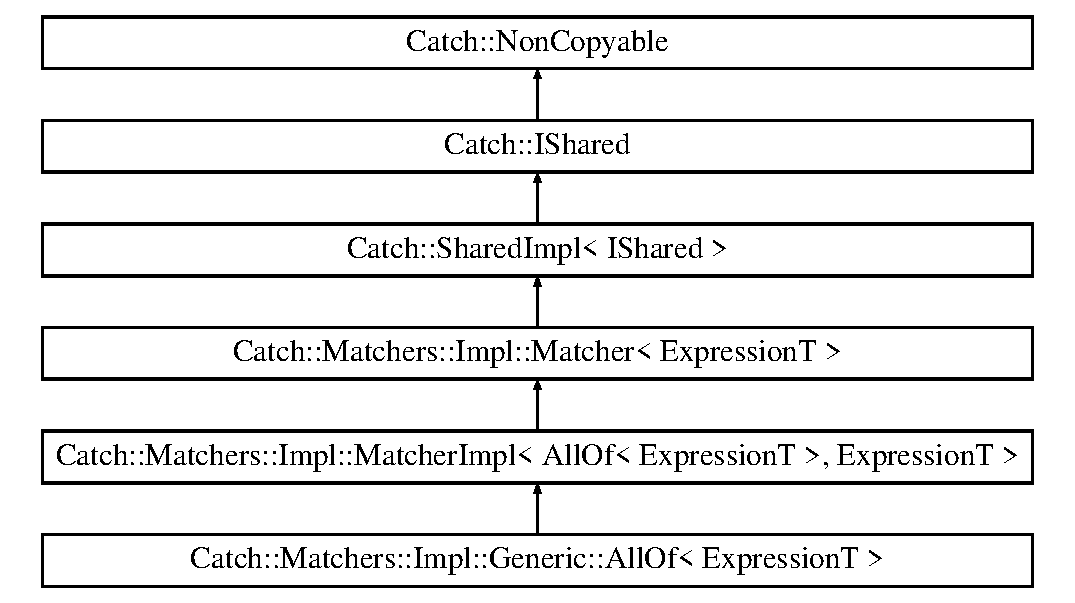
\includegraphics[height=6.000000cm]{class_catch_1_1_matchers_1_1_impl_1_1_generic_1_1_all_of}
\end{center}
\end{figure}
\subsection*{Public Member Functions}
\begin{DoxyCompactItemize}
\item 
\hypertarget{class_catch_1_1_matchers_1_1_impl_1_1_generic_1_1_all_of_a31f7c5e570e79bdf64064ee87c331a59}{{\bfseries All\-Of} (\hyperlink{class_catch_1_1_matchers_1_1_impl_1_1_generic_1_1_all_of}{All\-Of} const \&other)}\label{class_catch_1_1_matchers_1_1_impl_1_1_generic_1_1_all_of_a31f7c5e570e79bdf64064ee87c331a59}

\item 
\hypertarget{class_catch_1_1_matchers_1_1_impl_1_1_generic_1_1_all_of_a8c5cd1e494ab697076da418ee72ac297}{\hyperlink{class_catch_1_1_matchers_1_1_impl_1_1_generic_1_1_all_of}{All\-Of} \& {\bfseries add} (\hyperlink{struct_catch_1_1_matchers_1_1_impl_1_1_matcher}{Matcher}$<$ Expression\-T $>$ const \&matcher)}\label{class_catch_1_1_matchers_1_1_impl_1_1_generic_1_1_all_of_a8c5cd1e494ab697076da418ee72ac297}

\item 
\hypertarget{class_catch_1_1_matchers_1_1_impl_1_1_generic_1_1_all_of_a04534d0ac9e089f4500c3c19054f11ce}{virtual bool {\bfseries match} (Expression\-T const \&expr) const }\label{class_catch_1_1_matchers_1_1_impl_1_1_generic_1_1_all_of_a04534d0ac9e089f4500c3c19054f11ce}

\item 
\hypertarget{class_catch_1_1_matchers_1_1_impl_1_1_generic_1_1_all_of_a9febc1e67acbeff62a32bcbfdc0c8fab}{virtual std\-::string {\bfseries to\-String} () const }\label{class_catch_1_1_matchers_1_1_impl_1_1_generic_1_1_all_of_a9febc1e67acbeff62a32bcbfdc0c8fab}

\end{DoxyCompactItemize}
\subsection*{Additional Inherited Members}


The documentation for this class was generated from the following file\-:\begin{DoxyCompactItemize}
\item 
Catch.\-h\end{DoxyCompactItemize}

\hypertarget{class_catch_1_1_matchers_1_1_impl_1_1_generic_1_1_any_of}{\section{Catch\-:\-:Matchers\-:\-:Impl\-:\-:Generic\-:\-:Any\-Of$<$ Expression\-T $>$ Class Template Reference}
\label{class_catch_1_1_matchers_1_1_impl_1_1_generic_1_1_any_of}\index{Catch\-::\-Matchers\-::\-Impl\-::\-Generic\-::\-Any\-Of$<$ Expression\-T $>$@{Catch\-::\-Matchers\-::\-Impl\-::\-Generic\-::\-Any\-Of$<$ Expression\-T $>$}}
}
Inheritance diagram for Catch\-:\-:Matchers\-:\-:Impl\-:\-:Generic\-:\-:Any\-Of$<$ Expression\-T $>$\-:\begin{figure}[H]
\begin{center}
\leavevmode
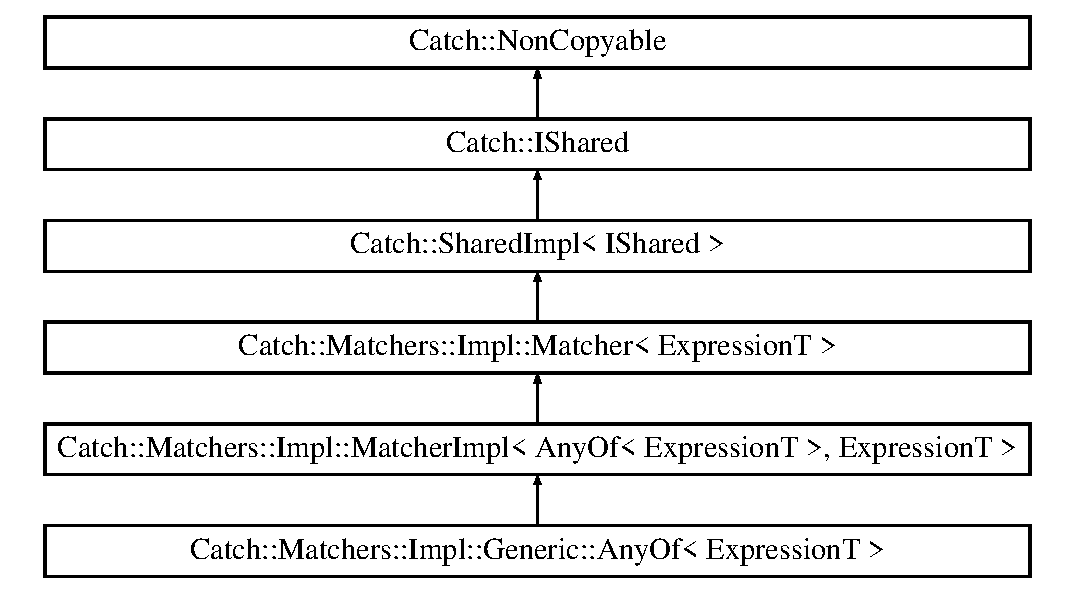
\includegraphics[height=6.000000cm]{class_catch_1_1_matchers_1_1_impl_1_1_generic_1_1_any_of}
\end{center}
\end{figure}
\subsection*{Public Member Functions}
\begin{DoxyCompactItemize}
\item 
\hypertarget{class_catch_1_1_matchers_1_1_impl_1_1_generic_1_1_any_of_a74fbc05b32d334fcbfd0fae0163a404e}{{\bfseries Any\-Of} (\hyperlink{class_catch_1_1_matchers_1_1_impl_1_1_generic_1_1_any_of}{Any\-Of} const \&other)}\label{class_catch_1_1_matchers_1_1_impl_1_1_generic_1_1_any_of_a74fbc05b32d334fcbfd0fae0163a404e}

\item 
\hypertarget{class_catch_1_1_matchers_1_1_impl_1_1_generic_1_1_any_of_a3bce94b627551e5f96c5f9c6060413f0}{\hyperlink{class_catch_1_1_matchers_1_1_impl_1_1_generic_1_1_any_of}{Any\-Of} \& {\bfseries add} (\hyperlink{struct_catch_1_1_matchers_1_1_impl_1_1_matcher}{Matcher}$<$ Expression\-T $>$ const \&matcher)}\label{class_catch_1_1_matchers_1_1_impl_1_1_generic_1_1_any_of_a3bce94b627551e5f96c5f9c6060413f0}

\item 
\hypertarget{class_catch_1_1_matchers_1_1_impl_1_1_generic_1_1_any_of_a2f97a08338e12deba541043a57d73db9}{virtual bool {\bfseries match} (Expression\-T const \&expr) const }\label{class_catch_1_1_matchers_1_1_impl_1_1_generic_1_1_any_of_a2f97a08338e12deba541043a57d73db9}

\item 
\hypertarget{class_catch_1_1_matchers_1_1_impl_1_1_generic_1_1_any_of_a7ecc6ec08b2018a643923a9d450aa328}{virtual std\-::string {\bfseries to\-String} () const }\label{class_catch_1_1_matchers_1_1_impl_1_1_generic_1_1_any_of_a7ecc6ec08b2018a643923a9d450aa328}

\end{DoxyCompactItemize}
\subsection*{Additional Inherited Members}


The documentation for this class was generated from the following file\-:\begin{DoxyCompactItemize}
\item 
Catch.\-h\end{DoxyCompactItemize}

\hypertarget{class_catch_1_1_detail_1_1_approx}{\section{Catch\-:\-:Detail\-:\-:Approx Class Reference}
\label{class_catch_1_1_detail_1_1_approx}\index{Catch\-::\-Detail\-::\-Approx@{Catch\-::\-Detail\-::\-Approx}}
}
\subsection*{Public Member Functions}
\begin{DoxyCompactItemize}
\item 
\hypertarget{class_catch_1_1_detail_1_1_approx_a1a8618ea8db08c66bd3d9fe8f74b957a}{{\bfseries Approx} (double value)}\label{class_catch_1_1_detail_1_1_approx_a1a8618ea8db08c66bd3d9fe8f74b957a}

\item 
\hypertarget{class_catch_1_1_detail_1_1_approx_a807330c63266fc914abdf6e461255a54}{{\bfseries Approx} (\hyperlink{class_catch_1_1_detail_1_1_approx}{Approx} const \&other)}\label{class_catch_1_1_detail_1_1_approx_a807330c63266fc914abdf6e461255a54}

\item 
\hypertarget{class_catch_1_1_detail_1_1_approx_a48c9cbc28a05dc9dc8c3973b9eae2268}{\hyperlink{class_catch_1_1_detail_1_1_approx}{Approx} {\bfseries operator()} (double value)}\label{class_catch_1_1_detail_1_1_approx_a48c9cbc28a05dc9dc8c3973b9eae2268}

\item 
\hypertarget{class_catch_1_1_detail_1_1_approx_a05c50c3ad0a971fab19345b5d94979a9}{\hyperlink{class_catch_1_1_detail_1_1_approx}{Approx} \& {\bfseries epsilon} (double new\-Epsilon)}\label{class_catch_1_1_detail_1_1_approx_a05c50c3ad0a971fab19345b5d94979a9}

\item 
\hypertarget{class_catch_1_1_detail_1_1_approx_acd80f0737bf38112beacd5ca95bef113}{\hyperlink{class_catch_1_1_detail_1_1_approx}{Approx} \& {\bfseries scale} (double new\-Scale)}\label{class_catch_1_1_detail_1_1_approx_acd80f0737bf38112beacd5ca95bef113}

\item 
\hypertarget{class_catch_1_1_detail_1_1_approx_adeb74b73506b3f6b2ba72aea15168fbe}{std\-::string {\bfseries to\-String} () const }\label{class_catch_1_1_detail_1_1_approx_adeb74b73506b3f6b2ba72aea15168fbe}

\end{DoxyCompactItemize}
\subsection*{Static Public Member Functions}
\begin{DoxyCompactItemize}
\item 
\hypertarget{class_catch_1_1_detail_1_1_approx_aaf86dc0ee92272ac2d9839197a07951d}{static \hyperlink{class_catch_1_1_detail_1_1_approx}{Approx} {\bfseries custom} ()}\label{class_catch_1_1_detail_1_1_approx_aaf86dc0ee92272ac2d9839197a07951d}

\end{DoxyCompactItemize}
\subsection*{Friends}
\begin{DoxyCompactItemize}
\item 
\hypertarget{class_catch_1_1_detail_1_1_approx_ac766f044f1c63f0c5997982baefd9049}{bool {\bfseries operator==} (double lhs, \hyperlink{class_catch_1_1_detail_1_1_approx}{Approx} const \&rhs)}\label{class_catch_1_1_detail_1_1_approx_ac766f044f1c63f0c5997982baefd9049}

\item 
\hypertarget{class_catch_1_1_detail_1_1_approx_a35999631e6cef569f9da9f3fa910db22}{bool {\bfseries operator==} (\hyperlink{class_catch_1_1_detail_1_1_approx}{Approx} const \&lhs, double rhs)}\label{class_catch_1_1_detail_1_1_approx_a35999631e6cef569f9da9f3fa910db22}

\item 
\hypertarget{class_catch_1_1_detail_1_1_approx_a83b3763569a7ecc143c335b630be0e47}{bool {\bfseries operator!=} (double lhs, \hyperlink{class_catch_1_1_detail_1_1_approx}{Approx} const \&rhs)}\label{class_catch_1_1_detail_1_1_approx_a83b3763569a7ecc143c335b630be0e47}

\item 
\hypertarget{class_catch_1_1_detail_1_1_approx_a7497ef839f8026cc0edd6269a80f3e09}{bool {\bfseries operator!=} (\hyperlink{class_catch_1_1_detail_1_1_approx}{Approx} const \&lhs, double rhs)}\label{class_catch_1_1_detail_1_1_approx_a7497ef839f8026cc0edd6269a80f3e09}

\end{DoxyCompactItemize}


The documentation for this class was generated from the following file\-:\begin{DoxyCompactItemize}
\item 
Catch.\-h\end{DoxyCompactItemize}

\hypertarget{struct_catch_1_1_assertion_info}{\section{Catch\-:\-:Assertion\-Info Struct Reference}
\label{struct_catch_1_1_assertion_info}\index{Catch\-::\-Assertion\-Info@{Catch\-::\-Assertion\-Info}}
}
\subsection*{Public Member Functions}
\begin{DoxyCompactItemize}
\item 
\hypertarget{struct_catch_1_1_assertion_info_aaf6cc3eebd40391e54d37ed42953c73f}{{\bfseries Assertion\-Info} (std\-::string const \&\-\_\-macro\-Name, \hyperlink{struct_catch_1_1_source_line_info}{Source\-Line\-Info} const \&\-\_\-line\-Info, std\-::string const \&\-\_\-captured\-Expression, Result\-Disposition\-::\-Flags \-\_\-result\-Disposition)}\label{struct_catch_1_1_assertion_info_aaf6cc3eebd40391e54d37ed42953c73f}

\end{DoxyCompactItemize}
\subsection*{Public Attributes}
\begin{DoxyCompactItemize}
\item 
\hypertarget{struct_catch_1_1_assertion_info_ac2e59e8c89e00eb3390768f50d540b18}{std\-::string {\bfseries macro\-Name}}\label{struct_catch_1_1_assertion_info_ac2e59e8c89e00eb3390768f50d540b18}

\item 
\hypertarget{struct_catch_1_1_assertion_info_a17bdbb404ba12658034f833be2f4c3e7}{\hyperlink{struct_catch_1_1_source_line_info}{Source\-Line\-Info} {\bfseries line\-Info}}\label{struct_catch_1_1_assertion_info_a17bdbb404ba12658034f833be2f4c3e7}

\item 
\hypertarget{struct_catch_1_1_assertion_info_af7c1d3cbfa346e9a303030fa0ef0cb54}{std\-::string {\bfseries captured\-Expression}}\label{struct_catch_1_1_assertion_info_af7c1d3cbfa346e9a303030fa0ef0cb54}

\item 
\hypertarget{struct_catch_1_1_assertion_info_a60353b3632ab2f827162f2b2d6911073}{Result\-Disposition\-::\-Flags {\bfseries result\-Disposition}}\label{struct_catch_1_1_assertion_info_a60353b3632ab2f827162f2b2d6911073}

\end{DoxyCompactItemize}


The documentation for this struct was generated from the following file\-:\begin{DoxyCompactItemize}
\item 
Catch.\-h\end{DoxyCompactItemize}

\hypertarget{class_catch_1_1_assertion_result}{\section{Catch\-:\-:Assertion\-Result Class Reference}
\label{class_catch_1_1_assertion_result}\index{Catch\-::\-Assertion\-Result@{Catch\-::\-Assertion\-Result}}
}
\subsection*{Public Member Functions}
\begin{DoxyCompactItemize}
\item 
\hypertarget{class_catch_1_1_assertion_result_ab58aeec27052ba400633ed0e36cea692}{{\bfseries Assertion\-Result} (\hyperlink{struct_catch_1_1_assertion_info}{Assertion\-Info} const \&info, \hyperlink{struct_catch_1_1_assertion_result_data}{Assertion\-Result\-Data} const \&data)}\label{class_catch_1_1_assertion_result_ab58aeec27052ba400633ed0e36cea692}

\item 
\hypertarget{class_catch_1_1_assertion_result_a70fb6aa62a38db3bdcafb4bb134afb21}{bool {\bfseries is\-Ok} () const }\label{class_catch_1_1_assertion_result_a70fb6aa62a38db3bdcafb4bb134afb21}

\item 
\hypertarget{class_catch_1_1_assertion_result_a5404062147930354afeb154de7cbaa7e}{bool {\bfseries succeeded} () const }\label{class_catch_1_1_assertion_result_a5404062147930354afeb154de7cbaa7e}

\item 
\hypertarget{class_catch_1_1_assertion_result_aa90bec8064879a62fcdc8e1079bcdba1}{Result\-Was\-::\-Of\-Type {\bfseries get\-Result\-Type} () const }\label{class_catch_1_1_assertion_result_aa90bec8064879a62fcdc8e1079bcdba1}

\item 
\hypertarget{class_catch_1_1_assertion_result_a45551f4f092c640ffce0cdd8a94f4b62}{bool {\bfseries has\-Expression} () const }\label{class_catch_1_1_assertion_result_a45551f4f092c640ffce0cdd8a94f4b62}

\item 
\hypertarget{class_catch_1_1_assertion_result_ab22a1c9baa182aeb2549fffeb8294d9e}{bool {\bfseries has\-Message} () const }\label{class_catch_1_1_assertion_result_ab22a1c9baa182aeb2549fffeb8294d9e}

\item 
\hypertarget{class_catch_1_1_assertion_result_a6105300b90d66b5c11b69813f83d074d}{std\-::string {\bfseries get\-Expression} () const }\label{class_catch_1_1_assertion_result_a6105300b90d66b5c11b69813f83d074d}

\item 
\hypertarget{class_catch_1_1_assertion_result_ac368a7490af7669decd58efea7d7dc54}{std\-::string {\bfseries get\-Expression\-In\-Macro} () const }\label{class_catch_1_1_assertion_result_ac368a7490af7669decd58efea7d7dc54}

\item 
\hypertarget{class_catch_1_1_assertion_result_a122c369bd49430a304e3eaebdf184f36}{bool {\bfseries has\-Expanded\-Expression} () const }\label{class_catch_1_1_assertion_result_a122c369bd49430a304e3eaebdf184f36}

\item 
\hypertarget{class_catch_1_1_assertion_result_a675d074588875eb62b0b6e36e05d65e6}{std\-::string {\bfseries get\-Expanded\-Expression} () const }\label{class_catch_1_1_assertion_result_a675d074588875eb62b0b6e36e05d65e6}

\item 
\hypertarget{class_catch_1_1_assertion_result_a9793bfc4d24678c8a013bda84a5aa905}{std\-::string {\bfseries get\-Message} () const }\label{class_catch_1_1_assertion_result_a9793bfc4d24678c8a013bda84a5aa905}

\item 
\hypertarget{class_catch_1_1_assertion_result_a68b73fe982a97fe6432af679af1a2dad}{\hyperlink{struct_catch_1_1_source_line_info}{Source\-Line\-Info} {\bfseries get\-Source\-Info} () const }\label{class_catch_1_1_assertion_result_a68b73fe982a97fe6432af679af1a2dad}

\item 
\hypertarget{class_catch_1_1_assertion_result_a2901d41b199258ff6a44571b147169dd}{std\-::string {\bfseries get\-Test\-Macro\-Name} () const }\label{class_catch_1_1_assertion_result_a2901d41b199258ff6a44571b147169dd}

\end{DoxyCompactItemize}
\subsection*{Protected Attributes}
\begin{DoxyCompactItemize}
\item 
\hypertarget{class_catch_1_1_assertion_result_a3e7236f73a51d6fc8bb9dfdefcee7772}{\hyperlink{struct_catch_1_1_assertion_info}{Assertion\-Info} {\bfseries m\-\_\-info}}\label{class_catch_1_1_assertion_result_a3e7236f73a51d6fc8bb9dfdefcee7772}

\item 
\hypertarget{class_catch_1_1_assertion_result_add3455b8bbedb0d643e18da67c66b4f7}{\hyperlink{struct_catch_1_1_assertion_result_data}{Assertion\-Result\-Data} {\bfseries m\-\_\-result\-Data}}\label{class_catch_1_1_assertion_result_add3455b8bbedb0d643e18da67c66b4f7}

\end{DoxyCompactItemize}


The documentation for this class was generated from the following file\-:\begin{DoxyCompactItemize}
\item 
Catch.\-h\end{DoxyCompactItemize}

\hypertarget{struct_catch_1_1_assertion_result_data}{\section{Catch\-:\-:Assertion\-Result\-Data Struct Reference}
\label{struct_catch_1_1_assertion_result_data}\index{Catch\-::\-Assertion\-Result\-Data@{Catch\-::\-Assertion\-Result\-Data}}
}
\subsection*{Public Attributes}
\begin{DoxyCompactItemize}
\item 
\hypertarget{struct_catch_1_1_assertion_result_data_a9e809d36fffbeb1c7d0cbe7382dd9595}{std\-::string {\bfseries reconstructed\-Expression}}\label{struct_catch_1_1_assertion_result_data_a9e809d36fffbeb1c7d0cbe7382dd9595}

\item 
\hypertarget{struct_catch_1_1_assertion_result_data_ac34215803c4c4a88f795879f61c1f7b4}{std\-::string {\bfseries message}}\label{struct_catch_1_1_assertion_result_data_ac34215803c4c4a88f795879f61c1f7b4}

\item 
\hypertarget{struct_catch_1_1_assertion_result_data_a7ceab4a7ff722aec5587e3748caf66b7}{Result\-Was\-::\-Of\-Type {\bfseries result\-Type}}\label{struct_catch_1_1_assertion_result_data_a7ceab4a7ff722aec5587e3748caf66b7}

\end{DoxyCompactItemize}


The documentation for this struct was generated from the following file\-:\begin{DoxyCompactItemize}
\item 
Catch.\-h\end{DoxyCompactItemize}

\hypertarget{struct_catch_1_1_assertion_stats}{\section{Catch\-:\-:Assertion\-Stats Struct Reference}
\label{struct_catch_1_1_assertion_stats}\index{Catch\-::\-Assertion\-Stats@{Catch\-::\-Assertion\-Stats}}
}
\subsection*{Public Member Functions}
\begin{DoxyCompactItemize}
\item 
\hypertarget{struct_catch_1_1_assertion_stats_a683d4c44ba214b9091cef80f4ee97967}{{\bfseries Assertion\-Stats} (\hyperlink{class_catch_1_1_assertion_result}{Assertion\-Result} const \&\-\_\-assertion\-Result, std\-::vector$<$ \hyperlink{struct_catch_1_1_message_info}{Message\-Info} $>$ const \&\-\_\-info\-Messages, \hyperlink{struct_catch_1_1_totals}{Totals} const \&\-\_\-totals)}\label{struct_catch_1_1_assertion_stats_a683d4c44ba214b9091cef80f4ee97967}

\end{DoxyCompactItemize}
\subsection*{Public Attributes}
\begin{DoxyCompactItemize}
\item 
\hypertarget{struct_catch_1_1_assertion_stats_a9f983a85332251f464efb4efba021b89}{\hyperlink{class_catch_1_1_assertion_result}{Assertion\-Result} {\bfseries assertion\-Result}}\label{struct_catch_1_1_assertion_stats_a9f983a85332251f464efb4efba021b89}

\item 
\hypertarget{struct_catch_1_1_assertion_stats_a12a032fa1f6e0fa8711946625758e6bb}{std\-::vector$<$ \hyperlink{struct_catch_1_1_message_info}{Message\-Info} $>$ {\bfseries info\-Messages}}\label{struct_catch_1_1_assertion_stats_a12a032fa1f6e0fa8711946625758e6bb}

\item 
\hypertarget{struct_catch_1_1_assertion_stats_a1cb537d44b8be3b19663f5fd1c25ce7a}{\hyperlink{struct_catch_1_1_totals}{Totals} {\bfseries totals}}\label{struct_catch_1_1_assertion_stats_a1cb537d44b8be3b19663f5fd1c25ce7a}

\end{DoxyCompactItemize}


The documentation for this struct was generated from the following file\-:\begin{DoxyCompactItemize}
\item 
Catch.\-h\end{DoxyCompactItemize}

\hypertarget{struct_catch_1_1_auto_reg}{\section{Catch\-:\-:Auto\-Reg Struct Reference}
\label{struct_catch_1_1_auto_reg}\index{Catch\-::\-Auto\-Reg@{Catch\-::\-Auto\-Reg}}
}
\subsection*{Public Member Functions}
\begin{DoxyCompactItemize}
\item 
\hypertarget{struct_catch_1_1_auto_reg_af224f4568d57b8652474df475a164a8c}{{\bfseries Auto\-Reg} (Test\-Function function, \hyperlink{struct_catch_1_1_source_line_info}{Source\-Line\-Info} const \&line\-Info, \hyperlink{struct_catch_1_1_name_and_desc}{Name\-And\-Desc} const \&name\-And\-Desc)}\label{struct_catch_1_1_auto_reg_af224f4568d57b8652474df475a164a8c}

\item 
\hypertarget{struct_catch_1_1_auto_reg_a1bf9207fe0a02b46dc0ab1cc03cbe738}{{\footnotesize template$<$typename C $>$ }\\{\bfseries Auto\-Reg} (void(C\-::$\ast$method)(), char const $\ast$class\-Name, \hyperlink{struct_catch_1_1_name_and_desc}{Name\-And\-Desc} const \&name\-And\-Desc, \hyperlink{struct_catch_1_1_source_line_info}{Source\-Line\-Info} const \&line\-Info)}\label{struct_catch_1_1_auto_reg_a1bf9207fe0a02b46dc0ab1cc03cbe738}

\item 
\hypertarget{struct_catch_1_1_auto_reg_a2dc6a03e838b31e29fcd6a740195b55b}{void {\bfseries register\-Test\-Case} (\hyperlink{struct_catch_1_1_i_test_case}{I\-Test\-Case} $\ast$test\-Case, char const $\ast$class\-Name, \hyperlink{struct_catch_1_1_name_and_desc}{Name\-And\-Desc} const \&name\-And\-Desc, \hyperlink{struct_catch_1_1_source_line_info}{Source\-Line\-Info} const \&line\-Info)}\label{struct_catch_1_1_auto_reg_a2dc6a03e838b31e29fcd6a740195b55b}

\end{DoxyCompactItemize}


The documentation for this struct was generated from the following file\-:\begin{DoxyCompactItemize}
\item 
Catch.\-h\end{DoxyCompactItemize}

\hypertarget{class_catch_1_1_between_generator}{\section{Catch\-:\-:Between\-Generator$<$ T $>$ Class Template Reference}
\label{class_catch_1_1_between_generator}\index{Catch\-::\-Between\-Generator$<$ T $>$@{Catch\-::\-Between\-Generator$<$ T $>$}}
}
Inheritance diagram for Catch\-:\-:Between\-Generator$<$ T $>$\-:\begin{figure}[H]
\begin{center}
\leavevmode
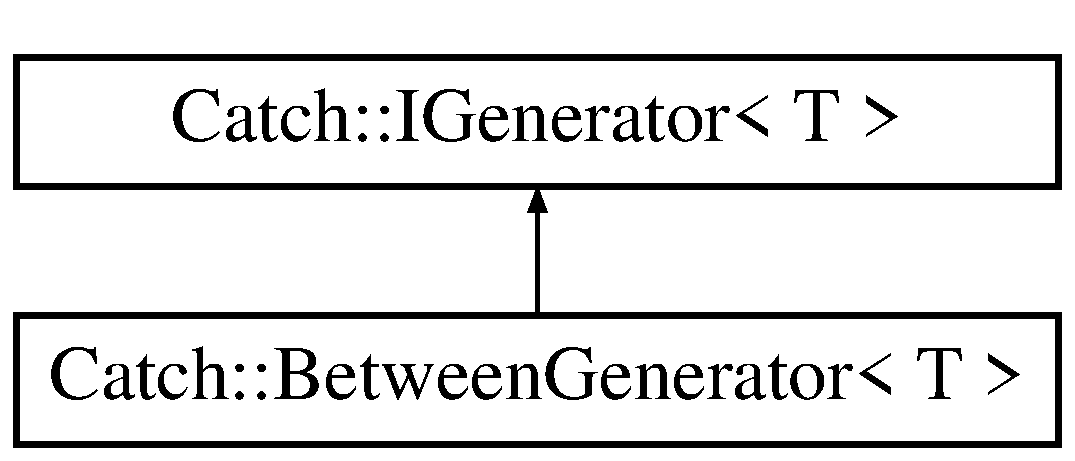
\includegraphics[height=2.000000cm]{class_catch_1_1_between_generator}
\end{center}
\end{figure}
\subsection*{Public Member Functions}
\begin{DoxyCompactItemize}
\item 
\hypertarget{class_catch_1_1_between_generator_a835a057d691ae37caef660624099b51c}{{\bfseries Between\-Generator} (T from, T to)}\label{class_catch_1_1_between_generator_a835a057d691ae37caef660624099b51c}

\item 
\hypertarget{class_catch_1_1_between_generator_af83575d62cc727ca995446cff4d6c26c}{virtual T {\bfseries get\-Value} (std\-::size\-\_\-t index) const }\label{class_catch_1_1_between_generator_af83575d62cc727ca995446cff4d6c26c}

\item 
\hypertarget{class_catch_1_1_between_generator_aa53a04a259e796ba2b5adabed79474b5}{virtual std\-::size\-\_\-t {\bfseries size} () const }\label{class_catch_1_1_between_generator_aa53a04a259e796ba2b5adabed79474b5}

\end{DoxyCompactItemize}


The documentation for this class was generated from the following file\-:\begin{DoxyCompactItemize}
\item 
Catch.\-h\end{DoxyCompactItemize}

\hypertarget{struct_catch_1_1_detail_1_1_borg_type}{\section{Catch\-:\-:Detail\-:\-:Borg\-Type Struct Reference}
\label{struct_catch_1_1_detail_1_1_borg_type}\index{Catch\-::\-Detail\-::\-Borg\-Type@{Catch\-::\-Detail\-::\-Borg\-Type}}
}
\subsection*{Public Member Functions}
\begin{DoxyCompactItemize}
\item 
\hypertarget{struct_catch_1_1_detail_1_1_borg_type_a780a9946ed0d654f0bfc043c8fc505d8}{{\footnotesize template$<$typename T $>$ }\\{\bfseries Borg\-Type} (T const \&)}\label{struct_catch_1_1_detail_1_1_borg_type_a780a9946ed0d654f0bfc043c8fc505d8}

\end{DoxyCompactItemize}


The documentation for this struct was generated from the following file\-:\begin{DoxyCompactItemize}
\item 
Catch.\-h\end{DoxyCompactItemize}

\hypertarget{class_c_f_g}{\section{C\-F\-G Class Reference}
\label{class_c_f_g}\index{C\-F\-G@{C\-F\-G}}
}


Class representing a context free grammar.  




{\ttfamily \#include $<$C\-F\-G.\-h$>$}

Inheritance diagram for C\-F\-G\-:\begin{figure}[H]
\begin{center}
\leavevmode
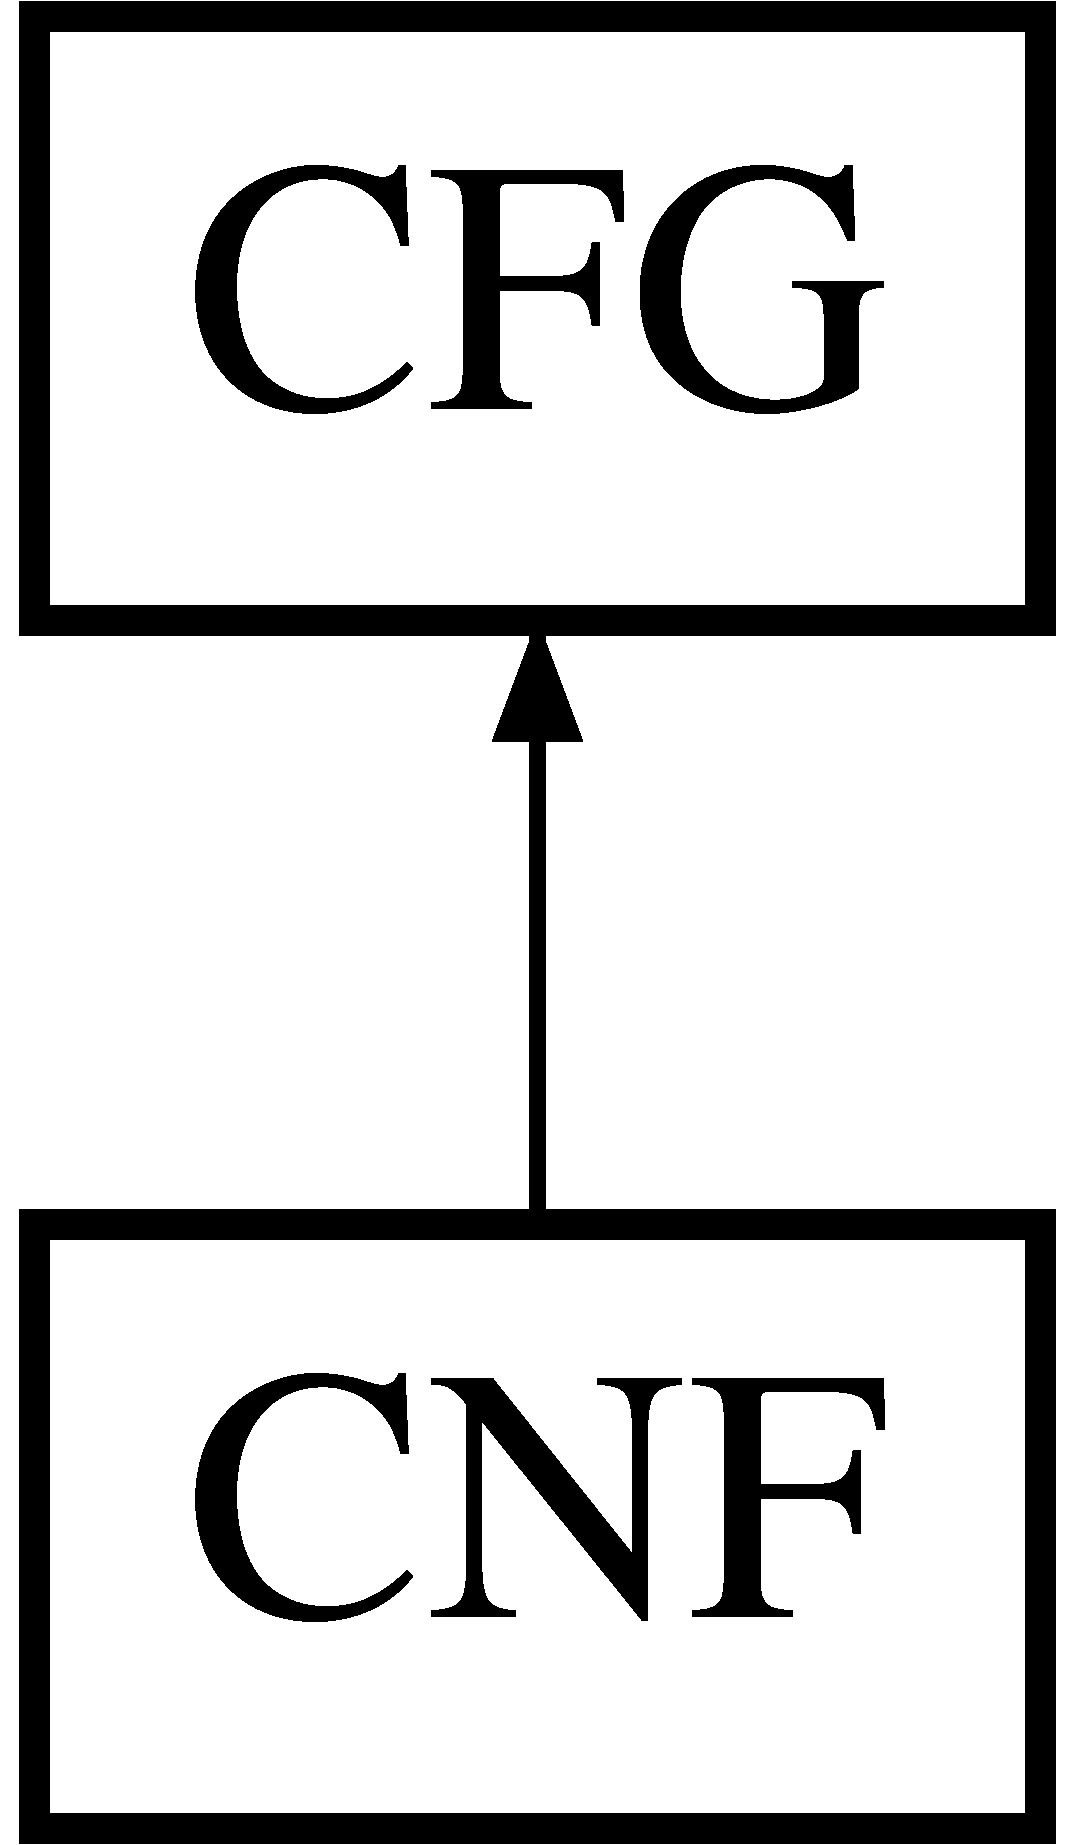
\includegraphics[height=2.000000cm]{class_c_f_g}
\end{center}
\end{figure}
\subsection*{Public Member Functions}
\begin{DoxyCompactItemize}
\item 
\hyperlink{class_c_f_g_a74681f6f1a182d0e754e5db0e9545f5b}{C\-F\-G} (const std\-::set$<$ char $>$ \&terminals, const std\-::set$<$ char $>$ \&variables, const std\-::multimap$<$ char, Symbol\-String $>$ \&productions, const char \&startsymbol)
\begin{DoxyCompactList}\small\item\em Constructor. \end{DoxyCompactList}\item 
\hypertarget{class_c_f_g_a7a9e0feb406099038faea4c67ef31786}{virtual \hyperlink{class_c_f_g_a7a9e0feb406099038faea4c67ef31786}{$\sim$\-C\-F\-G} ()}\label{class_c_f_g_a7a9e0feb406099038faea4c67ef31786}

\begin{DoxyCompactList}\small\item\em Destructor. \end{DoxyCompactList}\item 
std\-::set$<$ Symbol\-String $>$ \hyperlink{class_c_f_g_a391a7d2b5ef8145dff4c4b1d2c1dfe78}{bodies} (const char \&v) const 
\begin{DoxyCompactList}\small\item\em Get the set of bodies with the passed variable as head. For example if there are productions of the form A -\/$>$ \char`\"{}a\char`\"{} and A -\/$>$ \char`\"{}a\-A\char`\"{}, then this will returns \{\char`\"{}a\char`\"{}, \char`\"{}a\-A\char`\"{}\}. \end{DoxyCompactList}\item 
std\-::set$<$ char $>$ \hyperlink{class_c_f_g_a5df6f5e5f972ede1a2f1eb210a5e33d6}{nullable} () const 
\begin{DoxyCompactList}\small\item\em Get all the nullable variables. \end{DoxyCompactList}\item 
void \hyperlink{class_c_f_g_ac849b4a92eea2311a9626061b3e193b8}{eleminate\-Epsilon\-Productions} ()
\begin{DoxyCompactList}\small\item\em Eleminate epsilon productions. That is, eleminate productions of the form A -\/$>$ ε, but doing so that the \hyperlink{class_c_f_g}{C\-F\-G} still accepts the same language with epsilon (empty string excluded). \end{DoxyCompactList}\item 
std\-::set$<$ std\-::pair$<$ char, char $>$ $>$ \hyperlink{class_c_f_g_afe7d63958621b57a80d334827b9c6ceb}{units} () const 
\begin{DoxyCompactList}\small\item\em Get all the unit pairs of this \hyperlink{class_c_f_g}{C\-F\-G}. \end{DoxyCompactList}\item 
void \hyperlink{class_c_f_g_a61a4e75db20b0c39e0288c8f5146a8a6}{eleminate\-Unit\-Productions} ()
\begin{DoxyCompactList}\small\item\em Eleminate unit productions. That is, eleminate productions of the form A -\/$>$ B. But doing so that it does not affect the language of this \hyperlink{class_c_f_g}{C\-F\-G}. \end{DoxyCompactList}\item 
std\-::set$<$ char $>$ \hyperlink{class_c_f_g_ac6b8b908c8af9211ebecab911d5cd5ea}{generating} () const 
\begin{DoxyCompactList}\small\item\em Get all the generating symbols. \end{DoxyCompactList}\item 
std\-::set$<$ char $>$ \hyperlink{class_c_f_g_a41fd806703a8f2187abbefaa72a5cb5c}{reachable} () const 
\begin{DoxyCompactList}\small\item\em Get all the reachable symbols. \end{DoxyCompactList}\item 
void \hyperlink{class_c_f_g_a08b46d11fa9ce0670c1218d5231c20cb}{eleminate\-Useless\-Symbols} ()
\begin{DoxyCompactList}\small\item\em Eleminate useless symbols. But doing so that is does not affect the language of this \hyperlink{class_c_f_g}{C\-F\-G}. \end{DoxyCompactList}\item 
void \hyperlink{class_c_f_g_ab9999f6e214b05d9dfb0536b8b680e10}{clean\-Up} ()
\begin{DoxyCompactList}\small\item\em Clean up \hyperlink{class_c_f_g}{C\-F\-G}, that is, eleminate epsilon productions, useless symbols and unit productions I\-N S\-A\-F\-E O\-R\-D\-E\-R. This comes in handy for converting to \hyperlink{class_c_n_f}{C\-N\-F} (Chomsky Normal Form). Also\-: removes all variables which don't have any production rules at all. \end{DoxyCompactList}\item 
\hypertarget{class_c_f_g_a49b4255577be81ace0b957bd05ffcc4e}{std\-::set$<$ char $>$ {\bfseries get\-Terminals} ()}\label{class_c_f_g_a49b4255577be81ace0b957bd05ffcc4e}

\item 
\hypertarget{class_c_f_g_a93e29d2502f3189e7f7a9808d3871537}{std\-::set$<$ char $>$ {\bfseries get\-Variables} ()}\label{class_c_f_g_a93e29d2502f3189e7f7a9808d3871537}

\item 
\hypertarget{class_c_f_g_aa3831e04435bec5137fbf8ec99342d53}{std\-::multimap$<$ char, Symbol\-String $>$ {\bfseries get\-Productions} ()}\label{class_c_f_g_aa3831e04435bec5137fbf8ec99342d53}

\item 
\hypertarget{class_c_f_g_a7f285339723a8cbe79dcf3fc4eb1c551}{char {\bfseries get\-Startsymbol} ()}\label{class_c_f_g_a7f285339723a8cbe79dcf3fc4eb1c551}

\end{DoxyCompactItemize}
\subsection*{Protected Attributes}
\begin{DoxyCompactItemize}
\item 
\hypertarget{class_c_f_g_ac016cd234680353c2335233b9e46cb47}{std\-::set$<$ char $>$ \hyperlink{class_c_f_g_ac016cd234680353c2335233b9e46cb47}{f\-Terminals}}\label{class_c_f_g_ac016cd234680353c2335233b9e46cb47}

\begin{DoxyCompactList}\small\item\em The set of terminal symbols. \end{DoxyCompactList}\item 
\hypertarget{class_c_f_g_a2782ff517d0b17f6ae3853dae83ed144}{std\-::set$<$ char $>$ \hyperlink{class_c_f_g_a2782ff517d0b17f6ae3853dae83ed144}{f\-Variables}}\label{class_c_f_g_a2782ff517d0b17f6ae3853dae83ed144}

\begin{DoxyCompactList}\small\item\em The set of variables. \end{DoxyCompactList}\item 
\hypertarget{class_c_f_g_acead5f2b9238ec9bbc56d9e1de16f44f}{std\-::multimap$<$ char, Symbol\-String $>$ \hyperlink{class_c_f_g_acead5f2b9238ec9bbc56d9e1de16f44f}{f\-Productions}}\label{class_c_f_g_acead5f2b9238ec9bbc56d9e1de16f44f}

\begin{DoxyCompactList}\small\item\em The set of production rules. \end{DoxyCompactList}\item 
\hypertarget{class_c_f_g_acb92bc7a21984ef4a6d6a86b2e2e1b53}{char {\bfseries f\-Start\-Symbol}}\label{class_c_f_g_acb92bc7a21984ef4a6d6a86b2e2e1b53}

\end{DoxyCompactItemize}


\subsection{Detailed Description}
Class representing a context free grammar. 

\subsection{Constructor \& Destructor Documentation}
\hypertarget{class_c_f_g_a74681f6f1a182d0e754e5db0e9545f5b}{\index{C\-F\-G@{C\-F\-G}!C\-F\-G@{C\-F\-G}}
\index{C\-F\-G@{C\-F\-G}!CFG@{C\-F\-G}}
\subsubsection[{C\-F\-G}]{\setlength{\rightskip}{0pt plus 5cm}C\-F\-G\-::\-C\-F\-G (
\begin{DoxyParamCaption}
\item[{const std\-::set$<$ char $>$ \&}]{terminals, }
\item[{const std\-::set$<$ char $>$ \&}]{variables, }
\item[{const std\-::multimap$<$ char, Symbol\-String $>$ \&}]{productions, }
\item[{const char \&}]{startsymbol}
\end{DoxyParamCaption}
)}}\label{class_c_f_g_a74681f6f1a182d0e754e5db0e9545f5b}


Constructor. 


\begin{DoxyParams}{Parameters}
{\em terminals} & A set containing the terminals of the \hyperlink{class_c_f_g}{C\-F\-G}. \\
\hline
{\em variables} & A set containing the variables of the \hyperlink{class_c_f_g}{C\-F\-G}. \\
\hline
{\em productions} & A multimap that maps any symbol from the set of variables to a (possibly empty) Symbol\-String (which contains symbols from either the set of terminals or either the set of variables. \\
\hline
{\em startsymbol} & The startsymbol for the \hyperlink{class_c_f_g}{C\-F\-G}.\\
\hline
\end{DoxyParams}
\begin{DoxyPrecond}{Precondition}

\begin{DoxyItemize}
\item The set of variables and the set of terminals are disjoints.
\item The production rule is valid\-: the head consist of exactly one symbol that is in the set of the variables and the body must be empty or consisting of symbols that is either in the set of variables or in the set of terminals.
\item The starting symbol must be a member of the set of variables.
\end{DoxyItemize}
\end{DoxyPrecond}

\begin{DoxyExceptions}{Exceptions}
{\em std\-::invalid\-\_\-argument} & One of the preconditions were not met. \\
\hline
\end{DoxyExceptions}


\subsection{Member Function Documentation}
\hypertarget{class_c_f_g_a391a7d2b5ef8145dff4c4b1d2c1dfe78}{\index{C\-F\-G@{C\-F\-G}!bodies@{bodies}}
\index{bodies@{bodies}!CFG@{C\-F\-G}}
\subsubsection[{bodies}]{\setlength{\rightskip}{0pt plus 5cm}std\-::set$<$ Symbol\-String $>$ C\-F\-G\-::bodies (
\begin{DoxyParamCaption}
\item[{const char \&}]{v}
\end{DoxyParamCaption}
) const}}\label{class_c_f_g_a391a7d2b5ef8145dff4c4b1d2c1dfe78}


Get the set of bodies with the passed variable as head. For example if there are productions of the form A -\/$>$ \char`\"{}a\char`\"{} and A -\/$>$ \char`\"{}a\-A\char`\"{}, then this will returns \{\char`\"{}a\char`\"{}, \char`\"{}a\-A\char`\"{}\}. 


\begin{DoxyParams}{Parameters}
{\em v} & The variable representing the head of the production rules.\\
\hline
\end{DoxyParams}
\begin{DoxyReturn}{Returns}
The set of Symbol\-String representing the body of the production rules whose head is the passed variable.
\end{DoxyReturn}
\begin{DoxyPrecond}{Precondition}

\begin{DoxyItemize}
\item The passed variable must be in the set of the variables.
\end{DoxyItemize}
\end{DoxyPrecond}

\begin{DoxyExceptions}{Exceptions}
{\em std\-::invalid\-\_\-argument} & The precondition were not satisfied. \\
\hline
\end{DoxyExceptions}
\hypertarget{class_c_f_g_ab9999f6e214b05d9dfb0536b8b680e10}{\index{C\-F\-G@{C\-F\-G}!clean\-Up@{clean\-Up}}
\index{clean\-Up@{clean\-Up}!CFG@{C\-F\-G}}
\subsubsection[{clean\-Up}]{\setlength{\rightskip}{0pt plus 5cm}void C\-F\-G\-::clean\-Up (
\begin{DoxyParamCaption}
{}
\end{DoxyParamCaption}
)}}\label{class_c_f_g_ab9999f6e214b05d9dfb0536b8b680e10}


Clean up \hyperlink{class_c_f_g}{C\-F\-G}, that is, eleminate epsilon productions, useless symbols and unit productions I\-N S\-A\-F\-E O\-R\-D\-E\-R. This comes in handy for converting to \hyperlink{class_c_n_f}{C\-N\-F} (Chomsky Normal Form). Also\-: removes all variables which don't have any production rules at all. 

\begin{DoxyPostcond}{Postcondition}
The production rules doesn't contain any nullable symbols. 

The production rules doesn't contain any useless symbols. 

The \hyperlink{class_c_f_g}{C\-F\-G} has only unit pairs of the form (A, A) for each A is a variable. 
\end{DoxyPostcond}
\hypertarget{class_c_f_g_ac849b4a92eea2311a9626061b3e193b8}{\index{C\-F\-G@{C\-F\-G}!eleminate\-Epsilon\-Productions@{eleminate\-Epsilon\-Productions}}
\index{eleminate\-Epsilon\-Productions@{eleminate\-Epsilon\-Productions}!CFG@{C\-F\-G}}
\subsubsection[{eleminate\-Epsilon\-Productions}]{\setlength{\rightskip}{0pt plus 5cm}void C\-F\-G\-::eleminate\-Epsilon\-Productions (
\begin{DoxyParamCaption}
{}
\end{DoxyParamCaption}
)}}\label{class_c_f_g_ac849b4a92eea2311a9626061b3e193b8}


Eleminate epsilon productions. That is, eleminate productions of the form A -\/$>$ ε, but doing so that the \hyperlink{class_c_f_g}{C\-F\-G} still accepts the same language with epsilon (empty string excluded). 

\begin{DoxyPostcond}{Postcondition}
The production rules doesn't contain any nullable symbols. 
\end{DoxyPostcond}
\hypertarget{class_c_f_g_a61a4e75db20b0c39e0288c8f5146a8a6}{\index{C\-F\-G@{C\-F\-G}!eleminate\-Unit\-Productions@{eleminate\-Unit\-Productions}}
\index{eleminate\-Unit\-Productions@{eleminate\-Unit\-Productions}!CFG@{C\-F\-G}}
\subsubsection[{eleminate\-Unit\-Productions}]{\setlength{\rightskip}{0pt plus 5cm}void C\-F\-G\-::eleminate\-Unit\-Productions (
\begin{DoxyParamCaption}
{}
\end{DoxyParamCaption}
)}}\label{class_c_f_g_a61a4e75db20b0c39e0288c8f5146a8a6}


Eleminate unit productions. That is, eleminate productions of the form A -\/$>$ B. But doing so that it does not affect the language of this \hyperlink{class_c_f_g}{C\-F\-G}. 

\begin{DoxyNote}{Note}
The algorithm only works if there is no cycle of unit productions. That is, unit pairs of the form A -\/$>$ B, B -\/$>$ C and C -\/$>$ A. If that's the case, an exception will be thrown.
\end{DoxyNote}

\begin{DoxyExceptions}{Exceptions}
{\em std\-::logic\-\_\-error} & This \hyperlink{class_c_f_g}{C\-F\-G} has a cycle of unit pairs. T\-O\-D\-O\\
\hline
\end{DoxyExceptions}
\begin{DoxyPostcond}{Postcondition}
The \hyperlink{class_c_f_g}{C\-F\-G} has only unit pairs of the form (A, A) for each A is a variable. 
\end{DoxyPostcond}
\hypertarget{class_c_f_g_a08b46d11fa9ce0670c1218d5231c20cb}{\index{C\-F\-G@{C\-F\-G}!eleminate\-Useless\-Symbols@{eleminate\-Useless\-Symbols}}
\index{eleminate\-Useless\-Symbols@{eleminate\-Useless\-Symbols}!CFG@{C\-F\-G}}
\subsubsection[{eleminate\-Useless\-Symbols}]{\setlength{\rightskip}{0pt plus 5cm}void C\-F\-G\-::eleminate\-Useless\-Symbols (
\begin{DoxyParamCaption}
{}
\end{DoxyParamCaption}
)}}\label{class_c_f_g_a08b46d11fa9ce0670c1218d5231c20cb}


Eleminate useless symbols. But doing so that is does not affect the language of this \hyperlink{class_c_f_g}{C\-F\-G}. 

\begin{DoxyPostcond}{Postcondition}
The production rules doesn't contain any useless symbols. 

The \hyperlink{class_c_f_g}{C\-F\-G} still accepts the same language. 
\end{DoxyPostcond}
\hypertarget{class_c_f_g_ac6b8b908c8af9211ebecab911d5cd5ea}{\index{C\-F\-G@{C\-F\-G}!generating@{generating}}
\index{generating@{generating}!CFG@{C\-F\-G}}
\subsubsection[{generating}]{\setlength{\rightskip}{0pt plus 5cm}std\-::set$<$ char $>$ C\-F\-G\-::generating (
\begin{DoxyParamCaption}
{}
\end{DoxyParamCaption}
) const}}\label{class_c_f_g_ac6b8b908c8af9211ebecab911d5cd5ea}


Get all the generating symbols. 

\begin{DoxyReturn}{Returns}
The set of generating symbols. 
\end{DoxyReturn}
\hypertarget{class_c_f_g_a5df6f5e5f972ede1a2f1eb210a5e33d6}{\index{C\-F\-G@{C\-F\-G}!nullable@{nullable}}
\index{nullable@{nullable}!CFG@{C\-F\-G}}
\subsubsection[{nullable}]{\setlength{\rightskip}{0pt plus 5cm}std\-::set$<$ char $>$ C\-F\-G\-::nullable (
\begin{DoxyParamCaption}
{}
\end{DoxyParamCaption}
) const}}\label{class_c_f_g_a5df6f5e5f972ede1a2f1eb210a5e33d6}


Get all the nullable variables. 

\begin{DoxyReturn}{Returns}
The set of all nullable variables. 
\end{DoxyReturn}
\hypertarget{class_c_f_g_a41fd806703a8f2187abbefaa72a5cb5c}{\index{C\-F\-G@{C\-F\-G}!reachable@{reachable}}
\index{reachable@{reachable}!CFG@{C\-F\-G}}
\subsubsection[{reachable}]{\setlength{\rightskip}{0pt plus 5cm}std\-::set$<$ char $>$ C\-F\-G\-::reachable (
\begin{DoxyParamCaption}
{}
\end{DoxyParamCaption}
) const}}\label{class_c_f_g_a41fd806703a8f2187abbefaa72a5cb5c}


Get all the reachable symbols. 

\begin{DoxyReturn}{Returns}
The set of all reachable symbols. 
\end{DoxyReturn}
\hypertarget{class_c_f_g_afe7d63958621b57a80d334827b9c6ceb}{\index{C\-F\-G@{C\-F\-G}!units@{units}}
\index{units@{units}!CFG@{C\-F\-G}}
\subsubsection[{units}]{\setlength{\rightskip}{0pt plus 5cm}std\-::set$<$ std\-::pair$<$ char, char $>$ $>$ C\-F\-G\-::units (
\begin{DoxyParamCaption}
{}
\end{DoxyParamCaption}
) const}}\label{class_c_f_g_afe7d63958621b57a80d334827b9c6ceb}


Get all the unit pairs of this \hyperlink{class_c_f_g}{C\-F\-G}. 

\begin{DoxyReturn}{Returns}
The set of all unit pairs. 
\end{DoxyReturn}


The documentation for this class was generated from the following files\-:\begin{DoxyCompactItemize}
\item 
C\-F\-G.\-h\item 
C\-F\-G.\-cpp\end{DoxyCompactItemize}

\hypertarget{class_c_n_f}{\section{C\-N\-F Class Reference}
\label{class_c_n_f}\index{C\-N\-F@{C\-N\-F}}
}


The class \hyperlink{class_c_n_f}{C\-N\-F} (Chomsky Normal Form), this is actually a \hyperlink{class_c_f_g}{C\-F\-G} (Context Free Grammar) but with production rules of the form\-:  




{\ttfamily \#include $<$C\-N\-F.\-h$>$}

Inheritance diagram for C\-N\-F\-:\begin{figure}[H]
\begin{center}
\leavevmode
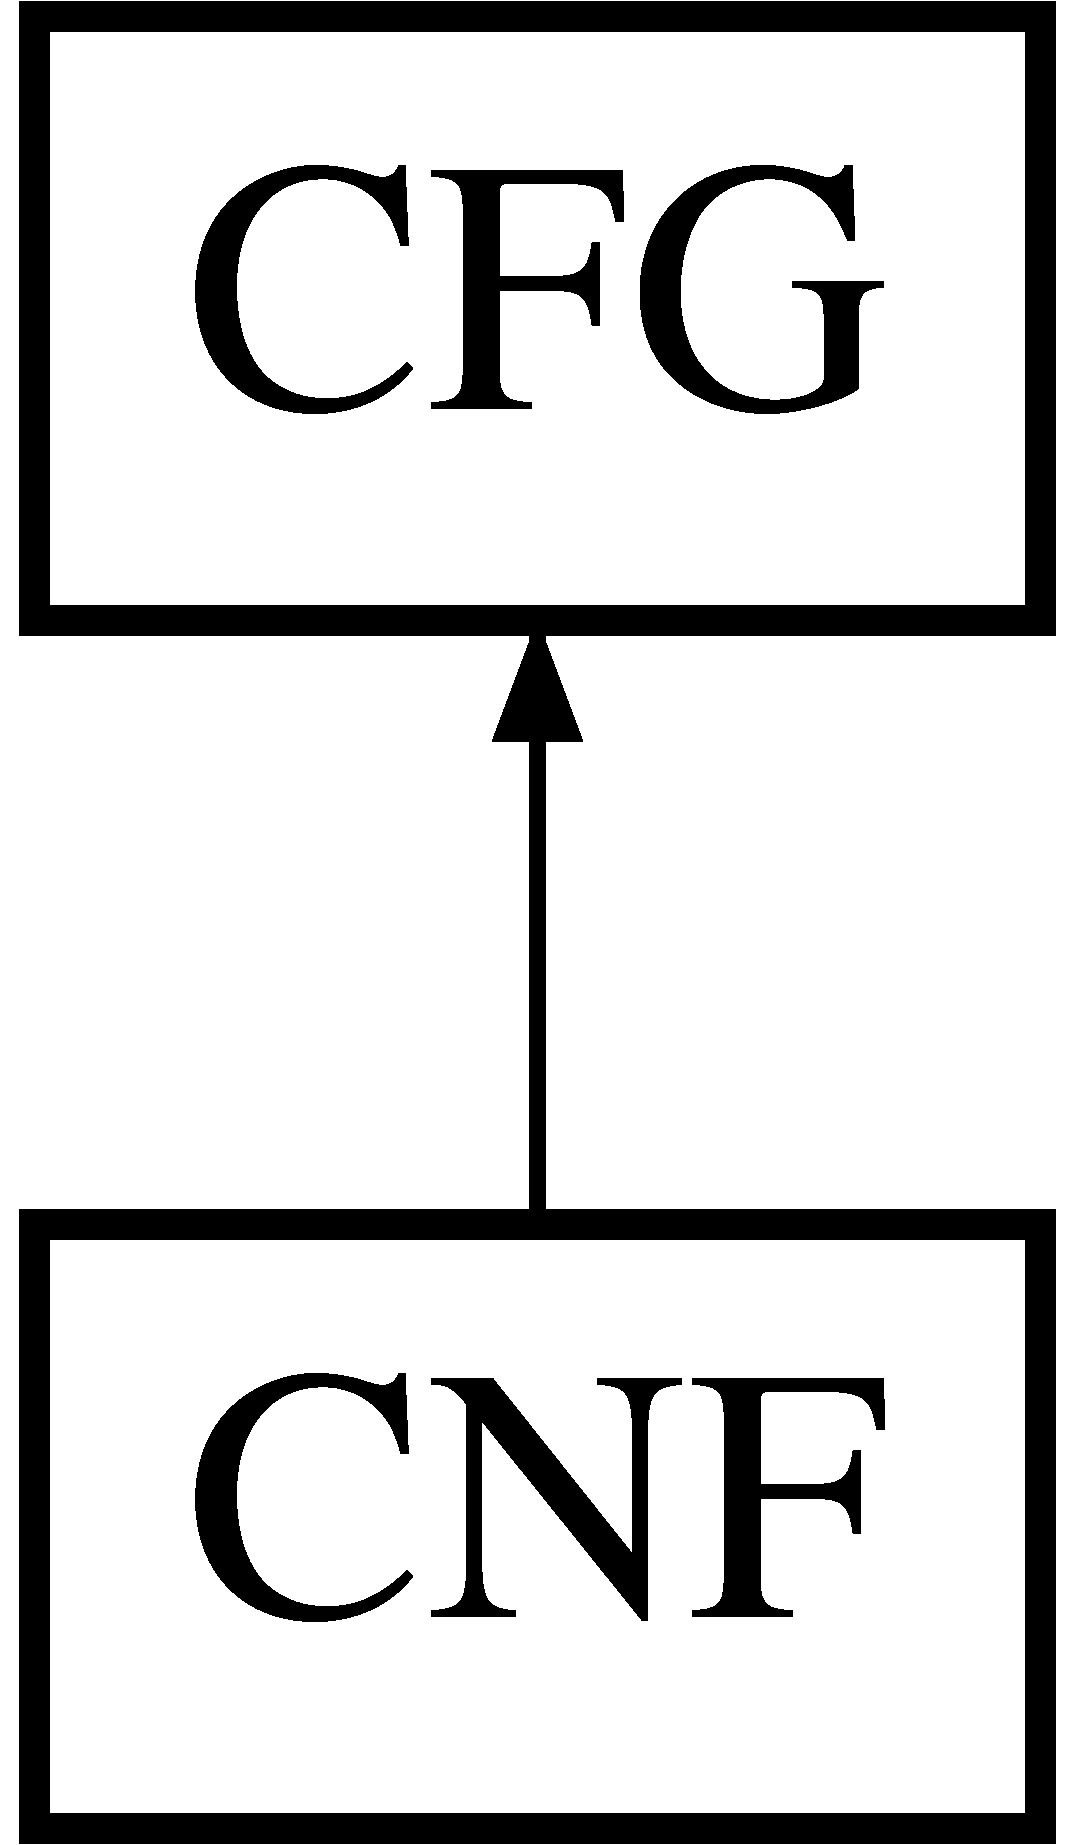
\includegraphics[height=2.000000cm]{class_c_n_f}
\end{center}
\end{figure}
\subsection*{Public Member Functions}
\begin{DoxyCompactItemize}
\item 
\hyperlink{class_c_n_f_a284b4ec60a90f49dabba546ea637a345}{C\-N\-F} (const std\-::set$<$ char $>$ \&terminals, const std\-::set$<$ char $>$ \&variables, const std\-::multimap$<$ char, Symbol\-String $>$ \&productions, const char \&start)
\begin{DoxyCompactList}\small\item\em Constructor, initialize all datamembers. This will construct production rules based upon the rules of the \hyperlink{class_c_f_g}{C\-F\-G} cleaned up variant and satisfying the conditions imposed by the \hyperlink{class_c_n_f}{C\-N\-F}. \end{DoxyCompactList}\item 
bool \hyperlink{class_c_n_f_ae6dd043b79759b038cd627267bf7295c}{C\-Y\-K} (const std\-::string \&terminalstring) const 
\begin{DoxyCompactList}\small\item\em Check whether the terminalstring is in the language of this \hyperlink{class_c_n_f}{C\-N\-F} by using the C\-Y\-K algorithm. \end{DoxyCompactList}\end{DoxyCompactItemize}
\subsection*{Additional Inherited Members}


\subsection{Detailed Description}
The class \hyperlink{class_c_n_f}{C\-N\-F} (Chomsky Normal Form), this is actually a \hyperlink{class_c_f_g}{C\-F\-G} (Context Free Grammar) but with production rules of the form\-: 


\begin{DoxyItemize}
\item A --$>$ B\-C (with A, B and C variables) or
\item A --$>$ a (with A a variable and a a terminal) 
\end{DoxyItemize}

\subsection{Constructor \& Destructor Documentation}
\hypertarget{class_c_n_f_a284b4ec60a90f49dabba546ea637a345}{\index{C\-N\-F@{C\-N\-F}!C\-N\-F@{C\-N\-F}}
\index{C\-N\-F@{C\-N\-F}!CNF@{C\-N\-F}}
\subsubsection[{C\-N\-F}]{\setlength{\rightskip}{0pt plus 5cm}C\-N\-F\-::\-C\-N\-F (
\begin{DoxyParamCaption}
\item[{const std\-::set$<$ char $>$ \&}]{terminals, }
\item[{const std\-::set$<$ char $>$ \&}]{variables, }
\item[{const std\-::multimap$<$ char, Symbol\-String $>$ \&}]{productions, }
\item[{const char \&}]{start}
\end{DoxyParamCaption}
)}}\label{class_c_n_f_a284b4ec60a90f49dabba546ea637a345}


Constructor, initialize all datamembers. This will construct production rules based upon the rules of the \hyperlink{class_c_f_g}{C\-F\-G} cleaned up variant and satisfying the conditions imposed by the \hyperlink{class_c_n_f}{C\-N\-F}. 

\begin{DoxyNote}{Note}
You can still use the \hyperlink{class_c_f_g}{C\-F\-G} methods as if it was only cleaned up (thus you can use the same variables for getting the bodies and such).
\end{DoxyNote}

\begin{DoxyParams}{Parameters}
{\em terminals} & The set of terminal symbols. \\
\hline
{\em variables} & The set of non-\/terminal symbols. \\
\hline
{\em productions} & The set of production rules (which is actually a std\-::map where each non-\/terminal symbol maps to a string consisting of terminals and variables. \\
\hline
{\em start} & The start symbol.\\
\hline
\end{DoxyParams}
\begin{DoxyPostcond}{Postcondition}

\begin{DoxyItemize}
\item The \hyperlink{class_c_f_g}{C\-F\-G} methods will produce the same result as if it was already cleaned up without unwanted side-\/effects. 
\end{DoxyItemize}
\end{DoxyPostcond}


\subsection{Member Function Documentation}
\hypertarget{class_c_n_f_ae6dd043b79759b038cd627267bf7295c}{\index{C\-N\-F@{C\-N\-F}!C\-Y\-K@{C\-Y\-K}}
\index{C\-Y\-K@{C\-Y\-K}!CNF@{C\-N\-F}}
\subsubsection[{C\-Y\-K}]{\setlength{\rightskip}{0pt plus 5cm}bool C\-N\-F\-::\-C\-Y\-K (
\begin{DoxyParamCaption}
\item[{const std\-::string \&}]{terminalstring}
\end{DoxyParamCaption}
) const}}\label{class_c_n_f_ae6dd043b79759b038cd627267bf7295c}


Check whether the terminalstring is in the language of this \hyperlink{class_c_n_f}{C\-N\-F} by using the C\-Y\-K algorithm. 


\begin{DoxyParams}{Parameters}
{\em terminalstring} & The string to be checked whether this is in the language of the \hyperlink{class_c_f_g}{C\-F\-G}.\\
\hline
\end{DoxyParams}
\begin{DoxyReturn}{Returns}
True if the terminalstring is in the language of this \hyperlink{class_c_f_g}{C\-F\-G}, false if not.
\end{DoxyReturn}
\begin{DoxyPrecond}{Precondition}

\begin{DoxyItemize}
\item The string passed consists only of terminal symbols in the set of terminals of this \hyperlink{class_c_f_g}{C\-F\-G}.
\end{DoxyItemize}
\end{DoxyPrecond}

\begin{DoxyExceptions}{Exceptions}
{\em std\-::invalid\-\_\-argument} & if the string passed is not a valid terminal string (that is, not consisting of terminal symbols). \\
\hline
\end{DoxyExceptions}


The documentation for this class was generated from the following files\-:\begin{DoxyCompactItemize}
\item 
C\-N\-F.\-h\item 
C\-N\-F.\-cpp\end{DoxyCompactItemize}

\hypertarget{class_catch_1_1_composite_generator}{\section{Catch\-:\-:Composite\-Generator$<$ T $>$ Class Template Reference}
\label{class_catch_1_1_composite_generator}\index{Catch\-::\-Composite\-Generator$<$ T $>$@{Catch\-::\-Composite\-Generator$<$ T $>$}}
}
\subsection*{Public Member Functions}
\begin{DoxyCompactItemize}
\item 
\hypertarget{class_catch_1_1_composite_generator_a21a7070a00e4a6fe021294c356692692}{{\bfseries Composite\-Generator} (\hyperlink{class_catch_1_1_composite_generator}{Composite\-Generator} \&other)}\label{class_catch_1_1_composite_generator_a21a7070a00e4a6fe021294c356692692}

\item 
\hypertarget{class_catch_1_1_composite_generator_ac3c57cf4ca5472f440bf71e2936bcd4a}{\hyperlink{class_catch_1_1_composite_generator}{Composite\-Generator} \& {\bfseries set\-File\-Info} (const char $\ast$file\-Info)}\label{class_catch_1_1_composite_generator_ac3c57cf4ca5472f440bf71e2936bcd4a}

\item 
\hypertarget{class_catch_1_1_composite_generator_aa3f627d84fb256df0404d19d7fd4b784}{{\bfseries operator T} () const }\label{class_catch_1_1_composite_generator_aa3f627d84fb256df0404d19d7fd4b784}

\item 
\hypertarget{class_catch_1_1_composite_generator_af3774d42ad2d3453d089ca599efe0517}{void {\bfseries add} (const \hyperlink{struct_catch_1_1_i_generator}{I\-Generator}$<$ T $>$ $\ast$generator)}\label{class_catch_1_1_composite_generator_af3774d42ad2d3453d089ca599efe0517}

\item 
\hypertarget{class_catch_1_1_composite_generator_a2e03f42df85cdd238aabd77a80b075d5}{\hyperlink{class_catch_1_1_composite_generator}{Composite\-Generator} \& {\bfseries then} (\hyperlink{class_catch_1_1_composite_generator}{Composite\-Generator} \&other)}\label{class_catch_1_1_composite_generator_a2e03f42df85cdd238aabd77a80b075d5}

\item 
\hypertarget{class_catch_1_1_composite_generator_aefdc11bcfccdf07d2db5f0da3ed8758c}{\hyperlink{class_catch_1_1_composite_generator}{Composite\-Generator} \& {\bfseries then} (T value)}\label{class_catch_1_1_composite_generator_aefdc11bcfccdf07d2db5f0da3ed8758c}

\end{DoxyCompactItemize}


The documentation for this class was generated from the following file\-:\begin{DoxyCompactItemize}
\item 
Catch.\-h\end{DoxyCompactItemize}

\hypertarget{class_catch_1_1_config}{\section{Catch\-:\-:Config Class Reference}
\label{class_catch_1_1_config}\index{Catch\-::\-Config@{Catch\-::\-Config}}
}
Inheritance diagram for Catch\-:\-:Config\-:\begin{figure}[H]
\begin{center}
\leavevmode
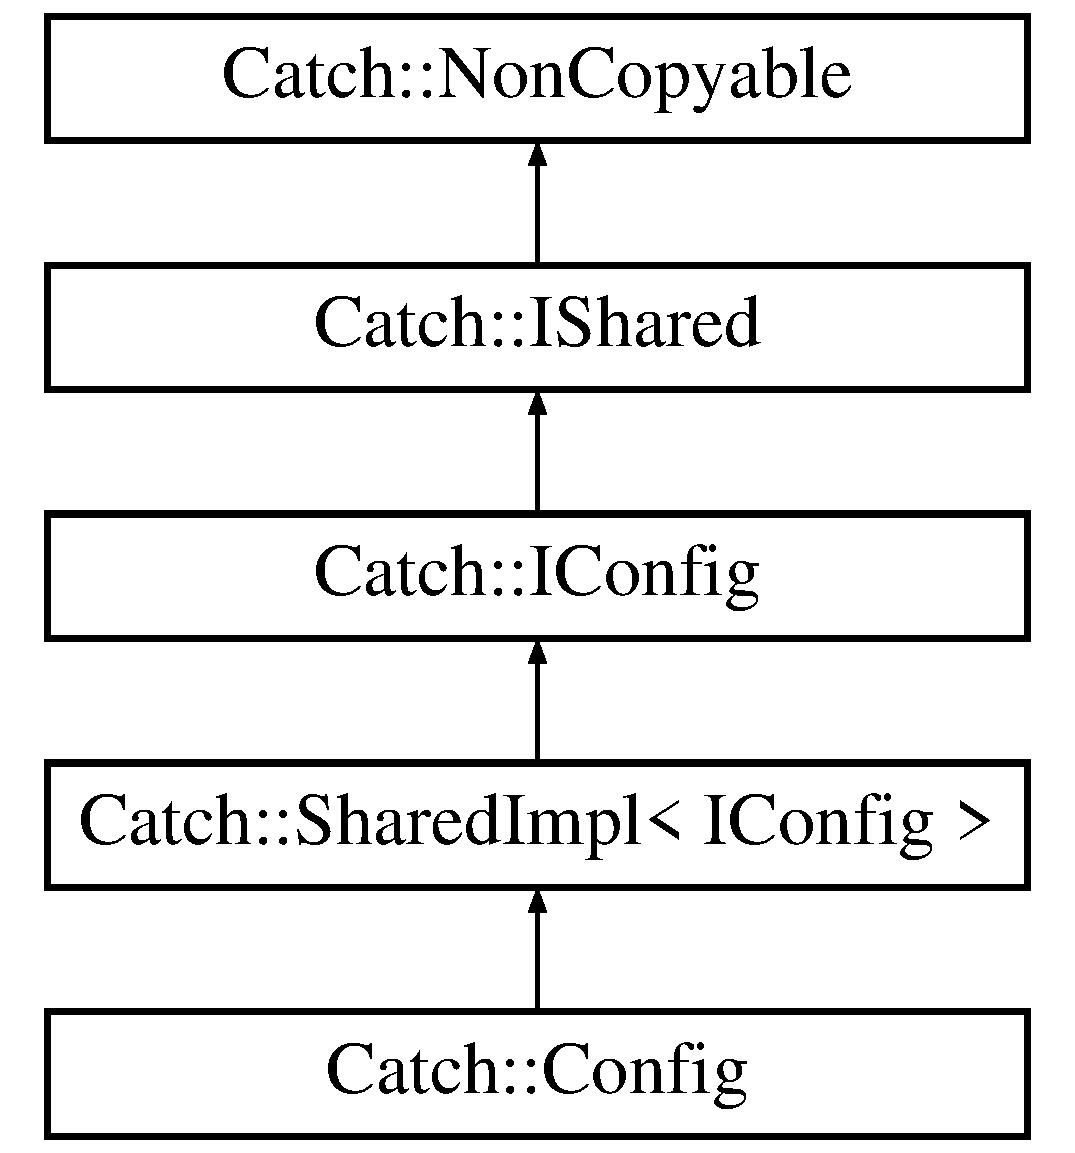
\includegraphics[height=5.000000cm]{class_catch_1_1_config}
\end{center}
\end{figure}
\subsection*{Public Member Functions}
\begin{DoxyCompactItemize}
\item 
\hypertarget{class_catch_1_1_config_a25ad0360a8386e7bc068c9c1ac5320bf}{{\bfseries Config} (\hyperlink{struct_catch_1_1_config_data}{Config\-Data} const \&data)}\label{class_catch_1_1_config_a25ad0360a8386e7bc068c9c1ac5320bf}

\item 
\hypertarget{class_catch_1_1_config_a08d869cec45133f75153a3e0f6095c71}{void {\bfseries set\-Filename} (std\-::string const \&filename)}\label{class_catch_1_1_config_a08d869cec45133f75153a3e0f6095c71}

\item 
\hypertarget{class_catch_1_1_config_aa9e256dae92ddb8502ff3680f8a5d87f}{std\-::string const \& {\bfseries get\-Filename} () const }\label{class_catch_1_1_config_aa9e256dae92ddb8502ff3680f8a5d87f}

\item 
\hypertarget{class_catch_1_1_config_aea015d29bfbe2518c4645ff0ea6d210e}{bool {\bfseries list\-Tests} () const }\label{class_catch_1_1_config_aea015d29bfbe2518c4645ff0ea6d210e}

\item 
\hypertarget{class_catch_1_1_config_a9dff59d5f71ce2d43719926d017e496e}{bool {\bfseries list\-Tags} () const }\label{class_catch_1_1_config_a9dff59d5f71ce2d43719926d017e496e}

\item 
\hypertarget{class_catch_1_1_config_a3107e37f61a84ca8914a107ecd1cb343}{bool {\bfseries list\-Reporters} () const }\label{class_catch_1_1_config_a3107e37f61a84ca8914a107ecd1cb343}

\item 
\hypertarget{class_catch_1_1_config_a7b0b80011521c7247f2365e213d0057c}{std\-::string {\bfseries get\-Process\-Name} () const }\label{class_catch_1_1_config_a7b0b80011521c7247f2365e213d0057c}

\item 
\hypertarget{class_catch_1_1_config_a404b40d7f51f3ee0955e737a4729a162}{bool {\bfseries should\-Debug\-Break} () const }\label{class_catch_1_1_config_a404b40d7f51f3ee0955e737a4729a162}

\item 
\hypertarget{class_catch_1_1_config_adacc2540c7876de06869ba56b14504da}{void {\bfseries set\-Stream\-Buf} (std\-::streambuf $\ast$buf)}\label{class_catch_1_1_config_adacc2540c7876de06869ba56b14504da}

\item 
\hypertarget{class_catch_1_1_config_ad54597f3f1f23f5a1cc862b5029bf231}{void {\bfseries use\-Stream} (std\-::string const \&stream\-Name)}\label{class_catch_1_1_config_ad54597f3f1f23f5a1cc862b5029bf231}

\item 
\hypertarget{class_catch_1_1_config_a6973175899892f42dd47a1d7701fbed7}{std\-::string {\bfseries get\-Reporter\-Name} () const }\label{class_catch_1_1_config_a6973175899892f42dd47a1d7701fbed7}

\item 
\hypertarget{class_catch_1_1_config_a50283ece0b30d1cd3c8e47588942232a}{void {\bfseries add\-Test\-Spec} (std\-::string const \&test\-Spec)}\label{class_catch_1_1_config_a50283ece0b30d1cd3c8e47588942232a}

\item 
\hypertarget{class_catch_1_1_config_a0ab98435c16d87681d370266b8755672}{int {\bfseries abort\-After} () const }\label{class_catch_1_1_config_a0ab98435c16d87681d370266b8755672}

\item 
\hypertarget{class_catch_1_1_config_ab91866ab6b895892ac29b4e9cfc1c1dd}{std\-::vector$<$ \hyperlink{class_catch_1_1_test_case_filters}{Test\-Case\-Filters} $>$\\*
 const \& {\bfseries filters} () const }\label{class_catch_1_1_config_ab91866ab6b895892ac29b4e9cfc1c1dd}

\item 
\hypertarget{class_catch_1_1_config_a338e89c6dd7c90d2772fc161cb77e9b4}{bool {\bfseries show\-Help} () const }\label{class_catch_1_1_config_a338e89c6dd7c90d2772fc161cb77e9b4}

\item 
\hypertarget{class_catch_1_1_config_ae6a5aea5e85afc2886b5ec8e3b610afa}{virtual bool {\bfseries allow\-Throws} () const }\label{class_catch_1_1_config_ae6a5aea5e85afc2886b5ec8e3b610afa}

\item 
\hypertarget{class_catch_1_1_config_a51a5f372698eaed4dd89c8bb03d2fdc4}{virtual std\-::ostream \& {\bfseries stream} () const }\label{class_catch_1_1_config_a51a5f372698eaed4dd89c8bb03d2fdc4}

\item 
\hypertarget{class_catch_1_1_config_a740c0195e2935033b71e3c3eaf0220c9}{virtual std\-::string {\bfseries name} () const }\label{class_catch_1_1_config_a740c0195e2935033b71e3c3eaf0220c9}

\item 
\hypertarget{class_catch_1_1_config_aea5f577057289ee2113cbe5adf296e69}{virtual bool {\bfseries include\-Successful\-Results} () const }\label{class_catch_1_1_config_aea5f577057289ee2113cbe5adf296e69}

\item 
\hypertarget{class_catch_1_1_config_ab8fdb451c6e214a24e8ff538ffaaa7e5}{virtual bool {\bfseries warn\-About\-Missing\-Assertions} () const }\label{class_catch_1_1_config_ab8fdb451c6e214a24e8ff538ffaaa7e5}

\item 
\hypertarget{class_catch_1_1_config_a192ff42482ade89d8225fcc0851909fd}{virtual Show\-Durations\-::\-Or\-Not {\bfseries show\-Durations} () const }\label{class_catch_1_1_config_a192ff42482ade89d8225fcc0851909fd}

\end{DoxyCompactItemize}
\subsection*{Additional Inherited Members}


The documentation for this class was generated from the following file\-:\begin{DoxyCompactItemize}
\item 
Catch.\-h\end{DoxyCompactItemize}

\hypertarget{struct_catch_1_1_config_data}{\section{Catch\-:\-:Config\-Data Struct Reference}
\label{struct_catch_1_1_config_data}\index{Catch\-::\-Config\-Data@{Catch\-::\-Config\-Data}}
}
\subsection*{Public Attributes}
\begin{DoxyCompactItemize}
\item 
\hypertarget{struct_catch_1_1_config_data_a0da0f6d493ef8f799273b4358d420a3a}{bool {\bfseries list\-Tests}}\label{struct_catch_1_1_config_data_a0da0f6d493ef8f799273b4358d420a3a}

\item 
\hypertarget{struct_catch_1_1_config_data_af780422bdef8d8b905204542855cf6b3}{bool {\bfseries list\-Tags}}\label{struct_catch_1_1_config_data_af780422bdef8d8b905204542855cf6b3}

\item 
\hypertarget{struct_catch_1_1_config_data_a4ba3618cae31b43237724f55359bfe95}{bool {\bfseries list\-Reporters}}\label{struct_catch_1_1_config_data_a4ba3618cae31b43237724f55359bfe95}

\item 
\hypertarget{struct_catch_1_1_config_data_aeb091ca2df2c654caaa2ad29c14578e5}{bool {\bfseries show\-Successful\-Tests}}\label{struct_catch_1_1_config_data_aeb091ca2df2c654caaa2ad29c14578e5}

\item 
\hypertarget{struct_catch_1_1_config_data_afec8310b1904784edb292e143a602fba}{bool {\bfseries should\-Debug\-Break}}\label{struct_catch_1_1_config_data_afec8310b1904784edb292e143a602fba}

\item 
\hypertarget{struct_catch_1_1_config_data_a6dd23f8c9d9337f46187e7dbb6a8328e}{bool {\bfseries no\-Throw}}\label{struct_catch_1_1_config_data_a6dd23f8c9d9337f46187e7dbb6a8328e}

\item 
\hypertarget{struct_catch_1_1_config_data_a12535241547dfc57e6864c4fc2cd4dd9}{bool {\bfseries show\-Help}}\label{struct_catch_1_1_config_data_a12535241547dfc57e6864c4fc2cd4dd9}

\item 
\hypertarget{struct_catch_1_1_config_data_a2d5505751aab745d5ae5e4ffe5c92c35}{int {\bfseries abort\-After}}\label{struct_catch_1_1_config_data_a2d5505751aab745d5ae5e4ffe5c92c35}

\item 
\hypertarget{struct_catch_1_1_config_data_ae274b251885569a6e1feba82f2cc9a31}{Verbosity\-::\-Level {\bfseries verbosity}}\label{struct_catch_1_1_config_data_ae274b251885569a6e1feba82f2cc9a31}

\item 
\hypertarget{struct_catch_1_1_config_data_af3a1c0b4a748b24799941b59bcd9c138}{Warn\-About\-::\-What {\bfseries warnings}}\label{struct_catch_1_1_config_data_af3a1c0b4a748b24799941b59bcd9c138}

\item 
\hypertarget{struct_catch_1_1_config_data_a26b02455c7cc772ab0be25af0ac12feb}{Show\-Durations\-::\-Or\-Not {\bfseries show\-Durations}}\label{struct_catch_1_1_config_data_a26b02455c7cc772ab0be25af0ac12feb}

\item 
\hypertarget{struct_catch_1_1_config_data_a86a1832b579b5b1728e3bd04dc03c35d}{std\-::string {\bfseries reporter\-Name}}\label{struct_catch_1_1_config_data_a86a1832b579b5b1728e3bd04dc03c35d}

\item 
\hypertarget{struct_catch_1_1_config_data_a6eaa8b628b7051824ac1717a5c2e8b5c}{std\-::string {\bfseries output\-Filename}}\label{struct_catch_1_1_config_data_a6eaa8b628b7051824ac1717a5c2e8b5c}

\item 
\hypertarget{struct_catch_1_1_config_data_a6c62e90478bc2911d032ec54c2e9d8df}{std\-::string {\bfseries name}}\label{struct_catch_1_1_config_data_a6c62e90478bc2911d032ec54c2e9d8df}

\item 
\hypertarget{struct_catch_1_1_config_data_ac181ec69c5b6c925ac9bea9eaf7039c3}{std\-::string {\bfseries process\-Name}}\label{struct_catch_1_1_config_data_ac181ec69c5b6c925ac9bea9eaf7039c3}

\item 
\hypertarget{struct_catch_1_1_config_data_aa40b0e5d2f78a7addbd5c8d16a111840}{std\-::vector$<$ std\-::string $>$ {\bfseries tests\-Or\-Tags}}\label{struct_catch_1_1_config_data_aa40b0e5d2f78a7addbd5c8d16a111840}

\end{DoxyCompactItemize}


The documentation for this struct was generated from the following file\-:\begin{DoxyCompactItemize}
\item 
Catch.\-h\end{DoxyCompactItemize}

\hypertarget{struct_catch_1_1_matchers_1_1_impl_1_1_std_string_1_1_contains}{\section{Catch\-:\-:Matchers\-:\-:Impl\-:\-:Std\-String\-:\-:Contains Struct Reference}
\label{struct_catch_1_1_matchers_1_1_impl_1_1_std_string_1_1_contains}\index{Catch\-::\-Matchers\-::\-Impl\-::\-Std\-String\-::\-Contains@{Catch\-::\-Matchers\-::\-Impl\-::\-Std\-String\-::\-Contains}}
}
Inheritance diagram for Catch\-:\-:Matchers\-:\-:Impl\-:\-:Std\-String\-:\-:Contains\-:\begin{figure}[H]
\begin{center}
\leavevmode
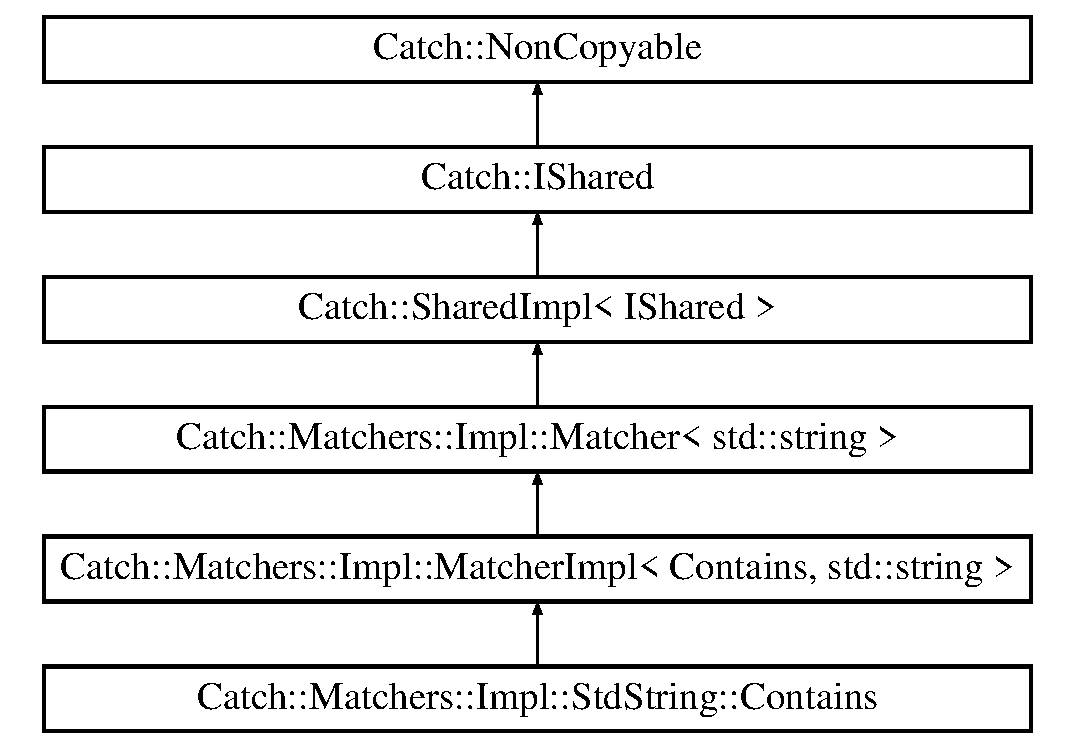
\includegraphics[height=6.000000cm]{struct_catch_1_1_matchers_1_1_impl_1_1_std_string_1_1_contains}
\end{center}
\end{figure}
\subsection*{Public Member Functions}
\begin{DoxyCompactItemize}
\item 
\hypertarget{struct_catch_1_1_matchers_1_1_impl_1_1_std_string_1_1_contains_ac6f13133724bfd5796e8ee4ea8f2c0e3}{{\bfseries Contains} (std\-::string const \&substr)}\label{struct_catch_1_1_matchers_1_1_impl_1_1_std_string_1_1_contains_ac6f13133724bfd5796e8ee4ea8f2c0e3}

\item 
\hypertarget{struct_catch_1_1_matchers_1_1_impl_1_1_std_string_1_1_contains_ad6b1ef653dfcb3bab43c43be043dc4e8}{{\bfseries Contains} (\hyperlink{struct_catch_1_1_matchers_1_1_impl_1_1_std_string_1_1_contains}{Contains} const \&other)}\label{struct_catch_1_1_matchers_1_1_impl_1_1_std_string_1_1_contains_ad6b1ef653dfcb3bab43c43be043dc4e8}

\item 
\hypertarget{struct_catch_1_1_matchers_1_1_impl_1_1_std_string_1_1_contains_aa27d823dea5770025a24424fc3355a6f}{virtual bool {\bfseries match} (std\-::string const \&expr) const }\label{struct_catch_1_1_matchers_1_1_impl_1_1_std_string_1_1_contains_aa27d823dea5770025a24424fc3355a6f}

\item 
\hypertarget{struct_catch_1_1_matchers_1_1_impl_1_1_std_string_1_1_contains_a226755351f3598179925f3ab89d6def7}{virtual std\-::string {\bfseries to\-String} () const }\label{struct_catch_1_1_matchers_1_1_impl_1_1_std_string_1_1_contains_a226755351f3598179925f3ab89d6def7}

\end{DoxyCompactItemize}
\subsection*{Public Attributes}
\begin{DoxyCompactItemize}
\item 
\hypertarget{struct_catch_1_1_matchers_1_1_impl_1_1_std_string_1_1_contains_a0bad82dd7cbdd0ec06b6d562181db03e}{std\-::string {\bfseries m\-\_\-substr}}\label{struct_catch_1_1_matchers_1_1_impl_1_1_std_string_1_1_contains_a0bad82dd7cbdd0ec06b6d562181db03e}

\end{DoxyCompactItemize}
\subsection*{Additional Inherited Members}


The documentation for this struct was generated from the following file\-:\begin{DoxyCompactItemize}
\item 
Catch.\-h\end{DoxyCompactItemize}

\hypertarget{struct_catch_1_1_counts}{\section{Catch\-:\-:Counts Struct Reference}
\label{struct_catch_1_1_counts}\index{Catch\-::\-Counts@{Catch\-::\-Counts}}
}
\subsection*{Public Member Functions}
\begin{DoxyCompactItemize}
\item 
\hypertarget{struct_catch_1_1_counts_aedf86fefe33938d132a6981171cd83e6}{\hyperlink{struct_catch_1_1_counts}{Counts} {\bfseries operator-\/} (\hyperlink{struct_catch_1_1_counts}{Counts} const \&other) const }\label{struct_catch_1_1_counts_aedf86fefe33938d132a6981171cd83e6}

\item 
\hypertarget{struct_catch_1_1_counts_a322a89475cd2cc039140ef371e973677}{\hyperlink{struct_catch_1_1_counts}{Counts} \& {\bfseries operator+=} (\hyperlink{struct_catch_1_1_counts}{Counts} const \&other)}\label{struct_catch_1_1_counts_a322a89475cd2cc039140ef371e973677}

\item 
\hypertarget{struct_catch_1_1_counts_a9125c662e30114e5c5cc94729b1e9e84}{std\-::size\-\_\-t {\bfseries total} () const }\label{struct_catch_1_1_counts_a9125c662e30114e5c5cc94729b1e9e84}

\end{DoxyCompactItemize}
\subsection*{Public Attributes}
\begin{DoxyCompactItemize}
\item 
\hypertarget{struct_catch_1_1_counts_ad28daaf3de28006400208b6dd0c631e6}{std\-::size\-\_\-t {\bfseries passed}}\label{struct_catch_1_1_counts_ad28daaf3de28006400208b6dd0c631e6}

\item 
\hypertarget{struct_catch_1_1_counts_a19982a3817a3bc2c07f0290e71f497a3}{std\-::size\-\_\-t {\bfseries failed}}\label{struct_catch_1_1_counts_a19982a3817a3bc2c07f0290e71f497a3}

\end{DoxyCompactItemize}


The documentation for this struct was generated from the following file\-:\begin{DoxyCompactItemize}
\item 
Catch.\-h\end{DoxyCompactItemize}

\hypertarget{struct_catch_1_1_cumulative_reporter_base}{\section{Catch\-:\-:Cumulative\-Reporter\-Base Struct Reference}
\label{struct_catch_1_1_cumulative_reporter_base}\index{Catch\-::\-Cumulative\-Reporter\-Base@{Catch\-::\-Cumulative\-Reporter\-Base}}
}
Inheritance diagram for Catch\-:\-:Cumulative\-Reporter\-Base\-:\begin{figure}[H]
\begin{center}
\leavevmode
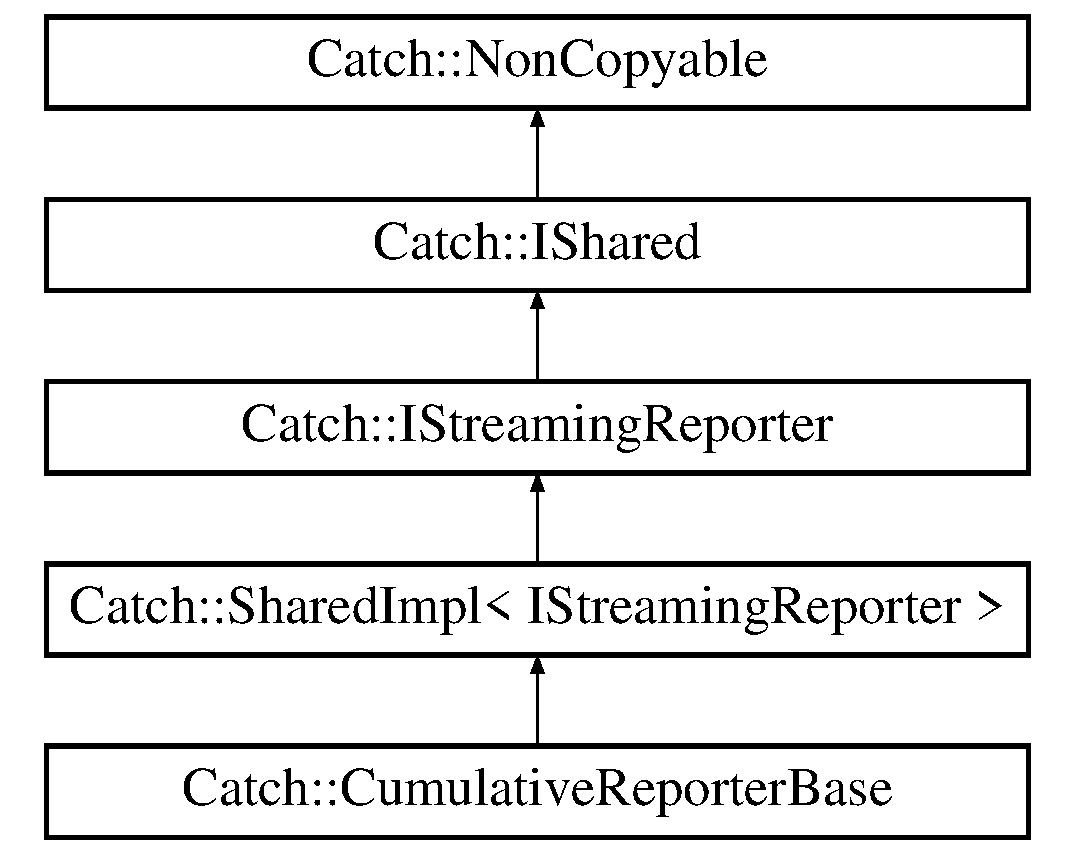
\includegraphics[height=5.000000cm]{struct_catch_1_1_cumulative_reporter_base}
\end{center}
\end{figure}
\subsection*{Classes}
\begin{DoxyCompactItemize}
\item 
struct \hyperlink{struct_catch_1_1_cumulative_reporter_base_1_1_node}{Node}
\item 
struct \hyperlink{struct_catch_1_1_cumulative_reporter_base_1_1_section_node}{Section\-Node}
\end{DoxyCompactItemize}
\subsection*{Public Types}
\begin{DoxyCompactItemize}
\item 
\hypertarget{struct_catch_1_1_cumulative_reporter_base_a46853912952f5286abbebfeba2266055}{typedef \hyperlink{struct_catch_1_1_cumulative_reporter_base_1_1_node}{Node}$<$ \hyperlink{struct_catch_1_1_test_case_stats}{Test\-Case\-Stats}, \\*
\hyperlink{struct_catch_1_1_cumulative_reporter_base_1_1_section_node}{Section\-Node} $>$ {\bfseries Test\-Case\-Node}}\label{struct_catch_1_1_cumulative_reporter_base_a46853912952f5286abbebfeba2266055}

\item 
\hypertarget{struct_catch_1_1_cumulative_reporter_base_a4c3fa5afc75155641d11f3aa01b97898}{typedef \hyperlink{struct_catch_1_1_cumulative_reporter_base_1_1_node}{Node}$<$ \hyperlink{struct_catch_1_1_test_group_stats}{Test\-Group\-Stats}, \\*
\hyperlink{struct_catch_1_1_cumulative_reporter_base_1_1_node}{Test\-Case\-Node} $>$ {\bfseries Test\-Group\-Node}}\label{struct_catch_1_1_cumulative_reporter_base_a4c3fa5afc75155641d11f3aa01b97898}

\item 
\hypertarget{struct_catch_1_1_cumulative_reporter_base_ac3f51b6d1942f4aa46afbb174f7265e6}{typedef \hyperlink{struct_catch_1_1_cumulative_reporter_base_1_1_node}{Node}$<$ \hyperlink{struct_catch_1_1_test_run_stats}{Test\-Run\-Stats}, \\*
\hyperlink{struct_catch_1_1_cumulative_reporter_base_1_1_node}{Test\-Group\-Node} $>$ {\bfseries Test\-Run\-Node}}\label{struct_catch_1_1_cumulative_reporter_base_ac3f51b6d1942f4aa46afbb174f7265e6}

\end{DoxyCompactItemize}
\subsection*{Public Member Functions}
\begin{DoxyCompactItemize}
\item 
\hypertarget{struct_catch_1_1_cumulative_reporter_base_ae25c7146268ae81fa0f944481d7ea5a5}{{\bfseries Cumulative\-Reporter\-Base} (\hyperlink{struct_catch_1_1_reporter_config}{Reporter\-Config} const \&\-\_\-config)}\label{struct_catch_1_1_cumulative_reporter_base_ae25c7146268ae81fa0f944481d7ea5a5}

\item 
\hypertarget{struct_catch_1_1_cumulative_reporter_base_a6326c26db277590f1d261953fd4b6733}{virtual void {\bfseries test\-Run\-Starting} (\hyperlink{struct_catch_1_1_test_run_info}{Test\-Run\-Info} const \&)}\label{struct_catch_1_1_cumulative_reporter_base_a6326c26db277590f1d261953fd4b6733}

\item 
\hypertarget{struct_catch_1_1_cumulative_reporter_base_a43f07792f2de8dce50ac0a24dbda6f5a}{virtual void {\bfseries test\-Group\-Starting} (\hyperlink{struct_catch_1_1_group_info}{Group\-Info} const \&)}\label{struct_catch_1_1_cumulative_reporter_base_a43f07792f2de8dce50ac0a24dbda6f5a}

\item 
\hypertarget{struct_catch_1_1_cumulative_reporter_base_affa61c6fb32e28a388afa45aa492c265}{virtual void {\bfseries test\-Case\-Starting} (\hyperlink{struct_catch_1_1_test_case_info}{Test\-Case\-Info} const \&)}\label{struct_catch_1_1_cumulative_reporter_base_affa61c6fb32e28a388afa45aa492c265}

\item 
\hypertarget{struct_catch_1_1_cumulative_reporter_base_a65bfe4710217c2d3eed5efe389adcd77}{virtual void {\bfseries section\-Starting} (\hyperlink{struct_catch_1_1_section_info}{Section\-Info} const \&section\-Info)}\label{struct_catch_1_1_cumulative_reporter_base_a65bfe4710217c2d3eed5efe389adcd77}

\item 
\hypertarget{struct_catch_1_1_cumulative_reporter_base_a7b5dfe0f0597083e686066ce7aeaaf35}{virtual void {\bfseries assertion\-Starting} (\hyperlink{struct_catch_1_1_assertion_info}{Assertion\-Info} const \&)}\label{struct_catch_1_1_cumulative_reporter_base_a7b5dfe0f0597083e686066ce7aeaaf35}

\item 
\hypertarget{struct_catch_1_1_cumulative_reporter_base_a22c7dfc613e911f97c621e436cde016c}{virtual bool {\bfseries assertion\-Ended} (\hyperlink{struct_catch_1_1_assertion_stats}{Assertion\-Stats} const \&assertion\-Stats)}\label{struct_catch_1_1_cumulative_reporter_base_a22c7dfc613e911f97c621e436cde016c}

\item 
\hypertarget{struct_catch_1_1_cumulative_reporter_base_a4d52c30f530df1ae55e44b09b5516f35}{virtual void {\bfseries section\-Ended} (\hyperlink{struct_catch_1_1_section_stats}{Section\-Stats} const \&section\-Stats)}\label{struct_catch_1_1_cumulative_reporter_base_a4d52c30f530df1ae55e44b09b5516f35}

\item 
\hypertarget{struct_catch_1_1_cumulative_reporter_base_af750cf4139005c09a0edc748919d5d60}{virtual void {\bfseries test\-Case\-Ended} (\hyperlink{struct_catch_1_1_test_case_stats}{Test\-Case\-Stats} const \&test\-Case\-Stats)}\label{struct_catch_1_1_cumulative_reporter_base_af750cf4139005c09a0edc748919d5d60}

\item 
\hypertarget{struct_catch_1_1_cumulative_reporter_base_a8a8072432ccbc7065d70493d68122bc5}{virtual void {\bfseries test\-Group\-Ended} (\hyperlink{struct_catch_1_1_test_group_stats}{Test\-Group\-Stats} const \&test\-Group\-Stats)}\label{struct_catch_1_1_cumulative_reporter_base_a8a8072432ccbc7065d70493d68122bc5}

\item 
\hypertarget{struct_catch_1_1_cumulative_reporter_base_ac4fa6adc0a7721e4f0094bd1f767cb2d}{virtual void {\bfseries test\-Run\-Ended} (\hyperlink{struct_catch_1_1_test_run_stats}{Test\-Run\-Stats} const \&test\-Run\-Stats)}\label{struct_catch_1_1_cumulative_reporter_base_ac4fa6adc0a7721e4f0094bd1f767cb2d}

\item 
\hypertarget{struct_catch_1_1_cumulative_reporter_base_a8c2077aad85caf632cbe2aad30e497a2}{virtual void {\bfseries test\-Run\-Ended} ()=0}\label{struct_catch_1_1_cumulative_reporter_base_a8c2077aad85caf632cbe2aad30e497a2}

\end{DoxyCompactItemize}
\subsection*{Public Attributes}
\begin{DoxyCompactItemize}
\item 
\hypertarget{struct_catch_1_1_cumulative_reporter_base_a19a52c03908bdc2f781a99d844f07c8e}{\hyperlink{class_catch_1_1_ptr}{Ptr}$<$ \hyperlink{struct_catch_1_1_i_config}{I\-Config} $>$ {\bfseries m\-\_\-config}}\label{struct_catch_1_1_cumulative_reporter_base_a19a52c03908bdc2f781a99d844f07c8e}

\item 
\hypertarget{struct_catch_1_1_cumulative_reporter_base_add96a41a3e449be82c629a9cefc84aac}{std\-::ostream \& {\bfseries stream}}\label{struct_catch_1_1_cumulative_reporter_base_add96a41a3e449be82c629a9cefc84aac}

\item 
\hypertarget{struct_catch_1_1_cumulative_reporter_base_acb33a9784c0e8c0b8d477dff96ed36cb}{std\-::vector$<$ \hyperlink{struct_catch_1_1_assertion_stats}{Assertion\-Stats} $>$ {\bfseries m\-\_\-assertions}}\label{struct_catch_1_1_cumulative_reporter_base_acb33a9784c0e8c0b8d477dff96ed36cb}

\item 
\hypertarget{struct_catch_1_1_cumulative_reporter_base_ad88d6066ef6c5ef1f02f64a41672d259}{std\-::vector$<$ std\-::vector$<$ \hyperlink{class_catch_1_1_ptr}{Ptr}\\*
$<$ \hyperlink{struct_catch_1_1_cumulative_reporter_base_1_1_section_node}{Section\-Node} $>$ $>$ $>$ {\bfseries m\-\_\-sections}}\label{struct_catch_1_1_cumulative_reporter_base_ad88d6066ef6c5ef1f02f64a41672d259}

\item 
\hypertarget{struct_catch_1_1_cumulative_reporter_base_aabb351de73df367d80ec12734997448c}{std\-::vector$<$ \hyperlink{class_catch_1_1_ptr}{Ptr}$<$ \hyperlink{struct_catch_1_1_cumulative_reporter_base_1_1_node}{Test\-Case\-Node} $>$ $>$ {\bfseries m\-\_\-test\-Cases}}\label{struct_catch_1_1_cumulative_reporter_base_aabb351de73df367d80ec12734997448c}

\item 
\hypertarget{struct_catch_1_1_cumulative_reporter_base_a39db5cc0dc6646aa42f20b2b981b9ae5}{std\-::vector$<$ \hyperlink{class_catch_1_1_ptr}{Ptr}$<$ \hyperlink{struct_catch_1_1_cumulative_reporter_base_1_1_node}{Test\-Group\-Node} $>$ $>$ {\bfseries m\-\_\-test\-Groups}}\label{struct_catch_1_1_cumulative_reporter_base_a39db5cc0dc6646aa42f20b2b981b9ae5}

\item 
\hypertarget{struct_catch_1_1_cumulative_reporter_base_abbcd7bb9f8ec2dff8520c2d04df1e6ce}{std\-::vector$<$ \hyperlink{class_catch_1_1_ptr}{Ptr}$<$ \hyperlink{struct_catch_1_1_cumulative_reporter_base_1_1_node}{Test\-Run\-Node} $>$ $>$ {\bfseries m\-\_\-test\-Runs}}\label{struct_catch_1_1_cumulative_reporter_base_abbcd7bb9f8ec2dff8520c2d04df1e6ce}

\item 
\hypertarget{struct_catch_1_1_cumulative_reporter_base_a407c1ad0723f3e10efbb982c5adbd07c}{\hyperlink{class_catch_1_1_ptr}{Ptr}$<$ \hyperlink{struct_catch_1_1_cumulative_reporter_base_1_1_section_node}{Section\-Node} $>$ {\bfseries m\-\_\-root\-Section}}\label{struct_catch_1_1_cumulative_reporter_base_a407c1ad0723f3e10efbb982c5adbd07c}

\item 
\hypertarget{struct_catch_1_1_cumulative_reporter_base_a9058ef2fc03d698503fccd918c64d0f2}{\hyperlink{class_catch_1_1_ptr}{Ptr}$<$ \hyperlink{struct_catch_1_1_cumulative_reporter_base_1_1_section_node}{Section\-Node} $>$ {\bfseries m\-\_\-deepest\-Section}}\label{struct_catch_1_1_cumulative_reporter_base_a9058ef2fc03d698503fccd918c64d0f2}

\item 
\hypertarget{struct_catch_1_1_cumulative_reporter_base_ae64972fbf6026c4f72ebbc9c0b1c9d41}{std\-::vector$<$ \hyperlink{class_catch_1_1_ptr}{Ptr}$<$ \hyperlink{struct_catch_1_1_cumulative_reporter_base_1_1_section_node}{Section\-Node} $>$ $>$ {\bfseries m\-\_\-section\-Stack}}\label{struct_catch_1_1_cumulative_reporter_base_ae64972fbf6026c4f72ebbc9c0b1c9d41}

\end{DoxyCompactItemize}
\subsection*{Friends}
\begin{DoxyCompactItemize}
\item 
\hypertarget{struct_catch_1_1_cumulative_reporter_base_a8a9f836c62348333bde04b059851b738}{bool {\bfseries operator==} (\hyperlink{class_catch_1_1_ptr}{Ptr}$<$ \hyperlink{struct_catch_1_1_cumulative_reporter_base_1_1_section_node}{Section\-Node} $>$ const \&node, \hyperlink{struct_catch_1_1_section_info}{Section\-Info} const \&other)}\label{struct_catch_1_1_cumulative_reporter_base_a8a9f836c62348333bde04b059851b738}

\end{DoxyCompactItemize}


The documentation for this struct was generated from the following file\-:\begin{DoxyCompactItemize}
\item 
Catch.\-h\end{DoxyCompactItemize}

\hypertarget{struct_catch_1_1_matchers_1_1_impl_1_1_std_string_1_1_ends_with}{\section{Catch\-:\-:Matchers\-:\-:Impl\-:\-:Std\-String\-:\-:Ends\-With Struct Reference}
\label{struct_catch_1_1_matchers_1_1_impl_1_1_std_string_1_1_ends_with}\index{Catch\-::\-Matchers\-::\-Impl\-::\-Std\-String\-::\-Ends\-With@{Catch\-::\-Matchers\-::\-Impl\-::\-Std\-String\-::\-Ends\-With}}
}
Inheritance diagram for Catch\-:\-:Matchers\-:\-:Impl\-:\-:Std\-String\-:\-:Ends\-With\-:\begin{figure}[H]
\begin{center}
\leavevmode
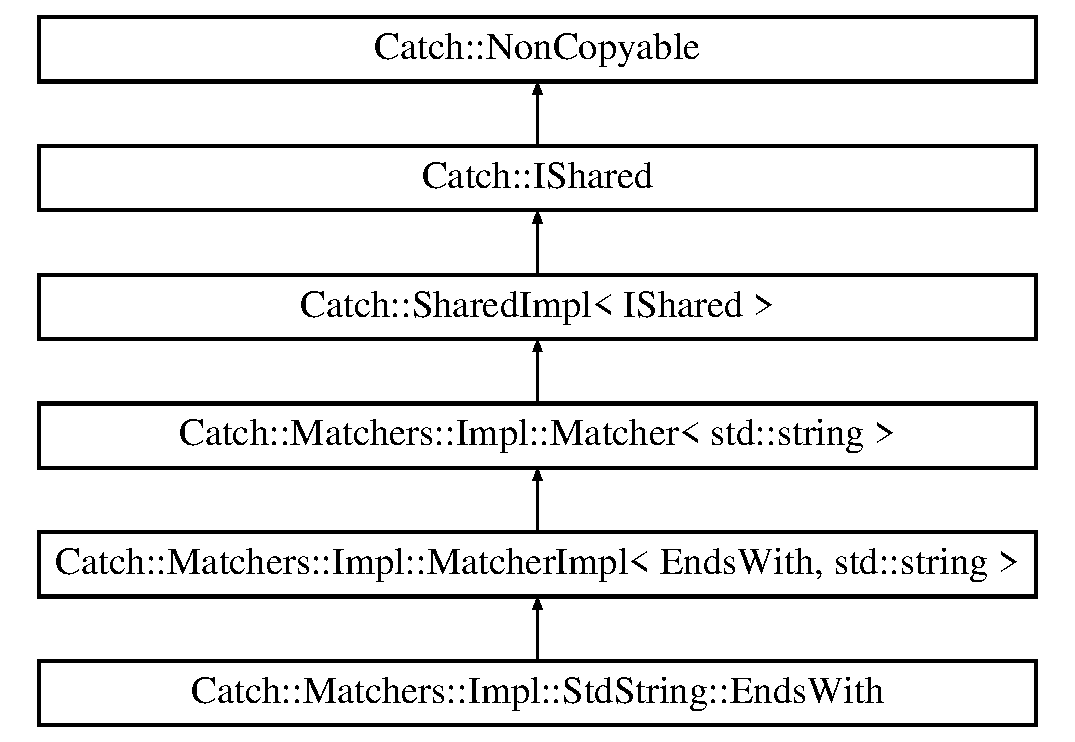
\includegraphics[height=6.000000cm]{struct_catch_1_1_matchers_1_1_impl_1_1_std_string_1_1_ends_with}
\end{center}
\end{figure}
\subsection*{Public Member Functions}
\begin{DoxyCompactItemize}
\item 
\hypertarget{struct_catch_1_1_matchers_1_1_impl_1_1_std_string_1_1_ends_with_a82730175f7f7475ce1ee9791e160d02d}{{\bfseries Ends\-With} (std\-::string const \&substr)}\label{struct_catch_1_1_matchers_1_1_impl_1_1_std_string_1_1_ends_with_a82730175f7f7475ce1ee9791e160d02d}

\item 
\hypertarget{struct_catch_1_1_matchers_1_1_impl_1_1_std_string_1_1_ends_with_a9321aac07fb17613a7993e99003b3be2}{{\bfseries Ends\-With} (\hyperlink{struct_catch_1_1_matchers_1_1_impl_1_1_std_string_1_1_ends_with}{Ends\-With} const \&other)}\label{struct_catch_1_1_matchers_1_1_impl_1_1_std_string_1_1_ends_with_a9321aac07fb17613a7993e99003b3be2}

\item 
\hypertarget{struct_catch_1_1_matchers_1_1_impl_1_1_std_string_1_1_ends_with_ad0e03d7f54ffa5859f84faebccf11e76}{virtual bool {\bfseries match} (std\-::string const \&expr) const }\label{struct_catch_1_1_matchers_1_1_impl_1_1_std_string_1_1_ends_with_ad0e03d7f54ffa5859f84faebccf11e76}

\item 
\hypertarget{struct_catch_1_1_matchers_1_1_impl_1_1_std_string_1_1_ends_with_a54715c94c215a1fc5fb6336acf52eb06}{virtual std\-::string {\bfseries to\-String} () const }\label{struct_catch_1_1_matchers_1_1_impl_1_1_std_string_1_1_ends_with_a54715c94c215a1fc5fb6336acf52eb06}

\end{DoxyCompactItemize}
\subsection*{Public Attributes}
\begin{DoxyCompactItemize}
\item 
\hypertarget{struct_catch_1_1_matchers_1_1_impl_1_1_std_string_1_1_ends_with_a5abf70e94ea7893b7bd1e7b33880ba7b}{std\-::string {\bfseries m\-\_\-substr}}\label{struct_catch_1_1_matchers_1_1_impl_1_1_std_string_1_1_ends_with_a5abf70e94ea7893b7bd1e7b33880ba7b}

\end{DoxyCompactItemize}
\subsection*{Additional Inherited Members}


The documentation for this struct was generated from the following file\-:\begin{DoxyCompactItemize}
\item 
Catch.\-h\end{DoxyCompactItemize}

\hypertarget{struct_catch_1_1_matchers_1_1_impl_1_1_std_string_1_1_equals}{\section{Catch\-:\-:Matchers\-:\-:Impl\-:\-:Std\-String\-:\-:Equals Struct Reference}
\label{struct_catch_1_1_matchers_1_1_impl_1_1_std_string_1_1_equals}\index{Catch\-::\-Matchers\-::\-Impl\-::\-Std\-String\-::\-Equals@{Catch\-::\-Matchers\-::\-Impl\-::\-Std\-String\-::\-Equals}}
}
Inheritance diagram for Catch\-:\-:Matchers\-:\-:Impl\-:\-:Std\-String\-:\-:Equals\-:\begin{figure}[H]
\begin{center}
\leavevmode
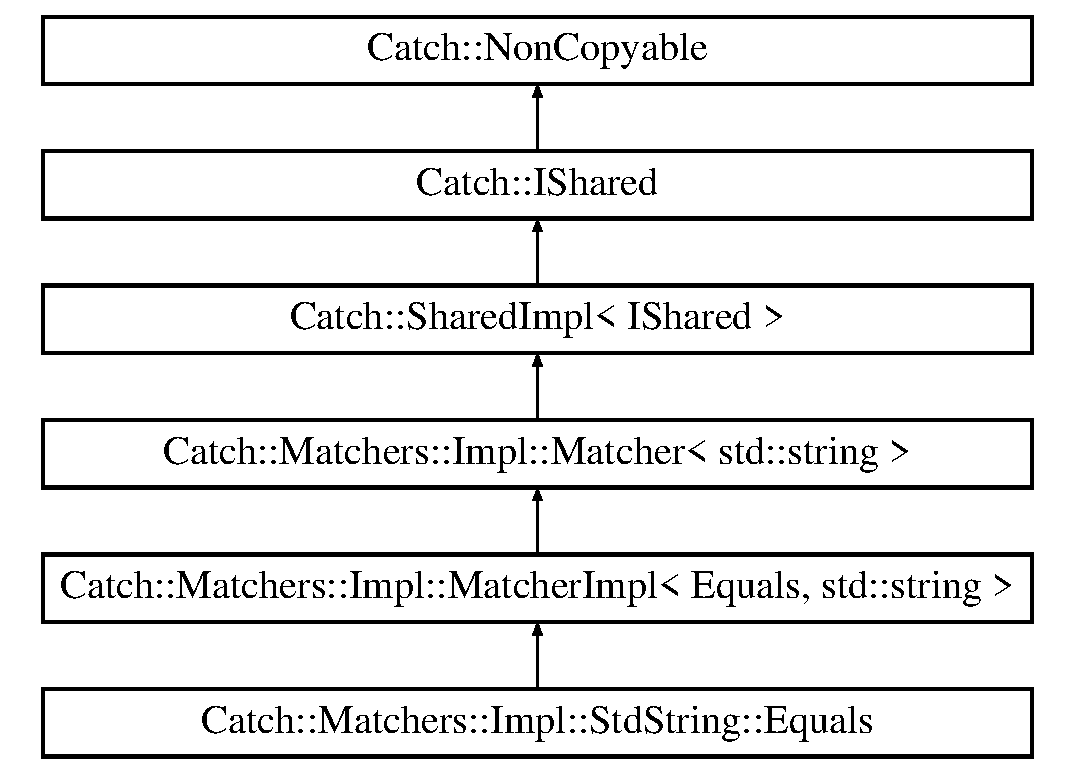
\includegraphics[height=6.000000cm]{struct_catch_1_1_matchers_1_1_impl_1_1_std_string_1_1_equals}
\end{center}
\end{figure}
\subsection*{Public Member Functions}
\begin{DoxyCompactItemize}
\item 
\hypertarget{struct_catch_1_1_matchers_1_1_impl_1_1_std_string_1_1_equals_a1bd99b381c6116a02b1e3ca200ca920c}{{\bfseries Equals} (std\-::string const \&str)}\label{struct_catch_1_1_matchers_1_1_impl_1_1_std_string_1_1_equals_a1bd99b381c6116a02b1e3ca200ca920c}

\item 
\hypertarget{struct_catch_1_1_matchers_1_1_impl_1_1_std_string_1_1_equals_acaa97de06aedf363ae803d65a975f5e4}{{\bfseries Equals} (\hyperlink{struct_catch_1_1_matchers_1_1_impl_1_1_std_string_1_1_equals}{Equals} const \&other)}\label{struct_catch_1_1_matchers_1_1_impl_1_1_std_string_1_1_equals_acaa97de06aedf363ae803d65a975f5e4}

\item 
\hypertarget{struct_catch_1_1_matchers_1_1_impl_1_1_std_string_1_1_equals_a00c8259a76c24da669e116662ededc70}{virtual bool {\bfseries match} (std\-::string const \&expr) const }\label{struct_catch_1_1_matchers_1_1_impl_1_1_std_string_1_1_equals_a00c8259a76c24da669e116662ededc70}

\item 
\hypertarget{struct_catch_1_1_matchers_1_1_impl_1_1_std_string_1_1_equals_a7a09449ff2f858981caf3b1f6c36d270}{virtual std\-::string {\bfseries to\-String} () const }\label{struct_catch_1_1_matchers_1_1_impl_1_1_std_string_1_1_equals_a7a09449ff2f858981caf3b1f6c36d270}

\end{DoxyCompactItemize}
\subsection*{Public Attributes}
\begin{DoxyCompactItemize}
\item 
\hypertarget{struct_catch_1_1_matchers_1_1_impl_1_1_std_string_1_1_equals_a41fc4413185f47d8b6d8da7a55078921}{std\-::string {\bfseries m\-\_\-str}}\label{struct_catch_1_1_matchers_1_1_impl_1_1_std_string_1_1_equals_a41fc4413185f47d8b6d8da7a55078921}

\end{DoxyCompactItemize}
\subsection*{Additional Inherited Members}


The documentation for this struct was generated from the following file\-:\begin{DoxyCompactItemize}
\item 
Catch.\-h\end{DoxyCompactItemize}

\hypertarget{class_catch_1_1_internal_1_1_evaluator}{\section{Catch\-:\-:Internal\-:\-:Evaluator$<$ T1, T2, Op $>$ Class Template Reference}
\label{class_catch_1_1_internal_1_1_evaluator}\index{Catch\-::\-Internal\-::\-Evaluator$<$ T1, T2, Op $>$@{Catch\-::\-Internal\-::\-Evaluator$<$ T1, T2, Op $>$}}
}


The documentation for this class was generated from the following file\-:\begin{DoxyCompactItemize}
\item 
Catch.\-h\end{DoxyCompactItemize}

\hypertarget{struct_catch_1_1_internal_1_1_evaluator_3_01_t1_00_01_t2_00_01_is_equal_to_01_4}{\section{Catch\-:\-:Internal\-:\-:Evaluator$<$ T1, T2, Is\-Equal\-To $>$ Struct Template Reference}
\label{struct_catch_1_1_internal_1_1_evaluator_3_01_t1_00_01_t2_00_01_is_equal_to_01_4}\index{Catch\-::\-Internal\-::\-Evaluator$<$ T1, T2, Is\-Equal\-To $>$@{Catch\-::\-Internal\-::\-Evaluator$<$ T1, T2, Is\-Equal\-To $>$}}
}
\subsection*{Static Public Member Functions}
\begin{DoxyCompactItemize}
\item 
\hypertarget{struct_catch_1_1_internal_1_1_evaluator_3_01_t1_00_01_t2_00_01_is_equal_to_01_4_a166b2b7849247397e63fb2940481b217}{static bool {\bfseries evaluate} (T1 const \&lhs, T2 const \&rhs)}\label{struct_catch_1_1_internal_1_1_evaluator_3_01_t1_00_01_t2_00_01_is_equal_to_01_4_a166b2b7849247397e63fb2940481b217}

\end{DoxyCompactItemize}


The documentation for this struct was generated from the following file\-:\begin{DoxyCompactItemize}
\item 
Catch.\-h\end{DoxyCompactItemize}

\hypertarget{struct_catch_1_1_internal_1_1_evaluator_3_01_t1_00_01_t2_00_01_is_greater_than_01_4}{\section{Catch\-:\-:Internal\-:\-:Evaluator$<$ T1, T2, Is\-Greater\-Than $>$ Struct Template Reference}
\label{struct_catch_1_1_internal_1_1_evaluator_3_01_t1_00_01_t2_00_01_is_greater_than_01_4}\index{Catch\-::\-Internal\-::\-Evaluator$<$ T1, T2, Is\-Greater\-Than $>$@{Catch\-::\-Internal\-::\-Evaluator$<$ T1, T2, Is\-Greater\-Than $>$}}
}
\subsection*{Static Public Member Functions}
\begin{DoxyCompactItemize}
\item 
\hypertarget{struct_catch_1_1_internal_1_1_evaluator_3_01_t1_00_01_t2_00_01_is_greater_than_01_4_a55745f74f09ac5c61bd3d592ca5560af}{static bool {\bfseries evaluate} (T1 const \&lhs, T2 const \&rhs)}\label{struct_catch_1_1_internal_1_1_evaluator_3_01_t1_00_01_t2_00_01_is_greater_than_01_4_a55745f74f09ac5c61bd3d592ca5560af}

\end{DoxyCompactItemize}


The documentation for this struct was generated from the following file\-:\begin{DoxyCompactItemize}
\item 
Catch.\-h\end{DoxyCompactItemize}

\hypertarget{struct_catch_1_1_internal_1_1_evaluator_3_01_t1_00_01_t2_00_01_is_greater_than_or_equal_to_01_4}{\section{Catch\-:\-:Internal\-:\-:Evaluator$<$ T1, T2, Is\-Greater\-Than\-Or\-Equal\-To $>$ Struct Template Reference}
\label{struct_catch_1_1_internal_1_1_evaluator_3_01_t1_00_01_t2_00_01_is_greater_than_or_equal_to_01_4}\index{Catch\-::\-Internal\-::\-Evaluator$<$ T1, T2, Is\-Greater\-Than\-Or\-Equal\-To $>$@{Catch\-::\-Internal\-::\-Evaluator$<$ T1, T2, Is\-Greater\-Than\-Or\-Equal\-To $>$}}
}
\subsection*{Static Public Member Functions}
\begin{DoxyCompactItemize}
\item 
\hypertarget{struct_catch_1_1_internal_1_1_evaluator_3_01_t1_00_01_t2_00_01_is_greater_than_or_equal_to_01_4_a5ba107c6da4292b6492a0e5e906f9484}{static bool {\bfseries evaluate} (T1 const \&lhs, T2 const \&rhs)}\label{struct_catch_1_1_internal_1_1_evaluator_3_01_t1_00_01_t2_00_01_is_greater_than_or_equal_to_01_4_a5ba107c6da4292b6492a0e5e906f9484}

\end{DoxyCompactItemize}


The documentation for this struct was generated from the following file\-:\begin{DoxyCompactItemize}
\item 
Catch.\-h\end{DoxyCompactItemize}

\hypertarget{struct_catch_1_1_internal_1_1_evaluator_3_01_t1_00_01_t2_00_01_is_less_than_01_4}{\section{Catch\-:\-:Internal\-:\-:Evaluator$<$ T1, T2, Is\-Less\-Than $>$ Struct Template Reference}
\label{struct_catch_1_1_internal_1_1_evaluator_3_01_t1_00_01_t2_00_01_is_less_than_01_4}\index{Catch\-::\-Internal\-::\-Evaluator$<$ T1, T2, Is\-Less\-Than $>$@{Catch\-::\-Internal\-::\-Evaluator$<$ T1, T2, Is\-Less\-Than $>$}}
}
\subsection*{Static Public Member Functions}
\begin{DoxyCompactItemize}
\item 
\hypertarget{struct_catch_1_1_internal_1_1_evaluator_3_01_t1_00_01_t2_00_01_is_less_than_01_4_a75b2bcf80ce6f90218c145e2c3293d75}{static bool {\bfseries evaluate} (T1 const \&lhs, T2 const \&rhs)}\label{struct_catch_1_1_internal_1_1_evaluator_3_01_t1_00_01_t2_00_01_is_less_than_01_4_a75b2bcf80ce6f90218c145e2c3293d75}

\end{DoxyCompactItemize}


The documentation for this struct was generated from the following file\-:\begin{DoxyCompactItemize}
\item 
Catch.\-h\end{DoxyCompactItemize}

\hypertarget{struct_catch_1_1_internal_1_1_evaluator_3_01_t1_00_01_t2_00_01_is_less_than_or_equal_to_01_4}{\section{Catch\-:\-:Internal\-:\-:Evaluator$<$ T1, T2, Is\-Less\-Than\-Or\-Equal\-To $>$ Struct Template Reference}
\label{struct_catch_1_1_internal_1_1_evaluator_3_01_t1_00_01_t2_00_01_is_less_than_or_equal_to_01_4}\index{Catch\-::\-Internal\-::\-Evaluator$<$ T1, T2, Is\-Less\-Than\-Or\-Equal\-To $>$@{Catch\-::\-Internal\-::\-Evaluator$<$ T1, T2, Is\-Less\-Than\-Or\-Equal\-To $>$}}
}
\subsection*{Static Public Member Functions}
\begin{DoxyCompactItemize}
\item 
\hypertarget{struct_catch_1_1_internal_1_1_evaluator_3_01_t1_00_01_t2_00_01_is_less_than_or_equal_to_01_4_adf269a597e4d82d69f29bcb516297b9b}{static bool {\bfseries evaluate} (T1 const \&lhs, T2 const \&rhs)}\label{struct_catch_1_1_internal_1_1_evaluator_3_01_t1_00_01_t2_00_01_is_less_than_or_equal_to_01_4_adf269a597e4d82d69f29bcb516297b9b}

\end{DoxyCompactItemize}


The documentation for this struct was generated from the following file\-:\begin{DoxyCompactItemize}
\item 
Catch.\-h\end{DoxyCompactItemize}

\hypertarget{struct_catch_1_1_internal_1_1_evaluator_3_01_t1_00_01_t2_00_01_is_not_equal_to_01_4}{\section{Catch\-:\-:Internal\-:\-:Evaluator$<$ T1, T2, Is\-Not\-Equal\-To $>$ Struct Template Reference}
\label{struct_catch_1_1_internal_1_1_evaluator_3_01_t1_00_01_t2_00_01_is_not_equal_to_01_4}\index{Catch\-::\-Internal\-::\-Evaluator$<$ T1, T2, Is\-Not\-Equal\-To $>$@{Catch\-::\-Internal\-::\-Evaluator$<$ T1, T2, Is\-Not\-Equal\-To $>$}}
}
\subsection*{Static Public Member Functions}
\begin{DoxyCompactItemize}
\item 
\hypertarget{struct_catch_1_1_internal_1_1_evaluator_3_01_t1_00_01_t2_00_01_is_not_equal_to_01_4_a956a12d0f4a7dceb5a1ce914421ff945}{static bool {\bfseries evaluate} (T1 const \&lhs, T2 const \&rhs)}\label{struct_catch_1_1_internal_1_1_evaluator_3_01_t1_00_01_t2_00_01_is_not_equal_to_01_4_a956a12d0f4a7dceb5a1ce914421ff945}

\end{DoxyCompactItemize}


The documentation for this struct was generated from the following file\-:\begin{DoxyCompactItemize}
\item 
Catch.\-h\end{DoxyCompactItemize}

\hypertarget{class_catch_1_1_exception_translator_registrar}{\section{Catch\-:\-:Exception\-Translator\-Registrar Class Reference}
\label{class_catch_1_1_exception_translator_registrar}\index{Catch\-::\-Exception\-Translator\-Registrar@{Catch\-::\-Exception\-Translator\-Registrar}}
}
\subsection*{Public Member Functions}
\begin{DoxyCompactItemize}
\item 
\hypertarget{class_catch_1_1_exception_translator_registrar_aa73229de911f26b1df6c6c87c4d9e04e}{{\footnotesize template$<$typename T $>$ }\\{\bfseries Exception\-Translator\-Registrar} (std\-::string($\ast$translate\-Function)(T \&))}\label{class_catch_1_1_exception_translator_registrar_aa73229de911f26b1df6c6c87c4d9e04e}

\end{DoxyCompactItemize}


The documentation for this class was generated from the following file\-:\begin{DoxyCompactItemize}
\item 
Catch.\-h\end{DoxyCompactItemize}

\hypertarget{class_catch_1_1_expression_decomposer}{\section{Catch\-:\-:Expression\-Decomposer Class Reference}
\label{class_catch_1_1_expression_decomposer}\index{Catch\-::\-Expression\-Decomposer@{Catch\-::\-Expression\-Decomposer}}
}
\subsection*{Public Member Functions}
\begin{DoxyCompactItemize}
\item 
\hypertarget{class_catch_1_1_expression_decomposer_a22496794d8f55e571ff719516eba4d49}{{\footnotesize template$<$typename T $>$ }\\\hyperlink{class_catch_1_1_expression_lhs}{Expression\-Lhs}$<$ T const \& $>$ {\bfseries operator-\/$>$$\ast$} (T const \&operand)}\label{class_catch_1_1_expression_decomposer_a22496794d8f55e571ff719516eba4d49}

\item 
\hypertarget{class_catch_1_1_expression_decomposer_afd4a9fca08154c361ea2a144a244be18}{\hyperlink{class_catch_1_1_expression_lhs}{Expression\-Lhs}$<$ bool $>$ {\bfseries operator-\/$>$$\ast$} (bool value)}\label{class_catch_1_1_expression_decomposer_afd4a9fca08154c361ea2a144a244be18}

\end{DoxyCompactItemize}


The documentation for this class was generated from the following file\-:\begin{DoxyCompactItemize}
\item 
Catch.\-h\end{DoxyCompactItemize}

\hypertarget{class_catch_1_1_expression_lhs}{\section{Catch\-:\-:Expression\-Lhs$<$ T $>$ Class Template Reference}
\label{class_catch_1_1_expression_lhs}\index{Catch\-::\-Expression\-Lhs$<$ T $>$@{Catch\-::\-Expression\-Lhs$<$ T $>$}}
}
\subsection*{Public Member Functions}
\begin{DoxyCompactItemize}
\item 
\hypertarget{class_catch_1_1_expression_lhs_a22d67f6de8fd701f82ca0c91fc3a381d}{{\bfseries Expression\-Lhs} (T lhs)}\label{class_catch_1_1_expression_lhs_a22d67f6de8fd701f82ca0c91fc3a381d}

\item 
\hypertarget{class_catch_1_1_expression_lhs_ad6247606e88d1d188b0736d07c7cfc1a}{{\footnotesize template$<$typename Rhs\-T $>$ }\\\hyperlink{class_catch_1_1_expression_result_builder}{Expression\-Result\-Builder} \& {\bfseries operator==} (Rhs\-T const \&rhs)}\label{class_catch_1_1_expression_lhs_ad6247606e88d1d188b0736d07c7cfc1a}

\item 
\hypertarget{class_catch_1_1_expression_lhs_a27dc38036186c11f7c197ea3ebb20530}{{\footnotesize template$<$typename Rhs\-T $>$ }\\\hyperlink{class_catch_1_1_expression_result_builder}{Expression\-Result\-Builder} \& {\bfseries operator!=} (Rhs\-T const \&rhs)}\label{class_catch_1_1_expression_lhs_a27dc38036186c11f7c197ea3ebb20530}

\item 
\hypertarget{class_catch_1_1_expression_lhs_aff8d8124d948895897c4f2d52d39d8df}{{\footnotesize template$<$typename Rhs\-T $>$ }\\\hyperlink{class_catch_1_1_expression_result_builder}{Expression\-Result\-Builder} \& {\bfseries operator$<$} (Rhs\-T const \&rhs)}\label{class_catch_1_1_expression_lhs_aff8d8124d948895897c4f2d52d39d8df}

\item 
\hypertarget{class_catch_1_1_expression_lhs_a831eaabf3e182c8f36eede97182e513d}{{\footnotesize template$<$typename Rhs\-T $>$ }\\\hyperlink{class_catch_1_1_expression_result_builder}{Expression\-Result\-Builder} \& {\bfseries operator$>$} (Rhs\-T const \&rhs)}\label{class_catch_1_1_expression_lhs_a831eaabf3e182c8f36eede97182e513d}

\item 
\hypertarget{class_catch_1_1_expression_lhs_a6d43fbf5741cae70b1908ed75ac19784}{{\footnotesize template$<$typename Rhs\-T $>$ }\\\hyperlink{class_catch_1_1_expression_result_builder}{Expression\-Result\-Builder} \& {\bfseries operator$<$=} (Rhs\-T const \&rhs)}\label{class_catch_1_1_expression_lhs_a6d43fbf5741cae70b1908ed75ac19784}

\item 
\hypertarget{class_catch_1_1_expression_lhs_ae197c4a4d3fb35e01ede684c6e75115f}{{\footnotesize template$<$typename Rhs\-T $>$ }\\\hyperlink{class_catch_1_1_expression_result_builder}{Expression\-Result\-Builder} \& {\bfseries operator$>$=} (Rhs\-T const \&rhs)}\label{class_catch_1_1_expression_lhs_ae197c4a4d3fb35e01ede684c6e75115f}

\item 
\hypertarget{class_catch_1_1_expression_lhs_a11906256509e816eb51eff3e24154d47}{\hyperlink{class_catch_1_1_expression_result_builder}{Expression\-Result\-Builder} \& {\bfseries operator==} (bool rhs)}\label{class_catch_1_1_expression_lhs_a11906256509e816eb51eff3e24154d47}

\item 
\hypertarget{class_catch_1_1_expression_lhs_ae4e25cde313de9d8fcaec5bcfaededb4}{\hyperlink{class_catch_1_1_expression_result_builder}{Expression\-Result\-Builder} \& {\bfseries operator!=} (bool rhs)}\label{class_catch_1_1_expression_lhs_ae4e25cde313de9d8fcaec5bcfaededb4}

\item 
\hypertarget{class_catch_1_1_expression_lhs_a73dc3afbc25d3bff40254b322197fb25}{\hyperlink{class_catch_1_1_expression_result_builder}{Expression\-Result\-Builder} \& {\bfseries end\-Expression} (Result\-Disposition\-::\-Flags result\-Disposition)}\label{class_catch_1_1_expression_lhs_a73dc3afbc25d3bff40254b322197fb25}

\item 
\hypertarget{class_catch_1_1_expression_lhs_a29ffb8417e977f0a98c0eb537a7ca5af}{{\footnotesize template$<$typename Rhs\-T $>$ }\\S\-T\-A\-T\-I\-C\-\_\-\-A\-S\-S\-E\-R\-T\-\_\-\-Expression\-\_\-\-Too\-\_\-\-Complex\-\_\-\-Please\-\_\-\-Rewrite\-\_\-\-As\-\_\-\-Binary\-\_\-\-Comparison \& {\bfseries operator+} (Rhs\-T const \&)}\label{class_catch_1_1_expression_lhs_a29ffb8417e977f0a98c0eb537a7ca5af}

\item 
\hypertarget{class_catch_1_1_expression_lhs_a19ef0a33442bb18efef1ec65102151d1}{{\footnotesize template$<$typename Rhs\-T $>$ }\\S\-T\-A\-T\-I\-C\-\_\-\-A\-S\-S\-E\-R\-T\-\_\-\-Expression\-\_\-\-Too\-\_\-\-Complex\-\_\-\-Please\-\_\-\-Rewrite\-\_\-\-As\-\_\-\-Binary\-\_\-\-Comparison \& {\bfseries operator-\/} (Rhs\-T const \&)}\label{class_catch_1_1_expression_lhs_a19ef0a33442bb18efef1ec65102151d1}

\item 
\hypertarget{class_catch_1_1_expression_lhs_a37d50565046ac9b1c9159a7c0cf88a1e}{{\footnotesize template$<$typename Rhs\-T $>$ }\\S\-T\-A\-T\-I\-C\-\_\-\-A\-S\-S\-E\-R\-T\-\_\-\-Expression\-\_\-\-Too\-\_\-\-Complex\-\_\-\-Please\-\_\-\-Rewrite\-\_\-\-As\-\_\-\-Binary\-\_\-\-Comparison \& {\bfseries operator/} (Rhs\-T const \&)}\label{class_catch_1_1_expression_lhs_a37d50565046ac9b1c9159a7c0cf88a1e}

\item 
\hypertarget{class_catch_1_1_expression_lhs_a9a94294c22449f62087862ef911e6291}{{\footnotesize template$<$typename Rhs\-T $>$ }\\S\-T\-A\-T\-I\-C\-\_\-\-A\-S\-S\-E\-R\-T\-\_\-\-Expression\-\_\-\-Too\-\_\-\-Complex\-\_\-\-Please\-\_\-\-Rewrite\-\_\-\-As\-\_\-\-Binary\-\_\-\-Comparison \& {\bfseries operator$\ast$} (Rhs\-T const \&)}\label{class_catch_1_1_expression_lhs_a9a94294c22449f62087862ef911e6291}

\item 
\hypertarget{class_catch_1_1_expression_lhs_a7f022056ef4f25e716ab85846be6229f}{{\footnotesize template$<$typename Rhs\-T $>$ }\\S\-T\-A\-T\-I\-C\-\_\-\-A\-S\-S\-E\-R\-T\-\_\-\-Expression\-\_\-\-Too\-\_\-\-Complex\-\_\-\-Please\-\_\-\-Rewrite\-\_\-\-As\-\_\-\-Binary\-\_\-\-Comparison \& {\bfseries operator\&\&} (Rhs\-T const \&)}\label{class_catch_1_1_expression_lhs_a7f022056ef4f25e716ab85846be6229f}

\item 
\hypertarget{class_catch_1_1_expression_lhs_a6932b72da79d6c6b03d867772ceac61b}{{\footnotesize template$<$typename Rhs\-T $>$ }\\S\-T\-A\-T\-I\-C\-\_\-\-A\-S\-S\-E\-R\-T\-\_\-\-Expression\-\_\-\-Too\-\_\-\-Complex\-\_\-\-Please\-\_\-\-Rewrite\-\_\-\-As\-\_\-\-Binary\-\_\-\-Comparison \& {\bfseries operator$|$$|$} (Rhs\-T const \&)}\label{class_catch_1_1_expression_lhs_a6932b72da79d6c6b03d867772ceac61b}

\end{DoxyCompactItemize}


The documentation for this class was generated from the following file\-:\begin{DoxyCompactItemize}
\item 
Catch.\-h\end{DoxyCompactItemize}

\hypertarget{class_catch_1_1_expression_result_builder}{\section{Catch\-:\-:Expression\-Result\-Builder Class Reference}
\label{class_catch_1_1_expression_result_builder}\index{Catch\-::\-Expression\-Result\-Builder@{Catch\-::\-Expression\-Result\-Builder}}
}
\subsection*{Public Member Functions}
\begin{DoxyCompactItemize}
\item 
\hypertarget{class_catch_1_1_expression_result_builder_a315f8bfd20dff134f82eae5ca2270c79}{{\bfseries Expression\-Result\-Builder} (Result\-Was\-::\-Of\-Type result\-Type=Result\-Was\-::\-Unknown)}\label{class_catch_1_1_expression_result_builder_a315f8bfd20dff134f82eae5ca2270c79}

\item 
\hypertarget{class_catch_1_1_expression_result_builder_a6ec5755b27a2b6c6b1e37dae83c5d5ba}{{\bfseries Expression\-Result\-Builder} (\hyperlink{class_catch_1_1_expression_result_builder}{Expression\-Result\-Builder} const \&other)}\label{class_catch_1_1_expression_result_builder_a6ec5755b27a2b6c6b1e37dae83c5d5ba}

\item 
\hypertarget{class_catch_1_1_expression_result_builder_a3f4926aa71d8e4a6f1069b664cd677d2}{\hyperlink{class_catch_1_1_expression_result_builder}{Expression\-Result\-Builder} \& {\bfseries operator=} (\hyperlink{class_catch_1_1_expression_result_builder}{Expression\-Result\-Builder} const \&other)}\label{class_catch_1_1_expression_result_builder_a3f4926aa71d8e4a6f1069b664cd677d2}

\item 
\hypertarget{class_catch_1_1_expression_result_builder_ac6e748b2aaf7a13945dffc363123975b}{\hyperlink{class_catch_1_1_expression_result_builder}{Expression\-Result\-Builder} \& {\bfseries set\-Result\-Type} (Result\-Was\-::\-Of\-Type result)}\label{class_catch_1_1_expression_result_builder_ac6e748b2aaf7a13945dffc363123975b}

\item 
\hypertarget{class_catch_1_1_expression_result_builder_af3e2ba84cc7a0cfb892b00fc5ea7553f}{\hyperlink{class_catch_1_1_expression_result_builder}{Expression\-Result\-Builder} \& {\bfseries set\-Result\-Type} (bool result)}\label{class_catch_1_1_expression_result_builder_af3e2ba84cc7a0cfb892b00fc5ea7553f}

\item 
\hypertarget{class_catch_1_1_expression_result_builder_a6b823ff8af8c2601fc605a1417cc9bf3}{\hyperlink{class_catch_1_1_expression_result_builder}{Expression\-Result\-Builder} \& {\bfseries set\-Lhs} (std\-::string const \&lhs)}\label{class_catch_1_1_expression_result_builder_a6b823ff8af8c2601fc605a1417cc9bf3}

\item 
\hypertarget{class_catch_1_1_expression_result_builder_a02d809bdc1f5b1bd02134ca3a7e16d19}{\hyperlink{class_catch_1_1_expression_result_builder}{Expression\-Result\-Builder} \& {\bfseries set\-Rhs} (std\-::string const \&rhs)}\label{class_catch_1_1_expression_result_builder_a02d809bdc1f5b1bd02134ca3a7e16d19}

\item 
\hypertarget{class_catch_1_1_expression_result_builder_ab935419ef69e035c9a9917e0c141f12b}{\hyperlink{class_catch_1_1_expression_result_builder}{Expression\-Result\-Builder} \& {\bfseries set\-Op} (std\-::string const \&op)}\label{class_catch_1_1_expression_result_builder_ab935419ef69e035c9a9917e0c141f12b}

\item 
\hypertarget{class_catch_1_1_expression_result_builder_a7d559e496cbbf9c6f86ddd0fa2a79bdc}{\hyperlink{class_catch_1_1_expression_result_builder}{Expression\-Result\-Builder} \& {\bfseries end\-Expression} (Result\-Disposition\-::\-Flags result\-Disposition)}\label{class_catch_1_1_expression_result_builder_a7d559e496cbbf9c6f86ddd0fa2a79bdc}

\item 
\hypertarget{class_catch_1_1_expression_result_builder_ab1e905653cb3a012f0cb21984d0707b2}{{\footnotesize template$<$typename T $>$ }\\\hyperlink{class_catch_1_1_expression_result_builder}{Expression\-Result\-Builder} \& {\bfseries operator$<$$<$} (T const \&value)}\label{class_catch_1_1_expression_result_builder_ab1e905653cb3a012f0cb21984d0707b2}

\item 
\hypertarget{class_catch_1_1_expression_result_builder_a93074d7f2ee025b2da03b98b3aecc7dc}{std\-::string {\bfseries reconstruct\-Expression} (\hyperlink{struct_catch_1_1_assertion_info}{Assertion\-Info} const \&info) const }\label{class_catch_1_1_expression_result_builder_a93074d7f2ee025b2da03b98b3aecc7dc}

\item 
\hypertarget{class_catch_1_1_expression_result_builder_a6ed45d798de11a19d3316bb6b8f854d8}{\hyperlink{class_catch_1_1_assertion_result}{Assertion\-Result} {\bfseries build\-Result} (\hyperlink{struct_catch_1_1_assertion_info}{Assertion\-Info} const \&info) const }\label{class_catch_1_1_expression_result_builder_a6ed45d798de11a19d3316bb6b8f854d8}

\item 
\hypertarget{class_catch_1_1_expression_result_builder_a23c8da24256b37ac32fad19d3acee5c4}{{\footnotesize template$<$typename Rhs\-T $>$ }\\S\-T\-A\-T\-I\-C\-\_\-\-A\-S\-S\-E\-R\-T\-\_\-\-Expression\-\_\-\-Too\-\_\-\-Complex\-\_\-\-Please\-\_\-\-Rewrite\-\_\-\-As\-\_\-\-Binary\-\_\-\-Comparison \& {\bfseries operator\&\&} (Rhs\-T const \&)}\label{class_catch_1_1_expression_result_builder_a23c8da24256b37ac32fad19d3acee5c4}

\item 
\hypertarget{class_catch_1_1_expression_result_builder_a72bf498d09ede40cd0bd74633f9623b7}{{\footnotesize template$<$typename Rhs\-T $>$ }\\S\-T\-A\-T\-I\-C\-\_\-\-A\-S\-S\-E\-R\-T\-\_\-\-Expression\-\_\-\-Too\-\_\-\-Complex\-\_\-\-Please\-\_\-\-Rewrite\-\_\-\-As\-\_\-\-Binary\-\_\-\-Comparison \& {\bfseries operator$|$$|$} (Rhs\-T const \&)}\label{class_catch_1_1_expression_result_builder_a72bf498d09ede40cd0bd74633f9623b7}

\end{DoxyCompactItemize}


The documentation for this class was generated from the following file\-:\begin{DoxyCompactItemize}
\item 
Catch.\-h\end{DoxyCompactItemize}

\hypertarget{struct_catch_1_1_false_type}{\section{Catch\-:\-:False\-Type Struct Reference}
\label{struct_catch_1_1_false_type}\index{Catch\-::\-False\-Type@{Catch\-::\-False\-Type}}
}
\subsection*{Public Types}
\begin{DoxyCompactItemize}
\item 
\hypertarget{struct_catch_1_1_false_type_a9b1d652f081c774bdaea5d061bb3372c}{typedef void {\bfseries Disable}}\label{struct_catch_1_1_false_type_a9b1d652f081c774bdaea5d061bb3372c}

\end{DoxyCompactItemize}
\subsection*{Public Attributes}
\begin{DoxyCompactItemize}
\item 
\hypertarget{struct_catch_1_1_false_type_ad0a0468edb767e93e12459b816a89a88}{char {\bfseries sizer} \mbox{[}2\mbox{]}}\label{struct_catch_1_1_false_type_ad0a0468edb767e93e12459b816a89a88}

\end{DoxyCompactItemize}
\subsection*{Static Public Attributes}
\begin{DoxyCompactItemize}
\item 
\hypertarget{struct_catch_1_1_false_type_a34974ab2e06c898a360ba5f3b2d9ebe3}{static const bool {\bfseries value} = false}\label{struct_catch_1_1_false_type_a34974ab2e06c898a360ba5f3b2d9ebe3}

\end{DoxyCompactItemize}


The documentation for this struct was generated from the following file\-:\begin{DoxyCompactItemize}
\item 
Catch.\-h\end{DoxyCompactItemize}

\hypertarget{struct_catch_1_1_group_info}{\section{Catch\-:\-:Group\-Info Struct Reference}
\label{struct_catch_1_1_group_info}\index{Catch\-::\-Group\-Info@{Catch\-::\-Group\-Info}}
}
\subsection*{Public Member Functions}
\begin{DoxyCompactItemize}
\item 
\hypertarget{struct_catch_1_1_group_info_a608ac0388b6f55def5908d464c1c1e24}{{\bfseries Group\-Info} (std\-::string const \&\-\_\-name, std\-::size\-\_\-t \-\_\-group\-Index, std\-::size\-\_\-t \-\_\-groups\-Count)}\label{struct_catch_1_1_group_info_a608ac0388b6f55def5908d464c1c1e24}

\end{DoxyCompactItemize}
\subsection*{Public Attributes}
\begin{DoxyCompactItemize}
\item 
\hypertarget{struct_catch_1_1_group_info_a9297e37e27c4e5fd207cfa709f500967}{std\-::string {\bfseries name}}\label{struct_catch_1_1_group_info_a9297e37e27c4e5fd207cfa709f500967}

\item 
\hypertarget{struct_catch_1_1_group_info_a1ecdd754e485375ea04ed6153284d987}{std\-::size\-\_\-t {\bfseries group\-Index}}\label{struct_catch_1_1_group_info_a1ecdd754e485375ea04ed6153284d987}

\item 
\hypertarget{struct_catch_1_1_group_info_a99144c7e35b86792dbf922f636629330}{std\-::size\-\_\-t {\bfseries groups\-Counts}}\label{struct_catch_1_1_group_info_a99144c7e35b86792dbf922f636629330}

\end{DoxyCompactItemize}


The documentation for this struct was generated from the following file\-:\begin{DoxyCompactItemize}
\item 
Catch.\-h\end{DoxyCompactItemize}

\hypertarget{struct_catch_1_1_i_config}{\section{Catch\-:\-:I\-Config Struct Reference}
\label{struct_catch_1_1_i_config}\index{Catch\-::\-I\-Config@{Catch\-::\-I\-Config}}
}
Inheritance diagram for Catch\-:\-:I\-Config\-:\begin{figure}[H]
\begin{center}
\leavevmode
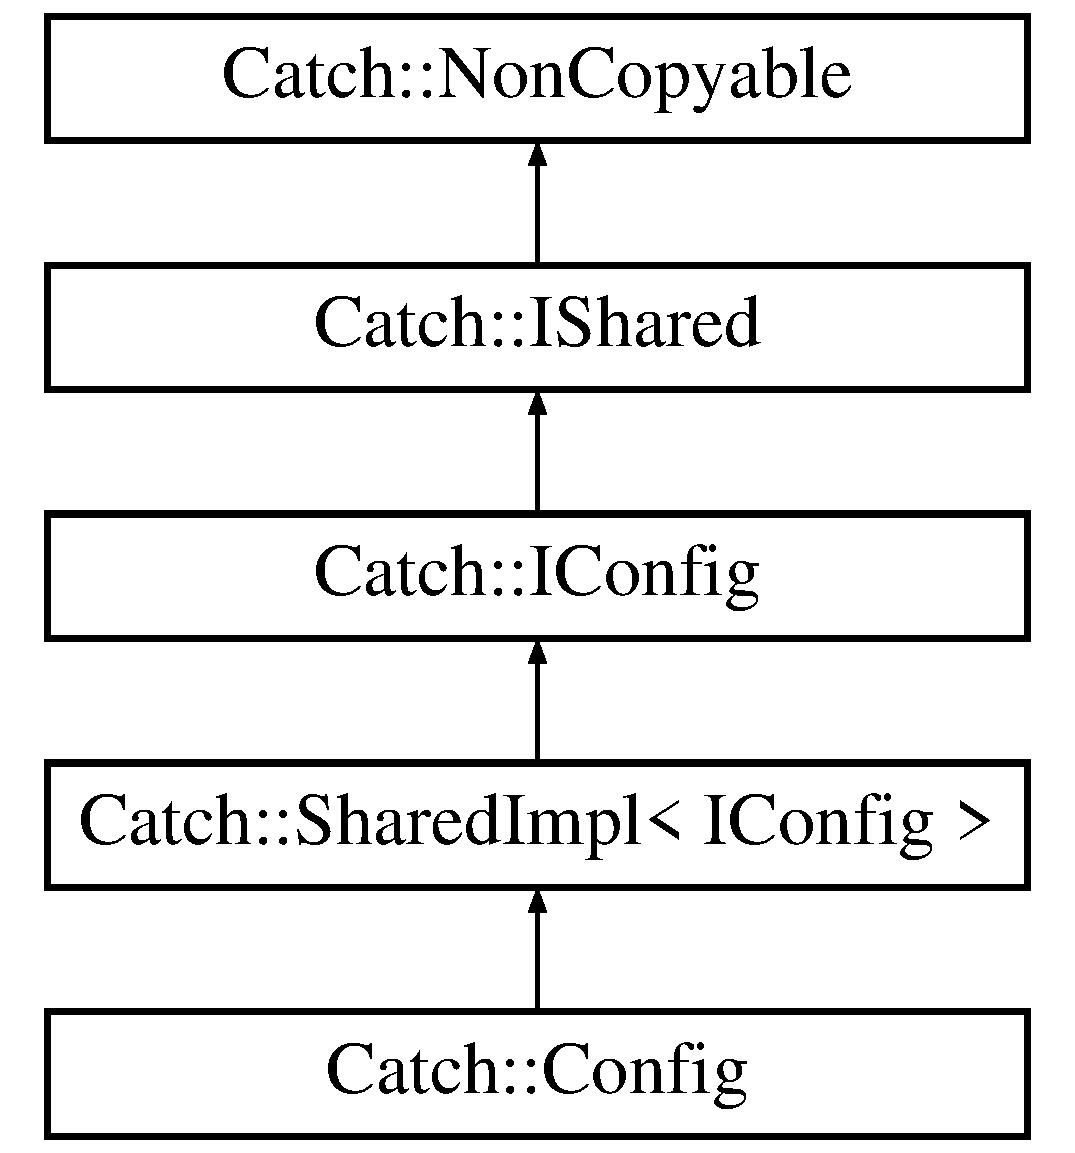
\includegraphics[height=5.000000cm]{struct_catch_1_1_i_config}
\end{center}
\end{figure}
\subsection*{Public Member Functions}
\begin{DoxyCompactItemize}
\item 
\hypertarget{struct_catch_1_1_i_config_aadb95f849359de1e6eb915aab063e542}{virtual bool {\bfseries allow\-Throws} () const =0}\label{struct_catch_1_1_i_config_aadb95f849359de1e6eb915aab063e542}

\item 
\hypertarget{struct_catch_1_1_i_config_aa4c3fe0825e7e6ebdcfa6abc7abf3617}{virtual std\-::ostream \& {\bfseries stream} () const =0}\label{struct_catch_1_1_i_config_aa4c3fe0825e7e6ebdcfa6abc7abf3617}

\item 
\hypertarget{struct_catch_1_1_i_config_aa2315800a05c19db71518b1edc39d43b}{virtual std\-::string {\bfseries name} () const =0}\label{struct_catch_1_1_i_config_aa2315800a05c19db71518b1edc39d43b}

\item 
\hypertarget{struct_catch_1_1_i_config_a2f1b0391019b9ce69921527a684eab23}{virtual bool {\bfseries include\-Successful\-Results} () const =0}\label{struct_catch_1_1_i_config_a2f1b0391019b9ce69921527a684eab23}

\item 
\hypertarget{struct_catch_1_1_i_config_a5b886c5aad9001e90f63a7cf0726af63}{virtual bool {\bfseries should\-Debug\-Break} () const =0}\label{struct_catch_1_1_i_config_a5b886c5aad9001e90f63a7cf0726af63}

\item 
\hypertarget{struct_catch_1_1_i_config_a75d970c495a28e46b8e9b04a1d32149f}{virtual bool {\bfseries warn\-About\-Missing\-Assertions} () const =0}\label{struct_catch_1_1_i_config_a75d970c495a28e46b8e9b04a1d32149f}

\item 
\hypertarget{struct_catch_1_1_i_config_a363f3388a439d02217f37198eff96744}{virtual int {\bfseries abort\-After} () const =0}\label{struct_catch_1_1_i_config_a363f3388a439d02217f37198eff96744}

\item 
\hypertarget{struct_catch_1_1_i_config_abaa97d281484278291f0d3db6d404aeb}{virtual Show\-Durations\-::\-Or\-Not {\bfseries show\-Durations} () const =0}\label{struct_catch_1_1_i_config_abaa97d281484278291f0d3db6d404aeb}

\end{DoxyCompactItemize}


The documentation for this struct was generated from the following file\-:\begin{DoxyCompactItemize}
\item 
Catch.\-h\end{DoxyCompactItemize}

\hypertarget{struct_catch_1_1_i_context}{\section{Catch\-:\-:I\-Context Struct Reference}
\label{struct_catch_1_1_i_context}\index{Catch\-::\-I\-Context@{Catch\-::\-I\-Context}}
}
Inheritance diagram for Catch\-:\-:I\-Context\-:\begin{figure}[H]
\begin{center}
\leavevmode
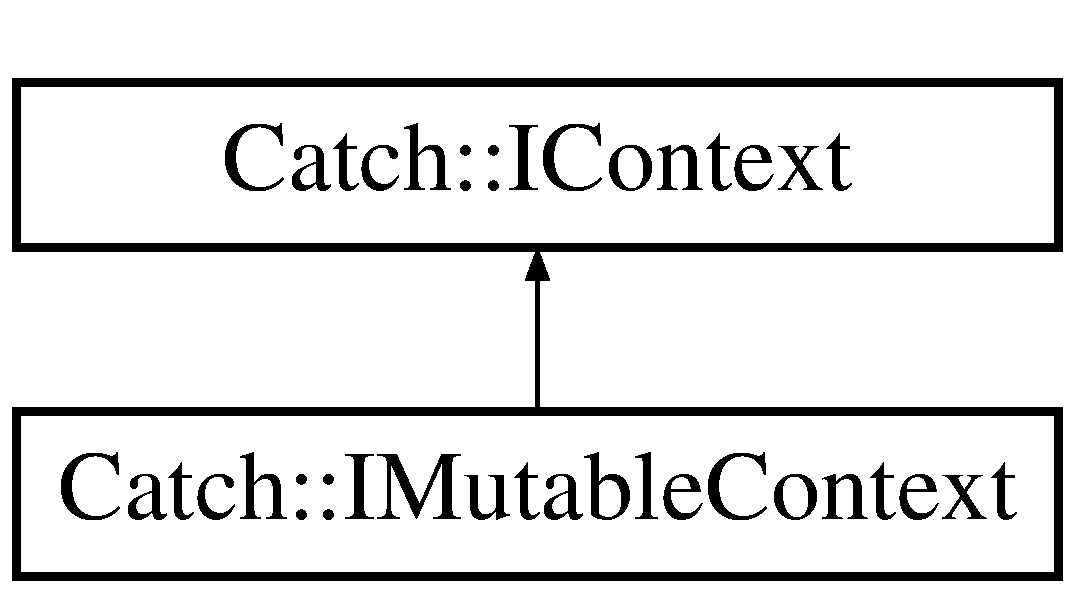
\includegraphics[height=2.000000cm]{struct_catch_1_1_i_context}
\end{center}
\end{figure}
\subsection*{Public Member Functions}
\begin{DoxyCompactItemize}
\item 
\hypertarget{struct_catch_1_1_i_context_a7df92cdf3d2600866bf5aeb56c236cf9}{virtual \hyperlink{struct_catch_1_1_i_result_capture}{I\-Result\-Capture} \& {\bfseries get\-Result\-Capture} ()=0}\label{struct_catch_1_1_i_context_a7df92cdf3d2600866bf5aeb56c236cf9}

\item 
\hypertarget{struct_catch_1_1_i_context_a8106d887b354016f3d79449731b459b9}{virtual \hyperlink{struct_catch_1_1_i_runner}{I\-Runner} \& {\bfseries get\-Runner} ()=0}\label{struct_catch_1_1_i_context_a8106d887b354016f3d79449731b459b9}

\item 
\hypertarget{struct_catch_1_1_i_context_a43e07088db43299ba129fbe6d3106e95}{virtual size\-\_\-t {\bfseries get\-Generator\-Index} (std\-::string const \&file\-Info, size\-\_\-t total\-Size)=0}\label{struct_catch_1_1_i_context_a43e07088db43299ba129fbe6d3106e95}

\item 
\hypertarget{struct_catch_1_1_i_context_a806f7c4ed24d51adae90418e661b24b7}{virtual bool {\bfseries advance\-Generators\-For\-Current\-Test} ()=0}\label{struct_catch_1_1_i_context_a806f7c4ed24d51adae90418e661b24b7}

\item 
\hypertarget{struct_catch_1_1_i_context_aee81c415899262e096ad8d6f686fa365}{virtual \hyperlink{class_catch_1_1_ptr}{Ptr}$<$ \hyperlink{struct_catch_1_1_i_config}{I\-Config} const  $>$ {\bfseries get\-Config} () const =0}\label{struct_catch_1_1_i_context_aee81c415899262e096ad8d6f686fa365}

\end{DoxyCompactItemize}


The documentation for this struct was generated from the following file\-:\begin{DoxyCompactItemize}
\item 
Catch.\-h\end{DoxyCompactItemize}

\hypertarget{struct_catch_1_1_i_exception_translator}{\section{Catch\-:\-:I\-Exception\-Translator Struct Reference}
\label{struct_catch_1_1_i_exception_translator}\index{Catch\-::\-I\-Exception\-Translator@{Catch\-::\-I\-Exception\-Translator}}
}


Inherited by Catch\-::\-Exception\-Translator\-Registrar\-::\-Exception\-Translator$<$ T $>$.

\subsection*{Public Member Functions}
\begin{DoxyCompactItemize}
\item 
\hypertarget{struct_catch_1_1_i_exception_translator_ade89aa305d8c89576521e76b2d1f82eb}{virtual std\-::string {\bfseries translate} () const =0}\label{struct_catch_1_1_i_exception_translator_ade89aa305d8c89576521e76b2d1f82eb}

\end{DoxyCompactItemize}


The documentation for this struct was generated from the following file\-:\begin{DoxyCompactItemize}
\item 
Catch.\-h\end{DoxyCompactItemize}

\hypertarget{struct_catch_1_1_i_exception_translator_registry}{\section{Catch\-:\-:I\-Exception\-Translator\-Registry Struct Reference}
\label{struct_catch_1_1_i_exception_translator_registry}\index{Catch\-::\-I\-Exception\-Translator\-Registry@{Catch\-::\-I\-Exception\-Translator\-Registry}}
}
\subsection*{Public Member Functions}
\begin{DoxyCompactItemize}
\item 
\hypertarget{struct_catch_1_1_i_exception_translator_registry_af76ae8c331a17f2a94c9720bc0d686bb}{virtual std\-::string {\bfseries translate\-Active\-Exception} () const =0}\label{struct_catch_1_1_i_exception_translator_registry_af76ae8c331a17f2a94c9720bc0d686bb}

\end{DoxyCompactItemize}


The documentation for this struct was generated from the following file\-:\begin{DoxyCompactItemize}
\item 
Catch.\-h\end{DoxyCompactItemize}

\hypertarget{struct_catch_1_1_if_filter_matches}{\section{Catch\-:\-:If\-Filter\-Matches Struct Reference}
\label{struct_catch_1_1_if_filter_matches}\index{Catch\-::\-If\-Filter\-Matches@{Catch\-::\-If\-Filter\-Matches}}
}
\subsection*{Public Types}
\begin{DoxyCompactItemize}
\item 
enum {\bfseries Do\-What} \{ {\bfseries Auto\-Detect\-Behaviour}, 
{\bfseries Include\-Tests}, 
{\bfseries Exclude\-Tests}
 \}
\end{DoxyCompactItemize}


The documentation for this struct was generated from the following file\-:\begin{DoxyCompactItemize}
\item 
Catch.\-h\end{DoxyCompactItemize}

\hypertarget{struct_catch_1_1_i_generator}{\section{Catch\-:\-:I\-Generator$<$ T $>$ Struct Template Reference}
\label{struct_catch_1_1_i_generator}\index{Catch\-::\-I\-Generator$<$ T $>$@{Catch\-::\-I\-Generator$<$ T $>$}}
}
Inheritance diagram for Catch\-:\-:I\-Generator$<$ T $>$\-:\begin{figure}[H]
\begin{center}
\leavevmode
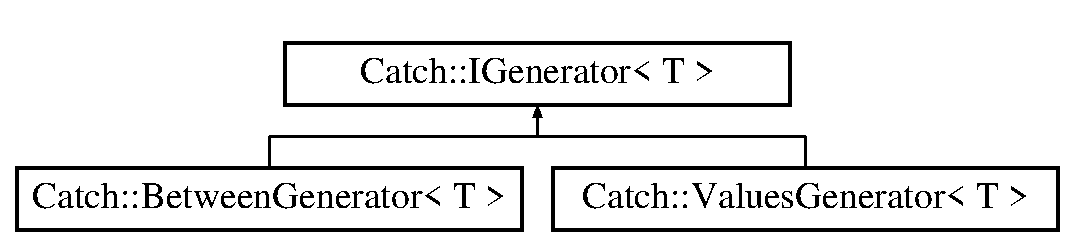
\includegraphics[height=2.000000cm]{struct_catch_1_1_i_generator}
\end{center}
\end{figure}
\subsection*{Public Member Functions}
\begin{DoxyCompactItemize}
\item 
\hypertarget{struct_catch_1_1_i_generator_ad69e937cb66dba3ed9429c42abf4fce3}{virtual T {\bfseries get\-Value} (std\-::size\-\_\-t index) const =0}\label{struct_catch_1_1_i_generator_ad69e937cb66dba3ed9429c42abf4fce3}

\item 
\hypertarget{struct_catch_1_1_i_generator_a2e317253b03e838b6065ce69719a198e}{virtual std\-::size\-\_\-t {\bfseries size} () const =0}\label{struct_catch_1_1_i_generator_a2e317253b03e838b6065ce69719a198e}

\end{DoxyCompactItemize}


The documentation for this struct was generated from the following file\-:\begin{DoxyCompactItemize}
\item 
Catch.\-h\end{DoxyCompactItemize}

\hypertarget{struct_catch_1_1_i_generator_info}{\section{Catch\-:\-:I\-Generator\-Info Struct Reference}
\label{struct_catch_1_1_i_generator_info}\index{Catch\-::\-I\-Generator\-Info@{Catch\-::\-I\-Generator\-Info}}
}
\subsection*{Public Member Functions}
\begin{DoxyCompactItemize}
\item 
\hypertarget{struct_catch_1_1_i_generator_info_a2b86711ca7009903edfe27ed62b515ef}{virtual bool {\bfseries move\-Next} ()=0}\label{struct_catch_1_1_i_generator_info_a2b86711ca7009903edfe27ed62b515ef}

\item 
\hypertarget{struct_catch_1_1_i_generator_info_a6a0dca712d31f6849fd9447b1344673a}{virtual std\-::size\-\_\-t {\bfseries get\-Current\-Index} () const =0}\label{struct_catch_1_1_i_generator_info_a6a0dca712d31f6849fd9447b1344673a}

\end{DoxyCompactItemize}


The documentation for this struct was generated from the following file\-:\begin{DoxyCompactItemize}
\item 
Catch.\-h\end{DoxyCompactItemize}

\hypertarget{struct_catch_1_1_i_generators_for_test}{\section{Catch\-:\-:I\-Generators\-For\-Test Struct Reference}
\label{struct_catch_1_1_i_generators_for_test}\index{Catch\-::\-I\-Generators\-For\-Test@{Catch\-::\-I\-Generators\-For\-Test}}
}
\subsection*{Public Member Functions}
\begin{DoxyCompactItemize}
\item 
\hypertarget{struct_catch_1_1_i_generators_for_test_a180d84e858840188e4c3788e47eefdb0}{virtual \hyperlink{struct_catch_1_1_i_generator_info}{I\-Generator\-Info} \& {\bfseries get\-Generator\-Info} (std\-::string const \&file\-Info, std\-::size\-\_\-t size)=0}\label{struct_catch_1_1_i_generators_for_test_a180d84e858840188e4c3788e47eefdb0}

\item 
\hypertarget{struct_catch_1_1_i_generators_for_test_adab31832d529fc584fd63164e0a1c8ad}{virtual bool {\bfseries move\-Next} ()=0}\label{struct_catch_1_1_i_generators_for_test_adab31832d529fc584fd63164e0a1c8ad}

\end{DoxyCompactItemize}


The documentation for this struct was generated from the following file\-:\begin{DoxyCompactItemize}
\item 
Catch.\-h\end{DoxyCompactItemize}

\hypertarget{struct_catch_1_1_i_mutable_context}{\section{Catch\-:\-:I\-Mutable\-Context Struct Reference}
\label{struct_catch_1_1_i_mutable_context}\index{Catch\-::\-I\-Mutable\-Context@{Catch\-::\-I\-Mutable\-Context}}
}
Inheritance diagram for Catch\-:\-:I\-Mutable\-Context\-:\begin{figure}[H]
\begin{center}
\leavevmode
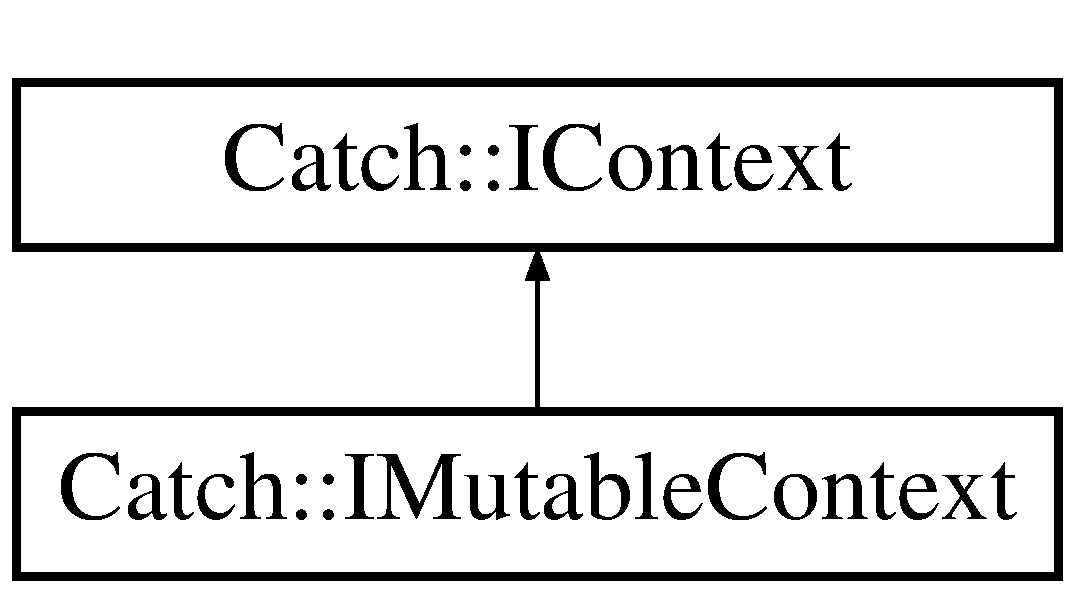
\includegraphics[height=2.000000cm]{struct_catch_1_1_i_mutable_context}
\end{center}
\end{figure}
\subsection*{Public Member Functions}
\begin{DoxyCompactItemize}
\item 
\hypertarget{struct_catch_1_1_i_mutable_context_a4a80afd0525b7def21bee8d9b48f2d39}{virtual void {\bfseries set\-Result\-Capture} (\hyperlink{struct_catch_1_1_i_result_capture}{I\-Result\-Capture} $\ast$result\-Capture)=0}\label{struct_catch_1_1_i_mutable_context_a4a80afd0525b7def21bee8d9b48f2d39}

\item 
\hypertarget{struct_catch_1_1_i_mutable_context_af2e53b1dea4527a2587cff266a730f6e}{virtual void {\bfseries set\-Runner} (\hyperlink{struct_catch_1_1_i_runner}{I\-Runner} $\ast$runner)=0}\label{struct_catch_1_1_i_mutable_context_af2e53b1dea4527a2587cff266a730f6e}

\item 
\hypertarget{struct_catch_1_1_i_mutable_context_a04ae4f4219a481a7bf658d9fd445bc1d}{virtual void {\bfseries set\-Config} (\hyperlink{class_catch_1_1_ptr}{Ptr}$<$ \hyperlink{struct_catch_1_1_i_config}{I\-Config} const  $>$ const \&config)=0}\label{struct_catch_1_1_i_mutable_context_a04ae4f4219a481a7bf658d9fd445bc1d}

\end{DoxyCompactItemize}


The documentation for this struct was generated from the following file\-:\begin{DoxyCompactItemize}
\item 
Catch.\-h\end{DoxyCompactItemize}

\hypertarget{struct_catch_1_1_i_mutable_registry_hub}{\section{Catch\-:\-:I\-Mutable\-Registry\-Hub Struct Reference}
\label{struct_catch_1_1_i_mutable_registry_hub}\index{Catch\-::\-I\-Mutable\-Registry\-Hub@{Catch\-::\-I\-Mutable\-Registry\-Hub}}
}
\subsection*{Public Member Functions}
\begin{DoxyCompactItemize}
\item 
\hypertarget{struct_catch_1_1_i_mutable_registry_hub_a1f61ed2b3f2d160b31a0f2c1d9a52af1}{virtual void {\bfseries register\-Reporter} (std\-::string const \&name, \hyperlink{struct_catch_1_1_i_reporter_factory}{I\-Reporter\-Factory} $\ast$factory)=0}\label{struct_catch_1_1_i_mutable_registry_hub_a1f61ed2b3f2d160b31a0f2c1d9a52af1}

\item 
\hypertarget{struct_catch_1_1_i_mutable_registry_hub_a11b85c6744d88c9f83fe16ad4a8dd451}{virtual void {\bfseries register\-Test} (\hyperlink{class_catch_1_1_test_case}{Test\-Case} const \&test\-Info)=0}\label{struct_catch_1_1_i_mutable_registry_hub_a11b85c6744d88c9f83fe16ad4a8dd451}

\item 
\hypertarget{struct_catch_1_1_i_mutable_registry_hub_ae6825365102693cf7707db022a2c2b49}{virtual void {\bfseries register\-Translator} (const \hyperlink{struct_catch_1_1_i_exception_translator}{I\-Exception\-Translator} $\ast$translator)=0}\label{struct_catch_1_1_i_mutable_registry_hub_ae6825365102693cf7707db022a2c2b49}

\end{DoxyCompactItemize}


The documentation for this struct was generated from the following file\-:\begin{DoxyCompactItemize}
\item 
Catch.\-h\end{DoxyCompactItemize}

\hypertarget{struct_catch_1_1_i_registry_hub}{\section{Catch\-:\-:I\-Registry\-Hub Struct Reference}
\label{struct_catch_1_1_i_registry_hub}\index{Catch\-::\-I\-Registry\-Hub@{Catch\-::\-I\-Registry\-Hub}}
}
\subsection*{Public Member Functions}
\begin{DoxyCompactItemize}
\item 
\hypertarget{struct_catch_1_1_i_registry_hub_a55534563f7ecf7e20ec1e37285ebe54d}{virtual \hyperlink{struct_catch_1_1_i_reporter_registry}{I\-Reporter\-Registry} const \& {\bfseries get\-Reporter\-Registry} () const =0}\label{struct_catch_1_1_i_registry_hub_a55534563f7ecf7e20ec1e37285ebe54d}

\item 
\hypertarget{struct_catch_1_1_i_registry_hub_af4f6255f0c0f8f1f179fa9d7d4843076}{virtual \hyperlink{struct_catch_1_1_i_test_case_registry}{I\-Test\-Case\-Registry} const \& {\bfseries get\-Test\-Case\-Registry} () const =0}\label{struct_catch_1_1_i_registry_hub_af4f6255f0c0f8f1f179fa9d7d4843076}

\item 
\hypertarget{struct_catch_1_1_i_registry_hub_a3606988da110c016c5af3ae63454eb78}{virtual \\*
\hyperlink{struct_catch_1_1_i_exception_translator_registry}{I\-Exception\-Translator\-Registry} \& {\bfseries get\-Exception\-Translator\-Registry} ()=0}\label{struct_catch_1_1_i_registry_hub_a3606988da110c016c5af3ae63454eb78}

\end{DoxyCompactItemize}


The documentation for this struct was generated from the following file\-:\begin{DoxyCompactItemize}
\item 
Catch.\-h\end{DoxyCompactItemize}

\hypertarget{struct_catch_1_1_i_reporter}{\section{Catch\-:\-:I\-Reporter Struct Reference}
\label{struct_catch_1_1_i_reporter}\index{Catch\-::\-I\-Reporter@{Catch\-::\-I\-Reporter}}
}
Inheritance diagram for Catch\-:\-:I\-Reporter\-:\begin{figure}[H]
\begin{center}
\leavevmode
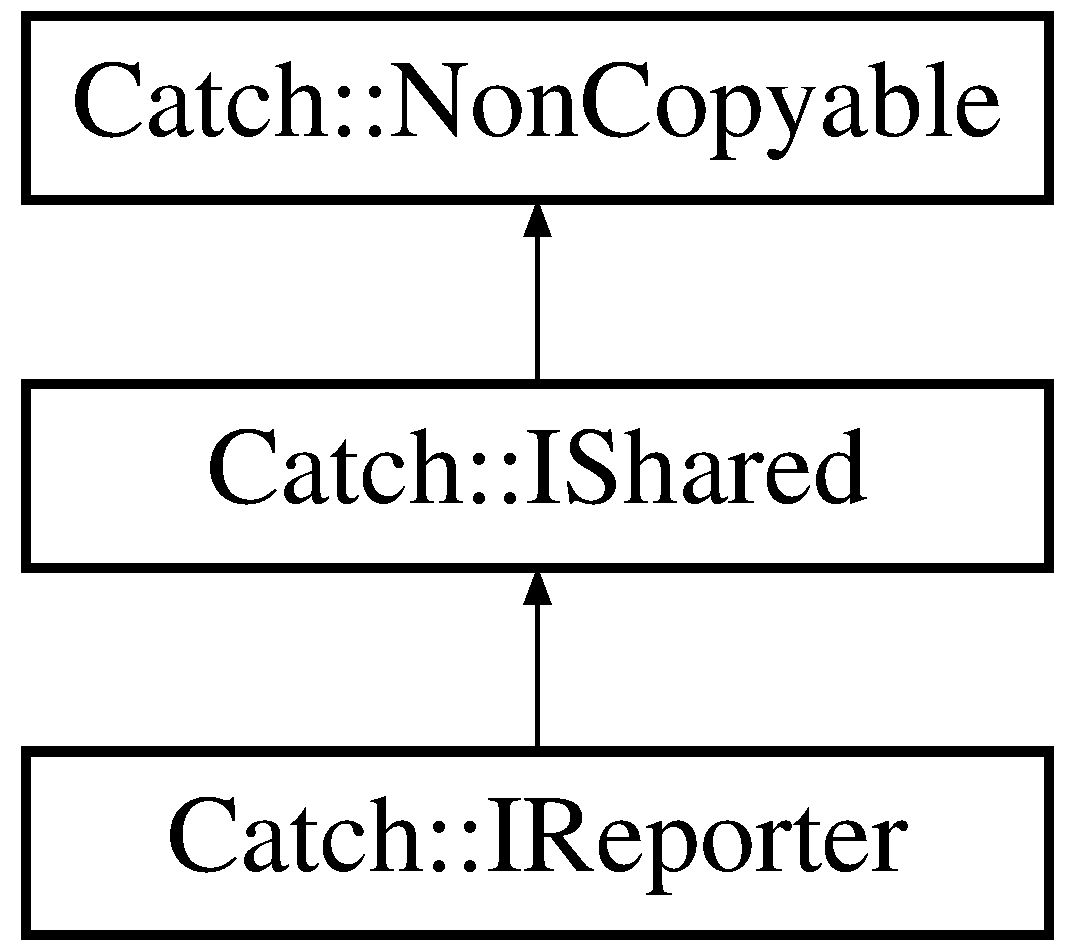
\includegraphics[height=3.000000cm]{struct_catch_1_1_i_reporter}
\end{center}
\end{figure}
\subsection*{Public Member Functions}
\begin{DoxyCompactItemize}
\item 
\hypertarget{struct_catch_1_1_i_reporter_aebd8c20478de29bba9b5a9f3845c18dc}{virtual bool {\bfseries should\-Redirect\-Stdout} () const =0}\label{struct_catch_1_1_i_reporter_aebd8c20478de29bba9b5a9f3845c18dc}

\item 
\hypertarget{struct_catch_1_1_i_reporter_afcf38d6ff912a9b2c7f07da45fcd5cb1}{virtual void {\bfseries Start\-Testing} ()=0}\label{struct_catch_1_1_i_reporter_afcf38d6ff912a9b2c7f07da45fcd5cb1}

\item 
\hypertarget{struct_catch_1_1_i_reporter_a8f1ae9b07d7feb22f6b1ca61924a6cbf}{virtual void {\bfseries End\-Testing} (\hyperlink{struct_catch_1_1_totals}{Totals} const \&totals)=0}\label{struct_catch_1_1_i_reporter_a8f1ae9b07d7feb22f6b1ca61924a6cbf}

\item 
\hypertarget{struct_catch_1_1_i_reporter_a8bbe6459db57886e80ee312aa38af8e0}{virtual void {\bfseries Start\-Group} (std\-::string const \&group\-Name)=0}\label{struct_catch_1_1_i_reporter_a8bbe6459db57886e80ee312aa38af8e0}

\item 
\hypertarget{struct_catch_1_1_i_reporter_a8b19ae2efce9057bf47e10720c5a4c16}{virtual void {\bfseries End\-Group} (std\-::string const \&group\-Name, \hyperlink{struct_catch_1_1_totals}{Totals} const \&totals)=0}\label{struct_catch_1_1_i_reporter_a8b19ae2efce9057bf47e10720c5a4c16}

\item 
\hypertarget{struct_catch_1_1_i_reporter_aeedd3dd4036feec8bd8866383fddacaa}{virtual void {\bfseries Start\-Test\-Case} (\hyperlink{struct_catch_1_1_test_case_info}{Test\-Case\-Info} const \&test\-Info)=0}\label{struct_catch_1_1_i_reporter_aeedd3dd4036feec8bd8866383fddacaa}

\item 
\hypertarget{struct_catch_1_1_i_reporter_a3da1e768e205533165e2fda4af7e0f4f}{virtual void {\bfseries End\-Test\-Case} (\hyperlink{struct_catch_1_1_test_case_info}{Test\-Case\-Info} const \&test\-Info, \hyperlink{struct_catch_1_1_totals}{Totals} const \&totals, std\-::string const \&std\-Out, std\-::string const \&std\-Err)=0}\label{struct_catch_1_1_i_reporter_a3da1e768e205533165e2fda4af7e0f4f}

\item 
\hypertarget{struct_catch_1_1_i_reporter_a8fc7f21b3d03083f1633431f47534404}{virtual void {\bfseries Start\-Section} (std\-::string const \&section\-Name, std\-::string const \&description)=0}\label{struct_catch_1_1_i_reporter_a8fc7f21b3d03083f1633431f47534404}

\item 
\hypertarget{struct_catch_1_1_i_reporter_a1bc1fd4b6cd5431a3a8c943c9c4d8d57}{virtual void {\bfseries End\-Section} (std\-::string const \&section\-Name, \hyperlink{struct_catch_1_1_counts}{Counts} const \&assertions)=0}\label{struct_catch_1_1_i_reporter_a1bc1fd4b6cd5431a3a8c943c9c4d8d57}

\item 
\hypertarget{struct_catch_1_1_i_reporter_ad382266a8a98628e5c199c6961734a9e}{virtual void {\bfseries No\-Assertions\-In\-Section} (std\-::string const \&section\-Name)=0}\label{struct_catch_1_1_i_reporter_ad382266a8a98628e5c199c6961734a9e}

\item 
\hypertarget{struct_catch_1_1_i_reporter_afe624f1c1c221703d1bdbf12d2cc058f}{virtual void {\bfseries No\-Assertions\-In\-Test\-Case} (std\-::string const \&test\-Name)=0}\label{struct_catch_1_1_i_reporter_afe624f1c1c221703d1bdbf12d2cc058f}

\item 
\hypertarget{struct_catch_1_1_i_reporter_a00d9d8bedcf32e5fdeed12b620b7ff7e}{virtual void {\bfseries Aborted} ()=0}\label{struct_catch_1_1_i_reporter_a00d9d8bedcf32e5fdeed12b620b7ff7e}

\item 
\hypertarget{struct_catch_1_1_i_reporter_aff9de693fee3a041d022894453140c5a}{virtual void {\bfseries Result} (\hyperlink{class_catch_1_1_assertion_result}{Assertion\-Result} const \&result)=0}\label{struct_catch_1_1_i_reporter_aff9de693fee3a041d022894453140c5a}

\end{DoxyCompactItemize}


The documentation for this struct was generated from the following file\-:\begin{DoxyCompactItemize}
\item 
Catch.\-h\end{DoxyCompactItemize}

\hypertarget{struct_catch_1_1_i_reporter_factory}{\section{Catch\-:\-:I\-Reporter\-Factory Struct Reference}
\label{struct_catch_1_1_i_reporter_factory}\index{Catch\-::\-I\-Reporter\-Factory@{Catch\-::\-I\-Reporter\-Factory}}
}
\subsection*{Public Member Functions}
\begin{DoxyCompactItemize}
\item 
\hypertarget{struct_catch_1_1_i_reporter_factory_aa3c32d75432326148bf585212233a0bf}{virtual \hyperlink{struct_catch_1_1_i_streaming_reporter}{I\-Streaming\-Reporter} $\ast$ {\bfseries create} (\hyperlink{struct_catch_1_1_reporter_config}{Reporter\-Config} const \&config) const =0}\label{struct_catch_1_1_i_reporter_factory_aa3c32d75432326148bf585212233a0bf}

\item 
\hypertarget{struct_catch_1_1_i_reporter_factory_a46880f93bd351d113d8189421928531b}{virtual std\-::string {\bfseries get\-Description} () const =0}\label{struct_catch_1_1_i_reporter_factory_a46880f93bd351d113d8189421928531b}

\end{DoxyCompactItemize}


The documentation for this struct was generated from the following file\-:\begin{DoxyCompactItemize}
\item 
Catch.\-h\end{DoxyCompactItemize}

\hypertarget{struct_catch_1_1_i_reporter_registry}{\section{Catch\-:\-:I\-Reporter\-Registry Struct Reference}
\label{struct_catch_1_1_i_reporter_registry}\index{Catch\-::\-I\-Reporter\-Registry@{Catch\-::\-I\-Reporter\-Registry}}
}
\subsection*{Public Types}
\begin{DoxyCompactItemize}
\item 
\hypertarget{struct_catch_1_1_i_reporter_registry_a328440adc2303a1e31bdc763f0504452}{typedef std\-::map$<$ std\-::string, \\*
\hyperlink{struct_catch_1_1_i_reporter_factory}{I\-Reporter\-Factory} $\ast$ $>$ {\bfseries Factory\-Map}}\label{struct_catch_1_1_i_reporter_registry_a328440adc2303a1e31bdc763f0504452}

\end{DoxyCompactItemize}
\subsection*{Public Member Functions}
\begin{DoxyCompactItemize}
\item 
\hypertarget{struct_catch_1_1_i_reporter_registry_aa755ff8c6f1d29aaf43e0127c70e85d0}{virtual \hyperlink{struct_catch_1_1_i_streaming_reporter}{I\-Streaming\-Reporter} $\ast$ {\bfseries create} (std\-::string const \&name, \hyperlink{class_catch_1_1_ptr}{Ptr}$<$ \hyperlink{struct_catch_1_1_i_config}{I\-Config} $>$ const \&config) const =0}\label{struct_catch_1_1_i_reporter_registry_aa755ff8c6f1d29aaf43e0127c70e85d0}

\item 
\hypertarget{struct_catch_1_1_i_reporter_registry_a76ffc8a26c38929f370196937ed112b5}{virtual Factory\-Map const \& {\bfseries get\-Factories} () const =0}\label{struct_catch_1_1_i_reporter_registry_a76ffc8a26c38929f370196937ed112b5}

\end{DoxyCompactItemize}


The documentation for this struct was generated from the following file\-:\begin{DoxyCompactItemize}
\item 
Catch.\-h\end{DoxyCompactItemize}

\hypertarget{struct_catch_1_1_i_result_capture}{\section{Catch\-:\-:I\-Result\-Capture Struct Reference}
\label{struct_catch_1_1_i_result_capture}\index{Catch\-::\-I\-Result\-Capture@{Catch\-::\-I\-Result\-Capture}}
}
\subsection*{Public Member Functions}
\begin{DoxyCompactItemize}
\item 
\hypertarget{struct_catch_1_1_i_result_capture_ae45e08bccc5fb434656d4f2e44742223}{virtual void {\bfseries assertion\-Ended} (\hyperlink{class_catch_1_1_assertion_result}{Assertion\-Result} const \&result)=0}\label{struct_catch_1_1_i_result_capture_ae45e08bccc5fb434656d4f2e44742223}

\item 
\hypertarget{struct_catch_1_1_i_result_capture_a5b76ed52badcb64cf374202e12b81a03}{virtual bool {\bfseries section\-Started} (\hyperlink{struct_catch_1_1_section_info}{Section\-Info} const \&section\-Info, \hyperlink{struct_catch_1_1_counts}{Counts} \&assertions)=0}\label{struct_catch_1_1_i_result_capture_a5b76ed52badcb64cf374202e12b81a03}

\item 
\hypertarget{struct_catch_1_1_i_result_capture_a110d3d300709d114b3e4718fff021b29}{virtual void {\bfseries section\-Ended} (\hyperlink{struct_catch_1_1_section_info}{Section\-Info} const \&name, \hyperlink{struct_catch_1_1_counts}{Counts} const \&assertions, double \-\_\-duration\-In\-Seconds)=0}\label{struct_catch_1_1_i_result_capture_a110d3d300709d114b3e4718fff021b29}

\item 
\hypertarget{struct_catch_1_1_i_result_capture_a91d154c1e087e383dcde5aad95cb6a05}{virtual void {\bfseries push\-Scoped\-Message} (\hyperlink{struct_catch_1_1_message_info}{Message\-Info} const \&message)=0}\label{struct_catch_1_1_i_result_capture_a91d154c1e087e383dcde5aad95cb6a05}

\item 
\hypertarget{struct_catch_1_1_i_result_capture_a42bcb13276706bf8c3ce081ce16d37fd}{virtual void {\bfseries pop\-Scoped\-Message} (\hyperlink{struct_catch_1_1_message_info}{Message\-Info} const \&message)=0}\label{struct_catch_1_1_i_result_capture_a42bcb13276706bf8c3ce081ce16d37fd}

\item 
\hypertarget{struct_catch_1_1_i_result_capture_a7839e422ccd55f298cd64f0bf4a5938b}{virtual bool {\bfseries should\-Debug\-Break} () const =0}\label{struct_catch_1_1_i_result_capture_a7839e422ccd55f298cd64f0bf4a5938b}

\item 
\hypertarget{struct_catch_1_1_i_result_capture_a76e0229ceb19405d2dd4a868ce0a1cdf}{virtual Result\-Action\-::\-Value {\bfseries accept\-Expression} (\hyperlink{class_catch_1_1_expression_result_builder}{Expression\-Result\-Builder} const \&assertion\-Result, \hyperlink{struct_catch_1_1_assertion_info}{Assertion\-Info} const \&assertion\-Info)=0}\label{struct_catch_1_1_i_result_capture_a76e0229ceb19405d2dd4a868ce0a1cdf}

\item 
\hypertarget{struct_catch_1_1_i_result_capture_aea1617f4a84cc648246aa3ed6918b5bf}{virtual std\-::string {\bfseries get\-Current\-Test\-Name} () const =0}\label{struct_catch_1_1_i_result_capture_aea1617f4a84cc648246aa3ed6918b5bf}

\item 
\hypertarget{struct_catch_1_1_i_result_capture_ab18872c89fab97405a56e9c6a4919736}{virtual const \hyperlink{class_catch_1_1_assertion_result}{Assertion\-Result} $\ast$ {\bfseries get\-Last\-Result} () const =0}\label{struct_catch_1_1_i_result_capture_ab18872c89fab97405a56e9c6a4919736}

\end{DoxyCompactItemize}


The documentation for this struct was generated from the following file\-:\begin{DoxyCompactItemize}
\item 
Catch.\-h\end{DoxyCompactItemize}

\hypertarget{struct_catch_1_1_i_runner}{\section{Catch\-:\-:I\-Runner Struct Reference}
\label{struct_catch_1_1_i_runner}\index{Catch\-::\-I\-Runner@{Catch\-::\-I\-Runner}}
}


The documentation for this struct was generated from the following file\-:\begin{DoxyCompactItemize}
\item 
Catch.\-h\end{DoxyCompactItemize}

\hypertarget{struct_catch_1_1_i_shared}{\section{Catch\-:\-:I\-Shared Struct Reference}
\label{struct_catch_1_1_i_shared}\index{Catch\-::\-I\-Shared@{Catch\-::\-I\-Shared}}
}
Inheritance diagram for Catch\-:\-:I\-Shared\-:\begin{figure}[H]
\begin{center}
\leavevmode
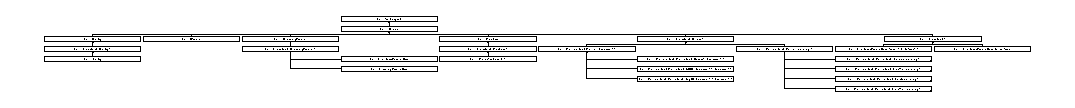
\includegraphics[height=1.002237cm]{struct_catch_1_1_i_shared}
\end{center}
\end{figure}
\subsection*{Public Member Functions}
\begin{DoxyCompactItemize}
\item 
\hypertarget{struct_catch_1_1_i_shared_ae383df68557cdaf0910b411af04d9e33}{virtual void {\bfseries add\-Ref} () const =0}\label{struct_catch_1_1_i_shared_ae383df68557cdaf0910b411af04d9e33}

\item 
\hypertarget{struct_catch_1_1_i_shared_a002f52624728a763956fb6f230cb2f57}{virtual void {\bfseries release} () const =0}\label{struct_catch_1_1_i_shared_a002f52624728a763956fb6f230cb2f57}

\end{DoxyCompactItemize}


The documentation for this struct was generated from the following file\-:\begin{DoxyCompactItemize}
\item 
Catch.\-h\end{DoxyCompactItemize}

\hypertarget{struct_catch_1_1_detail_1_1_is_stream_insertable}{\section{Catch\-:\-:Detail\-:\-:Is\-Stream\-Insertable$<$ T $>$ Struct Template Reference}
\label{struct_catch_1_1_detail_1_1_is_stream_insertable}\index{Catch\-::\-Detail\-::\-Is\-Stream\-Insertable$<$ T $>$@{Catch\-::\-Detail\-::\-Is\-Stream\-Insertable$<$ T $>$}}
}
\subsection*{Public Types}
\begin{DoxyCompactItemize}
\item 
enum \{ {\bfseries value} = sizeof( test\-Streamable(s $<$$<$ t) ) == sizeof( True\-Type )
 \}
\end{DoxyCompactItemize}
\subsection*{Static Public Attributes}
\begin{DoxyCompactItemize}
\item 
\hypertarget{struct_catch_1_1_detail_1_1_is_stream_insertable_abe3d3c8e5d85665747faafffc9a96b00}{static std\-::ostream \& {\bfseries s}}\label{struct_catch_1_1_detail_1_1_is_stream_insertable_abe3d3c8e5d85665747faafffc9a96b00}

\item 
\hypertarget{struct_catch_1_1_detail_1_1_is_stream_insertable_a7d2a3da978b6736667a7b2f6d51f507f}{static T const \& {\bfseries t}}\label{struct_catch_1_1_detail_1_1_is_stream_insertable_a7d2a3da978b6736667a7b2f6d51f507f}

\end{DoxyCompactItemize}


The documentation for this struct was generated from the following file\-:\begin{DoxyCompactItemize}
\item 
Catch.\-h\end{DoxyCompactItemize}

\hypertarget{struct_catch_1_1_i_streaming_reporter}{\section{Catch\-:\-:I\-Streaming\-Reporter Struct Reference}
\label{struct_catch_1_1_i_streaming_reporter}\index{Catch\-::\-I\-Streaming\-Reporter@{Catch\-::\-I\-Streaming\-Reporter}}
}
Inheritance diagram for Catch\-:\-:I\-Streaming\-Reporter\-:\begin{figure}[H]
\begin{center}
\leavevmode
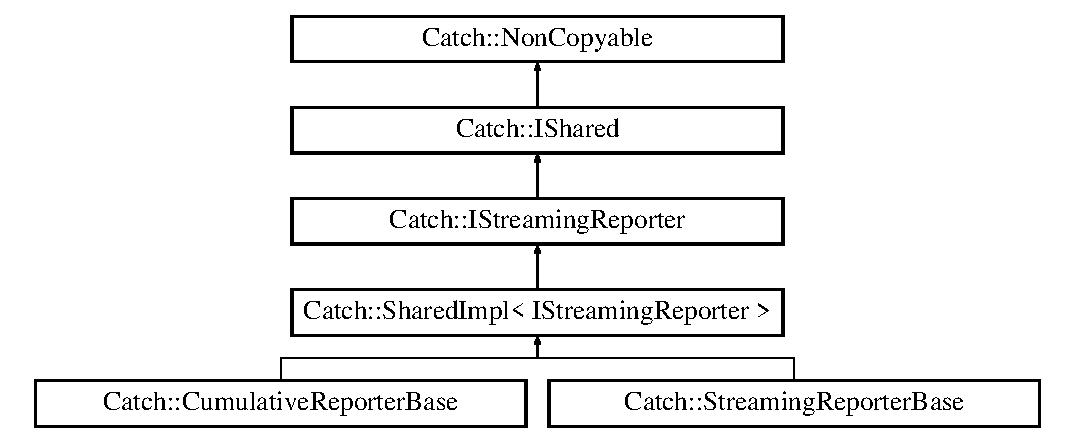
\includegraphics[height=5.000000cm]{struct_catch_1_1_i_streaming_reporter}
\end{center}
\end{figure}
\subsection*{Public Member Functions}
\begin{DoxyCompactItemize}
\item 
\hypertarget{struct_catch_1_1_i_streaming_reporter_a122d9136175aefb16ccc5d3b61f23711}{virtual \hyperlink{struct_catch_1_1_reporter_preferences}{Reporter\-Preferences} {\bfseries get\-Preferences} () const =0}\label{struct_catch_1_1_i_streaming_reporter_a122d9136175aefb16ccc5d3b61f23711}

\item 
\hypertarget{struct_catch_1_1_i_streaming_reporter_aaa0ea1d8250b48fafc8d36f86e6d1d80}{virtual void {\bfseries no\-Matching\-Test\-Cases} (std\-::string const \&spec)=0}\label{struct_catch_1_1_i_streaming_reporter_aaa0ea1d8250b48fafc8d36f86e6d1d80}

\item 
\hypertarget{struct_catch_1_1_i_streaming_reporter_a8c7b304d9563992a611dc7d68dc0c1ce}{virtual void {\bfseries test\-Run\-Starting} (\hyperlink{struct_catch_1_1_test_run_info}{Test\-Run\-Info} const \&test\-Run\-Info)=0}\label{struct_catch_1_1_i_streaming_reporter_a8c7b304d9563992a611dc7d68dc0c1ce}

\item 
\hypertarget{struct_catch_1_1_i_streaming_reporter_aef40d16994fe8a7ab140c885d8c2d7d0}{virtual void {\bfseries test\-Group\-Starting} (\hyperlink{struct_catch_1_1_group_info}{Group\-Info} const \&group\-Info)=0}\label{struct_catch_1_1_i_streaming_reporter_aef40d16994fe8a7ab140c885d8c2d7d0}

\item 
\hypertarget{struct_catch_1_1_i_streaming_reporter_a8f7270dc83853494a1c3a912ddf95a11}{virtual void {\bfseries test\-Case\-Starting} (\hyperlink{struct_catch_1_1_test_case_info}{Test\-Case\-Info} const \&test\-Info)=0}\label{struct_catch_1_1_i_streaming_reporter_a8f7270dc83853494a1c3a912ddf95a11}

\item 
\hypertarget{struct_catch_1_1_i_streaming_reporter_aa6236178937a43c2d7665729fcb79521}{virtual void {\bfseries section\-Starting} (\hyperlink{struct_catch_1_1_section_info}{Section\-Info} const \&section\-Info)=0}\label{struct_catch_1_1_i_streaming_reporter_aa6236178937a43c2d7665729fcb79521}

\item 
\hypertarget{struct_catch_1_1_i_streaming_reporter_ae1c3becff20f4a940c9f01d2c4114a17}{virtual void {\bfseries assertion\-Starting} (\hyperlink{struct_catch_1_1_assertion_info}{Assertion\-Info} const \&assertion\-Info)=0}\label{struct_catch_1_1_i_streaming_reporter_ae1c3becff20f4a940c9f01d2c4114a17}

\item 
\hypertarget{struct_catch_1_1_i_streaming_reporter_a5248ab87149e0f1abe2de96c387ff5e3}{virtual bool {\bfseries assertion\-Ended} (\hyperlink{struct_catch_1_1_assertion_stats}{Assertion\-Stats} const \&assertion\-Stats)=0}\label{struct_catch_1_1_i_streaming_reporter_a5248ab87149e0f1abe2de96c387ff5e3}

\item 
\hypertarget{struct_catch_1_1_i_streaming_reporter_aba7a6ce1f315da47b8017b5ca6d1d008}{virtual void {\bfseries section\-Ended} (\hyperlink{struct_catch_1_1_section_stats}{Section\-Stats} const \&section\-Stats)=0}\label{struct_catch_1_1_i_streaming_reporter_aba7a6ce1f315da47b8017b5ca6d1d008}

\item 
\hypertarget{struct_catch_1_1_i_streaming_reporter_ae295b98b77bab527be53ea9d35dfe66f}{virtual void {\bfseries test\-Case\-Ended} (\hyperlink{struct_catch_1_1_test_case_stats}{Test\-Case\-Stats} const \&test\-Case\-Stats)=0}\label{struct_catch_1_1_i_streaming_reporter_ae295b98b77bab527be53ea9d35dfe66f}

\item 
\hypertarget{struct_catch_1_1_i_streaming_reporter_abf668bf347eda4ba94fa2b3483ca4dd3}{virtual void {\bfseries test\-Group\-Ended} (\hyperlink{struct_catch_1_1_test_group_stats}{Test\-Group\-Stats} const \&test\-Group\-Stats)=0}\label{struct_catch_1_1_i_streaming_reporter_abf668bf347eda4ba94fa2b3483ca4dd3}

\item 
\hypertarget{struct_catch_1_1_i_streaming_reporter_a1ac383df84242bc55578e32ebca13e88}{virtual void {\bfseries test\-Run\-Ended} (\hyperlink{struct_catch_1_1_test_run_stats}{Test\-Run\-Stats} const \&test\-Run\-Stats)=0}\label{struct_catch_1_1_i_streaming_reporter_a1ac383df84242bc55578e32ebca13e88}

\end{DoxyCompactItemize}


The documentation for this struct was generated from the following file\-:\begin{DoxyCompactItemize}
\item 
Catch.\-h\end{DoxyCompactItemize}

\hypertarget{struct_catch_1_1_i_test_case}{\section{Catch\-:\-:I\-Test\-Case Struct Reference}
\label{struct_catch_1_1_i_test_case}\index{Catch\-::\-I\-Test\-Case@{Catch\-::\-I\-Test\-Case}}
}
Inheritance diagram for Catch\-:\-:I\-Test\-Case\-:\begin{figure}[H]
\begin{center}
\leavevmode
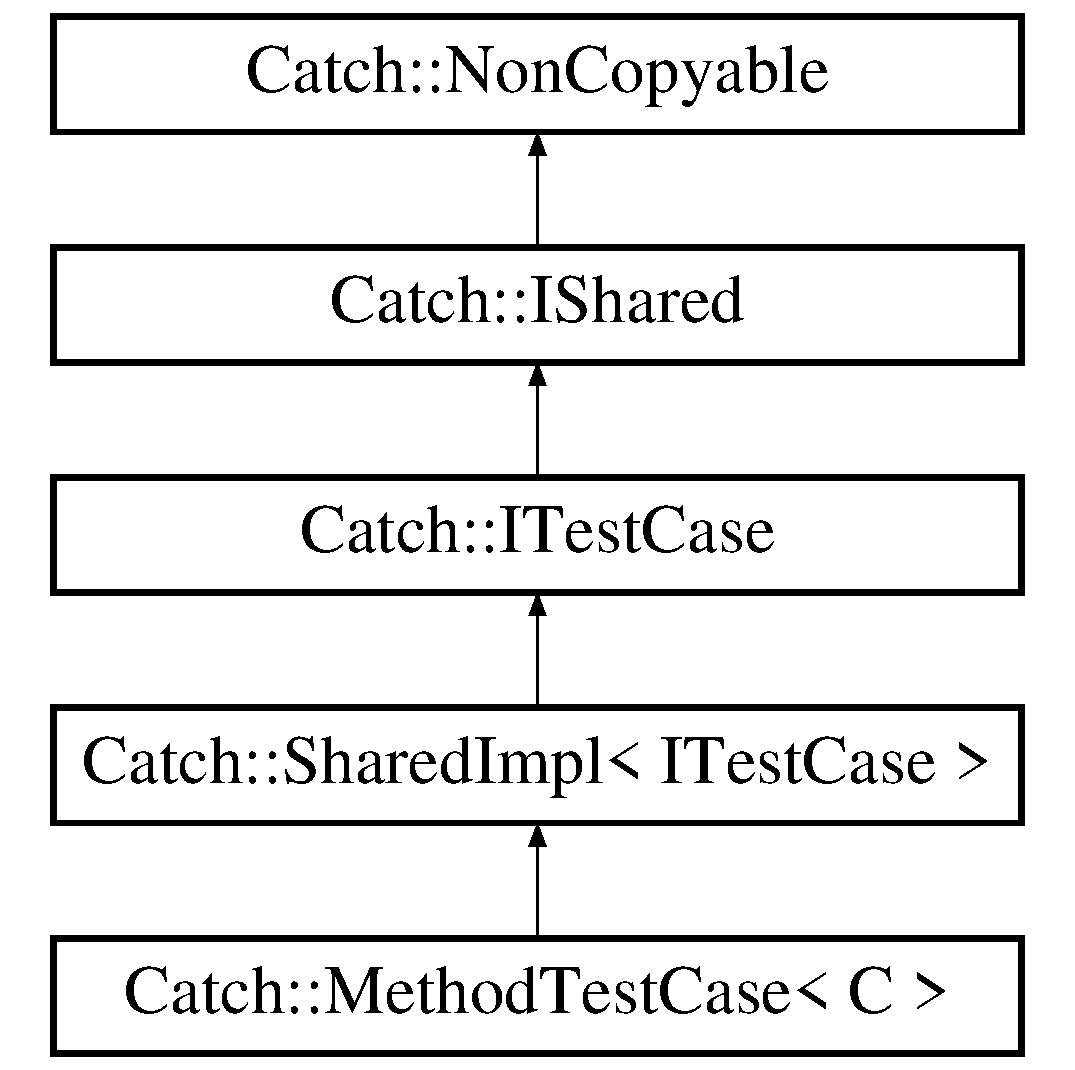
\includegraphics[height=5.000000cm]{struct_catch_1_1_i_test_case}
\end{center}
\end{figure}
\subsection*{Public Member Functions}
\begin{DoxyCompactItemize}
\item 
\hypertarget{struct_catch_1_1_i_test_case_a678825e62e7c17297621cfeb65588c34}{virtual void {\bfseries invoke} () const =0}\label{struct_catch_1_1_i_test_case_a678825e62e7c17297621cfeb65588c34}

\end{DoxyCompactItemize}


The documentation for this struct was generated from the following file\-:\begin{DoxyCompactItemize}
\item 
Catch.\-h\end{DoxyCompactItemize}

\hypertarget{struct_catch_1_1_i_test_case_registry}{\section{Catch\-:\-:I\-Test\-Case\-Registry Struct Reference}
\label{struct_catch_1_1_i_test_case_registry}\index{Catch\-::\-I\-Test\-Case\-Registry@{Catch\-::\-I\-Test\-Case\-Registry}}
}
\subsection*{Public Member Functions}
\begin{DoxyCompactItemize}
\item 
\hypertarget{struct_catch_1_1_i_test_case_registry_ad6e4d4a621655123f73ae98cfeda063d}{virtual std\-::vector$<$ \hyperlink{class_catch_1_1_test_case}{Test\-Case} $>$\\*
 const \& {\bfseries get\-All\-Tests} () const =0}\label{struct_catch_1_1_i_test_case_registry_ad6e4d4a621655123f73ae98cfeda063d}

\item 
\hypertarget{struct_catch_1_1_i_test_case_registry_ac112a15cfde63b4a6aedab22934d0ce5}{virtual std\-::vector$<$ \hyperlink{class_catch_1_1_test_case}{Test\-Case} $>$ {\bfseries get\-Matching\-Test\-Cases} (std\-::string const \&raw\-Test\-Spec) const =0}\label{struct_catch_1_1_i_test_case_registry_ac112a15cfde63b4a6aedab22934d0ce5}

\end{DoxyCompactItemize}


The documentation for this struct was generated from the following file\-:\begin{DoxyCompactItemize}
\item 
Catch.\-h\end{DoxyCompactItemize}

\hypertarget{struct_catch_1_1_lazy_stat}{\section{Catch\-:\-:Lazy\-Stat$<$ T $>$ Struct Template Reference}
\label{struct_catch_1_1_lazy_stat}\index{Catch\-::\-Lazy\-Stat$<$ T $>$@{Catch\-::\-Lazy\-Stat$<$ T $>$}}
}
Inheritance diagram for Catch\-:\-:Lazy\-Stat$<$ T $>$\-:\begin{figure}[H]
\begin{center}
\leavevmode
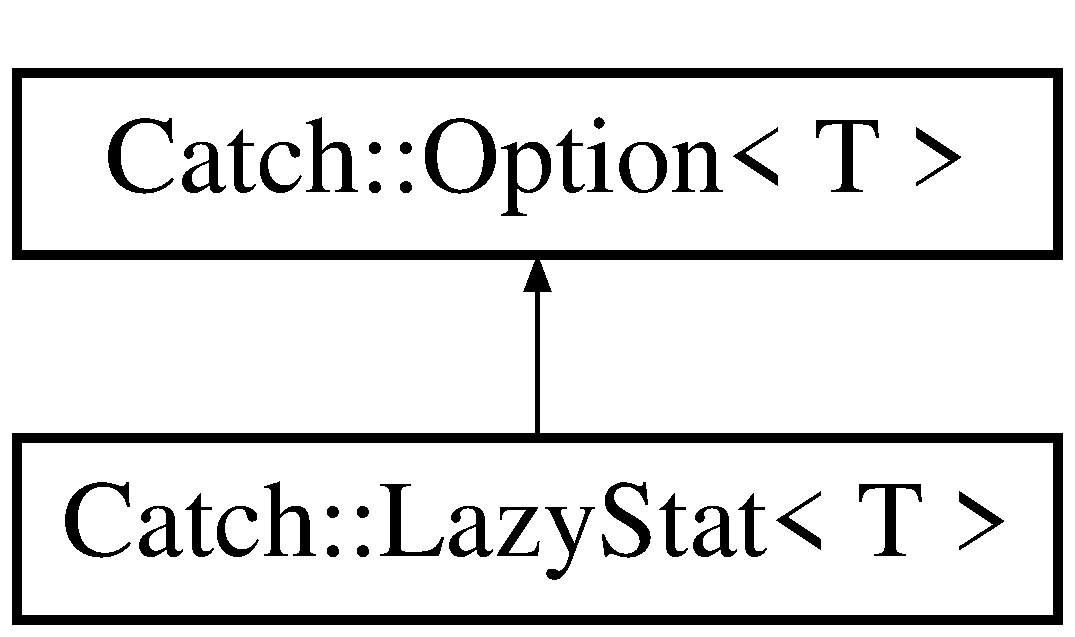
\includegraphics[height=2.000000cm]{struct_catch_1_1_lazy_stat}
\end{center}
\end{figure}
\subsection*{Public Member Functions}
\begin{DoxyCompactItemize}
\item 
\hypertarget{struct_catch_1_1_lazy_stat_af8e1c0c8b1b1975a515b190618f25b31}{\hyperlink{struct_catch_1_1_lazy_stat}{Lazy\-Stat} \& {\bfseries operator=} (T const \&\-\_\-value)}\label{struct_catch_1_1_lazy_stat_af8e1c0c8b1b1975a515b190618f25b31}

\item 
\hypertarget{struct_catch_1_1_lazy_stat_a535947bbc846868903cc960e747d9e03}{void {\bfseries reset} ()}\label{struct_catch_1_1_lazy_stat_a535947bbc846868903cc960e747d9e03}

\end{DoxyCompactItemize}
\subsection*{Public Attributes}
\begin{DoxyCompactItemize}
\item 
\hypertarget{struct_catch_1_1_lazy_stat_a3f68d716a1e972df47dc43b4d402124a}{bool {\bfseries used}}\label{struct_catch_1_1_lazy_stat_a3f68d716a1e972df47dc43b4d402124a}

\end{DoxyCompactItemize}


The documentation for this struct was generated from the following file\-:\begin{DoxyCompactItemize}
\item 
Catch.\-h\end{DoxyCompactItemize}

\hypertarget{class_l_l_parser}{\section{L\-L\-Parser Class Reference}
\label{class_l_l_parser}\index{L\-L\-Parser@{L\-L\-Parser}}
}


Class representing an L\-L Parser.  




{\ttfamily \#include $<$L\-L\-Parser.\-h$>$}

\subsection*{Public Member Functions}
\begin{DoxyCompactItemize}
\item 
\hyperlink{class_l_l_parser_afcc6a86b5054cedcdab1e682885103cb}{L\-L\-Parser} (const std\-::set$<$ char $>$ \&C\-F\-G\-Terminals, const std\-::set$<$ char $>$ \&C\-F\-G\-Variables, const std\-::multimap$<$ char, Symbol\-String $>$ \&C\-F\-G\-Productions, const char \&C\-F\-G\-Startsymbol, const unsigned int lookahead)
\begin{DoxyCompactList}\small\item\em Constructor, constructs an L\-L Parser from the given elements of a context free grammar. \end{DoxyCompactList}\item 
\hyperlink{class_l_l_parser_ac1f82371afde6215cdb47226317f8a64}{L\-L\-Parser} (const \hyperlink{class_c_f_g}{C\-F\-G} \&grammar, const unsigned int lookahead)
\begin{DoxyCompactList}\small\item\em Constructor, constructs an L\-L Parser for the given context free grammar. \end{DoxyCompactList}\item 
bool \hyperlink{class_l_l_parser_a3c849d307e60f966469d21c76f7ddc58}{process} (const std\-::string \&input) const 
\begin{DoxyCompactList}\small\item\em Process an input string through the L\-L Parser. \end{DoxyCompactList}\item 
\hypertarget{class_l_l_parser_afcc3d3e47b886797f852c50c705ffb5d}{virtual \hyperlink{class_l_l_parser_afcc3d3e47b886797f852c50c705ffb5d}{$\sim$\-L\-L\-Parser} ()}\label{class_l_l_parser_afcc3d3e47b886797f852c50c705ffb5d}

\begin{DoxyCompactList}\small\item\em Destructor. \end{DoxyCompactList}\end{DoxyCompactItemize}
\subsection*{Friends}
\begin{DoxyCompactItemize}
\item 
std\-::ostream \& \hyperlink{class_l_l_parser_adc9e5a8ce5b04aeca440293c75fdff75}{operator$<$$<$} (std\-::ostream \&stream, const \hyperlink{class_l_l_parser}{L\-L\-Parser} \&obj)
\begin{DoxyCompactList}\small\item\em Prints the parse table to the given output stream. \end{DoxyCompactList}\end{DoxyCompactItemize}


\subsection{Detailed Description}
Class representing an L\-L Parser. 

\subsection{Constructor \& Destructor Documentation}
\hypertarget{class_l_l_parser_afcc6a86b5054cedcdab1e682885103cb}{\index{L\-L\-Parser@{L\-L\-Parser}!L\-L\-Parser@{L\-L\-Parser}}
\index{L\-L\-Parser@{L\-L\-Parser}!LLParser@{L\-L\-Parser}}
\subsubsection[{L\-L\-Parser}]{\setlength{\rightskip}{0pt plus 5cm}L\-L\-Parser\-::\-L\-L\-Parser (
\begin{DoxyParamCaption}
\item[{const std\-::set$<$ char $>$ \&}]{C\-F\-G\-Terminals, }
\item[{const std\-::set$<$ char $>$ \&}]{C\-F\-G\-Variables, }
\item[{const std\-::multimap$<$ char, Symbol\-String $>$ \&}]{C\-F\-G\-Productions, }
\item[{const char \&}]{C\-F\-G\-Startsymbol, }
\item[{const unsigned int}]{lookahead}
\end{DoxyParamCaption}
)}}\label{class_l_l_parser_afcc6a86b5054cedcdab1e682885103cb}


Constructor, constructs an L\-L Parser from the given elements of a context free grammar. 


\begin{DoxyParams}{Parameters}
{\em C\-F\-G\-Terminals} & A set containing the terminals of the \hyperlink{class_c_f_g}{C\-F\-G} \\
\hline
{\em C\-F\-G\-Variables} & A set containing the variables of the \hyperlink{class_c_f_g}{C\-F\-G} \\
\hline
{\em C\-F\-G\-Productions} & A multimap that maps a variable to an symbol\-String \\
\hline
{\em C\-F\-G\-Startsymbol} & The startsymbol for the \hyperlink{class_c_f_g}{C\-F\-G} \\
\hline
{\em lookahead} & The size of the lookahead (k)\\
\hline
\end{DoxyParams}

\begin{DoxyExceptions}{Exceptions}
{\em invalid\-\_\-argument} & Throws this exception when the Parser can't be contructed \\
\hline
\end{DoxyExceptions}
\hypertarget{class_l_l_parser_ac1f82371afde6215cdb47226317f8a64}{\index{L\-L\-Parser@{L\-L\-Parser}!L\-L\-Parser@{L\-L\-Parser}}
\index{L\-L\-Parser@{L\-L\-Parser}!LLParser@{L\-L\-Parser}}
\subsubsection[{L\-L\-Parser}]{\setlength{\rightskip}{0pt plus 5cm}L\-L\-Parser\-::\-L\-L\-Parser (
\begin{DoxyParamCaption}
\item[{const {\bf C\-F\-G} \&}]{grammar, }
\item[{const unsigned int}]{lookahead}
\end{DoxyParamCaption}
)}}\label{class_l_l_parser_ac1f82371afde6215cdb47226317f8a64}


Constructor, constructs an L\-L Parser for the given context free grammar. 


\begin{DoxyParams}{Parameters}
{\em grammar} & A context free grammar as a base for this L\-L Parser \\
\hline
{\em lookahead} & The size of the lookahead (k)\\
\hline
\end{DoxyParams}

\begin{DoxyExceptions}{Exceptions}
{\em invalid\-\_\-argument} & Throws this exception when the Parser can't be contructed \\
\hline
\end{DoxyExceptions}


\subsection{Member Function Documentation}
\hypertarget{class_l_l_parser_a3c849d307e60f966469d21c76f7ddc58}{\index{L\-L\-Parser@{L\-L\-Parser}!process@{process}}
\index{process@{process}!LLParser@{L\-L\-Parser}}
\subsubsection[{process}]{\setlength{\rightskip}{0pt plus 5cm}bool L\-L\-Parser\-::process (
\begin{DoxyParamCaption}
\item[{const std\-::string \&}]{input}
\end{DoxyParamCaption}
) const}}\label{class_l_l_parser_a3c849d307e60f966469d21c76f7ddc58}


Process an input string through the L\-L Parser. 


\begin{DoxyParams}{Parameters}
{\em input} & The string to be processed by the L\-L Parser\\
\hline
\end{DoxyParams}
\begin{DoxyReturn}{Returns}
A bool telling if the Parser accepted 
\end{DoxyReturn}


\subsection{Friends And Related Function Documentation}
\hypertarget{class_l_l_parser_adc9e5a8ce5b04aeca440293c75fdff75}{\index{L\-L\-Parser@{L\-L\-Parser}!operator$<$$<$@{operator$<$$<$}}
\index{operator$<$$<$@{operator$<$$<$}!LLParser@{L\-L\-Parser}}
\subsubsection[{operator$<$$<$}]{\setlength{\rightskip}{0pt plus 5cm}std\-::ostream\& operator$<$$<$ (
\begin{DoxyParamCaption}
\item[{std\-::ostream \&}]{stream, }
\item[{const {\bf L\-L\-Parser} \&}]{obj}
\end{DoxyParamCaption}
)\hspace{0.3cm}{\ttfamily [friend]}}}\label{class_l_l_parser_adc9e5a8ce5b04aeca440293c75fdff75}


Prints the parse table to the given output stream. 


\begin{DoxyParams}{Parameters}
{\em stream} & The output stream \\
\hline
{\em obj} & The parser\\
\hline
\end{DoxyParams}
\begin{DoxyReturn}{Returns}
The output stream. 
\end{DoxyReturn}


The documentation for this class was generated from the following files\-:\begin{DoxyCompactItemize}
\item 
L\-L\-Parser.\-h\item 
L\-L\-Parser.\-cpp\end{DoxyCompactItemize}

\hypertarget{class_l_l_table}{\section{L\-L\-Table Class Reference}
\label{class_l_l_table}\index{L\-L\-Table@{L\-L\-Table}}
}


Class representing an L\-L Parse Table.  




{\ttfamily \#include $<$L\-L\-Parser.\-h$>$}

\subsection*{Public Member Functions}
\begin{DoxyCompactItemize}
\item 
\hyperlink{class_l_l_table_a6c4e8032c91212be9d5b4cf22fc69c0d}{L\-L\-Table} (const std\-::set$<$ char $>$ \&C\-F\-G\-Terminals, const std\-::set$<$ char $>$ \&C\-F\-G\-Variables, const std\-::multimap$<$ char, Symbol\-String $>$ \&C\-F\-G\-Productions, const unsigned int dimension)
\begin{DoxyCompactList}\small\item\em Constructor, constructs an L\-L Parse Table from the given elements of a context free grammar. \end{DoxyCompactList}\item 
\hyperlink{class_l_l_table_a4aacfa72d10dcbcba22d42e08408ba91}{L\-L\-Table} (const \hyperlink{class_c_f_g}{C\-F\-G} \&grammar, const unsigned int dimension)
\begin{DoxyCompactList}\small\item\em Constructor, constructs an L\-L Parse Table for the given context free grammar. \end{DoxyCompactList}\item 
Symbol\-String \hyperlink{class_l_l_table_a403059b89fd2f82f2b4d83cca658ef08}{process} (const char \&top\-Stack, const Symbol\-String \&remaining\-Input) const 
\begin{DoxyCompactList}\small\item\em Process one input symbol of the remaining input string. \end{DoxyCompactList}\item 
\hypertarget{class_l_l_table_a37eed818542510ffc9ce790d2c7e7e84}{virtual \hyperlink{class_l_l_table_a37eed818542510ffc9ce790d2c7e7e84}{$\sim$\-L\-L\-Table} ()}\label{class_l_l_table_a37eed818542510ffc9ce790d2c7e7e84}

\begin{DoxyCompactList}\small\item\em Destructor. \end{DoxyCompactList}\item 
std\-::string \hyperlink{class_l_l_table_a01eaf21e0fefb3978d7276b082dba225}{to\-String} (const std\-::set$<$ char $>$ \&C\-F\-G\-Terminals, const std\-::set$<$ char $>$ \&C\-F\-G\-Variables) const 
\begin{DoxyCompactList}\small\item\em Returns a string representation of the parse table. \end{DoxyCompactList}\end{DoxyCompactItemize}
\subsection*{Static Public Member Functions}
\begin{DoxyCompactItemize}
\item 
static void \hyperlink{class_l_l_table_aba85aa55846e156f5ea5ca631da6c51c}{enumerate} (std\-::vector$<$ Symbol\-String $>$ \&result, std\-::vector$<$ Symbol\-String $>$ \&terminals, unsigned int length)
\begin{DoxyCompactList}\small\item\em Enumerates all possible combinations of the given terminals. \end{DoxyCompactList}\end{DoxyCompactItemize}


\subsection{Detailed Description}
Class representing an L\-L Parse Table. 

\subsection{Constructor \& Destructor Documentation}
\hypertarget{class_l_l_table_a6c4e8032c91212be9d5b4cf22fc69c0d}{\index{L\-L\-Table@{L\-L\-Table}!L\-L\-Table@{L\-L\-Table}}
\index{L\-L\-Table@{L\-L\-Table}!LLTable@{L\-L\-Table}}
\subsubsection[{L\-L\-Table}]{\setlength{\rightskip}{0pt plus 5cm}L\-L\-Table\-::\-L\-L\-Table (
\begin{DoxyParamCaption}
\item[{const std\-::set$<$ char $>$ \&}]{C\-F\-G\-Terminals, }
\item[{const std\-::set$<$ char $>$ \&}]{C\-F\-G\-Variables, }
\item[{const std\-::multimap$<$ char, Symbol\-String $>$ \&}]{C\-F\-G\-Productions, }
\item[{const unsigned int}]{dimension}
\end{DoxyParamCaption}
)}}\label{class_l_l_table_a6c4e8032c91212be9d5b4cf22fc69c0d}


Constructor, constructs an L\-L Parse Table from the given elements of a context free grammar. 


\begin{DoxyParams}{Parameters}
{\em C\-F\-G\-Terminals} & A set containing the terminals of the \hyperlink{class_c_f_g}{C\-F\-G} \\
\hline
{\em C\-F\-G\-Variables} & A set containing the variables of the \hyperlink{class_c_f_g}{C\-F\-G} \\
\hline
{\em C\-F\-G\-Productions} & A multimap that maps a variable to an symbol\-String \\
\hline
{\em dimension} & The dimension of the table, thus the size of the lookahead (k)\\
\hline
\end{DoxyParams}

\begin{DoxyExceptions}{Exceptions}
{\em invalid\-\_\-argument} & Throws this exception when the Table can't be contructed \\
\hline
\end{DoxyExceptions}
\hypertarget{class_l_l_table_a4aacfa72d10dcbcba22d42e08408ba91}{\index{L\-L\-Table@{L\-L\-Table}!L\-L\-Table@{L\-L\-Table}}
\index{L\-L\-Table@{L\-L\-Table}!LLTable@{L\-L\-Table}}
\subsubsection[{L\-L\-Table}]{\setlength{\rightskip}{0pt plus 5cm}L\-L\-Table\-::\-L\-L\-Table (
\begin{DoxyParamCaption}
\item[{const {\bf C\-F\-G} \&}]{grammar, }
\item[{const unsigned int}]{dimension}
\end{DoxyParamCaption}
)}}\label{class_l_l_table_a4aacfa72d10dcbcba22d42e08408ba91}


Constructor, constructs an L\-L Parse Table for the given context free grammar. 


\begin{DoxyParams}{Parameters}
{\em grammar} & A context free grammar as a base for this L\-L Parser \\
\hline
{\em dimension} & The dimension of the table, thus the size of the lookahead (k)\\
\hline
\end{DoxyParams}

\begin{DoxyExceptions}{Exceptions}
{\em invalid\-\_\-argument} & Throws this exception when the Table can't be contructed \\
\hline
\end{DoxyExceptions}


\subsection{Member Function Documentation}
\hypertarget{class_l_l_table_aba85aa55846e156f5ea5ca631da6c51c}{\index{L\-L\-Table@{L\-L\-Table}!enumerate@{enumerate}}
\index{enumerate@{enumerate}!LLTable@{L\-L\-Table}}
\subsubsection[{enumerate}]{\setlength{\rightskip}{0pt plus 5cm}void L\-L\-Table\-::enumerate (
\begin{DoxyParamCaption}
\item[{std\-::vector$<$ Symbol\-String $>$ \&}]{result, }
\item[{std\-::vector$<$ Symbol\-String $>$ \&}]{terminals, }
\item[{unsigned int}]{length}
\end{DoxyParamCaption}
)\hspace{0.3cm}{\ttfamily [static]}}}\label{class_l_l_table_aba85aa55846e156f5ea5ca631da6c51c}


Enumerates all possible combinations of the given terminals. 


\begin{DoxyParams}{Parameters}
{\em result} & Container for all combinations \\
\hline
{\em terminals} & All terminals that can be used in a combination \\
\hline
{\em length} & The desired length of the combinations \\
\hline
\end{DoxyParams}
\hypertarget{class_l_l_table_a403059b89fd2f82f2b4d83cca658ef08}{\index{L\-L\-Table@{L\-L\-Table}!process@{process}}
\index{process@{process}!LLTable@{L\-L\-Table}}
\subsubsection[{process}]{\setlength{\rightskip}{0pt plus 5cm}Symbol\-String L\-L\-Table\-::process (
\begin{DoxyParamCaption}
\item[{const char \&}]{top\-Stack, }
\item[{const Symbol\-String \&}]{remaining\-Input}
\end{DoxyParamCaption}
) const}}\label{class_l_l_table_a403059b89fd2f82f2b4d83cca658ef08}


Process one input symbol of the remaining input string. 


\begin{DoxyParams}{Parameters}
{\em top\-Stack} & The variable at the top of the stack \\
\hline
{\em remaining\-Input} & The remaining part of the input string\\
\hline
\end{DoxyParams}
\begin{DoxyPrecond}{Precondition}
top\-Stack is an element of C\-F\-G\-Variables
\end{DoxyPrecond}

\begin{DoxyExceptions}{Exceptions}
{\em runtime\-\_\-error} & Throws this exception when the remaining input string results in an error\\
\hline
\end{DoxyExceptions}
\begin{DoxyReturn}{Returns}
The right side of the used production rule. 
\end{DoxyReturn}
\hypertarget{class_l_l_table_a01eaf21e0fefb3978d7276b082dba225}{\index{L\-L\-Table@{L\-L\-Table}!to\-String@{to\-String}}
\index{to\-String@{to\-String}!LLTable@{L\-L\-Table}}
\subsubsection[{to\-String}]{\setlength{\rightskip}{0pt plus 5cm}std\-::string L\-L\-Table\-::to\-String (
\begin{DoxyParamCaption}
\item[{const std\-::set$<$ char $>$ \&}]{C\-F\-G\-Terminals, }
\item[{const std\-::set$<$ char $>$ \&}]{C\-F\-G\-Variables}
\end{DoxyParamCaption}
) const}}\label{class_l_l_table_a01eaf21e0fefb3978d7276b082dba225}


Returns a string representation of the parse table. 


\begin{DoxyParams}{Parameters}
{\em C\-F\-G\-Terminals} & A set containing the terminals of the \hyperlink{class_c_f_g}{C\-F\-G} \\
\hline
{\em C\-F\-G\-Variables} & A set containing the variables of the \hyperlink{class_c_f_g}{C\-F\-G}\\
\hline
\end{DoxyParams}
\begin{DoxyReturn}{Returns}
String representation. 
\end{DoxyReturn}


The documentation for this class was generated from the following files\-:\begin{DoxyCompactItemize}
\item 
L\-L\-Parser.\-h\item 
L\-L\-Parser.\-cpp\end{DoxyCompactItemize}

\hypertarget{struct_catch_1_1_matchers_1_1_impl_1_1_matcher}{\section{Catch\-:\-:Matchers\-:\-:Impl\-:\-:Matcher$<$ Expression\-T $>$ Struct Template Reference}
\label{struct_catch_1_1_matchers_1_1_impl_1_1_matcher}\index{Catch\-::\-Matchers\-::\-Impl\-::\-Matcher$<$ Expression\-T $>$@{Catch\-::\-Matchers\-::\-Impl\-::\-Matcher$<$ Expression\-T $>$}}
}
Inheritance diagram for Catch\-:\-:Matchers\-:\-:Impl\-:\-:Matcher$<$ Expression\-T $>$\-:\begin{figure}[H]
\begin{center}
\leavevmode
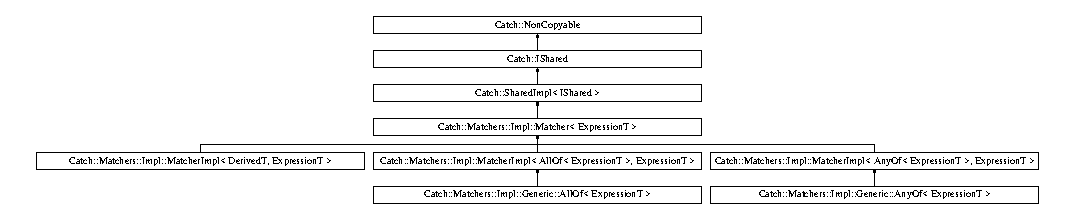
\includegraphics[height=2.505593cm]{struct_catch_1_1_matchers_1_1_impl_1_1_matcher}
\end{center}
\end{figure}
\subsection*{Public Types}
\begin{DoxyCompactItemize}
\item 
\hypertarget{struct_catch_1_1_matchers_1_1_impl_1_1_matcher_a7f5068cbacd1eed06cf243e63446e7e1}{typedef Expression\-T {\bfseries Expression\-Type}}\label{struct_catch_1_1_matchers_1_1_impl_1_1_matcher_a7f5068cbacd1eed06cf243e63446e7e1}

\end{DoxyCompactItemize}
\subsection*{Public Member Functions}
\begin{DoxyCompactItemize}
\item 
\hypertarget{struct_catch_1_1_matchers_1_1_impl_1_1_matcher_a9d31e5018fea24efa08c3cbf5aa4475d}{virtual \hyperlink{class_catch_1_1_ptr}{Ptr}$<$ \hyperlink{struct_catch_1_1_matchers_1_1_impl_1_1_matcher}{Matcher} $>$ {\bfseries clone} () const =0}\label{struct_catch_1_1_matchers_1_1_impl_1_1_matcher_a9d31e5018fea24efa08c3cbf5aa4475d}

\item 
\hypertarget{struct_catch_1_1_matchers_1_1_impl_1_1_matcher_a8c1c5511ce1f3738a45e6901b558f583}{virtual bool {\bfseries match} (Expression\-T const \&expr) const =0}\label{struct_catch_1_1_matchers_1_1_impl_1_1_matcher_a8c1c5511ce1f3738a45e6901b558f583}

\item 
\hypertarget{struct_catch_1_1_matchers_1_1_impl_1_1_matcher_a091bcc37e589967d7e10fc7790d820e2}{virtual std\-::string {\bfseries to\-String} () const =0}\label{struct_catch_1_1_matchers_1_1_impl_1_1_matcher_a091bcc37e589967d7e10fc7790d820e2}

\end{DoxyCompactItemize}
\subsection*{Additional Inherited Members}


The documentation for this struct was generated from the following file\-:\begin{DoxyCompactItemize}
\item 
Catch.\-h\end{DoxyCompactItemize}

\hypertarget{struct_catch_1_1_matchers_1_1_impl_1_1_matcher_impl}{\section{Catch\-:\-:Matchers\-:\-:Impl\-:\-:Matcher\-Impl$<$ Derived\-T, Expression\-T $>$ Struct Template Reference}
\label{struct_catch_1_1_matchers_1_1_impl_1_1_matcher_impl}\index{Catch\-::\-Matchers\-::\-Impl\-::\-Matcher\-Impl$<$ Derived\-T, Expression\-T $>$@{Catch\-::\-Matchers\-::\-Impl\-::\-Matcher\-Impl$<$ Derived\-T, Expression\-T $>$}}
}
Inheritance diagram for Catch\-:\-:Matchers\-:\-:Impl\-:\-:Matcher\-Impl$<$ Derived\-T, Expression\-T $>$\-:\begin{figure}[H]
\begin{center}
\leavevmode
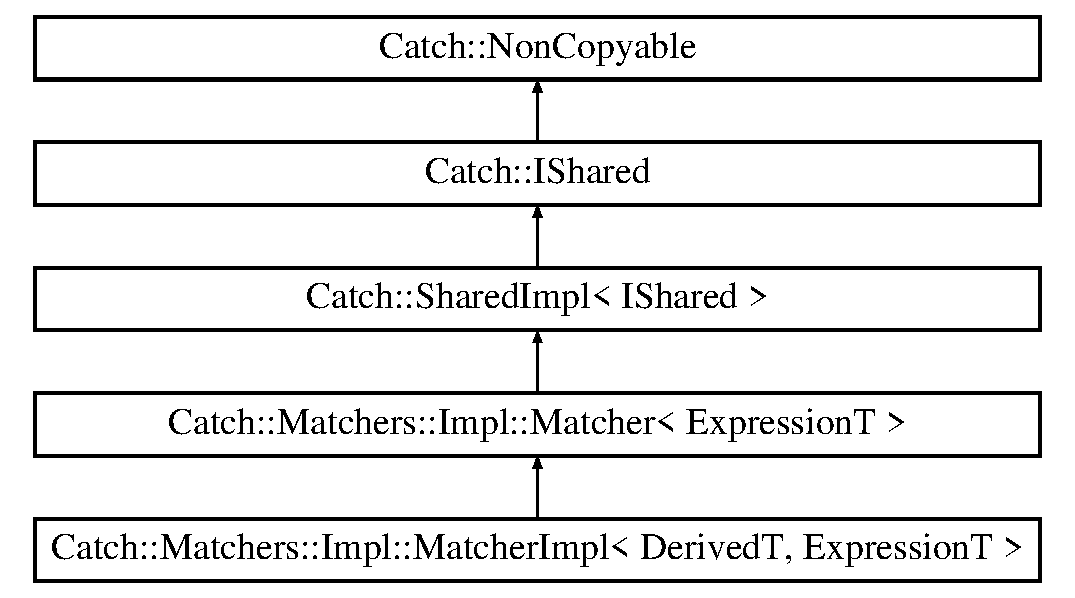
\includegraphics[height=5.000000cm]{struct_catch_1_1_matchers_1_1_impl_1_1_matcher_impl}
\end{center}
\end{figure}
\subsection*{Public Member Functions}
\begin{DoxyCompactItemize}
\item 
\hypertarget{struct_catch_1_1_matchers_1_1_impl_1_1_matcher_impl_afe2e10779f91394f80ff5c894fb1bfab}{virtual \hyperlink{class_catch_1_1_ptr}{Ptr}$<$ \hyperlink{struct_catch_1_1_matchers_1_1_impl_1_1_matcher}{Matcher}\\*
$<$ Expression\-T $>$ $>$ {\bfseries clone} () const }\label{struct_catch_1_1_matchers_1_1_impl_1_1_matcher_impl_afe2e10779f91394f80ff5c894fb1bfab}

\end{DoxyCompactItemize}
\subsection*{Additional Inherited Members}


The documentation for this struct was generated from the following file\-:\begin{DoxyCompactItemize}
\item 
Catch.\-h\end{DoxyCompactItemize}

\hypertarget{struct_catch_1_1_message_builder}{\section{Catch\-:\-:Message\-Builder Struct Reference}
\label{struct_catch_1_1_message_builder}\index{Catch\-::\-Message\-Builder@{Catch\-::\-Message\-Builder}}
}
\subsection*{Public Member Functions}
\begin{DoxyCompactItemize}
\item 
\hypertarget{struct_catch_1_1_message_builder_ab0c6378e722680bf58852c6ee2b6e724}{{\bfseries Message\-Builder} (std\-::string const \&macro\-Name, \hyperlink{struct_catch_1_1_source_line_info}{Source\-Line\-Info} const \&line\-Info, Result\-Was\-::\-Of\-Type type)}\label{struct_catch_1_1_message_builder_ab0c6378e722680bf58852c6ee2b6e724}

\item 
\hypertarget{struct_catch_1_1_message_builder_a20fa48d069b20dddcc2d3df8abb123c1}{{\footnotesize template$<$typename T $>$ }\\\hyperlink{struct_catch_1_1_message_builder}{Message\-Builder} \& {\bfseries operator$<$$<$} (T const \&value)}\label{struct_catch_1_1_message_builder_a20fa48d069b20dddcc2d3df8abb123c1}

\end{DoxyCompactItemize}
\subsection*{Public Attributes}
\begin{DoxyCompactItemize}
\item 
\hypertarget{struct_catch_1_1_message_builder_a979f1c2b36d78f80ee275bfa5ba0209f}{\hyperlink{struct_catch_1_1_message_info}{Message\-Info} {\bfseries m\-\_\-info}}\label{struct_catch_1_1_message_builder_a979f1c2b36d78f80ee275bfa5ba0209f}

\item 
\hypertarget{struct_catch_1_1_message_builder_a6488ab0cc4ea52affc9c0612c7c5df6b}{std\-::ostringstream {\bfseries m\-\_\-stream}}\label{struct_catch_1_1_message_builder_a6488ab0cc4ea52affc9c0612c7c5df6b}

\end{DoxyCompactItemize}


The documentation for this struct was generated from the following file\-:\begin{DoxyCompactItemize}
\item 
Catch.\-h\end{DoxyCompactItemize}

\hypertarget{struct_catch_1_1_message_info}{\section{Catch\-:\-:Message\-Info Struct Reference}
\label{struct_catch_1_1_message_info}\index{Catch\-::\-Message\-Info@{Catch\-::\-Message\-Info}}
}
\subsection*{Public Member Functions}
\begin{DoxyCompactItemize}
\item 
\hypertarget{struct_catch_1_1_message_info_a2e336c33ebef7af3c1bbae6a56e14f8a}{{\bfseries Message\-Info} (std\-::string const \&\-\_\-macro\-Name, \hyperlink{struct_catch_1_1_source_line_info}{Source\-Line\-Info} const \&\-\_\-line\-Info, Result\-Was\-::\-Of\-Type \-\_\-type)}\label{struct_catch_1_1_message_info_a2e336c33ebef7af3c1bbae6a56e14f8a}

\item 
\hypertarget{struct_catch_1_1_message_info_a30fe117138e568c5a9dfdabb7de6e790}{bool {\bfseries operator==} (\hyperlink{struct_catch_1_1_message_info}{Message\-Info} const \&other) const }\label{struct_catch_1_1_message_info_a30fe117138e568c5a9dfdabb7de6e790}

\item 
\hypertarget{struct_catch_1_1_message_info_a7a2b1ec3772cd35176e2ee25a94be16a}{bool {\bfseries operator$<$} (\hyperlink{struct_catch_1_1_message_info}{Message\-Info} const \&other) const }\label{struct_catch_1_1_message_info_a7a2b1ec3772cd35176e2ee25a94be16a}

\end{DoxyCompactItemize}
\subsection*{Public Attributes}
\begin{DoxyCompactItemize}
\item 
\hypertarget{struct_catch_1_1_message_info_a156ade4b3cc731f6ec7b542ae47ba8e3}{std\-::string {\bfseries macro\-Name}}\label{struct_catch_1_1_message_info_a156ade4b3cc731f6ec7b542ae47ba8e3}

\item 
\hypertarget{struct_catch_1_1_message_info_a985165328723e599696ebd8e43195cc5}{\hyperlink{struct_catch_1_1_source_line_info}{Source\-Line\-Info} {\bfseries line\-Info}}\label{struct_catch_1_1_message_info_a985165328723e599696ebd8e43195cc5}

\item 
\hypertarget{struct_catch_1_1_message_info_ae928b9117465c696e45951d9d0284e78}{Result\-Was\-::\-Of\-Type {\bfseries type}}\label{struct_catch_1_1_message_info_ae928b9117465c696e45951d9d0284e78}

\item 
\hypertarget{struct_catch_1_1_message_info_ab6cd06e050bf426c6577502a5c50e256}{std\-::string {\bfseries message}}\label{struct_catch_1_1_message_info_ab6cd06e050bf426c6577502a5c50e256}

\item 
\hypertarget{struct_catch_1_1_message_info_a7f4f57ea21e50160adefce7b68a781d6}{unsigned int {\bfseries sequence}}\label{struct_catch_1_1_message_info_a7f4f57ea21e50160adefce7b68a781d6}

\end{DoxyCompactItemize}


The documentation for this struct was generated from the following file\-:\begin{DoxyCompactItemize}
\item 
Catch.\-h\end{DoxyCompactItemize}

\hypertarget{class_catch_1_1_method_test_case}{\section{Catch\-:\-:Method\-Test\-Case$<$ C $>$ Class Template Reference}
\label{class_catch_1_1_method_test_case}\index{Catch\-::\-Method\-Test\-Case$<$ C $>$@{Catch\-::\-Method\-Test\-Case$<$ C $>$}}
}
Inheritance diagram for Catch\-:\-:Method\-Test\-Case$<$ C $>$\-:\begin{figure}[H]
\begin{center}
\leavevmode
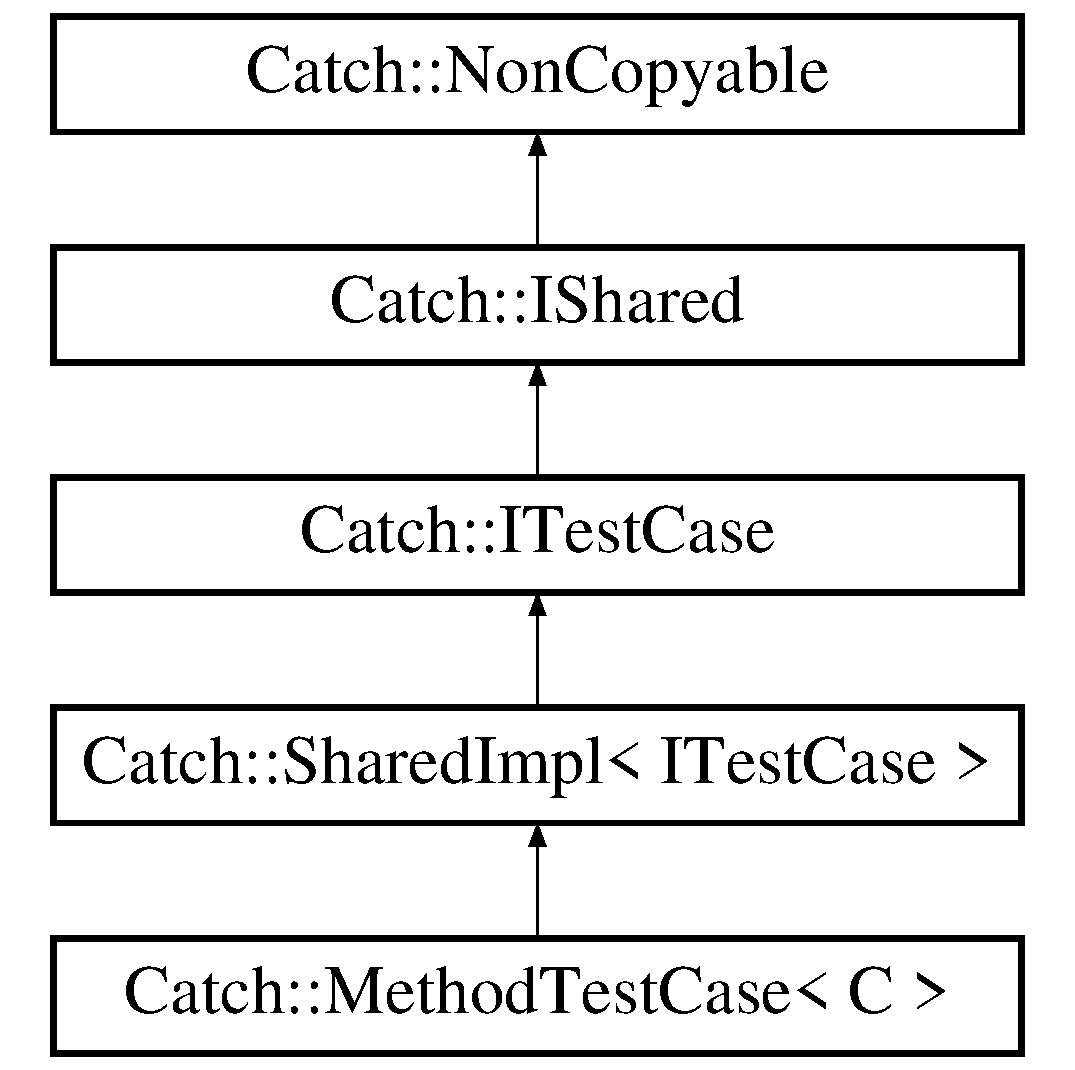
\includegraphics[height=5.000000cm]{class_catch_1_1_method_test_case}
\end{center}
\end{figure}
\subsection*{Public Member Functions}
\begin{DoxyCompactItemize}
\item 
\hypertarget{class_catch_1_1_method_test_case_a7b043b85dae371358255dd9dc6582e7b}{{\bfseries Method\-Test\-Case} (void(C\-::$\ast$method)())}\label{class_catch_1_1_method_test_case_a7b043b85dae371358255dd9dc6582e7b}

\item 
\hypertarget{class_catch_1_1_method_test_case_a39cc4b760dd71adc3f7550bc1e7eb697}{virtual void {\bfseries invoke} () const }\label{class_catch_1_1_method_test_case_a39cc4b760dd71adc3f7550bc1e7eb697}

\end{DoxyCompactItemize}
\subsection*{Additional Inherited Members}


The documentation for this class was generated from the following file\-:\begin{DoxyCompactItemize}
\item 
Catch.\-h\end{DoxyCompactItemize}

\hypertarget{struct_catch_1_1_name_and_desc}{\section{Catch\-:\-:Name\-And\-Desc Struct Reference}
\label{struct_catch_1_1_name_and_desc}\index{Catch\-::\-Name\-And\-Desc@{Catch\-::\-Name\-And\-Desc}}
}
\subsection*{Public Member Functions}
\begin{DoxyCompactItemize}
\item 
\hypertarget{struct_catch_1_1_name_and_desc_a189ceb9942fb5f6635140d6a09fc843a}{{\bfseries Name\-And\-Desc} (const char $\ast$\-\_\-name=\char`\"{}\char`\"{}, const char $\ast$\-\_\-description=\char`\"{}\char`\"{})}\label{struct_catch_1_1_name_and_desc_a189ceb9942fb5f6635140d6a09fc843a}

\end{DoxyCompactItemize}
\subsection*{Public Attributes}
\begin{DoxyCompactItemize}
\item 
\hypertarget{struct_catch_1_1_name_and_desc_a374b4ed8be3cf98be20ebde5273bde51}{const char $\ast$ {\bfseries name}}\label{struct_catch_1_1_name_and_desc_a374b4ed8be3cf98be20ebde5273bde51}

\item 
\hypertarget{struct_catch_1_1_name_and_desc_a3463a23ff65ce494fc380452b57b7970}{const char $\ast$ {\bfseries description}}\label{struct_catch_1_1_name_and_desc_a3463a23ff65ce494fc380452b57b7970}

\end{DoxyCompactItemize}


The documentation for this struct was generated from the following file\-:\begin{DoxyCompactItemize}
\item 
Catch.\-h\end{DoxyCompactItemize}

\hypertarget{struct_catch_1_1_cumulative_reporter_base_1_1_node}{\section{Catch\-:\-:Cumulative\-Reporter\-Base\-:\-:Node$<$ T, Child\-Node\-T $>$ Struct Template Reference}
\label{struct_catch_1_1_cumulative_reporter_base_1_1_node}\index{Catch\-::\-Cumulative\-Reporter\-Base\-::\-Node$<$ T, Child\-Node\-T $>$@{Catch\-::\-Cumulative\-Reporter\-Base\-::\-Node$<$ T, Child\-Node\-T $>$}}
}
Inheritance diagram for Catch\-:\-:Cumulative\-Reporter\-Base\-:\-:Node$<$ T, Child\-Node\-T $>$\-:\begin{figure}[H]
\begin{center}
\leavevmode
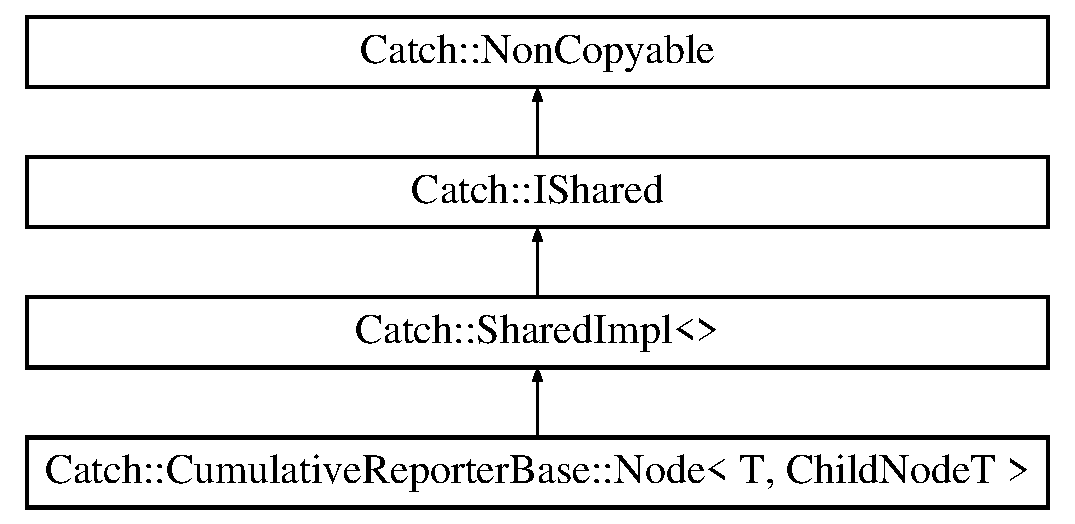
\includegraphics[height=4.000000cm]{struct_catch_1_1_cumulative_reporter_base_1_1_node}
\end{center}
\end{figure}
\subsection*{Public Types}
\begin{DoxyCompactItemize}
\item 
\hypertarget{struct_catch_1_1_cumulative_reporter_base_1_1_node_ad410701d72466c05acf86956aabafaf1}{typedef std\-::vector$<$ \hyperlink{class_catch_1_1_ptr}{Ptr}\\*
$<$ Child\-Node\-T $>$ $>$ {\bfseries Child\-Nodes}}\label{struct_catch_1_1_cumulative_reporter_base_1_1_node_ad410701d72466c05acf86956aabafaf1}

\end{DoxyCompactItemize}
\subsection*{Public Member Functions}
\begin{DoxyCompactItemize}
\item 
\hypertarget{struct_catch_1_1_cumulative_reporter_base_1_1_node_afff50af7c9f08e9fef089baa7c948096}{{\bfseries Node} (T const \&\-\_\-value)}\label{struct_catch_1_1_cumulative_reporter_base_1_1_node_afff50af7c9f08e9fef089baa7c948096}

\end{DoxyCompactItemize}
\subsection*{Public Attributes}
\begin{DoxyCompactItemize}
\item 
\hypertarget{struct_catch_1_1_cumulative_reporter_base_1_1_node_ac028cad2accba6cac30b92619bc8cfa0}{T {\bfseries value}}\label{struct_catch_1_1_cumulative_reporter_base_1_1_node_ac028cad2accba6cac30b92619bc8cfa0}

\item 
\hypertarget{struct_catch_1_1_cumulative_reporter_base_1_1_node_a7b123f17f6b77f5cd4e2f9c1325515a4}{Child\-Nodes {\bfseries children}}\label{struct_catch_1_1_cumulative_reporter_base_1_1_node_a7b123f17f6b77f5cd4e2f9c1325515a4}

\end{DoxyCompactItemize}


The documentation for this struct was generated from the following file\-:\begin{DoxyCompactItemize}
\item 
Catch.\-h\end{DoxyCompactItemize}

\hypertarget{class_catch_1_1_non_copyable}{\section{Catch\-:\-:Non\-Copyable Class Reference}
\label{class_catch_1_1_non_copyable}\index{Catch\-::\-Non\-Copyable@{Catch\-::\-Non\-Copyable}}
}
Inheritance diagram for Catch\-:\-:Non\-Copyable\-:\begin{figure}[H]
\begin{center}
\leavevmode
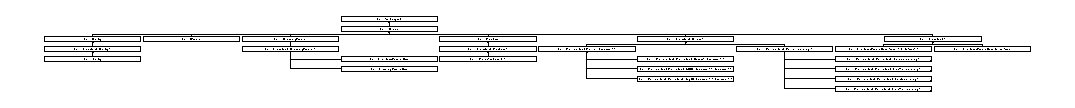
\includegraphics[height=1.002237cm]{class_catch_1_1_non_copyable}
\end{center}
\end{figure}


The documentation for this class was generated from the following file\-:\begin{DoxyCompactItemize}
\item 
Catch.\-h\end{DoxyCompactItemize}

\hypertarget{class_catch_1_1_not_implemented_exception}{\section{Catch\-:\-:Not\-Implemented\-Exception Class Reference}
\label{class_catch_1_1_not_implemented_exception}\index{Catch\-::\-Not\-Implemented\-Exception@{Catch\-::\-Not\-Implemented\-Exception}}
}
Inheritance diagram for Catch\-:\-:Not\-Implemented\-Exception\-:\begin{figure}[H]
\begin{center}
\leavevmode
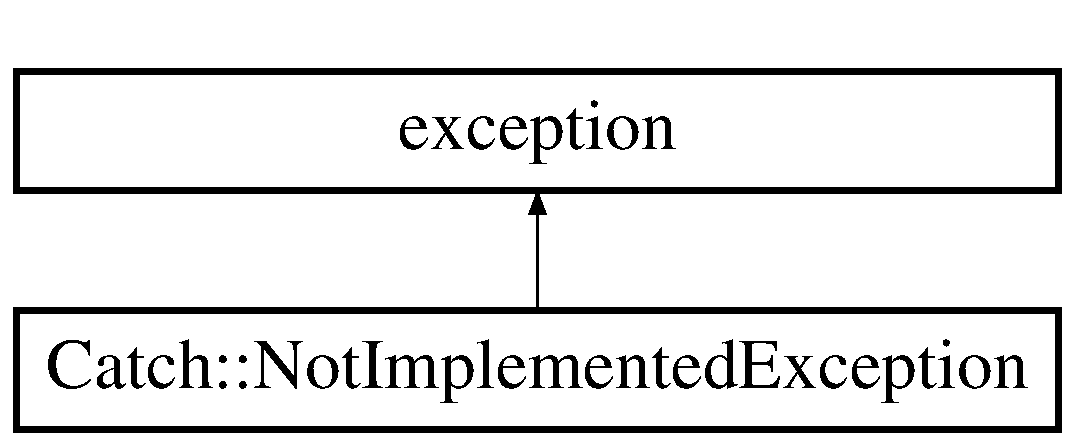
\includegraphics[height=2.000000cm]{class_catch_1_1_not_implemented_exception}
\end{center}
\end{figure}
\subsection*{Public Member Functions}
\begin{DoxyCompactItemize}
\item 
\hypertarget{class_catch_1_1_not_implemented_exception_ab4f0a5c39d8ffb72c664e2c07e180634}{{\bfseries Not\-Implemented\-Exception} (\hyperlink{struct_catch_1_1_source_line_info}{Source\-Line\-Info} const \&line\-Info)}\label{class_catch_1_1_not_implemented_exception_ab4f0a5c39d8ffb72c664e2c07e180634}

\item 
\hypertarget{class_catch_1_1_not_implemented_exception_a9d262173d2e1a5acccf8eb7b3a4859b6}{virtual const char $\ast$ {\bfseries what} () const   throw ()}\label{class_catch_1_1_not_implemented_exception_a9d262173d2e1a5acccf8eb7b3a4859b6}

\end{DoxyCompactItemize}


The documentation for this class was generated from the following file\-:\begin{DoxyCompactItemize}
\item 
Catch.\-h\end{DoxyCompactItemize}

\hypertarget{struct_catch_1_1_internal_1_1_operator_traits}{\section{Catch\-:\-:Internal\-:\-:Operator\-Traits$<$ Op $>$ Struct Template Reference}
\label{struct_catch_1_1_internal_1_1_operator_traits}\index{Catch\-::\-Internal\-::\-Operator\-Traits$<$ Op $>$@{Catch\-::\-Internal\-::\-Operator\-Traits$<$ Op $>$}}
}
\subsection*{Static Public Member Functions}
\begin{DoxyCompactItemize}
\item 
\hypertarget{struct_catch_1_1_internal_1_1_operator_traits_ac6d08082ea33348d42bc4ccbd6d07671}{static const char $\ast$ {\bfseries get\-Name} ()}\label{struct_catch_1_1_internal_1_1_operator_traits_ac6d08082ea33348d42bc4ccbd6d07671}

\end{DoxyCompactItemize}


The documentation for this struct was generated from the following file\-:\begin{DoxyCompactItemize}
\item 
Catch.\-h\end{DoxyCompactItemize}

\hypertarget{struct_catch_1_1_internal_1_1_operator_traits_3_01_is_equal_to_01_4}{\section{Catch\-:\-:Internal\-:\-:Operator\-Traits$<$ Is\-Equal\-To $>$ Struct Template Reference}
\label{struct_catch_1_1_internal_1_1_operator_traits_3_01_is_equal_to_01_4}\index{Catch\-::\-Internal\-::\-Operator\-Traits$<$ Is\-Equal\-To $>$@{Catch\-::\-Internal\-::\-Operator\-Traits$<$ Is\-Equal\-To $>$}}
}
\subsection*{Static Public Member Functions}
\begin{DoxyCompactItemize}
\item 
\hypertarget{struct_catch_1_1_internal_1_1_operator_traits_3_01_is_equal_to_01_4_addf03ac66f0ed83abcc037a7a327d4f1}{static const char $\ast$ {\bfseries get\-Name} ()}\label{struct_catch_1_1_internal_1_1_operator_traits_3_01_is_equal_to_01_4_addf03ac66f0ed83abcc037a7a327d4f1}

\end{DoxyCompactItemize}


The documentation for this struct was generated from the following file\-:\begin{DoxyCompactItemize}
\item 
Catch.\-h\end{DoxyCompactItemize}

\hypertarget{struct_catch_1_1_internal_1_1_operator_traits_3_01_is_greater_than_01_4}{\section{Catch\-:\-:Internal\-:\-:Operator\-Traits$<$ Is\-Greater\-Than $>$ Struct Template Reference}
\label{struct_catch_1_1_internal_1_1_operator_traits_3_01_is_greater_than_01_4}\index{Catch\-::\-Internal\-::\-Operator\-Traits$<$ Is\-Greater\-Than $>$@{Catch\-::\-Internal\-::\-Operator\-Traits$<$ Is\-Greater\-Than $>$}}
}
\subsection*{Static Public Member Functions}
\begin{DoxyCompactItemize}
\item 
\hypertarget{struct_catch_1_1_internal_1_1_operator_traits_3_01_is_greater_than_01_4_ab917bfb9ccbe461dc684ee5a34d67d27}{static const char $\ast$ {\bfseries get\-Name} ()}\label{struct_catch_1_1_internal_1_1_operator_traits_3_01_is_greater_than_01_4_ab917bfb9ccbe461dc684ee5a34d67d27}

\end{DoxyCompactItemize}


The documentation for this struct was generated from the following file\-:\begin{DoxyCompactItemize}
\item 
Catch.\-h\end{DoxyCompactItemize}

\hypertarget{struct_catch_1_1_internal_1_1_operator_traits_3_01_is_greater_than_or_equal_to_01_4}{\section{Catch\-:\-:Internal\-:\-:Operator\-Traits$<$ Is\-Greater\-Than\-Or\-Equal\-To $>$ Struct Template Reference}
\label{struct_catch_1_1_internal_1_1_operator_traits_3_01_is_greater_than_or_equal_to_01_4}\index{Catch\-::\-Internal\-::\-Operator\-Traits$<$ Is\-Greater\-Than\-Or\-Equal\-To $>$@{Catch\-::\-Internal\-::\-Operator\-Traits$<$ Is\-Greater\-Than\-Or\-Equal\-To $>$}}
}
\subsection*{Static Public Member Functions}
\begin{DoxyCompactItemize}
\item 
\hypertarget{struct_catch_1_1_internal_1_1_operator_traits_3_01_is_greater_than_or_equal_to_01_4_a76b6f6b0dbaf7d19ebb1b4b4891e719e}{static const char $\ast$ {\bfseries get\-Name} ()}\label{struct_catch_1_1_internal_1_1_operator_traits_3_01_is_greater_than_or_equal_to_01_4_a76b6f6b0dbaf7d19ebb1b4b4891e719e}

\end{DoxyCompactItemize}


The documentation for this struct was generated from the following file\-:\begin{DoxyCompactItemize}
\item 
Catch.\-h\end{DoxyCompactItemize}

\hypertarget{struct_catch_1_1_internal_1_1_operator_traits_3_01_is_less_than_01_4}{\section{Catch\-:\-:Internal\-:\-:Operator\-Traits$<$ Is\-Less\-Than $>$ Struct Template Reference}
\label{struct_catch_1_1_internal_1_1_operator_traits_3_01_is_less_than_01_4}\index{Catch\-::\-Internal\-::\-Operator\-Traits$<$ Is\-Less\-Than $>$@{Catch\-::\-Internal\-::\-Operator\-Traits$<$ Is\-Less\-Than $>$}}
}
\subsection*{Static Public Member Functions}
\begin{DoxyCompactItemize}
\item 
\hypertarget{struct_catch_1_1_internal_1_1_operator_traits_3_01_is_less_than_01_4_aa3b536ddbd2e34b1253931ff00c32712}{static const char $\ast$ {\bfseries get\-Name} ()}\label{struct_catch_1_1_internal_1_1_operator_traits_3_01_is_less_than_01_4_aa3b536ddbd2e34b1253931ff00c32712}

\end{DoxyCompactItemize}


The documentation for this struct was generated from the following file\-:\begin{DoxyCompactItemize}
\item 
Catch.\-h\end{DoxyCompactItemize}

\hypertarget{struct_catch_1_1_internal_1_1_operator_traits_3_01_is_less_than_or_equal_to_01_4}{\section{Catch\-:\-:Internal\-:\-:Operator\-Traits$<$ Is\-Less\-Than\-Or\-Equal\-To $>$ Struct Template Reference}
\label{struct_catch_1_1_internal_1_1_operator_traits_3_01_is_less_than_or_equal_to_01_4}\index{Catch\-::\-Internal\-::\-Operator\-Traits$<$ Is\-Less\-Than\-Or\-Equal\-To $>$@{Catch\-::\-Internal\-::\-Operator\-Traits$<$ Is\-Less\-Than\-Or\-Equal\-To $>$}}
}
\subsection*{Static Public Member Functions}
\begin{DoxyCompactItemize}
\item 
\hypertarget{struct_catch_1_1_internal_1_1_operator_traits_3_01_is_less_than_or_equal_to_01_4_ae8578813bc847838f10448c1541a9d7b}{static const char $\ast$ {\bfseries get\-Name} ()}\label{struct_catch_1_1_internal_1_1_operator_traits_3_01_is_less_than_or_equal_to_01_4_ae8578813bc847838f10448c1541a9d7b}

\end{DoxyCompactItemize}


The documentation for this struct was generated from the following file\-:\begin{DoxyCompactItemize}
\item 
Catch.\-h\end{DoxyCompactItemize}

\hypertarget{struct_catch_1_1_internal_1_1_operator_traits_3_01_is_not_equal_to_01_4}{\section{Catch\-:\-:Internal\-:\-:Operator\-Traits$<$ Is\-Not\-Equal\-To $>$ Struct Template Reference}
\label{struct_catch_1_1_internal_1_1_operator_traits_3_01_is_not_equal_to_01_4}\index{Catch\-::\-Internal\-::\-Operator\-Traits$<$ Is\-Not\-Equal\-To $>$@{Catch\-::\-Internal\-::\-Operator\-Traits$<$ Is\-Not\-Equal\-To $>$}}
}
\subsection*{Static Public Member Functions}
\begin{DoxyCompactItemize}
\item 
\hypertarget{struct_catch_1_1_internal_1_1_operator_traits_3_01_is_not_equal_to_01_4_a54a795b8bf7c80a9fdbc7b81f39133b4}{static const char $\ast$ {\bfseries get\-Name} ()}\label{struct_catch_1_1_internal_1_1_operator_traits_3_01_is_not_equal_to_01_4_a54a795b8bf7c80a9fdbc7b81f39133b4}

\end{DoxyCompactItemize}


The documentation for this struct was generated from the following file\-:\begin{DoxyCompactItemize}
\item 
Catch.\-h\end{DoxyCompactItemize}

\hypertarget{class_catch_1_1_option}{\section{Catch\-:\-:Option$<$ T $>$ Class Template Reference}
\label{class_catch_1_1_option}\index{Catch\-::\-Option$<$ T $>$@{Catch\-::\-Option$<$ T $>$}}
}
Inheritance diagram for Catch\-:\-:Option$<$ T $>$\-:\begin{figure}[H]
\begin{center}
\leavevmode
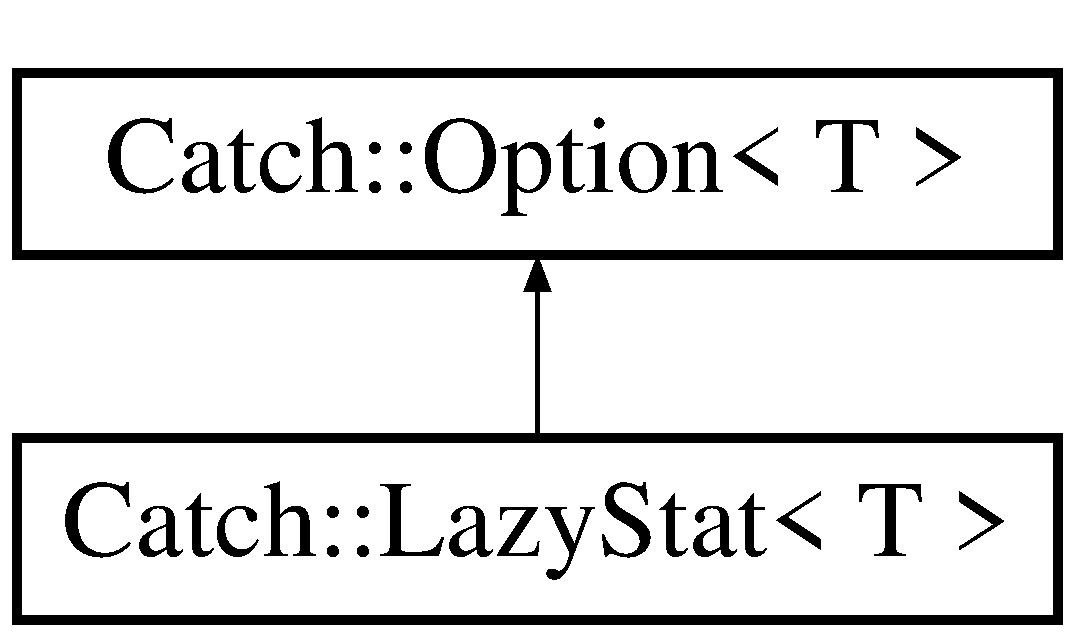
\includegraphics[height=2.000000cm]{class_catch_1_1_option}
\end{center}
\end{figure}
\subsection*{Public Member Functions}
\begin{DoxyCompactItemize}
\item 
\hypertarget{class_catch_1_1_option_a5aeb9c22d48a6882bdf5fb4730b06c86}{{\bfseries Option} (T const \&\-\_\-value)}\label{class_catch_1_1_option_a5aeb9c22d48a6882bdf5fb4730b06c86}

\item 
\hypertarget{class_catch_1_1_option_af02f2e4559f06384baec0def8c68c5fd}{{\bfseries Option} (\hyperlink{class_catch_1_1_option}{Option} const \&\-\_\-other)}\label{class_catch_1_1_option_af02f2e4559f06384baec0def8c68c5fd}

\item 
\hypertarget{class_catch_1_1_option_a78c65b15dd6b2fbd04c5012c43017c8f}{\hyperlink{class_catch_1_1_option}{Option} \& {\bfseries operator=} (\hyperlink{class_catch_1_1_option}{Option} const \&\-\_\-other)}\label{class_catch_1_1_option_a78c65b15dd6b2fbd04c5012c43017c8f}

\item 
\hypertarget{class_catch_1_1_option_a2be7e343ab22d6061726d32ab4622653}{\hyperlink{class_catch_1_1_option}{Option} \& {\bfseries operator=} (T const \&\-\_\-value)}\label{class_catch_1_1_option_a2be7e343ab22d6061726d32ab4622653}

\item 
\hypertarget{class_catch_1_1_option_a37b4e0e5d4d56296adacd267a616f4e0}{void {\bfseries reset} ()}\label{class_catch_1_1_option_a37b4e0e5d4d56296adacd267a616f4e0}

\item 
\hypertarget{class_catch_1_1_option_afd989852fa453731c3190dac63caccb0}{T \& {\bfseries operator$\ast$} ()}\label{class_catch_1_1_option_afd989852fa453731c3190dac63caccb0}

\item 
\hypertarget{class_catch_1_1_option_a0f05708905dc6b0b470fb24f5d265631}{T const \& {\bfseries operator$\ast$} () const }\label{class_catch_1_1_option_a0f05708905dc6b0b470fb24f5d265631}

\item 
\hypertarget{class_catch_1_1_option_acad340798a16c8f700f8763119e90f31}{T $\ast$ {\bfseries operator-\/$>$} ()}\label{class_catch_1_1_option_acad340798a16c8f700f8763119e90f31}

\item 
\hypertarget{class_catch_1_1_option_a0800340b2971748671b88acfb14bb928}{const T $\ast$ {\bfseries operator-\/$>$} () const }\label{class_catch_1_1_option_a0800340b2971748671b88acfb14bb928}

\item 
\hypertarget{class_catch_1_1_option_a21b5629a7febbe3e23c475c9d9138a2d}{T {\bfseries value\-Or} (T const \&default\-Value) const }\label{class_catch_1_1_option_a21b5629a7febbe3e23c475c9d9138a2d}

\item 
\hypertarget{class_catch_1_1_option_affa96f15798b4656fb753ff52d12dec2}{bool {\bfseries some} () const }\label{class_catch_1_1_option_affa96f15798b4656fb753ff52d12dec2}

\item 
\hypertarget{class_catch_1_1_option_a389324d2aa20ceb0eb0f48a5f77c20c8}{bool {\bfseries none} () const }\label{class_catch_1_1_option_a389324d2aa20ceb0eb0f48a5f77c20c8}

\item 
\hypertarget{class_catch_1_1_option_a47a1b6f6def2730ea9d27a1860a4f97f}{bool {\bfseries operator!} () const }\label{class_catch_1_1_option_a47a1b6f6def2730ea9d27a1860a4f97f}

\item 
\hypertarget{class_catch_1_1_option_a637d4366ae7f0ded52ce59c8cb06da7b}{{\bfseries operator Safe\-Bool\-::type} () const }\label{class_catch_1_1_option_a637d4366ae7f0ded52ce59c8cb06da7b}

\end{DoxyCompactItemize}


The documentation for this class was generated from the following file\-:\begin{DoxyCompactItemize}
\item 
Catch.\-h\end{DoxyCompactItemize}

\hypertarget{struct_catch_1_1_output_debug_writer}{\section{Catch\-:\-:Output\-Debug\-Writer Struct Reference}
\label{struct_catch_1_1_output_debug_writer}\index{Catch\-::\-Output\-Debug\-Writer@{Catch\-::\-Output\-Debug\-Writer}}
}
\subsection*{Public Member Functions}
\begin{DoxyCompactItemize}
\item 
\hypertarget{struct_catch_1_1_output_debug_writer_a6ed4872c2e7b9396dce5168039362c29}{void {\bfseries operator()} (std\-::string const \&str)}\label{struct_catch_1_1_output_debug_writer_a6ed4872c2e7b9396dce5168039362c29}

\end{DoxyCompactItemize}


The documentation for this struct was generated from the following file\-:\begin{DoxyCompactItemize}
\item 
Catch.\-h\end{DoxyCompactItemize}

\hypertarget{class_p_d_a}{\section{P\-D\-A Class Reference}
\label{class_p_d_a}\index{P\-D\-A@{P\-D\-A}}
}


Class representing a \hyperlink{class_p_d_a}{P\-D\-A}.  




{\ttfamily \#include $<$P\-D\-A.\-h$>$}

\subsection*{Public Member Functions}
\begin{DoxyCompactItemize}
\item 
\hyperlink{class_p_d_a_ada371103866d34235247f65ddbd5bf8e}{P\-D\-A} (const std\-::set$<$ char $>$ \&alphabet\-P\-D\-A, const std\-::set$<$ char $>$ \&alphabet\-Stack, const P\-D\-A\-Final \&P\-D\-Aending)
\begin{DoxyCompactList}\small\item\em Constructor. \end{DoxyCompactList}\item 
\hyperlink{class_p_d_a_a0bb4ed22f081c4b89510021fdf8aa125}{P\-D\-A} (\hyperlink{class_c_f_g}{C\-F\-G} cfg)
\begin{DoxyCompactList}\small\item\em Constructor. \end{DoxyCompactList}\item 
\hyperlink{class_p_d_a_a5bdc4c651e9b6da0b76cf61504c82034}{P\-D\-A} (const std\-::string \&file\-Name)
\begin{DoxyCompactList}\small\item\em Constructor. \end{DoxyCompactList}\item 
bool \hyperlink{class_p_d_a_a15e2bf53b9d534b9df4753772c480000}{add\-State} (const \hyperlink{class_p_d_a_state}{P\-D\-A\-State} \&state)
\begin{DoxyCompactList}\small\item\em Add a new state to the \hyperlink{class_p_d_a}{P\-D\-A}. \end{DoxyCompactList}\item 
bool \hyperlink{class_p_d_a_aed594ef143a2a18a685c262e99db66d4}{add\-State} (const \hyperlink{class_p_d_a_state}{P\-D\-A\-State} \&state, const bool \&is\-Starting)
\begin{DoxyCompactList}\small\item\em Add a new state to the \hyperlink{class_p_d_a}{P\-D\-A}. \end{DoxyCompactList}\item 
bool \hyperlink{class_p_d_a_af890a0efdc27538e4febe35d80dc9b61}{add\-Transition} (\hyperlink{class_p_d_a_transition}{P\-D\-A\-Transition} transition)
\begin{DoxyCompactList}\small\item\em Add a new transition to the \hyperlink{class_p_d_a}{P\-D\-A}. \end{DoxyCompactList}\item 
bool \hyperlink{class_p_d_a_a6ae74a864d002fcd9b1e1118b72ce1ab}{process} (std\-::string input)
\begin{DoxyCompactList}\small\item\em Process an input string through the \hyperlink{class_p_d_a}{P\-D\-A}. \end{DoxyCompactList}\end{DoxyCompactItemize}
\subsection*{Friends}
\begin{DoxyCompactItemize}
\item 
\hypertarget{class_p_d_a_aee90424d2ee8825402f2028e2cb5cbd8}{std\-::ostream \& \hyperlink{class_p_d_a_aee90424d2ee8825402f2028e2cb5cbd8}{operator$<$$<$} (std\-::ostream \&out, \hyperlink{class_p_d_a}{P\-D\-A} pda)}\label{class_p_d_a_aee90424d2ee8825402f2028e2cb5cbd8}

\begin{DoxyCompactList}\small\item\em $<$$<$ overloading \end{DoxyCompactList}\end{DoxyCompactItemize}


\subsection{Detailed Description}
Class representing a \hyperlink{class_p_d_a}{P\-D\-A}. 

\subsection{Constructor \& Destructor Documentation}
\hypertarget{class_p_d_a_ada371103866d34235247f65ddbd5bf8e}{\index{P\-D\-A@{P\-D\-A}!P\-D\-A@{P\-D\-A}}
\index{P\-D\-A@{P\-D\-A}!PDA@{P\-D\-A}}
\subsubsection[{P\-D\-A}]{\setlength{\rightskip}{0pt plus 5cm}P\-D\-A\-::\-P\-D\-A (
\begin{DoxyParamCaption}
\item[{const std\-::set$<$ char $>$ \&}]{alphabet\-P\-D\-A, }
\item[{const std\-::set$<$ char $>$ \&}]{alphabet\-Stack, }
\item[{const P\-D\-A\-Final \&}]{P\-D\-Aending}
\end{DoxyParamCaption}
)}}\label{class_p_d_a_ada371103866d34235247f65ddbd5bf8e}


Constructor. 


\begin{DoxyParams}{Parameters}
{\em alphabet\-P\-D\-A} & A set containing characters representing the alphabet of the \hyperlink{class_p_d_a}{P\-D\-A} \\
\hline
{\em alphabet\-Stack} & A set containing characters representing the alphabet of the stack \\
\hline
{\em P\-D\-Aending} & The type of P\-D\-A(\-S\-T\-A\-C\-K\-: P\-D\-A is final with empty stack, S\-T\-A\-T\-E\-: P\-D\-A is final when it reaches an empty state) \\
\hline
\end{DoxyParams}
\hypertarget{class_p_d_a_a0bb4ed22f081c4b89510021fdf8aa125}{\index{P\-D\-A@{P\-D\-A}!P\-D\-A@{P\-D\-A}}
\index{P\-D\-A@{P\-D\-A}!PDA@{P\-D\-A}}
\subsubsection[{P\-D\-A}]{\setlength{\rightskip}{0pt plus 5cm}P\-D\-A\-::\-P\-D\-A (
\begin{DoxyParamCaption}
\item[{{\bf C\-F\-G}}]{cfg}
\end{DoxyParamCaption}
)}}\label{class_p_d_a_a0bb4ed22f081c4b89510021fdf8aa125}


Constructor. 


\begin{DoxyParams}{Parameters}
{\em cfg} & A Context Free Grammar to be transformed to a \hyperlink{class_p_d_a}{P\-D\-A} \\
\hline
\end{DoxyParams}
\hypertarget{class_p_d_a_a5bdc4c651e9b6da0b76cf61504c82034}{\index{P\-D\-A@{P\-D\-A}!P\-D\-A@{P\-D\-A}}
\index{P\-D\-A@{P\-D\-A}!PDA@{P\-D\-A}}
\subsubsection[{P\-D\-A}]{\setlength{\rightskip}{0pt plus 5cm}P\-D\-A\-::\-P\-D\-A (
\begin{DoxyParamCaption}
\item[{const std\-::string \&}]{file\-Name}
\end{DoxyParamCaption}
)}}\label{class_p_d_a_a5bdc4c651e9b6da0b76cf61504c82034}


Constructor. 


\begin{DoxyParams}{Parameters}
{\em file\-Name} & A X\-M\-L file containing info about the \hyperlink{class_p_d_a}{P\-D\-A} \\
\hline
\end{DoxyParams}


\subsection{Member Function Documentation}
\hypertarget{class_p_d_a_a15e2bf53b9d534b9df4753772c480000}{\index{P\-D\-A@{P\-D\-A}!add\-State@{add\-State}}
\index{add\-State@{add\-State}!PDA@{P\-D\-A}}
\subsubsection[{add\-State}]{\setlength{\rightskip}{0pt plus 5cm}bool P\-D\-A\-::add\-State (
\begin{DoxyParamCaption}
\item[{const {\bf P\-D\-A\-State} \&}]{state}
\end{DoxyParamCaption}
)}}\label{class_p_d_a_a15e2bf53b9d534b9df4753772c480000}


Add a new state to the \hyperlink{class_p_d_a}{P\-D\-A}. 


\begin{DoxyParams}{Parameters}
{\em state} & An \hyperlink{class_p_d_a_state}{P\-D\-A\-State} object representing an \hyperlink{class_p_d_a}{P\-D\-A} state\\
\hline
\end{DoxyParams}
\begin{DoxyReturn}{Returns}
A bool telling if the state is added or not 
\end{DoxyReturn}
\hypertarget{class_p_d_a_aed594ef143a2a18a685c262e99db66d4}{\index{P\-D\-A@{P\-D\-A}!add\-State@{add\-State}}
\index{add\-State@{add\-State}!PDA@{P\-D\-A}}
\subsubsection[{add\-State}]{\setlength{\rightskip}{0pt plus 5cm}bool P\-D\-A\-::add\-State (
\begin{DoxyParamCaption}
\item[{const {\bf P\-D\-A\-State} \&}]{state, }
\item[{const bool \&}]{is\-Starting}
\end{DoxyParamCaption}
)}}\label{class_p_d_a_aed594ef143a2a18a685c262e99db66d4}


Add a new state to the \hyperlink{class_p_d_a}{P\-D\-A}. 


\begin{DoxyParams}{Parameters}
{\em state} & A \hyperlink{class_p_d_a_state}{P\-D\-A\-State} object representing an \hyperlink{class_p_d_a}{P\-D\-A} state \\
\hline
{\em is\-Starting} & A bool describing if the state is the start state\\
\hline
\end{DoxyParams}
\begin{DoxyReturn}{Returns}
A bool telling if the state is added or not 
\end{DoxyReturn}
\hypertarget{class_p_d_a_af890a0efdc27538e4febe35d80dc9b61}{\index{P\-D\-A@{P\-D\-A}!add\-Transition@{add\-Transition}}
\index{add\-Transition@{add\-Transition}!PDA@{P\-D\-A}}
\subsubsection[{add\-Transition}]{\setlength{\rightskip}{0pt plus 5cm}bool P\-D\-A\-::add\-Transition (
\begin{DoxyParamCaption}
\item[{{\bf P\-D\-A\-Transition}}]{transition}
\end{DoxyParamCaption}
)}}\label{class_p_d_a_af890a0efdc27538e4febe35d80dc9b61}


Add a new transition to the \hyperlink{class_p_d_a}{P\-D\-A}. 


\begin{DoxyParams}{Parameters}
{\em transition} & A \hyperlink{class_p_d_a_transition}{P\-D\-A\-Transition} object representing an \hyperlink{class_p_d_a}{P\-D\-A} transition\\
\hline
\end{DoxyParams}
\begin{DoxyReturn}{Returns}
A bool telling if the transition is added or not 
\end{DoxyReturn}
\hypertarget{class_p_d_a_a6ae74a864d002fcd9b1e1118b72ce1ab}{\index{P\-D\-A@{P\-D\-A}!process@{process}}
\index{process@{process}!PDA@{P\-D\-A}}
\subsubsection[{process}]{\setlength{\rightskip}{0pt plus 5cm}bool P\-D\-A\-::process (
\begin{DoxyParamCaption}
\item[{std\-::string}]{input}
\end{DoxyParamCaption}
)}}\label{class_p_d_a_a6ae74a864d002fcd9b1e1118b72ce1ab}


Process an input string through the \hyperlink{class_p_d_a}{P\-D\-A}. 


\begin{DoxyParams}{Parameters}
{\em input} & The string to be processed by the \hyperlink{class_p_d_a}{P\-D\-A}\\
\hline
\end{DoxyParams}
\begin{DoxyReturn}{Returns}
A bool telling if the \hyperlink{class_p_d_a}{P\-D\-A} ended in a final state or empty stack 
\end{DoxyReturn}


The documentation for this class was generated from the following files\-:\begin{DoxyCompactItemize}
\item 
P\-D\-A.\-h\item 
P\-D\-A.\-cpp\end{DoxyCompactItemize}

\hypertarget{class_p_d_a_i_d}{\section{P\-D\-A\-I\-D Class Reference}
\label{class_p_d_a_i_d}\index{P\-D\-A\-I\-D@{P\-D\-A\-I\-D}}
}


Class representing a \hyperlink{class_p_d_a}{P\-D\-A} Instantenious Description.  




{\ttfamily \#include $<$P\-D\-A.\-h$>$}

\subsection*{Public Member Functions}
\begin{DoxyCompactItemize}
\item 
\hyperlink{class_p_d_a_i_d_a2771c16218559b027029c12a0135353a}{P\-D\-A\-I\-D} (const std\-::string \&input, \hyperlink{class_p_d_a_state}{P\-D\-A\-State} $\ast$current\-State, const std\-::stack$<$ char $>$ stack)
\begin{DoxyCompactList}\small\item\em Constructor. \end{DoxyCompactList}\item 
void \hyperlink{class_p_d_a_i_d_aa5ffd9bde5a3a86648ffedfd3932070b}{step} (const std\-::string \&input, \hyperlink{class_p_d_a_state}{P\-D\-A\-State} $\ast$current\-State, const std\-::stack$<$ char $>$ stack)
\begin{DoxyCompactList}\small\item\em Process the I\-D according to one transition for one step. \end{DoxyCompactList}\item 
bool \hyperlink{class_p_d_a_i_d_a85f6765dd9c0244f07dc44822c223d46}{is\-Accepted} (P\-D\-A\-Final pda\-Type)
\begin{DoxyCompactList}\small\item\em Check if this I\-D will be accepted by the \hyperlink{class_p_d_a}{P\-D\-A}. \end{DoxyCompactList}\item 
\hypertarget{class_p_d_a_i_d_a55955e1bb7212989f671863f2f628f79}{std\-::string {\bfseries get\-Input} ()}\label{class_p_d_a_i_d_a55955e1bb7212989f671863f2f628f79}

\item 
\hypertarget{class_p_d_a_i_d_a87dbd8ad4bec917fbf17959e87b74884}{\hyperlink{class_p_d_a_state}{P\-D\-A\-State} $\ast$ {\bfseries get\-State} ()}\label{class_p_d_a_i_d_a87dbd8ad4bec917fbf17959e87b74884}

\item 
\hypertarget{class_p_d_a_i_d_acde6beb96c3f71a8f2e287828a7ab66d}{std\-::stack$<$ char $>$ {\bfseries get\-Stack} ()}\label{class_p_d_a_i_d_acde6beb96c3f71a8f2e287828a7ab66d}

\end{DoxyCompactItemize}
\subsection*{Friends}
\begin{DoxyCompactItemize}
\item 
\hypertarget{class_p_d_a_i_d_a0747801e76043464e9ed4f9e8b749e27}{std\-::ostream \& \hyperlink{class_p_d_a_i_d_a0747801e76043464e9ed4f9e8b749e27}{operator$<$$<$} (std\-::ostream \&out, \hyperlink{class_p_d_a_i_d}{P\-D\-A\-I\-D} id)}\label{class_p_d_a_i_d_a0747801e76043464e9ed4f9e8b749e27}

\begin{DoxyCompactList}\small\item\em $<$$<$ overloading \end{DoxyCompactList}\end{DoxyCompactItemize}


\subsection{Detailed Description}
Class representing a \hyperlink{class_p_d_a}{P\-D\-A} Instantenious Description. 

\subsection{Constructor \& Destructor Documentation}
\hypertarget{class_p_d_a_i_d_a2771c16218559b027029c12a0135353a}{\index{P\-D\-A\-I\-D@{P\-D\-A\-I\-D}!P\-D\-A\-I\-D@{P\-D\-A\-I\-D}}
\index{P\-D\-A\-I\-D@{P\-D\-A\-I\-D}!PDAID@{P\-D\-A\-I\-D}}
\subsubsection[{P\-D\-A\-I\-D}]{\setlength{\rightskip}{0pt plus 5cm}P\-D\-A\-I\-D\-::\-P\-D\-A\-I\-D (
\begin{DoxyParamCaption}
\item[{const std\-::string \&}]{input, }
\item[{{\bf P\-D\-A\-State} $\ast$}]{current\-State, }
\item[{const std\-::stack$<$ char $>$}]{stack}
\end{DoxyParamCaption}
)}}\label{class_p_d_a_i_d_a2771c16218559b027029c12a0135353a}


Constructor. 


\begin{DoxyParams}{Parameters}
{\em input} & The input string \\
\hline
{\em current\-State} & The pointer to state where the I\-D starts \\
\hline
{\em stack} & The stack at this moment \\
\hline
\end{DoxyParams}


\subsection{Member Function Documentation}
\hypertarget{class_p_d_a_i_d_a85f6765dd9c0244f07dc44822c223d46}{\index{P\-D\-A\-I\-D@{P\-D\-A\-I\-D}!is\-Accepted@{is\-Accepted}}
\index{is\-Accepted@{is\-Accepted}!PDAID@{P\-D\-A\-I\-D}}
\subsubsection[{is\-Accepted}]{\setlength{\rightskip}{0pt plus 5cm}bool P\-D\-A\-I\-D\-::is\-Accepted (
\begin{DoxyParamCaption}
\item[{P\-D\-A\-Final}]{pda\-Type}
\end{DoxyParamCaption}
)}}\label{class_p_d_a_i_d_a85f6765dd9c0244f07dc44822c223d46}


Check if this I\-D will be accepted by the \hyperlink{class_p_d_a}{P\-D\-A}. 


\begin{DoxyParams}{Parameters}
{\em pda\-Type} & Type of P\-D\-A(\-State or Stack)\\
\hline
\end{DoxyParams}
\begin{DoxyReturn}{Returns}
bool telling if the I\-D is accepted 
\end{DoxyReturn}
\hypertarget{class_p_d_a_i_d_aa5ffd9bde5a3a86648ffedfd3932070b}{\index{P\-D\-A\-I\-D@{P\-D\-A\-I\-D}!step@{step}}
\index{step@{step}!PDAID@{P\-D\-A\-I\-D}}
\subsubsection[{step}]{\setlength{\rightskip}{0pt plus 5cm}void P\-D\-A\-I\-D\-::step (
\begin{DoxyParamCaption}
\item[{const std\-::string \&}]{input, }
\item[{{\bf P\-D\-A\-State} $\ast$}]{current\-State, }
\item[{const std\-::stack$<$ char $>$}]{stack}
\end{DoxyParamCaption}
)}}\label{class_p_d_a_i_d_aa5ffd9bde5a3a86648ffedfd3932070b}


Process the I\-D according to one transition for one step. 


\begin{DoxyParams}{Parameters}
{\em to} & Pointer to next state \\
\hline
{\em input\-Symbol} & Character accompanied with this transition \\
\hline
{\em top\-Stack} & Character that should be at the top of the stack after the transition \\
\hline
\end{DoxyParams}


The documentation for this class was generated from the following files\-:\begin{DoxyCompactItemize}
\item 
P\-D\-A.\-h\item 
P\-D\-A.\-cpp\end{DoxyCompactItemize}

\hypertarget{class_p_d_a_state}{\section{P\-D\-A\-State Class Reference}
\label{class_p_d_a_state}\index{P\-D\-A\-State@{P\-D\-A\-State}}
}


Class representing a state from a \hyperlink{class_p_d_a}{P\-D\-A}.  




{\ttfamily \#include $<$P\-D\-A.\-h$>$}

\subsection*{Public Member Functions}
\begin{DoxyCompactItemize}
\item 
\hyperlink{class_p_d_a_state_a23a8145588cdb3d637009cde2772b231}{P\-D\-A\-State} (std\-::string name)
\begin{DoxyCompactList}\small\item\em Constructor. \end{DoxyCompactList}\item 
\hyperlink{class_p_d_a_state_a22f60087f927a3f6eec2d32d399a3a59}{P\-D\-A\-State} (std\-::string name, bool \hyperlink{class_p_d_a_state_a2d0b019768390195609cb86c774012e3}{is\-Final})
\begin{DoxyCompactList}\small\item\em Constructor. \end{DoxyCompactList}\item 
bool \hyperlink{class_p_d_a_state_a2d0b019768390195609cb86c774012e3}{is\-Final} () const 
\begin{DoxyCompactList}\small\item\em Check if a state is final. \end{DoxyCompactList}\item 
std\-::string \hyperlink{class_p_d_a_state_adc47d2550f6febc18e67a19e951063ce}{get\-Name} () const 
\begin{DoxyCompactList}\small\item\em Get the name of the state. \end{DoxyCompactList}\item 
bool \hyperlink{class_p_d_a_state_a4f82e8ecf6c1cff3c255c647302a43b5}{operator==} (const \hyperlink{class_p_d_a_state}{P\-D\-A\-State} \&other)
\begin{DoxyCompactList}\small\item\em == operator overloading \end{DoxyCompactList}\end{DoxyCompactItemize}
\subsection*{Friends}
\begin{DoxyCompactItemize}
\item 
\hypertarget{class_p_d_a_state_af3c8e5862ec2b5e19c42d81317103097}{std\-::ostream \& \hyperlink{class_p_d_a_state_af3c8e5862ec2b5e19c42d81317103097}{operator$<$$<$} (std\-::ostream \&out, \hyperlink{class_p_d_a_state}{P\-D\-A\-State} state)}\label{class_p_d_a_state_af3c8e5862ec2b5e19c42d81317103097}

\begin{DoxyCompactList}\small\item\em $<$$<$ overloading \end{DoxyCompactList}\end{DoxyCompactItemize}


\subsection{Detailed Description}
Class representing a state from a \hyperlink{class_p_d_a}{P\-D\-A}. 

\subsection{Constructor \& Destructor Documentation}
\hypertarget{class_p_d_a_state_a23a8145588cdb3d637009cde2772b231}{\index{P\-D\-A\-State@{P\-D\-A\-State}!P\-D\-A\-State@{P\-D\-A\-State}}
\index{P\-D\-A\-State@{P\-D\-A\-State}!PDAState@{P\-D\-A\-State}}
\subsubsection[{P\-D\-A\-State}]{\setlength{\rightskip}{0pt plus 5cm}P\-D\-A\-State\-::\-P\-D\-A\-State (
\begin{DoxyParamCaption}
\item[{std\-::string}]{name}
\end{DoxyParamCaption}
)}}\label{class_p_d_a_state_a23a8145588cdb3d637009cde2772b231}


Constructor. 


\begin{DoxyParams}{Parameters}
{\em name} & The name of the \hyperlink{class_p_d_a_state}{P\-D\-A\-State} \\
\hline
\end{DoxyParams}
\hypertarget{class_p_d_a_state_a22f60087f927a3f6eec2d32d399a3a59}{\index{P\-D\-A\-State@{P\-D\-A\-State}!P\-D\-A\-State@{P\-D\-A\-State}}
\index{P\-D\-A\-State@{P\-D\-A\-State}!PDAState@{P\-D\-A\-State}}
\subsubsection[{P\-D\-A\-State}]{\setlength{\rightskip}{0pt plus 5cm}P\-D\-A\-State\-::\-P\-D\-A\-State (
\begin{DoxyParamCaption}
\item[{std\-::string}]{name, }
\item[{bool}]{is\-Final}
\end{DoxyParamCaption}
)}}\label{class_p_d_a_state_a22f60087f927a3f6eec2d32d399a3a59}


Constructor. 


\begin{DoxyParams}{Parameters}
{\em name} & The name of the \hyperlink{class_p_d_a_state}{P\-D\-A\-State} \\
\hline
{\em is\-Final} & Bool which tells if this state is final or not \\
\hline
\end{DoxyParams}


\subsection{Member Function Documentation}
\hypertarget{class_p_d_a_state_adc47d2550f6febc18e67a19e951063ce}{\index{P\-D\-A\-State@{P\-D\-A\-State}!get\-Name@{get\-Name}}
\index{get\-Name@{get\-Name}!PDAState@{P\-D\-A\-State}}
\subsubsection[{get\-Name}]{\setlength{\rightskip}{0pt plus 5cm}std\-::string P\-D\-A\-State\-::get\-Name (
\begin{DoxyParamCaption}
{}
\end{DoxyParamCaption}
) const}}\label{class_p_d_a_state_adc47d2550f6febc18e67a19e951063ce}


Get the name of the state. 

\begin{DoxyReturn}{Returns}
A string representing the name 
\end{DoxyReturn}
\hypertarget{class_p_d_a_state_a2d0b019768390195609cb86c774012e3}{\index{P\-D\-A\-State@{P\-D\-A\-State}!is\-Final@{is\-Final}}
\index{is\-Final@{is\-Final}!PDAState@{P\-D\-A\-State}}
\subsubsection[{is\-Final}]{\setlength{\rightskip}{0pt plus 5cm}bool P\-D\-A\-State\-::is\-Final (
\begin{DoxyParamCaption}
{}
\end{DoxyParamCaption}
) const}}\label{class_p_d_a_state_a2d0b019768390195609cb86c774012e3}


Check if a state is final. 

\begin{DoxyReturn}{Returns}
A bool telling if it's true or not 
\end{DoxyReturn}
\hypertarget{class_p_d_a_state_a4f82e8ecf6c1cff3c255c647302a43b5}{\index{P\-D\-A\-State@{P\-D\-A\-State}!operator==@{operator==}}
\index{operator==@{operator==}!PDAState@{P\-D\-A\-State}}
\subsubsection[{operator==}]{\setlength{\rightskip}{0pt plus 5cm}bool P\-D\-A\-State\-::operator== (
\begin{DoxyParamCaption}
\item[{const {\bf P\-D\-A\-State} \&}]{other}
\end{DoxyParamCaption}
)}}\label{class_p_d_a_state_a4f82e8ecf6c1cff3c255c647302a43b5}


== operator overloading 

\begin{DoxyReturn}{Returns}
Bool telling if the two states are equal 
\end{DoxyReturn}


The documentation for this class was generated from the following files\-:\begin{DoxyCompactItemize}
\item 
P\-D\-A.\-h\item 
P\-D\-A.\-cpp\end{DoxyCompactItemize}

\hypertarget{class_p_d_a_transition}{\section{P\-D\-A\-Transition Class Reference}
\label{class_p_d_a_transition}\index{P\-D\-A\-Transition@{P\-D\-A\-Transition}}
}


Class representing a transition from a \hyperlink{class_p_d_a}{P\-D\-A}.  




{\ttfamily \#include $<$P\-D\-A.\-h$>$}

\subsection*{Public Member Functions}
\begin{DoxyCompactItemize}
\item 
\hyperlink{class_p_d_a_transition_abbfb0059d8f657ad434e5b07d337e361}{P\-D\-A\-Transition} (\hyperlink{class_p_d_a_state}{P\-D\-A\-State} $\ast$from, \hyperlink{class_p_d_a_state}{P\-D\-A\-State} $\ast$to, const char \&input, const char \&stack\-Top, const P\-D\-A\-Stack\-Operation \&\hyperlink{class_p_d_a_transition_a66c5e45c981d66e326aac04749f5effa}{stack\-Operation})
\begin{DoxyCompactList}\small\item\em Constructor. \end{DoxyCompactList}\item 
\hyperlink{class_p_d_a_transition_a060bbd689533147e128fb7c4827fd801}{P\-D\-A\-Transition} (\hyperlink{class_p_d_a_state}{P\-D\-A\-State} $\ast$from, \hyperlink{class_p_d_a_state}{P\-D\-A\-State} $\ast$to, const char \&input, const char \&stack\-Top, const P\-D\-A\-Stack\-Operation \&\hyperlink{class_p_d_a_transition_a66c5e45c981d66e326aac04749f5effa}{stack\-Operation}, const char \&stack\-Push)
\begin{DoxyCompactList}\small\item\em Constructor. \end{DoxyCompactList}\item 
\hyperlink{class_p_d_a_transition_adf9edc281ee9ad54b07aea48ce85670e}{P\-D\-A\-Transition} (\hyperlink{class_p_d_a_state}{P\-D\-A\-State} $\ast$from, \hyperlink{class_p_d_a_state}{P\-D\-A\-State} $\ast$to, const char \&input, const char \&stack\-Top, const P\-D\-A\-Stack\-Operation \&\hyperlink{class_p_d_a_transition_a66c5e45c981d66e326aac04749f5effa}{stack\-Operation}, const std\-::vector$<$ char $>$ \&stack\-Push)
\begin{DoxyCompactList}\small\item\em Constructor. \end{DoxyCompactList}\item 
bool \hyperlink{class_p_d_a_transition_a56a59630ec8488b38d4a3995ff00b630}{operator==} (const \hyperlink{class_p_d_a_transition}{P\-D\-A\-Transition} \&other)
\begin{DoxyCompactList}\small\item\em == operator overloading \end{DoxyCompactList}\item 
void \hyperlink{class_p_d_a_transition_a66c5e45c981d66e326aac04749f5effa}{stack\-Operation} (std\-::stack$<$ char $>$ \&in)
\begin{DoxyCompactList}\small\item\em Change a stack based upon the data in the transition. \end{DoxyCompactList}\item 
\hypertarget{class_p_d_a_transition_ac4d9fb44b76fa8d22a7f1e64f8d416aa}{\hyperlink{class_p_d_a_state}{P\-D\-A\-State} $\ast$ {\bfseries get\-From} ()}\label{class_p_d_a_transition_ac4d9fb44b76fa8d22a7f1e64f8d416aa}

\item 
\hypertarget{class_p_d_a_transition_a8efc3ccc02e251f598a42a12013ec20e}{\hyperlink{class_p_d_a_state}{P\-D\-A\-State} $\ast$ {\bfseries get\-To} ()}\label{class_p_d_a_transition_a8efc3ccc02e251f598a42a12013ec20e}

\item 
\hypertarget{class_p_d_a_transition_a95e8f23dc7feb80284f9dc4eb9e5d679}{char {\bfseries get\-Input\-Symbol} ()}\label{class_p_d_a_transition_a95e8f23dc7feb80284f9dc4eb9e5d679}

\item 
\hypertarget{class_p_d_a_transition_a365f5d1060c7bc1d9def3605714a163f}{char {\bfseries get\-Top\-Stack} ()}\label{class_p_d_a_transition_a365f5d1060c7bc1d9def3605714a163f}

\item 
\hypertarget{class_p_d_a_transition_ac80fa0610beaf908fd847c7675425c2c}{P\-D\-A\-Stack\-Operation {\bfseries get\-Stack\-Operation} ()}\label{class_p_d_a_transition_ac80fa0610beaf908fd847c7675425c2c}

\item 
\hypertarget{class_p_d_a_transition_a7d7a667339612031202e596854c55754}{std\-::vector$<$ char $>$ {\bfseries get\-Push\-Stack} ()}\label{class_p_d_a_transition_a7d7a667339612031202e596854c55754}

\item 
\hypertarget{class_p_d_a_transition_ac157ed1fcb7d49979f627609faa2692a}{void {\bfseries set\-From} (\hyperlink{class_p_d_a_state}{P\-D\-A\-State} $\ast$from)}\label{class_p_d_a_transition_ac157ed1fcb7d49979f627609faa2692a}

\item 
\hypertarget{class_p_d_a_transition_a428abdc4df0c14ee945175b6733a4260}{void {\bfseries set\-To} (\hyperlink{class_p_d_a_state}{P\-D\-A\-State} $\ast$to)}\label{class_p_d_a_transition_a428abdc4df0c14ee945175b6733a4260}

\end{DoxyCompactItemize}
\subsection*{Friends}
\begin{DoxyCompactItemize}
\item 
\hypertarget{class_p_d_a_transition_aeb11e3ae2bf4258740c79bdcbc7f93b6}{std\-::ostream \& \hyperlink{class_p_d_a_transition_aeb11e3ae2bf4258740c79bdcbc7f93b6}{operator$<$$<$} (std\-::ostream \&out, \hyperlink{class_p_d_a_transition}{P\-D\-A\-Transition} transition)}\label{class_p_d_a_transition_aeb11e3ae2bf4258740c79bdcbc7f93b6}

\begin{DoxyCompactList}\small\item\em $<$$<$ overloading \end{DoxyCompactList}\end{DoxyCompactItemize}


\subsection{Detailed Description}
Class representing a transition from a \hyperlink{class_p_d_a}{P\-D\-A}. 

\subsection{Constructor \& Destructor Documentation}
\hypertarget{class_p_d_a_transition_abbfb0059d8f657ad434e5b07d337e361}{\index{P\-D\-A\-Transition@{P\-D\-A\-Transition}!P\-D\-A\-Transition@{P\-D\-A\-Transition}}
\index{P\-D\-A\-Transition@{P\-D\-A\-Transition}!PDATransition@{P\-D\-A\-Transition}}
\subsubsection[{P\-D\-A\-Transition}]{\setlength{\rightskip}{0pt plus 5cm}P\-D\-A\-Transition\-::\-P\-D\-A\-Transition (
\begin{DoxyParamCaption}
\item[{{\bf P\-D\-A\-State} $\ast$}]{from, }
\item[{{\bf P\-D\-A\-State} $\ast$}]{to, }
\item[{const char \&}]{input, }
\item[{const char \&}]{stack\-Top, }
\item[{const P\-D\-A\-Stack\-Operation \&}]{stack\-Operation}
\end{DoxyParamCaption}
)}}\label{class_p_d_a_transition_abbfb0059d8f657ad434e5b07d337e361}


Constructor. 


\begin{DoxyParams}{Parameters}
{\em from} & A pointer to the \hyperlink{class_p_d_a_state}{P\-D\-A\-State} where this transition is coming from \\
\hline
{\em to} & A pointer to the \hyperlink{class_p_d_a_state}{P\-D\-A\-State} where this transition is going to \\
\hline
{\em input} & The input symbol for the transition \\
\hline
{\em stack\-Top} & Define what should be on the top of the stack when processing this transition \\
\hline
{\em stack\-Operation} & Should the stack be popped, pushed or stay as it is \\
\hline
\end{DoxyParams}
\hypertarget{class_p_d_a_transition_a060bbd689533147e128fb7c4827fd801}{\index{P\-D\-A\-Transition@{P\-D\-A\-Transition}!P\-D\-A\-Transition@{P\-D\-A\-Transition}}
\index{P\-D\-A\-Transition@{P\-D\-A\-Transition}!PDATransition@{P\-D\-A\-Transition}}
\subsubsection[{P\-D\-A\-Transition}]{\setlength{\rightskip}{0pt plus 5cm}P\-D\-A\-Transition\-::\-P\-D\-A\-Transition (
\begin{DoxyParamCaption}
\item[{{\bf P\-D\-A\-State} $\ast$}]{from, }
\item[{{\bf P\-D\-A\-State} $\ast$}]{to, }
\item[{const char \&}]{input, }
\item[{const char \&}]{stack\-Top, }
\item[{const P\-D\-A\-Stack\-Operation \&}]{stack\-Operation, }
\item[{const char \&}]{stack\-Push}
\end{DoxyParamCaption}
)}}\label{class_p_d_a_transition_a060bbd689533147e128fb7c4827fd801}


Constructor. 


\begin{DoxyParams}{Parameters}
{\em from} & A pointer to the \hyperlink{class_p_d_a_state}{P\-D\-A\-State} where this transition is coming from \\
\hline
{\em to} & A pointer to the \hyperlink{class_p_d_a_state}{P\-D\-A\-State} where this transition is going to \\
\hline
{\em input} & The input symbol for the transition \\
\hline
{\em stack\-Top} & Define what should be on the top of the stack when processing this transition \\
\hline
{\em stack\-Operation} & Should the stack be popped, pushed or stay as it is \\
\hline
{\em stack\-Push} & The character that should be pushed to the stack during the transition \\
\hline
\end{DoxyParams}
\hypertarget{class_p_d_a_transition_adf9edc281ee9ad54b07aea48ce85670e}{\index{P\-D\-A\-Transition@{P\-D\-A\-Transition}!P\-D\-A\-Transition@{P\-D\-A\-Transition}}
\index{P\-D\-A\-Transition@{P\-D\-A\-Transition}!PDATransition@{P\-D\-A\-Transition}}
\subsubsection[{P\-D\-A\-Transition}]{\setlength{\rightskip}{0pt plus 5cm}P\-D\-A\-Transition\-::\-P\-D\-A\-Transition (
\begin{DoxyParamCaption}
\item[{{\bf P\-D\-A\-State} $\ast$}]{from, }
\item[{{\bf P\-D\-A\-State} $\ast$}]{to, }
\item[{const char \&}]{input, }
\item[{const char \&}]{stack\-Top, }
\item[{const P\-D\-A\-Stack\-Operation \&}]{stack\-Operation, }
\item[{const std\-::vector$<$ char $>$ \&}]{stack\-Push}
\end{DoxyParamCaption}
)}}\label{class_p_d_a_transition_adf9edc281ee9ad54b07aea48ce85670e}


Constructor. 


\begin{DoxyParams}{Parameters}
{\em from} & A pointer to the \hyperlink{class_p_d_a_state}{P\-D\-A\-State} where this transition is coming from \\
\hline
{\em to} & A pointer to the \hyperlink{class_p_d_a_state}{P\-D\-A\-State} where this transition is going to \\
\hline
{\em input} & The input symbol for the transition \\
\hline
{\em stack\-Top} & Define what should be on the top of the stack when processing this transition \\
\hline
{\em stack\-Operation} & Should the stack be popped, pushed or stay as it is \\
\hline
{\em stack\-Push} & The character vector that should be pushed to the stack during the transition \\
\hline
\end{DoxyParams}


\subsection{Member Function Documentation}
\hypertarget{class_p_d_a_transition_a56a59630ec8488b38d4a3995ff00b630}{\index{P\-D\-A\-Transition@{P\-D\-A\-Transition}!operator==@{operator==}}
\index{operator==@{operator==}!PDATransition@{P\-D\-A\-Transition}}
\subsubsection[{operator==}]{\setlength{\rightskip}{0pt plus 5cm}bool P\-D\-A\-Transition\-::operator== (
\begin{DoxyParamCaption}
\item[{const {\bf P\-D\-A\-Transition} \&}]{other}
\end{DoxyParamCaption}
)}}\label{class_p_d_a_transition_a56a59630ec8488b38d4a3995ff00b630}


== operator overloading 

\begin{DoxyReturn}{Returns}
Bool telling if the two transitions are equal 
\end{DoxyReturn}
\hypertarget{class_p_d_a_transition_a66c5e45c981d66e326aac04749f5effa}{\index{P\-D\-A\-Transition@{P\-D\-A\-Transition}!stack\-Operation@{stack\-Operation}}
\index{stack\-Operation@{stack\-Operation}!PDATransition@{P\-D\-A\-Transition}}
\subsubsection[{stack\-Operation}]{\setlength{\rightskip}{0pt plus 5cm}void P\-D\-A\-Transition\-::stack\-Operation (
\begin{DoxyParamCaption}
\item[{std\-::stack$<$ char $>$ \&}]{in}
\end{DoxyParamCaption}
)}}\label{class_p_d_a_transition_a66c5e45c981d66e326aac04749f5effa}


Change a stack based upon the data in the transition. 


\begin{DoxyParams}{Parameters}
{\em in} & A stack with chars representing the stack in the \hyperlink{class_p_d_a}{P\-D\-A}. Be careful! The stack is given by reference \\
\hline
\end{DoxyParams}


The documentation for this class was generated from the following files\-:\begin{DoxyCompactItemize}
\item 
P\-D\-A.\-h\item 
P\-D\-A.\-cpp\end{DoxyCompactItemize}

\hypertarget{struct_catch_1_1pluralise}{\section{Catch\-:\-:pluralise Struct Reference}
\label{struct_catch_1_1pluralise}\index{Catch\-::pluralise@{Catch\-::pluralise}}
}
\subsection*{Public Member Functions}
\begin{DoxyCompactItemize}
\item 
\hypertarget{struct_catch_1_1pluralise_a5c55e22de2416cfe416edf715c6b9234}{{\bfseries pluralise} (std\-::size\-\_\-t count, std\-::string const \&label)}\label{struct_catch_1_1pluralise_a5c55e22de2416cfe416edf715c6b9234}

\end{DoxyCompactItemize}
\subsection*{Public Attributes}
\begin{DoxyCompactItemize}
\item 
\hypertarget{struct_catch_1_1pluralise_a4dce2fa13ec6f00fac09b2418265441e}{std\-::size\-\_\-t {\bfseries m\-\_\-count}}\label{struct_catch_1_1pluralise_a4dce2fa13ec6f00fac09b2418265441e}

\item 
\hypertarget{struct_catch_1_1pluralise_a8849cbdd3f11ebe7747597c8644e8793}{std\-::string {\bfseries m\-\_\-label}}\label{struct_catch_1_1pluralise_a8849cbdd3f11ebe7747597c8644e8793}

\end{DoxyCompactItemize}
\subsection*{Friends}
\begin{DoxyCompactItemize}
\item 
\hypertarget{struct_catch_1_1pluralise_aa7dac6b165514c1f85e0695d678fdef5}{std\-::ostream \& {\bfseries operator$<$$<$} (std\-::ostream \&os, \hyperlink{struct_catch_1_1pluralise}{pluralise} const \&pluraliser)}\label{struct_catch_1_1pluralise_aa7dac6b165514c1f85e0695d678fdef5}

\end{DoxyCompactItemize}


The documentation for this struct was generated from the following file\-:\begin{DoxyCompactItemize}
\item 
Catch.\-h\end{DoxyCompactItemize}

\hypertarget{class_catch_1_1_ptr}{\section{Catch\-:\-:Ptr$<$ T $>$ Class Template Reference}
\label{class_catch_1_1_ptr}\index{Catch\-::\-Ptr$<$ T $>$@{Catch\-::\-Ptr$<$ T $>$}}
}
\subsection*{Public Member Functions}
\begin{DoxyCompactItemize}
\item 
\hypertarget{class_catch_1_1_ptr_aacec063a79cd142e39040a31c6b3c40b}{{\bfseries Ptr} (T $\ast$p)}\label{class_catch_1_1_ptr_aacec063a79cd142e39040a31c6b3c40b}

\item 
\hypertarget{class_catch_1_1_ptr_ac629dd8ebe5763a37bb89e6c1d6a1771}{{\bfseries Ptr} (\hyperlink{class_catch_1_1_ptr}{Ptr} const \&other)}\label{class_catch_1_1_ptr_ac629dd8ebe5763a37bb89e6c1d6a1771}

\item 
\hypertarget{class_catch_1_1_ptr_af8d0fa7a2cd20842830b354ac31dfe5c}{void {\bfseries reset} ()}\label{class_catch_1_1_ptr_af8d0fa7a2cd20842830b354ac31dfe5c}

\item 
\hypertarget{class_catch_1_1_ptr_a9b08c868b447d679ed201921f5c94683}{\hyperlink{class_catch_1_1_ptr}{Ptr} \& {\bfseries operator=} (T $\ast$p)}\label{class_catch_1_1_ptr_a9b08c868b447d679ed201921f5c94683}

\item 
\hypertarget{class_catch_1_1_ptr_af42074444c1bc6a70ebdc406a8617708}{\hyperlink{class_catch_1_1_ptr}{Ptr} \& {\bfseries operator=} (\hyperlink{class_catch_1_1_ptr}{Ptr} const \&other)}\label{class_catch_1_1_ptr_af42074444c1bc6a70ebdc406a8617708}

\item 
\hypertarget{class_catch_1_1_ptr_a172bf8b4e71e26a5a4d92f5b02158b50}{void {\bfseries swap} (\hyperlink{class_catch_1_1_ptr}{Ptr} \&other)}\label{class_catch_1_1_ptr_a172bf8b4e71e26a5a4d92f5b02158b50}

\item 
\hypertarget{class_catch_1_1_ptr_a0123036c2fca74afceea9c0e3e5cc01b}{T $\ast$ {\bfseries get} ()}\label{class_catch_1_1_ptr_a0123036c2fca74afceea9c0e3e5cc01b}

\item 
\hypertarget{class_catch_1_1_ptr_abf6f4d2d554086d9a2606add07716a16}{const T $\ast$ {\bfseries get} () const }\label{class_catch_1_1_ptr_abf6f4d2d554086d9a2606add07716a16}

\item 
\hypertarget{class_catch_1_1_ptr_a3a4c139032a8bd1bffa553103d5dbfd3}{T \& {\bfseries operator$\ast$} () const }\label{class_catch_1_1_ptr_a3a4c139032a8bd1bffa553103d5dbfd3}

\item 
\hypertarget{class_catch_1_1_ptr_afaa13250d5e0ae5a440726d5e5aa7295}{T $\ast$ {\bfseries operator-\/$>$} () const }\label{class_catch_1_1_ptr_afaa13250d5e0ae5a440726d5e5aa7295}

\item 
\hypertarget{class_catch_1_1_ptr_aea1a99ded6d62423ccb9173fab91b56e}{bool {\bfseries operator!} () const }\label{class_catch_1_1_ptr_aea1a99ded6d62423ccb9173fab91b56e}

\item 
\hypertarget{class_catch_1_1_ptr_a27234c04feec43ffe0fd08e045557448}{{\bfseries operator Safe\-Bool\-::type} () const }\label{class_catch_1_1_ptr_a27234c04feec43ffe0fd08e045557448}

\end{DoxyCompactItemize}


The documentation for this class was generated from the following file\-:\begin{DoxyCompactItemize}
\item 
Catch.\-h\end{DoxyCompactItemize}

\hypertarget{struct_catch_1_1_reporter_config}{\section{Catch\-:\-:Reporter\-Config Struct Reference}
\label{struct_catch_1_1_reporter_config}\index{Catch\-::\-Reporter\-Config@{Catch\-::\-Reporter\-Config}}
}
\subsection*{Public Member Functions}
\begin{DoxyCompactItemize}
\item 
\hypertarget{struct_catch_1_1_reporter_config_aae30a67f41d2b2fecd57f42f54649caa}{{\bfseries Reporter\-Config} (\hyperlink{class_catch_1_1_ptr}{Ptr}$<$ \hyperlink{struct_catch_1_1_i_config}{I\-Config} $>$ const \&\-\_\-full\-Config)}\label{struct_catch_1_1_reporter_config_aae30a67f41d2b2fecd57f42f54649caa}

\item 
\hypertarget{struct_catch_1_1_reporter_config_aadf290549fd003a753b938d824e75667}{{\bfseries Reporter\-Config} (\hyperlink{class_catch_1_1_ptr}{Ptr}$<$ \hyperlink{struct_catch_1_1_i_config}{I\-Config} $>$ const \&\-\_\-full\-Config, std\-::ostream \&\-\_\-stream)}\label{struct_catch_1_1_reporter_config_aadf290549fd003a753b938d824e75667}

\item 
\hypertarget{struct_catch_1_1_reporter_config_a6ac1cce9cdc14d4df5d3cea096c0910e}{std\-::ostream \& {\bfseries stream} () const }\label{struct_catch_1_1_reporter_config_a6ac1cce9cdc14d4df5d3cea096c0910e}

\item 
\hypertarget{struct_catch_1_1_reporter_config_a1d12c4a0a6c0c5619a3c8a12cf6fbf1d}{\hyperlink{class_catch_1_1_ptr}{Ptr}$<$ \hyperlink{struct_catch_1_1_i_config}{I\-Config} $>$ {\bfseries full\-Config} () const }\label{struct_catch_1_1_reporter_config_a1d12c4a0a6c0c5619a3c8a12cf6fbf1d}

\end{DoxyCompactItemize}


The documentation for this struct was generated from the following file\-:\begin{DoxyCompactItemize}
\item 
Catch.\-h\end{DoxyCompactItemize}

\hypertarget{struct_catch_1_1_reporter_preferences}{\section{Catch\-:\-:Reporter\-Preferences Struct Reference}
\label{struct_catch_1_1_reporter_preferences}\index{Catch\-::\-Reporter\-Preferences@{Catch\-::\-Reporter\-Preferences}}
}
\subsection*{Public Attributes}
\begin{DoxyCompactItemize}
\item 
\hypertarget{struct_catch_1_1_reporter_preferences_a434511c4080edbbc12e0d1c31ea14769}{bool {\bfseries should\-Redirect\-Std\-Out}}\label{struct_catch_1_1_reporter_preferences_a434511c4080edbbc12e0d1c31ea14769}

\end{DoxyCompactItemize}


The documentation for this struct was generated from the following file\-:\begin{DoxyCompactItemize}
\item 
Catch.\-h\end{DoxyCompactItemize}

\hypertarget{struct_catch_1_1_result_action}{\section{Catch\-:\-:Result\-Action Struct Reference}
\label{struct_catch_1_1_result_action}\index{Catch\-::\-Result\-Action@{Catch\-::\-Result\-Action}}
}
\subsection*{Public Types}
\begin{DoxyCompactItemize}
\item 
enum {\bfseries Value} \{ {\bfseries None}, 
{\bfseries Failed} = 1, 
{\bfseries Debug} = 2, 
{\bfseries Abort} = 4
 \}
\end{DoxyCompactItemize}


The documentation for this struct was generated from the following file\-:\begin{DoxyCompactItemize}
\item 
Catch.\-h\end{DoxyCompactItemize}

\hypertarget{struct_catch_1_1_result_disposition}{\section{Catch\-:\-:Result\-Disposition Struct Reference}
\label{struct_catch_1_1_result_disposition}\index{Catch\-::\-Result\-Disposition@{Catch\-::\-Result\-Disposition}}
}
\subsection*{Public Types}
\begin{DoxyCompactItemize}
\item 
enum {\bfseries Flags} \{ {\bfseries Normal} = 0x00, 
{\bfseries Continue\-On\-Failure} = 0x01, 
{\bfseries Negate\-Result} = 0x02, 
{\bfseries Suppress\-Fail} = 0x04
 \}
\end{DoxyCompactItemize}


The documentation for this struct was generated from the following file\-:\begin{DoxyCompactItemize}
\item 
Catch.\-h\end{DoxyCompactItemize}

\hypertarget{struct_catch_1_1_result_was}{\section{Catch\-:\-:Result\-Was Struct Reference}
\label{struct_catch_1_1_result_was}\index{Catch\-::\-Result\-Was@{Catch\-::\-Result\-Was}}
}
\subsection*{Public Types}
\begin{DoxyCompactItemize}
\item 
enum {\bfseries Of\-Type} \{ \\*
{\bfseries Unknown} = -\/1, 
{\bfseries Ok} = 0, 
{\bfseries Info} = 1, 
{\bfseries Warning} = 2, 
\\*
{\bfseries Failure\-Bit} = 0x10, 
{\bfseries Expression\-Failed} = Failure\-Bit $|$ 1, 
{\bfseries Explicit\-Failure} = Failure\-Bit $|$ 2, 
{\bfseries Exception} = 0x100 $|$ Failure\-Bit, 
\\*
{\bfseries Threw\-Exception} = Exception $|$ 1, 
{\bfseries Didnt\-Throw\-Exception} = Exception $|$ 2
 \}
\end{DoxyCompactItemize}


The documentation for this struct was generated from the following file\-:\begin{DoxyCompactItemize}
\item 
Catch.\-h\end{DoxyCompactItemize}

\hypertarget{class_catch_1_1_safe_bool}{\section{Catch\-:\-:Safe\-Bool Class Reference}
\label{class_catch_1_1_safe_bool}\index{Catch\-::\-Safe\-Bool@{Catch\-::\-Safe\-Bool}}
}
\subsection*{Public Types}
\begin{DoxyCompactItemize}
\item 
\hypertarget{class_catch_1_1_safe_bool_a14cd49eced5b255a1f59512d3b9395ae}{typedef void(Safe\-Bool\-::$\ast$ {\bfseries type} )() const }\label{class_catch_1_1_safe_bool_a14cd49eced5b255a1f59512d3b9395ae}

\end{DoxyCompactItemize}
\subsection*{Static Public Member Functions}
\begin{DoxyCompactItemize}
\item 
\hypertarget{class_catch_1_1_safe_bool_af0ea63d9820f8bf7a8b76377913c4e77}{static type {\bfseries make\-Safe} (bool value)}\label{class_catch_1_1_safe_bool_af0ea63d9820f8bf7a8b76377913c4e77}

\end{DoxyCompactItemize}


The documentation for this class was generated from the following file\-:\begin{DoxyCompactItemize}
\item 
Catch.\-h\end{DoxyCompactItemize}

\hypertarget{class_catch_1_1_scoped_message}{\section{Catch\-:\-:Scoped\-Message Class Reference}
\label{class_catch_1_1_scoped_message}\index{Catch\-::\-Scoped\-Message@{Catch\-::\-Scoped\-Message}}
}
\subsection*{Public Member Functions}
\begin{DoxyCompactItemize}
\item 
\hypertarget{class_catch_1_1_scoped_message_a5cc59f0f2ebe840e6607f83004d49a17}{{\bfseries Scoped\-Message} (\hyperlink{struct_catch_1_1_message_builder}{Message\-Builder} const \&builder)}\label{class_catch_1_1_scoped_message_a5cc59f0f2ebe840e6607f83004d49a17}

\end{DoxyCompactItemize}
\subsection*{Public Attributes}
\begin{DoxyCompactItemize}
\item 
\hypertarget{class_catch_1_1_scoped_message_ae6e1476f389cc6e1586f033b3747b27b}{\hyperlink{struct_catch_1_1_message_info}{Message\-Info} {\bfseries m\-\_\-info}}\label{class_catch_1_1_scoped_message_ae6e1476f389cc6e1586f033b3747b27b}

\end{DoxyCompactItemize}


The documentation for this class was generated from the following file\-:\begin{DoxyCompactItemize}
\item 
Catch.\-h\end{DoxyCompactItemize}

\hypertarget{class_catch_1_1_section}{\section{Catch\-:\-:Section Class Reference}
\label{class_catch_1_1_section}\index{Catch\-::\-Section@{Catch\-::\-Section}}
}
\subsection*{Public Member Functions}
\begin{DoxyCompactItemize}
\item 
\hypertarget{class_catch_1_1_section_a198fc28fb53ab34a3fa228503161ad6b}{{\bfseries Section} (\hyperlink{struct_catch_1_1_source_line_info}{Source\-Line\-Info} const \&line\-Info, std\-::string const \&name, std\-::string const \&description=\char`\"{}\char`\"{})}\label{class_catch_1_1_section_a198fc28fb53ab34a3fa228503161ad6b}

\item 
\hypertarget{class_catch_1_1_section_ac9a2be9ed0b2248f8b9c4c06efde4a29}{{\bfseries operator bool} ()}\label{class_catch_1_1_section_ac9a2be9ed0b2248f8b9c4c06efde4a29}

\end{DoxyCompactItemize}


The documentation for this class was generated from the following file\-:\begin{DoxyCompactItemize}
\item 
Catch.\-h\end{DoxyCompactItemize}

\hypertarget{struct_catch_1_1_section_info}{\section{Catch\-:\-:Section\-Info Struct Reference}
\label{struct_catch_1_1_section_info}\index{Catch\-::\-Section\-Info@{Catch\-::\-Section\-Info}}
}
\subsection*{Public Member Functions}
\begin{DoxyCompactItemize}
\item 
\hypertarget{struct_catch_1_1_section_info_ab903cdd547bc8653fca326154b6a9363}{{\bfseries Section\-Info} (std\-::string const \&\-\_\-name, std\-::string const \&\-\_\-description, \hyperlink{struct_catch_1_1_source_line_info}{Source\-Line\-Info} const \&\-\_\-line\-Info)}\label{struct_catch_1_1_section_info_ab903cdd547bc8653fca326154b6a9363}

\end{DoxyCompactItemize}
\subsection*{Public Attributes}
\begin{DoxyCompactItemize}
\item 
\hypertarget{struct_catch_1_1_section_info_a704c8fc662d309137e0d4f199cb7df58}{std\-::string {\bfseries name}}\label{struct_catch_1_1_section_info_a704c8fc662d309137e0d4f199cb7df58}

\item 
\hypertarget{struct_catch_1_1_section_info_a0052060219a6de74bb7ade34d4163a4e}{std\-::string {\bfseries description}}\label{struct_catch_1_1_section_info_a0052060219a6de74bb7ade34d4163a4e}

\item 
\hypertarget{struct_catch_1_1_section_info_adbc83b8a3507c4acc8ee249e93465711}{\hyperlink{struct_catch_1_1_source_line_info}{Source\-Line\-Info} {\bfseries line\-Info}}\label{struct_catch_1_1_section_info_adbc83b8a3507c4acc8ee249e93465711}

\end{DoxyCompactItemize}


The documentation for this struct was generated from the following file\-:\begin{DoxyCompactItemize}
\item 
Catch.\-h\end{DoxyCompactItemize}

\hypertarget{struct_catch_1_1_cumulative_reporter_base_1_1_section_node}{\section{Catch\-:\-:Cumulative\-Reporter\-Base\-:\-:Section\-Node Struct Reference}
\label{struct_catch_1_1_cumulative_reporter_base_1_1_section_node}\index{Catch\-::\-Cumulative\-Reporter\-Base\-::\-Section\-Node@{Catch\-::\-Cumulative\-Reporter\-Base\-::\-Section\-Node}}
}
Inheritance diagram for Catch\-:\-:Cumulative\-Reporter\-Base\-:\-:Section\-Node\-:\begin{figure}[H]
\begin{center}
\leavevmode
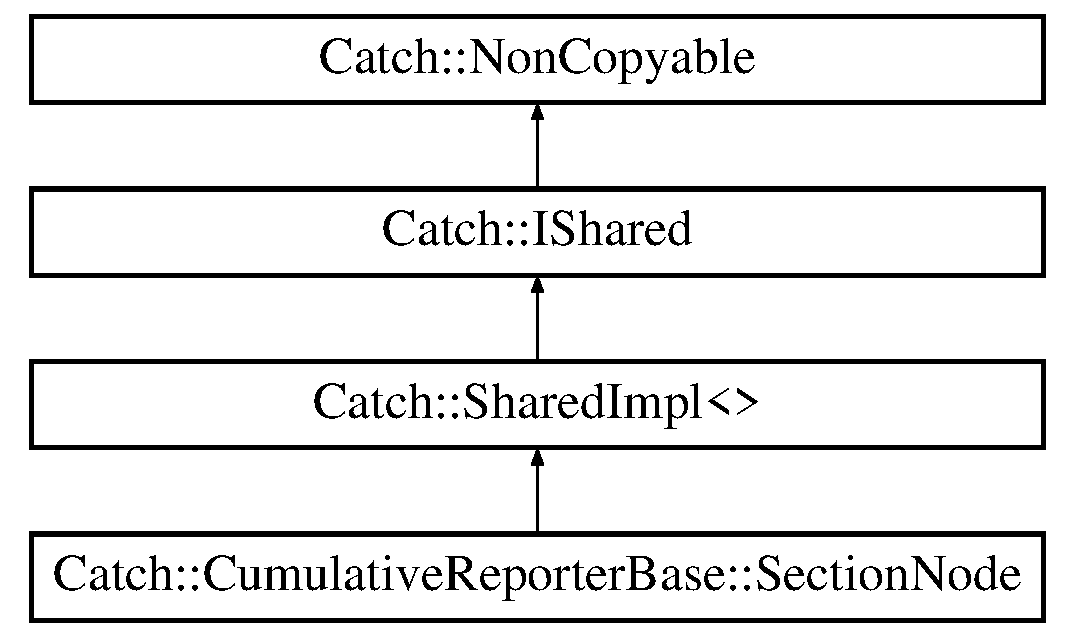
\includegraphics[height=4.000000cm]{struct_catch_1_1_cumulative_reporter_base_1_1_section_node}
\end{center}
\end{figure}
\subsection*{Public Types}
\begin{DoxyCompactItemize}
\item 
\hypertarget{struct_catch_1_1_cumulative_reporter_base_1_1_section_node_adb1744ebcada97d26047ecbdc2d55dd6}{typedef std\-::vector$<$ \hyperlink{class_catch_1_1_ptr}{Ptr}\\*
$<$ \hyperlink{struct_catch_1_1_cumulative_reporter_base_1_1_section_node}{Section\-Node} $>$ $>$ {\bfseries Child\-Sections}}\label{struct_catch_1_1_cumulative_reporter_base_1_1_section_node_adb1744ebcada97d26047ecbdc2d55dd6}

\item 
\hypertarget{struct_catch_1_1_cumulative_reporter_base_1_1_section_node_a55613e2ef8a65bb1fc1f53504ffecb18}{typedef std\-::vector\\*
$<$ \hyperlink{struct_catch_1_1_assertion_stats}{Assertion\-Stats} $>$ {\bfseries Assertions}}\label{struct_catch_1_1_cumulative_reporter_base_1_1_section_node_a55613e2ef8a65bb1fc1f53504ffecb18}

\end{DoxyCompactItemize}
\subsection*{Public Member Functions}
\begin{DoxyCompactItemize}
\item 
\hypertarget{struct_catch_1_1_cumulative_reporter_base_1_1_section_node_adee3ee947f61300bc72266ee007cc1bd}{{\bfseries Section\-Node} (\hyperlink{struct_catch_1_1_section_stats}{Section\-Stats} const \&\-\_\-stats)}\label{struct_catch_1_1_cumulative_reporter_base_1_1_section_node_adee3ee947f61300bc72266ee007cc1bd}

\item 
\hypertarget{struct_catch_1_1_cumulative_reporter_base_1_1_section_node_a4e852b8db8f2ca9da3f2306e6d1099f0}{bool {\bfseries operator==} (\hyperlink{struct_catch_1_1_cumulative_reporter_base_1_1_section_node}{Section\-Node} const \&other) const }\label{struct_catch_1_1_cumulative_reporter_base_1_1_section_node_a4e852b8db8f2ca9da3f2306e6d1099f0}

\item 
\hypertarget{struct_catch_1_1_cumulative_reporter_base_1_1_section_node_a9e66ed9cd0cc7a124270d544340991c0}{bool {\bfseries operator==} (\hyperlink{class_catch_1_1_ptr}{Ptr}$<$ \hyperlink{struct_catch_1_1_cumulative_reporter_base_1_1_section_node}{Section\-Node} $>$ const \&other) const }\label{struct_catch_1_1_cumulative_reporter_base_1_1_section_node_a9e66ed9cd0cc7a124270d544340991c0}

\end{DoxyCompactItemize}
\subsection*{Public Attributes}
\begin{DoxyCompactItemize}
\item 
\hypertarget{struct_catch_1_1_cumulative_reporter_base_1_1_section_node_ace54e2e5f29aad1484bfe501478ef686}{\hyperlink{struct_catch_1_1_section_stats}{Section\-Stats} {\bfseries stats}}\label{struct_catch_1_1_cumulative_reporter_base_1_1_section_node_ace54e2e5f29aad1484bfe501478ef686}

\item 
\hypertarget{struct_catch_1_1_cumulative_reporter_base_1_1_section_node_a755985897fd2694f9589858050a6cf38}{Child\-Sections {\bfseries child\-Sections}}\label{struct_catch_1_1_cumulative_reporter_base_1_1_section_node_a755985897fd2694f9589858050a6cf38}

\item 
\hypertarget{struct_catch_1_1_cumulative_reporter_base_1_1_section_node_a23ea83087a7036ad79e822534cfc5b25}{Assertions {\bfseries assertions}}\label{struct_catch_1_1_cumulative_reporter_base_1_1_section_node_a23ea83087a7036ad79e822534cfc5b25}

\item 
\hypertarget{struct_catch_1_1_cumulative_reporter_base_1_1_section_node_afc6a8c08567d60bb612133632d2992a3}{std\-::string {\bfseries std\-Out}}\label{struct_catch_1_1_cumulative_reporter_base_1_1_section_node_afc6a8c08567d60bb612133632d2992a3}

\item 
\hypertarget{struct_catch_1_1_cumulative_reporter_base_1_1_section_node_ae8e8c7ef27b55ef96d0f15af231fdfb8}{std\-::string {\bfseries std\-Err}}\label{struct_catch_1_1_cumulative_reporter_base_1_1_section_node_ae8e8c7ef27b55ef96d0f15af231fdfb8}

\end{DoxyCompactItemize}


The documentation for this struct was generated from the following file\-:\begin{DoxyCompactItemize}
\item 
Catch.\-h\end{DoxyCompactItemize}

\hypertarget{struct_catch_1_1_section_stats}{\section{Catch\-:\-:Section\-Stats Struct Reference}
\label{struct_catch_1_1_section_stats}\index{Catch\-::\-Section\-Stats@{Catch\-::\-Section\-Stats}}
}
\subsection*{Public Member Functions}
\begin{DoxyCompactItemize}
\item 
\hypertarget{struct_catch_1_1_section_stats_abadf375cb596682e34781b606eb10bfe}{{\bfseries Section\-Stats} (\hyperlink{struct_catch_1_1_section_info}{Section\-Info} const \&\-\_\-section\-Info, \hyperlink{struct_catch_1_1_counts}{Counts} const \&\-\_\-assertions, double \-\_\-duration\-In\-Seconds, bool \-\_\-missing\-Assertions)}\label{struct_catch_1_1_section_stats_abadf375cb596682e34781b606eb10bfe}

\end{DoxyCompactItemize}
\subsection*{Public Attributes}
\begin{DoxyCompactItemize}
\item 
\hypertarget{struct_catch_1_1_section_stats_a524d0cd3b91acc6a4d0f24d6e50275bb}{\hyperlink{struct_catch_1_1_section_info}{Section\-Info} {\bfseries section\-Info}}\label{struct_catch_1_1_section_stats_a524d0cd3b91acc6a4d0f24d6e50275bb}

\item 
\hypertarget{struct_catch_1_1_section_stats_a789bbc5c115f2914286458d282430685}{\hyperlink{struct_catch_1_1_counts}{Counts} {\bfseries assertions}}\label{struct_catch_1_1_section_stats_a789bbc5c115f2914286458d282430685}

\item 
\hypertarget{struct_catch_1_1_section_stats_ae3276a60071b4221907a571b822b0a94}{double {\bfseries duration\-In\-Seconds}}\label{struct_catch_1_1_section_stats_ae3276a60071b4221907a571b822b0a94}

\item 
\hypertarget{struct_catch_1_1_section_stats_a4840f83088787653a656c98e664e6b51}{bool {\bfseries missing\-Assertions}}\label{struct_catch_1_1_section_stats_a4840f83088787653a656c98e664e6b51}

\end{DoxyCompactItemize}


The documentation for this struct was generated from the following file\-:\begin{DoxyCompactItemize}
\item 
Catch.\-h\end{DoxyCompactItemize}

\hypertarget{struct_catch_1_1_shared_impl}{\section{Catch\-:\-:Shared\-Impl$<$ T $>$ Struct Template Reference}
\label{struct_catch_1_1_shared_impl}\index{Catch\-::\-Shared\-Impl$<$ T $>$@{Catch\-::\-Shared\-Impl$<$ T $>$}}
}
Inheritance diagram for Catch\-:\-:Shared\-Impl$<$ T $>$\-:\begin{figure}[H]
\begin{center}
\leavevmode
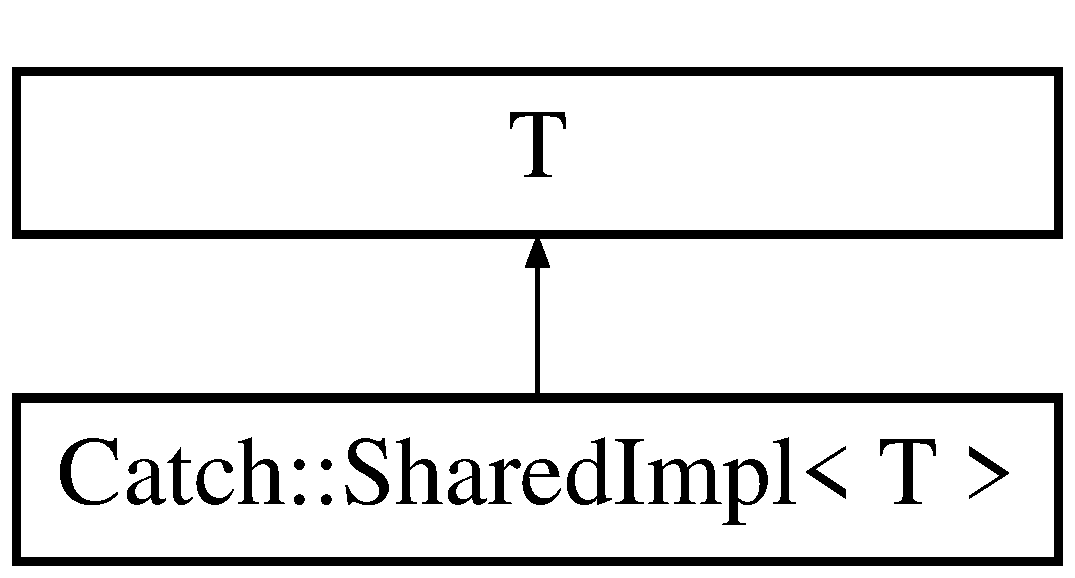
\includegraphics[height=2.000000cm]{struct_catch_1_1_shared_impl}
\end{center}
\end{figure}
\subsection*{Public Member Functions}
\begin{DoxyCompactItemize}
\item 
\hypertarget{struct_catch_1_1_shared_impl_a9b190b7a139a09d2624d1201d8e4f87e}{virtual void {\bfseries add\-Ref} () const }\label{struct_catch_1_1_shared_impl_a9b190b7a139a09d2624d1201d8e4f87e}

\item 
\hypertarget{struct_catch_1_1_shared_impl_a16baad80ad5ad3dfaf2a10a157a02e01}{virtual void {\bfseries release} () const }\label{struct_catch_1_1_shared_impl_a16baad80ad5ad3dfaf2a10a157a02e01}

\end{DoxyCompactItemize}
\subsection*{Public Attributes}
\begin{DoxyCompactItemize}
\item 
\hypertarget{struct_catch_1_1_shared_impl_a7e71ef1985b85aa41a1632f932a96bcb}{unsigned int {\bfseries m\-\_\-rc}}\label{struct_catch_1_1_shared_impl_a7e71ef1985b85aa41a1632f932a96bcb}

\end{DoxyCompactItemize}


The documentation for this struct was generated from the following file\-:\begin{DoxyCompactItemize}
\item 
Catch.\-h\end{DoxyCompactItemize}

\hypertarget{struct_catch_1_1_show_durations}{\section{Catch\-:\-:Show\-Durations Struct Reference}
\label{struct_catch_1_1_show_durations}\index{Catch\-::\-Show\-Durations@{Catch\-::\-Show\-Durations}}
}
\subsection*{Public Types}
\begin{DoxyCompactItemize}
\item 
enum {\bfseries Or\-Not} \{ {\bfseries Default\-For\-Reporter}, 
{\bfseries Always}, 
{\bfseries Never}
 \}
\end{DoxyCompactItemize}


The documentation for this struct was generated from the following file\-:\begin{DoxyCompactItemize}
\item 
Catch.\-h\end{DoxyCompactItemize}

\hypertarget{struct_catch_1_1_source_line_info}{\section{Catch\-:\-:Source\-Line\-Info Struct Reference}
\label{struct_catch_1_1_source_line_info}\index{Catch\-::\-Source\-Line\-Info@{Catch\-::\-Source\-Line\-Info}}
}
\subsection*{Public Member Functions}
\begin{DoxyCompactItemize}
\item 
\hypertarget{struct_catch_1_1_source_line_info_ad75af709941dae9fcb07b7c5cd18294f}{{\bfseries Source\-Line\-Info} (std\-::string const \&\-\_\-file, std\-::size\-\_\-t \-\_\-line)}\label{struct_catch_1_1_source_line_info_ad75af709941dae9fcb07b7c5cd18294f}

\item 
\hypertarget{struct_catch_1_1_source_line_info_a1ec99cc0547ce5909133aaa8f14ed4b1}{{\bfseries Source\-Line\-Info} (\hyperlink{struct_catch_1_1_source_line_info}{Source\-Line\-Info} const \&other)}\label{struct_catch_1_1_source_line_info_a1ec99cc0547ce5909133aaa8f14ed4b1}

\item 
\hypertarget{struct_catch_1_1_source_line_info_a9a25ffc0640d1a3dd0c9b7e5fcbba7b9}{bool {\bfseries empty} () const }\label{struct_catch_1_1_source_line_info_a9a25ffc0640d1a3dd0c9b7e5fcbba7b9}

\item 
\hypertarget{struct_catch_1_1_source_line_info_af0854821b1abfda52796ef0f1294b050}{bool {\bfseries operator==} (\hyperlink{struct_catch_1_1_source_line_info}{Source\-Line\-Info} const \&other) const }\label{struct_catch_1_1_source_line_info_af0854821b1abfda52796ef0f1294b050}

\end{DoxyCompactItemize}
\subsection*{Public Attributes}
\begin{DoxyCompactItemize}
\item 
\hypertarget{struct_catch_1_1_source_line_info_adf3ccf0c2bd326eb3466318af82a94dd}{std\-::string {\bfseries file}}\label{struct_catch_1_1_source_line_info_adf3ccf0c2bd326eb3466318af82a94dd}

\item 
\hypertarget{struct_catch_1_1_source_line_info_a841e5d696c7b9cde24e45e61dd979c77}{std\-::size\-\_\-t {\bfseries line}}\label{struct_catch_1_1_source_line_info_a841e5d696c7b9cde24e45e61dd979c77}

\end{DoxyCompactItemize}


The documentation for this struct was generated from the following file\-:\begin{DoxyCompactItemize}
\item 
Catch.\-h\end{DoxyCompactItemize}

\hypertarget{struct_catch_1_1_matchers_1_1_impl_1_1_std_string_1_1_starts_with}{\section{Catch\-:\-:Matchers\-:\-:Impl\-:\-:Std\-String\-:\-:Starts\-With Struct Reference}
\label{struct_catch_1_1_matchers_1_1_impl_1_1_std_string_1_1_starts_with}\index{Catch\-::\-Matchers\-::\-Impl\-::\-Std\-String\-::\-Starts\-With@{Catch\-::\-Matchers\-::\-Impl\-::\-Std\-String\-::\-Starts\-With}}
}
Inheritance diagram for Catch\-:\-:Matchers\-:\-:Impl\-:\-:Std\-String\-:\-:Starts\-With\-:\begin{figure}[H]
\begin{center}
\leavevmode
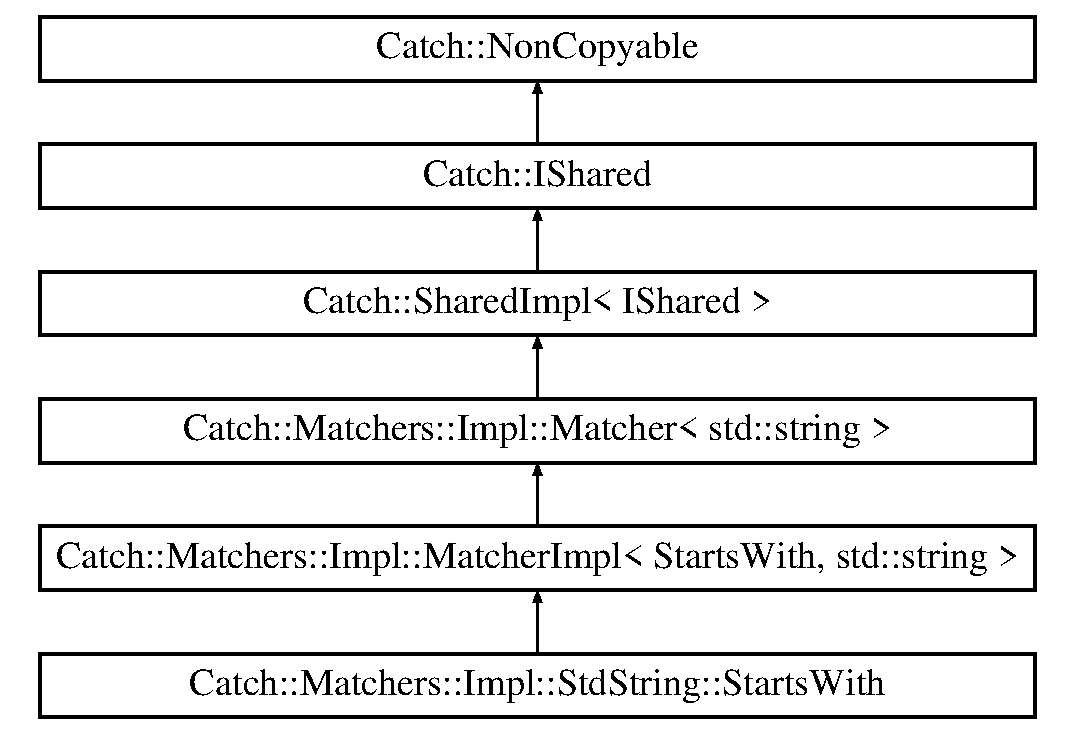
\includegraphics[height=6.000000cm]{struct_catch_1_1_matchers_1_1_impl_1_1_std_string_1_1_starts_with}
\end{center}
\end{figure}
\subsection*{Public Member Functions}
\begin{DoxyCompactItemize}
\item 
\hypertarget{struct_catch_1_1_matchers_1_1_impl_1_1_std_string_1_1_starts_with_a1940dacb184d129adb33acea73dedc17}{{\bfseries Starts\-With} (std\-::string const \&substr)}\label{struct_catch_1_1_matchers_1_1_impl_1_1_std_string_1_1_starts_with_a1940dacb184d129adb33acea73dedc17}

\item 
\hypertarget{struct_catch_1_1_matchers_1_1_impl_1_1_std_string_1_1_starts_with_a5526cb587632e7e46253d6f60ae01098}{{\bfseries Starts\-With} (\hyperlink{struct_catch_1_1_matchers_1_1_impl_1_1_std_string_1_1_starts_with}{Starts\-With} const \&other)}\label{struct_catch_1_1_matchers_1_1_impl_1_1_std_string_1_1_starts_with_a5526cb587632e7e46253d6f60ae01098}

\item 
\hypertarget{struct_catch_1_1_matchers_1_1_impl_1_1_std_string_1_1_starts_with_ae9c893adbacc853171a488aea5355653}{virtual bool {\bfseries match} (std\-::string const \&expr) const }\label{struct_catch_1_1_matchers_1_1_impl_1_1_std_string_1_1_starts_with_ae9c893adbacc853171a488aea5355653}

\item 
\hypertarget{struct_catch_1_1_matchers_1_1_impl_1_1_std_string_1_1_starts_with_a066fe10e74495cb556abc6895193ba97}{virtual std\-::string {\bfseries to\-String} () const }\label{struct_catch_1_1_matchers_1_1_impl_1_1_std_string_1_1_starts_with_a066fe10e74495cb556abc6895193ba97}

\end{DoxyCompactItemize}
\subsection*{Public Attributes}
\begin{DoxyCompactItemize}
\item 
\hypertarget{struct_catch_1_1_matchers_1_1_impl_1_1_std_string_1_1_starts_with_aebcdf35b98fd0097d9e9113b9219fcd1}{std\-::string {\bfseries m\-\_\-substr}}\label{struct_catch_1_1_matchers_1_1_impl_1_1_std_string_1_1_starts_with_aebcdf35b98fd0097d9e9113b9219fcd1}

\end{DoxyCompactItemize}
\subsection*{Additional Inherited Members}


The documentation for this struct was generated from the following file\-:\begin{DoxyCompactItemize}
\item 
Catch.\-h\end{DoxyCompactItemize}

\hypertarget{class_catch_1_1_stream}{\section{Catch\-:\-:Stream Class Reference}
\label{class_catch_1_1_stream}\index{Catch\-::\-Stream@{Catch\-::\-Stream}}
}
\subsection*{Public Member Functions}
\begin{DoxyCompactItemize}
\item 
\hypertarget{class_catch_1_1_stream_a4d2f8a31699cda5e552372e37f78f5dc}{{\bfseries Stream} (std\-::streambuf $\ast$\-\_\-stream\-Buf, bool \-\_\-is\-Owned)}\label{class_catch_1_1_stream_a4d2f8a31699cda5e552372e37f78f5dc}

\item 
\hypertarget{class_catch_1_1_stream_aff188f0e04418234a6a9120a65d058f6}{void {\bfseries release} ()}\label{class_catch_1_1_stream_aff188f0e04418234a6a9120a65d058f6}

\end{DoxyCompactItemize}
\subsection*{Public Attributes}
\begin{DoxyCompactItemize}
\item 
\hypertarget{class_catch_1_1_stream_abd878112035b66f6682e4ba20ee03d72}{std\-::streambuf $\ast$ {\bfseries stream\-Buf}}\label{class_catch_1_1_stream_abd878112035b66f6682e4ba20ee03d72}

\end{DoxyCompactItemize}


The documentation for this class was generated from the following file\-:\begin{DoxyCompactItemize}
\item 
Catch.\-h\end{DoxyCompactItemize}

\hypertarget{class_catch_1_1_stream_buf_base}{\section{Catch\-:\-:Stream\-Buf\-Base Class Reference}
\label{class_catch_1_1_stream_buf_base}\index{Catch\-::\-Stream\-Buf\-Base@{Catch\-::\-Stream\-Buf\-Base}}
}
Inheritance diagram for Catch\-:\-:Stream\-Buf\-Base\-:\begin{figure}[H]
\begin{center}
\leavevmode
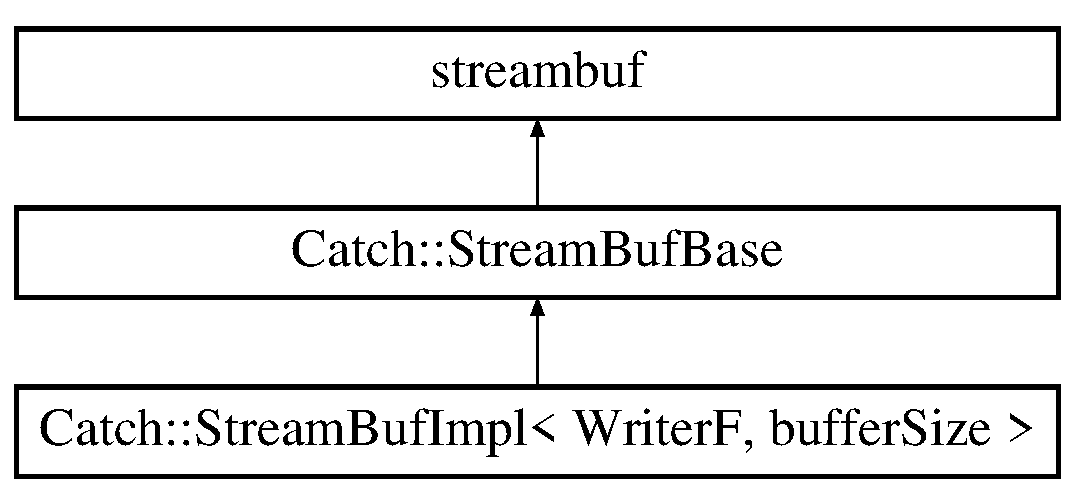
\includegraphics[height=3.000000cm]{class_catch_1_1_stream_buf_base}
\end{center}
\end{figure}


The documentation for this class was generated from the following file\-:\begin{DoxyCompactItemize}
\item 
Catch.\-h\end{DoxyCompactItemize}

\hypertarget{class_catch_1_1_stream_buf_impl}{\section{Catch\-:\-:Stream\-Buf\-Impl$<$ Writer\-F, buffer\-Size $>$ Class Template Reference}
\label{class_catch_1_1_stream_buf_impl}\index{Catch\-::\-Stream\-Buf\-Impl$<$ Writer\-F, buffer\-Size $>$@{Catch\-::\-Stream\-Buf\-Impl$<$ Writer\-F, buffer\-Size $>$}}
}
Inheritance diagram for Catch\-:\-:Stream\-Buf\-Impl$<$ Writer\-F, buffer\-Size $>$\-:\begin{figure}[H]
\begin{center}
\leavevmode
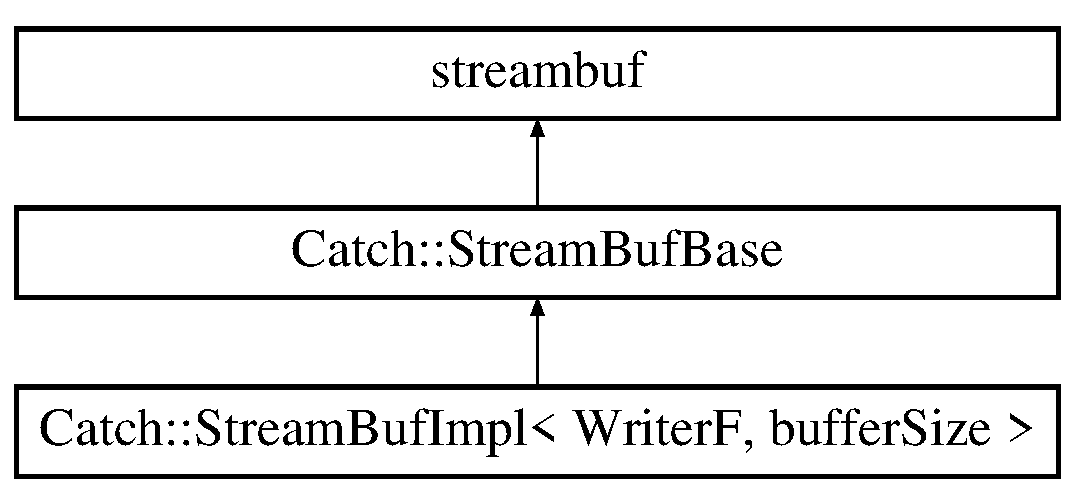
\includegraphics[height=3.000000cm]{class_catch_1_1_stream_buf_impl}
\end{center}
\end{figure}


The documentation for this class was generated from the following file\-:\begin{DoxyCompactItemize}
\item 
Catch.\-h\end{DoxyCompactItemize}

\hypertarget{struct_catch_1_1_streaming_reporter_base}{\section{Catch\-:\-:Streaming\-Reporter\-Base Struct Reference}
\label{struct_catch_1_1_streaming_reporter_base}\index{Catch\-::\-Streaming\-Reporter\-Base@{Catch\-::\-Streaming\-Reporter\-Base}}
}
Inheritance diagram for Catch\-:\-:Streaming\-Reporter\-Base\-:\begin{figure}[H]
\begin{center}
\leavevmode
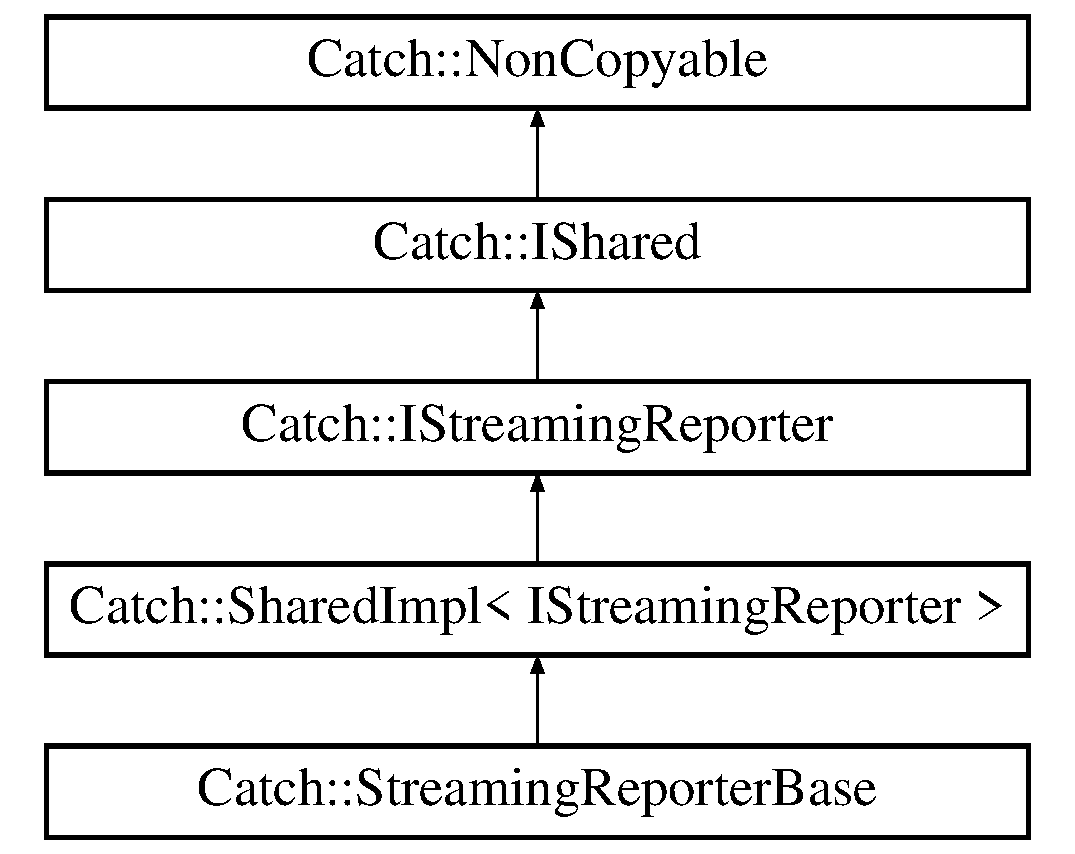
\includegraphics[height=5.000000cm]{struct_catch_1_1_streaming_reporter_base}
\end{center}
\end{figure}
\subsection*{Public Member Functions}
\begin{DoxyCompactItemize}
\item 
\hypertarget{struct_catch_1_1_streaming_reporter_base_a917efb4cef0198b4f2f41f40bfda0459}{{\bfseries Streaming\-Reporter\-Base} (\hyperlink{struct_catch_1_1_reporter_config}{Reporter\-Config} const \&\-\_\-config)}\label{struct_catch_1_1_streaming_reporter_base_a917efb4cef0198b4f2f41f40bfda0459}

\item 
\hypertarget{struct_catch_1_1_streaming_reporter_base_a5f315896a20f8c67274d3587657a4c9e}{virtual void {\bfseries no\-Matching\-Test\-Cases} (std\-::string const \&)}\label{struct_catch_1_1_streaming_reporter_base_a5f315896a20f8c67274d3587657a4c9e}

\item 
\hypertarget{struct_catch_1_1_streaming_reporter_base_a0f97c112f559488dfb998c0e14bde600}{virtual void {\bfseries test\-Run\-Starting} (\hyperlink{struct_catch_1_1_test_run_info}{Test\-Run\-Info} const \&\-\_\-test\-Run\-Info)}\label{struct_catch_1_1_streaming_reporter_base_a0f97c112f559488dfb998c0e14bde600}

\item 
\hypertarget{struct_catch_1_1_streaming_reporter_base_a2731bbea2eb6150d1bed4df25c1a747b}{virtual void {\bfseries test\-Group\-Starting} (\hyperlink{struct_catch_1_1_group_info}{Group\-Info} const \&\-\_\-group\-Info)}\label{struct_catch_1_1_streaming_reporter_base_a2731bbea2eb6150d1bed4df25c1a747b}

\item 
\hypertarget{struct_catch_1_1_streaming_reporter_base_add5764ac7e0a90833d0ef601b09fc52d}{virtual void {\bfseries test\-Case\-Starting} (\hyperlink{struct_catch_1_1_test_case_info}{Test\-Case\-Info} const \&\-\_\-test\-Info)}\label{struct_catch_1_1_streaming_reporter_base_add5764ac7e0a90833d0ef601b09fc52d}

\item 
\hypertarget{struct_catch_1_1_streaming_reporter_base_a5b8de23466f372a7ebd5fe2aa01f5e39}{virtual void {\bfseries section\-Starting} (\hyperlink{struct_catch_1_1_section_info}{Section\-Info} const \&\-\_\-section\-Info)}\label{struct_catch_1_1_streaming_reporter_base_a5b8de23466f372a7ebd5fe2aa01f5e39}

\item 
\hypertarget{struct_catch_1_1_streaming_reporter_base_a6e596fd52cf2a70092fcd45a0c400989}{virtual void {\bfseries section\-Ended} (\hyperlink{struct_catch_1_1_section_stats}{Section\-Stats} const \&)}\label{struct_catch_1_1_streaming_reporter_base_a6e596fd52cf2a70092fcd45a0c400989}

\item 
\hypertarget{struct_catch_1_1_streaming_reporter_base_addb1a3987064941ae03a013cfc855699}{virtual void {\bfseries test\-Case\-Ended} (\hyperlink{struct_catch_1_1_test_case_stats}{Test\-Case\-Stats} const \&)}\label{struct_catch_1_1_streaming_reporter_base_addb1a3987064941ae03a013cfc855699}

\item 
\hypertarget{struct_catch_1_1_streaming_reporter_base_a42fc1d27c45657cba3c60f5c3ed8a3eb}{virtual void {\bfseries test\-Group\-Ended} (\hyperlink{struct_catch_1_1_test_group_stats}{Test\-Group\-Stats} const \&)}\label{struct_catch_1_1_streaming_reporter_base_a42fc1d27c45657cba3c60f5c3ed8a3eb}

\item 
\hypertarget{struct_catch_1_1_streaming_reporter_base_adb6b8987a3402e9365c2150efa563c72}{virtual void {\bfseries test\-Run\-Ended} (\hyperlink{struct_catch_1_1_test_run_stats}{Test\-Run\-Stats} const \&)}\label{struct_catch_1_1_streaming_reporter_base_adb6b8987a3402e9365c2150efa563c72}

\end{DoxyCompactItemize}
\subsection*{Public Attributes}
\begin{DoxyCompactItemize}
\item 
\hypertarget{struct_catch_1_1_streaming_reporter_base_a7d77cac272194543ed81dea9f5c4f3a0}{\hyperlink{class_catch_1_1_ptr}{Ptr}$<$ \hyperlink{struct_catch_1_1_i_config}{I\-Config} $>$ {\bfseries m\-\_\-config}}\label{struct_catch_1_1_streaming_reporter_base_a7d77cac272194543ed81dea9f5c4f3a0}

\item 
\hypertarget{struct_catch_1_1_streaming_reporter_base_aee935c9ec91eca10af8598a88258bde4}{std\-::ostream \& {\bfseries stream}}\label{struct_catch_1_1_streaming_reporter_base_aee935c9ec91eca10af8598a88258bde4}

\item 
\hypertarget{struct_catch_1_1_streaming_reporter_base_af4d83c6abacdbcc7790497f0d50545af}{\hyperlink{struct_catch_1_1_lazy_stat}{Lazy\-Stat}$<$ \hyperlink{struct_catch_1_1_test_run_info}{Test\-Run\-Info} $>$ {\bfseries current\-Test\-Run\-Info}}\label{struct_catch_1_1_streaming_reporter_base_af4d83c6abacdbcc7790497f0d50545af}

\item 
\hypertarget{struct_catch_1_1_streaming_reporter_base_aae9f9ccd5346f51d378fc19d5de5d868}{\hyperlink{struct_catch_1_1_lazy_stat}{Lazy\-Stat}$<$ \hyperlink{struct_catch_1_1_group_info}{Group\-Info} $>$ {\bfseries current\-Group\-Info}}\label{struct_catch_1_1_streaming_reporter_base_aae9f9ccd5346f51d378fc19d5de5d868}

\item 
\hypertarget{struct_catch_1_1_streaming_reporter_base_a8bd70da6d93c21962a2628c3e84991b5}{\hyperlink{struct_catch_1_1_lazy_stat}{Lazy\-Stat}$<$ \hyperlink{struct_catch_1_1_test_case_info}{Test\-Case\-Info} $>$ {\bfseries current\-Test\-Case\-Info}}\label{struct_catch_1_1_streaming_reporter_base_a8bd70da6d93c21962a2628c3e84991b5}

\item 
\hypertarget{struct_catch_1_1_streaming_reporter_base_a82f2a7a5dec58bc093f6ab26a9e47bd8}{std\-::vector$<$ \hyperlink{struct_catch_1_1_section_info}{Section\-Info} $>$ {\bfseries m\-\_\-section\-Stack}}\label{struct_catch_1_1_streaming_reporter_base_a82f2a7a5dec58bc093f6ab26a9e47bd8}

\end{DoxyCompactItemize}


The documentation for this struct was generated from the following file\-:\begin{DoxyCompactItemize}
\item 
Catch.\-h\end{DoxyCompactItemize}

\hypertarget{struct_catch_1_1_string_maker}{\section{Catch\-:\-:String\-Maker$<$ T $>$ Struct Template Reference}
\label{struct_catch_1_1_string_maker}\index{Catch\-::\-String\-Maker$<$ T $>$@{Catch\-::\-String\-Maker$<$ T $>$}}
}
Inheritance diagram for Catch\-:\-:String\-Maker$<$ T $>$\-:\begin{figure}[H]
\begin{center}
\leavevmode
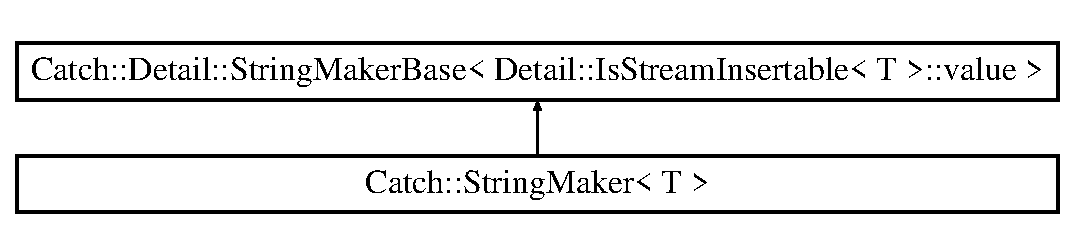
\includegraphics[height=2.000000cm]{struct_catch_1_1_string_maker}
\end{center}
\end{figure}
\subsection*{Additional Inherited Members}


The documentation for this struct was generated from the following file\-:\begin{DoxyCompactItemize}
\item 
Catch.\-h\end{DoxyCompactItemize}

\hypertarget{struct_catch_1_1_string_maker_3_01std_1_1vector_3_01_t_00_01_allocator_01_4_01_4}{\section{Catch\-:\-:String\-Maker$<$ std\-:\-:vector$<$ T, Allocator $>$ $>$ Struct Template Reference}
\label{struct_catch_1_1_string_maker_3_01std_1_1vector_3_01_t_00_01_allocator_01_4_01_4}\index{Catch\-::\-String\-Maker$<$ std\-::vector$<$ T, Allocator $>$ $>$@{Catch\-::\-String\-Maker$<$ std\-::vector$<$ T, Allocator $>$ $>$}}
}
\subsection*{Static Public Member Functions}
\begin{DoxyCompactItemize}
\item 
\hypertarget{struct_catch_1_1_string_maker_3_01std_1_1vector_3_01_t_00_01_allocator_01_4_01_4_adc7dc716733cea8777497257ae22e62d}{static std\-::string {\bfseries convert} (std\-::vector$<$ T, Allocator $>$ const \&v)}\label{struct_catch_1_1_string_maker_3_01std_1_1vector_3_01_t_00_01_allocator_01_4_01_4_adc7dc716733cea8777497257ae22e62d}

\end{DoxyCompactItemize}


The documentation for this struct was generated from the following file\-:\begin{DoxyCompactItemize}
\item 
Catch.\-h\end{DoxyCompactItemize}

\hypertarget{struct_catch_1_1_string_maker_3_01_t_01_5_01_4}{\section{Catch\-:\-:String\-Maker$<$ T $\ast$ $>$ Struct Template Reference}
\label{struct_catch_1_1_string_maker_3_01_t_01_5_01_4}\index{Catch\-::\-String\-Maker$<$ T $\ast$ $>$@{Catch\-::\-String\-Maker$<$ T $\ast$ $>$}}
}
\subsection*{Static Public Member Functions}
\begin{DoxyCompactItemize}
\item 
\hypertarget{struct_catch_1_1_string_maker_3_01_t_01_5_01_4_a2adbc75c99d71b8323f4052bcb0815c9}{{\footnotesize template$<$typename U $>$ }\\static std\-::string {\bfseries convert} (U $\ast$p)}\label{struct_catch_1_1_string_maker_3_01_t_01_5_01_4_a2adbc75c99d71b8323f4052bcb0815c9}

\end{DoxyCompactItemize}


The documentation for this struct was generated from the following file\-:\begin{DoxyCompactItemize}
\item 
Catch.\-h\end{DoxyCompactItemize}

\hypertarget{struct_catch_1_1_detail_1_1_string_maker_base}{\section{Catch\-:\-:Detail\-:\-:String\-Maker\-Base$<$ C $>$ Struct Template Reference}
\label{struct_catch_1_1_detail_1_1_string_maker_base}\index{Catch\-::\-Detail\-::\-String\-Maker\-Base$<$ C $>$@{Catch\-::\-Detail\-::\-String\-Maker\-Base$<$ C $>$}}
}
\subsection*{Static Public Member Functions}
\begin{DoxyCompactItemize}
\item 
\hypertarget{struct_catch_1_1_detail_1_1_string_maker_base_a8eb9f635dc413a5758e22614bafaf1a3}{{\footnotesize template$<$typename T $>$ }\\static std\-::string {\bfseries convert} (T const \&)}\label{struct_catch_1_1_detail_1_1_string_maker_base_a8eb9f635dc413a5758e22614bafaf1a3}

\end{DoxyCompactItemize}


The documentation for this struct was generated from the following file\-:\begin{DoxyCompactItemize}
\item 
Catch.\-h\end{DoxyCompactItemize}

\hypertarget{struct_catch_1_1_detail_1_1_string_maker_base_3_01true_01_4}{\section{Catch\-:\-:Detail\-:\-:String\-Maker\-Base$<$ true $>$ Struct Template Reference}
\label{struct_catch_1_1_detail_1_1_string_maker_base_3_01true_01_4}\index{Catch\-::\-Detail\-::\-String\-Maker\-Base$<$ true $>$@{Catch\-::\-Detail\-::\-String\-Maker\-Base$<$ true $>$}}
}
\subsection*{Static Public Member Functions}
\begin{DoxyCompactItemize}
\item 
\hypertarget{struct_catch_1_1_detail_1_1_string_maker_base_3_01true_01_4_af9b5fdf7fddd8c5c873caa819e5f00f6}{{\footnotesize template$<$typename T $>$ }\\static std\-::string {\bfseries convert} (T const \&\-\_\-value)}\label{struct_catch_1_1_detail_1_1_string_maker_base_3_01true_01_4_af9b5fdf7fddd8c5c873caa819e5f00f6}

\end{DoxyCompactItemize}


The documentation for this struct was generated from the following file\-:\begin{DoxyCompactItemize}
\item 
Catch.\-h\end{DoxyCompactItemize}

\hypertarget{class_catch_1_1_tag}{\section{Catch\-:\-:Tag Class Reference}
\label{class_catch_1_1_tag}\index{Catch\-::\-Tag@{Catch\-::\-Tag}}
}
\subsection*{Public Member Functions}
\begin{DoxyCompactItemize}
\item 
\hypertarget{class_catch_1_1_tag_a3d43477e0f15d4baddc6f6d0943294ae}{{\bfseries Tag} (std\-::string const \&name, bool is\-Negated)}\label{class_catch_1_1_tag_a3d43477e0f15d4baddc6f6d0943294ae}

\item 
\hypertarget{class_catch_1_1_tag_a4fabe27cb327c3221cf9f93573aaae96}{std\-::string {\bfseries get\-Name} () const }\label{class_catch_1_1_tag_a4fabe27cb327c3221cf9f93573aaae96}

\item 
\hypertarget{class_catch_1_1_tag_a437011d6ba5afc54c0e6649b7a200f26}{bool {\bfseries is\-Negated} () const }\label{class_catch_1_1_tag_a437011d6ba5afc54c0e6649b7a200f26}

\item 
\hypertarget{class_catch_1_1_tag_aebcc5d6af02cbfdb27c6e9a0718787fa}{bool {\bfseries operator!} () const }\label{class_catch_1_1_tag_aebcc5d6af02cbfdb27c6e9a0718787fa}

\end{DoxyCompactItemize}


The documentation for this class was generated from the following file\-:\begin{DoxyCompactItemize}
\item 
Catch.\-h\end{DoxyCompactItemize}

\hypertarget{class_catch_1_1_tag_expression}{\section{Catch\-:\-:Tag\-Expression Class Reference}
\label{class_catch_1_1_tag_expression}\index{Catch\-::\-Tag\-Expression@{Catch\-::\-Tag\-Expression}}
}
\subsection*{Public Member Functions}
\begin{DoxyCompactItemize}
\item 
\hypertarget{class_catch_1_1_tag_expression_a723a46b4d0fd6c06a293b6f7ce116f71}{bool {\bfseries matches} (std\-::set$<$ std\-::string $>$ const \&tags) const }\label{class_catch_1_1_tag_expression_a723a46b4d0fd6c06a293b6f7ce116f71}

\end{DoxyCompactItemize}
\subsection*{Friends}
\begin{DoxyCompactItemize}
\item 
\hypertarget{class_catch_1_1_tag_expression_a73ab9a7179a1b439fb9a97d1fa322e7a}{class {\bfseries Tag\-Expression\-Parser}}\label{class_catch_1_1_tag_expression_a73ab9a7179a1b439fb9a97d1fa322e7a}

\end{DoxyCompactItemize}


The documentation for this class was generated from the following file\-:\begin{DoxyCompactItemize}
\item 
Catch.\-h\end{DoxyCompactItemize}

\hypertarget{class_catch_1_1_tag_expression_parser}{\section{Catch\-:\-:Tag\-Expression\-Parser Class Reference}
\label{class_catch_1_1_tag_expression_parser}\index{Catch\-::\-Tag\-Expression\-Parser@{Catch\-::\-Tag\-Expression\-Parser}}
}
Inheritance diagram for Catch\-:\-:Tag\-Expression\-Parser\-:\begin{figure}[H]
\begin{center}
\leavevmode
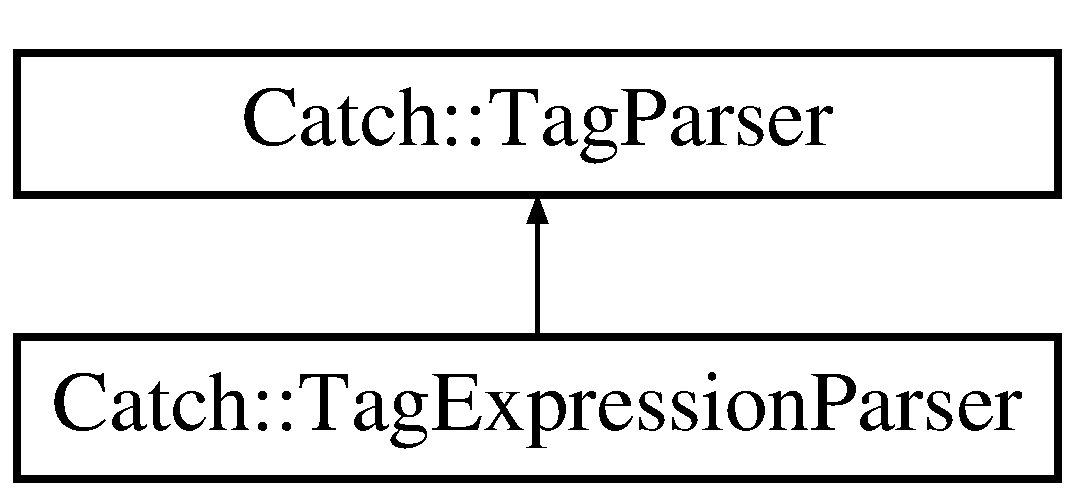
\includegraphics[height=2.000000cm]{class_catch_1_1_tag_expression_parser}
\end{center}
\end{figure}
\subsection*{Public Member Functions}
\begin{DoxyCompactItemize}
\item 
\hypertarget{class_catch_1_1_tag_expression_parser_aeca33975125f6e824c2351312115a8a8}{{\bfseries Tag\-Expression\-Parser} (\hyperlink{class_catch_1_1_tag_expression}{Tag\-Expression} \&exp)}\label{class_catch_1_1_tag_expression_parser_aeca33975125f6e824c2351312115a8a8}

\end{DoxyCompactItemize}


The documentation for this class was generated from the following file\-:\begin{DoxyCompactItemize}
\item 
Catch.\-h\end{DoxyCompactItemize}

\hypertarget{class_catch_1_1_tag_extracter}{\section{Catch\-:\-:Tag\-Extracter Class Reference}
\label{class_catch_1_1_tag_extracter}\index{Catch\-::\-Tag\-Extracter@{Catch\-::\-Tag\-Extracter}}
}
Inheritance diagram for Catch\-:\-:Tag\-Extracter\-:\begin{figure}[H]
\begin{center}
\leavevmode
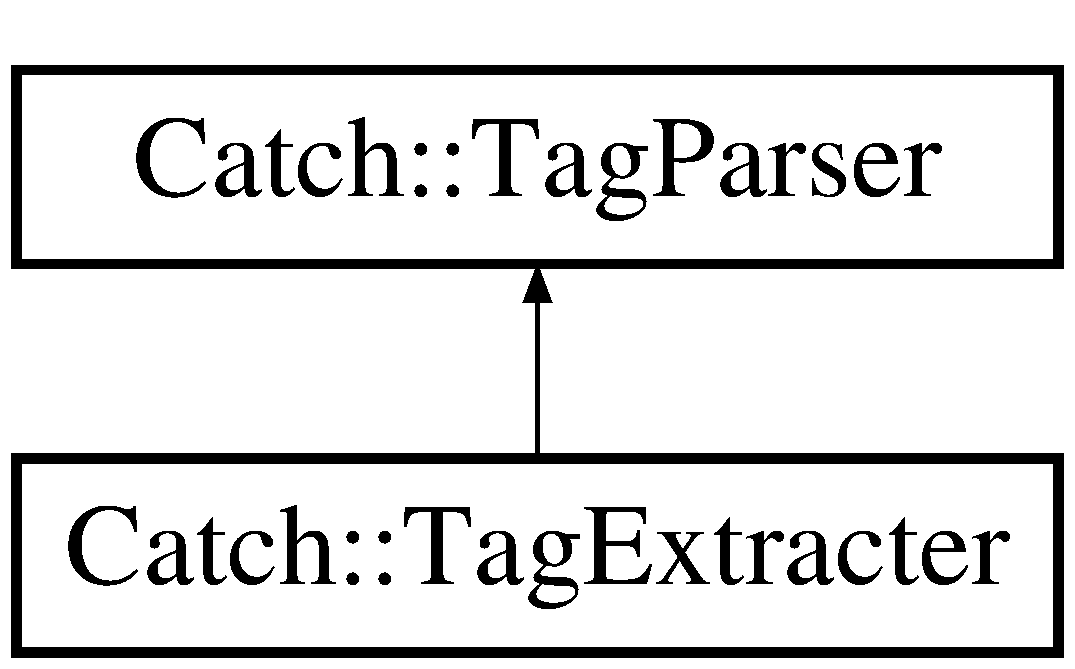
\includegraphics[height=2.000000cm]{class_catch_1_1_tag_extracter}
\end{center}
\end{figure}
\subsection*{Public Member Functions}
\begin{DoxyCompactItemize}
\item 
\hypertarget{class_catch_1_1_tag_extracter_a146d1ab5e247d5ec7c2c61a8c59b7950}{{\bfseries Tag\-Extracter} (std\-::set$<$ std\-::string $>$ \&tags)}\label{class_catch_1_1_tag_extracter_a146d1ab5e247d5ec7c2c61a8c59b7950}

\item 
\hypertarget{class_catch_1_1_tag_extracter_a2f9446590db696802be81b0f743bf9f6}{void {\bfseries parse} (std\-::string \&description)}\label{class_catch_1_1_tag_extracter_a2f9446590db696802be81b0f743bf9f6}

\end{DoxyCompactItemize}
\subsection*{Additional Inherited Members}


The documentation for this class was generated from the following file\-:\begin{DoxyCompactItemize}
\item 
Catch.\-h\end{DoxyCompactItemize}

\hypertarget{class_catch_1_1_tag_parser}{\section{Catch\-:\-:Tag\-Parser Class Reference}
\label{class_catch_1_1_tag_parser}\index{Catch\-::\-Tag\-Parser@{Catch\-::\-Tag\-Parser}}
}
Inheritance diagram for Catch\-:\-:Tag\-Parser\-:\begin{figure}[H]
\begin{center}
\leavevmode
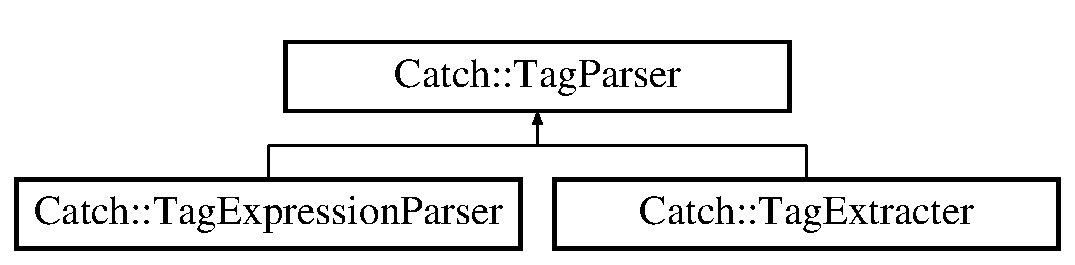
\includegraphics[height=2.000000cm]{class_catch_1_1_tag_parser}
\end{center}
\end{figure}
\subsection*{Public Member Functions}
\begin{DoxyCompactItemize}
\item 
\hypertarget{class_catch_1_1_tag_parser_afc37c4ca179f183d1fa46e703acd244f}{void {\bfseries parse} (std\-::string const \&str)}\label{class_catch_1_1_tag_parser_afc37c4ca179f183d1fa46e703acd244f}

\end{DoxyCompactItemize}
\subsection*{Protected Member Functions}
\begin{DoxyCompactItemize}
\item 
\hypertarget{class_catch_1_1_tag_parser_ad10e947a1e3e23df86cf5d2e7f8ac86b}{virtual void {\bfseries accept\-Tag} (std\-::string const \&tag)=0}\label{class_catch_1_1_tag_parser_ad10e947a1e3e23df86cf5d2e7f8ac86b}

\item 
\hypertarget{class_catch_1_1_tag_parser_a39660c883ef0dc71fc79f067b2832a27}{virtual void {\bfseries accept\-Char} (char c)=0}\label{class_catch_1_1_tag_parser_a39660c883ef0dc71fc79f067b2832a27}

\item 
\hypertarget{class_catch_1_1_tag_parser_ac26ddd9fe8289b13058bb3e96cc6027a}{virtual void {\bfseries end\-Parse} ()}\label{class_catch_1_1_tag_parser_ac26ddd9fe8289b13058bb3e96cc6027a}

\end{DoxyCompactItemize}


The documentation for this class was generated from the following file\-:\begin{DoxyCompactItemize}
\item 
Catch.\-h\end{DoxyCompactItemize}

\hypertarget{class_catch_1_1_tag_set}{\section{Catch\-:\-:Tag\-Set Class Reference}
\label{class_catch_1_1_tag_set}\index{Catch\-::\-Tag\-Set@{Catch\-::\-Tag\-Set}}
}
\subsection*{Public Member Functions}
\begin{DoxyCompactItemize}
\item 
\hypertarget{class_catch_1_1_tag_set_aee4ac50048b95e38ee2ee90cdbd2f2d7}{void {\bfseries add} (\hyperlink{class_catch_1_1_tag}{Tag} const \&tag)}\label{class_catch_1_1_tag_set_aee4ac50048b95e38ee2ee90cdbd2f2d7}

\item 
\hypertarget{class_catch_1_1_tag_set_aaa7ba754671a5ff17261f214adb9164c}{bool {\bfseries empty} () const }\label{class_catch_1_1_tag_set_aaa7ba754671a5ff17261f214adb9164c}

\item 
\hypertarget{class_catch_1_1_tag_set_a33fffe93717ff00ab9552a5e59ebeec1}{bool {\bfseries matches} (std\-::set$<$ std\-::string $>$ const \&tags) const }\label{class_catch_1_1_tag_set_a33fffe93717ff00ab9552a5e59ebeec1}

\end{DoxyCompactItemize}


The documentation for this class was generated from the following file\-:\begin{DoxyCompactItemize}
\item 
Catch.\-h\end{DoxyCompactItemize}

\hypertarget{class_tape}{\section{Tape Class Reference}
\label{class_tape}\index{Tape@{Tape}}
}


Class representing the tape for a Turing Machine.  




{\ttfamily \#include $<$Turing.\-h$>$}

\subsection*{Public Member Functions}
\begin{DoxyCompactItemize}
\item 
\hyperlink{class_tape_ac9e6dc94e43fa247f8b8f4424ac746fb}{Tape} (const std\-::string \&input, char blank, int track\-Count)
\begin{DoxyCompactList}\small\item\em Constructor. \end{DoxyCompactList}\item 
\hypertarget{class_tape_aa50f57d8abf8bead8894cd5c4eeca65e}{std\-::vector$<$ char $>$ {\bfseries get\-Symbols\-At\-Head} () const }\label{class_tape_aa50f57d8abf8bead8894cd5c4eeca65e}

\item 
void \hyperlink{class_tape_a9beaef539c5bb3e9955fc09baf841888}{replace\-Symbols\-At\-Head} (const std\-::vector$<$ char $>$ \&symbols)
\begin{DoxyCompactList}\small\item\em Replaces symbol(s) at given position by given symbol(s) \end{DoxyCompactList}\item 
void \hyperlink{class_tape_afe80b9ce38e3000ededda058ec2bfb9a}{move\-Head} (Direction dir)
\begin{DoxyCompactList}\small\item\em Move head one spot. \end{DoxyCompactList}\end{DoxyCompactItemize}
\subsection*{Friends}
\begin{DoxyCompactItemize}
\item 
\hypertarget{class_tape_afea44fb3a81c1e60cfdb6cd6f9149da8}{std\-::ostream \& \hyperlink{class_tape_afea44fb3a81c1e60cfdb6cd6f9149da8}{operator$<$$<$} (std\-::ostream \&output, const \hyperlink{class_tape}{Tape} \&T)}\label{class_tape_afea44fb3a81c1e60cfdb6cd6f9149da8}

\begin{DoxyCompactList}\small\item\em output overload \end{DoxyCompactList}\end{DoxyCompactItemize}


\subsection{Detailed Description}
Class representing the tape for a Turing Machine. 

\subsection{Constructor \& Destructor Documentation}
\hypertarget{class_tape_ac9e6dc94e43fa247f8b8f4424ac746fb}{\index{Tape@{Tape}!Tape@{Tape}}
\index{Tape@{Tape}!Tape@{Tape}}
\subsubsection[{Tape}]{\setlength{\rightskip}{0pt plus 5cm}Tape\-::\-Tape (
\begin{DoxyParamCaption}
\item[{const std\-::string \&}]{input, }
\item[{char}]{blank, }
\item[{int}]{track\-Count}
\end{DoxyParamCaption}
)}}\label{class_tape_ac9e6dc94e43fa247f8b8f4424ac746fb}


Constructor. 


\begin{DoxyParams}{Parameters}
{\em input} & String to write to tape \\
\hline
{\em blank} & Blank symbol \\
\hline
{\em track\-Count} & number of tracks on the tape \\
\hline
\end{DoxyParams}


\subsection{Member Function Documentation}
\hypertarget{class_tape_afe80b9ce38e3000ededda058ec2bfb9a}{\index{Tape@{Tape}!move\-Head@{move\-Head}}
\index{move\-Head@{move\-Head}!Tape@{Tape}}
\subsubsection[{move\-Head}]{\setlength{\rightskip}{0pt plus 5cm}void Tape\-::move\-Head (
\begin{DoxyParamCaption}
\item[{Direction}]{dir}
\end{DoxyParamCaption}
)}}\label{class_tape_afe80b9ce38e3000ededda058ec2bfb9a}


Move head one spot. 


\begin{DoxyParams}{Parameters}
{\em dir} & Left or right \\
\hline
\end{DoxyParams}
\hypertarget{class_tape_a9beaef539c5bb3e9955fc09baf841888}{\index{Tape@{Tape}!replace\-Symbols\-At\-Head@{replace\-Symbols\-At\-Head}}
\index{replace\-Symbols\-At\-Head@{replace\-Symbols\-At\-Head}!Tape@{Tape}}
\subsubsection[{replace\-Symbols\-At\-Head}]{\setlength{\rightskip}{0pt plus 5cm}void Tape\-::replace\-Symbols\-At\-Head (
\begin{DoxyParamCaption}
\item[{const std\-::vector$<$ char $>$ \&}]{symbols}
\end{DoxyParamCaption}
)}}\label{class_tape_a9beaef539c5bb3e9955fc09baf841888}


Replaces symbol(s) at given position by given symbol(s) 


\begin{DoxyParams}{Parameters}
{\em symbol} & The symbol(s) to be written to tape \\
\hline
\end{DoxyParams}


The documentation for this class was generated from the following files\-:\begin{DoxyCompactItemize}
\item 
Turing.\-h\item 
Turing.\-cpp\end{DoxyCompactItemize}

\hypertarget{class_catch_1_1_test_case}{\section{Catch\-:\-:Test\-Case Class Reference}
\label{class_catch_1_1_test_case}\index{Catch\-::\-Test\-Case@{Catch\-::\-Test\-Case}}
}
Inheritance diagram for Catch\-:\-:Test\-Case\-:\begin{figure}[H]
\begin{center}
\leavevmode
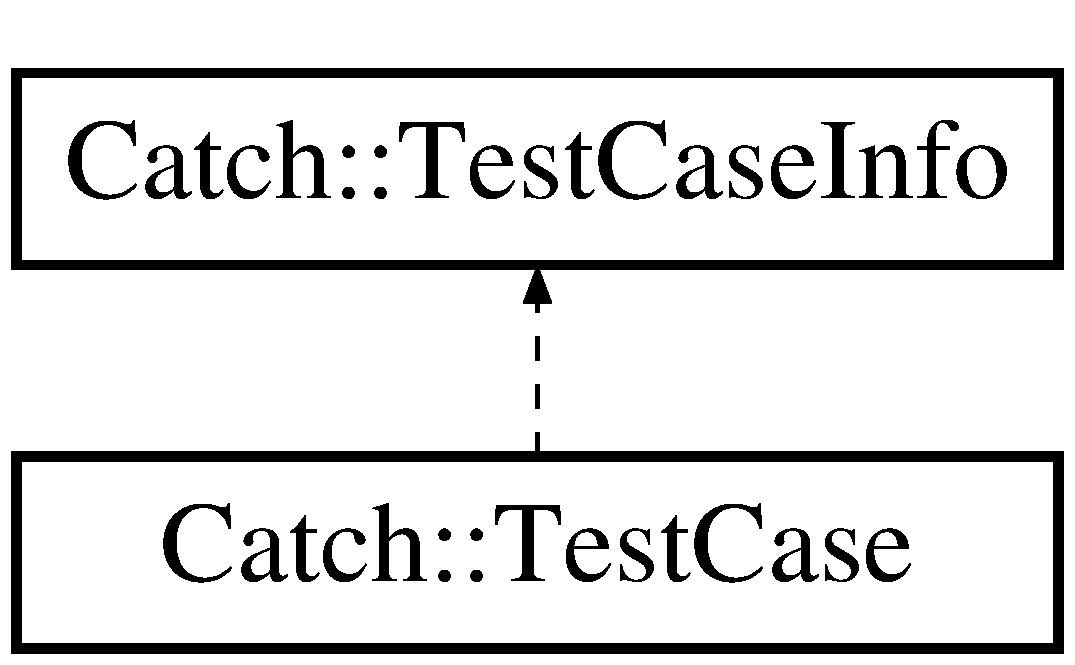
\includegraphics[height=2.000000cm]{class_catch_1_1_test_case}
\end{center}
\end{figure}
\subsection*{Public Member Functions}
\begin{DoxyCompactItemize}
\item 
\hypertarget{class_catch_1_1_test_case_a03a5b913484681bd6d398dc5e9c2a907}{{\bfseries Test\-Case} (\hyperlink{struct_catch_1_1_i_test_case}{I\-Test\-Case} $\ast$test\-Case, \hyperlink{struct_catch_1_1_test_case_info}{Test\-Case\-Info} const \&info)}\label{class_catch_1_1_test_case_a03a5b913484681bd6d398dc5e9c2a907}

\item 
\hypertarget{class_catch_1_1_test_case_ac0011d3789edc3e44edb41f13c4775a0}{{\bfseries Test\-Case} (\hyperlink{class_catch_1_1_test_case}{Test\-Case} const \&other)}\label{class_catch_1_1_test_case_ac0011d3789edc3e44edb41f13c4775a0}

\item 
\hypertarget{class_catch_1_1_test_case_ab6dbc6c82b7c1680013c67bdedccfc8e}{\hyperlink{class_catch_1_1_test_case}{Test\-Case} {\bfseries with\-Name} (std\-::string const \&\-\_\-new\-Name) const }\label{class_catch_1_1_test_case_ab6dbc6c82b7c1680013c67bdedccfc8e}

\item 
\hypertarget{class_catch_1_1_test_case_aac2e028135cc88c3e3aac04650960a6c}{void {\bfseries invoke} () const }\label{class_catch_1_1_test_case_aac2e028135cc88c3e3aac04650960a6c}

\item 
\hypertarget{class_catch_1_1_test_case_a25c03661ab092431cdff10df5c58a5a7}{\hyperlink{struct_catch_1_1_test_case_info}{Test\-Case\-Info} const \& {\bfseries get\-Test\-Case\-Info} () const }\label{class_catch_1_1_test_case_a25c03661ab092431cdff10df5c58a5a7}

\item 
\hypertarget{class_catch_1_1_test_case_a61477cce84066cb77d4eeef5a1470a36}{bool {\bfseries is\-Hidden} () const }\label{class_catch_1_1_test_case_a61477cce84066cb77d4eeef5a1470a36}

\item 
\hypertarget{class_catch_1_1_test_case_ae3c1a0898ee9936cd1d4f207e3903308}{bool {\bfseries has\-Tag} (std\-::string const \&tag) const }\label{class_catch_1_1_test_case_ae3c1a0898ee9936cd1d4f207e3903308}

\item 
\hypertarget{class_catch_1_1_test_case_a89cf3a144b6f256b6a533a631f7a8b0c}{bool {\bfseries matches\-Tags} (std\-::string const \&tag\-Pattern) const }\label{class_catch_1_1_test_case_a89cf3a144b6f256b6a533a631f7a8b0c}

\item 
\hypertarget{class_catch_1_1_test_case_aa4313341335b9a9ebbe4682c0d808b32}{std\-::set$<$ std\-::string $>$ const \& {\bfseries get\-Tags} () const }\label{class_catch_1_1_test_case_aa4313341335b9a9ebbe4682c0d808b32}

\item 
\hypertarget{class_catch_1_1_test_case_aee38f908faf10b905b209ca388275413}{void {\bfseries swap} (\hyperlink{class_catch_1_1_test_case}{Test\-Case} \&other)}\label{class_catch_1_1_test_case_aee38f908faf10b905b209ca388275413}

\item 
\hypertarget{class_catch_1_1_test_case_a40eab521b316c7d476f6b4dd1c33eec8}{bool {\bfseries operator==} (\hyperlink{class_catch_1_1_test_case}{Test\-Case} const \&other) const }\label{class_catch_1_1_test_case_a40eab521b316c7d476f6b4dd1c33eec8}

\item 
\hypertarget{class_catch_1_1_test_case_aa5174e85e3aac6e7398dee9c76730324}{bool {\bfseries operator$<$} (\hyperlink{class_catch_1_1_test_case}{Test\-Case} const \&other) const }\label{class_catch_1_1_test_case_aa5174e85e3aac6e7398dee9c76730324}

\item 
\hypertarget{class_catch_1_1_test_case_a8022e3f74232f7887d2d2cbbc8876502}{\hyperlink{class_catch_1_1_test_case}{Test\-Case} \& {\bfseries operator=} (\hyperlink{class_catch_1_1_test_case}{Test\-Case} const \&other)}\label{class_catch_1_1_test_case_a8022e3f74232f7887d2d2cbbc8876502}

\end{DoxyCompactItemize}
\subsection*{Additional Inherited Members}


The documentation for this class was generated from the following file\-:\begin{DoxyCompactItemize}
\item 
Catch.\-h\end{DoxyCompactItemize}

\hypertarget{class_catch_1_1_test_case_filter}{\section{Catch\-:\-:Test\-Case\-Filter Class Reference}
\label{class_catch_1_1_test_case_filter}\index{Catch\-::\-Test\-Case\-Filter@{Catch\-::\-Test\-Case\-Filter}}
}
\subsection*{Public Member Functions}
\begin{DoxyCompactItemize}
\item 
\hypertarget{class_catch_1_1_test_case_filter_a834f4aaf94f6d4dab0c43db2425e533b}{{\bfseries Test\-Case\-Filter} (std\-::string const \&test\-Spec, If\-Filter\-Matches\-::\-Do\-What match\-Behaviour=If\-Filter\-Matches\-::\-Auto\-Detect\-Behaviour)}\label{class_catch_1_1_test_case_filter_a834f4aaf94f6d4dab0c43db2425e533b}

\item 
\hypertarget{class_catch_1_1_test_case_filter_a27d4b3e5d04034f2bcbb1f070fb55412}{If\-Filter\-Matches\-::\-Do\-What {\bfseries get\-Filter\-Type} () const }\label{class_catch_1_1_test_case_filter_a27d4b3e5d04034f2bcbb1f070fb55412}

\item 
\hypertarget{class_catch_1_1_test_case_filter_a4af367b82ecf4f14d52ad969dcdf0364}{bool {\bfseries should\-Include} (\hyperlink{class_catch_1_1_test_case}{Test\-Case} const \&test\-Case) const }\label{class_catch_1_1_test_case_filter_a4af367b82ecf4f14d52ad969dcdf0364}

\end{DoxyCompactItemize}


The documentation for this class was generated from the following file\-:\begin{DoxyCompactItemize}
\item 
Catch.\-h\end{DoxyCompactItemize}

\hypertarget{class_catch_1_1_test_case_filters}{\section{Catch\-:\-:Test\-Case\-Filters Class Reference}
\label{class_catch_1_1_test_case_filters}\index{Catch\-::\-Test\-Case\-Filters@{Catch\-::\-Test\-Case\-Filters}}
}
\subsection*{Public Member Functions}
\begin{DoxyCompactItemize}
\item 
\hypertarget{class_catch_1_1_test_case_filters_aeaf3582868c07dfae6a31366c7964a92}{{\bfseries Test\-Case\-Filters} (std\-::string const \&name)}\label{class_catch_1_1_test_case_filters_aeaf3582868c07dfae6a31366c7964a92}

\item 
\hypertarget{class_catch_1_1_test_case_filters_a2acf97540f4fc9979a4c46068bc908d6}{std\-::string {\bfseries get\-Name} () const }\label{class_catch_1_1_test_case_filters_a2acf97540f4fc9979a4c46068bc908d6}

\item 
\hypertarget{class_catch_1_1_test_case_filters_a7f1ffd2e932d90a80d6dc6279ff9216d}{void {\bfseries add\-Filter} (\hyperlink{class_catch_1_1_test_case_filter}{Test\-Case\-Filter} const \&filter)}\label{class_catch_1_1_test_case_filters_a7f1ffd2e932d90a80d6dc6279ff9216d}

\item 
\hypertarget{class_catch_1_1_test_case_filters_a77d8212d883341c8de88d01f4c419d83}{void {\bfseries add\-Tags} (std\-::string const \&tag\-Pattern)}\label{class_catch_1_1_test_case_filters_a77d8212d883341c8de88d01f4c419d83}

\item 
\hypertarget{class_catch_1_1_test_case_filters_a8cb88af0aee7449c3409891948e51d3b}{bool {\bfseries should\-Include} (\hyperlink{class_catch_1_1_test_case}{Test\-Case} const \&test\-Case) const }\label{class_catch_1_1_test_case_filters_a8cb88af0aee7449c3409891948e51d3b}

\end{DoxyCompactItemize}


The documentation for this class was generated from the following file\-:\begin{DoxyCompactItemize}
\item 
Catch.\-h\end{DoxyCompactItemize}

\hypertarget{struct_catch_1_1_test_case_info}{\section{Catch\-:\-:Test\-Case\-Info Struct Reference}
\label{struct_catch_1_1_test_case_info}\index{Catch\-::\-Test\-Case\-Info@{Catch\-::\-Test\-Case\-Info}}
}
Inheritance diagram for Catch\-:\-:Test\-Case\-Info\-:\begin{figure}[H]
\begin{center}
\leavevmode
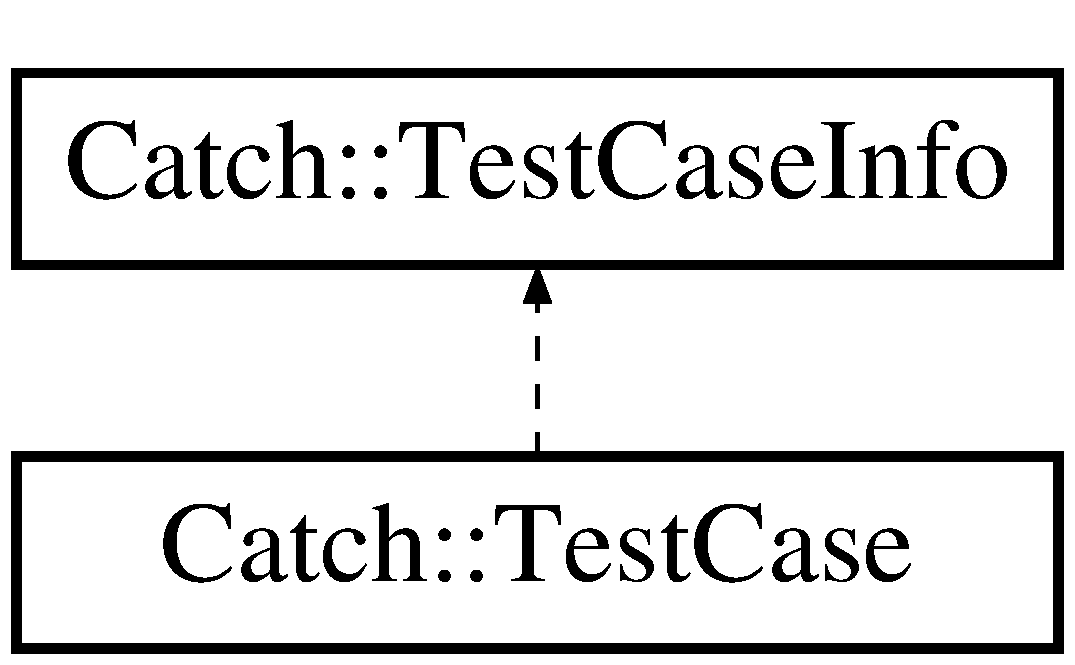
\includegraphics[height=2.000000cm]{struct_catch_1_1_test_case_info}
\end{center}
\end{figure}
\subsection*{Public Member Functions}
\begin{DoxyCompactItemize}
\item 
\hypertarget{struct_catch_1_1_test_case_info_a6bd4c4e3fab75ba12f6592d3e3bf8c34}{{\bfseries Test\-Case\-Info} (std\-::string const \&\-\_\-name, std\-::string const \&\-\_\-class\-Name, std\-::string const \&\-\_\-description, std\-::set$<$ std\-::string $>$ const \&\-\_\-tags, bool \-\_\-is\-Hidden, \hyperlink{struct_catch_1_1_source_line_info}{Source\-Line\-Info} const \&\-\_\-line\-Info)}\label{struct_catch_1_1_test_case_info_a6bd4c4e3fab75ba12f6592d3e3bf8c34}

\item 
\hypertarget{struct_catch_1_1_test_case_info_ac338adb4e38f4bf3977fb45b2b1fe447}{{\bfseries Test\-Case\-Info} (\hyperlink{struct_catch_1_1_test_case_info}{Test\-Case\-Info} const \&other)}\label{struct_catch_1_1_test_case_info_ac338adb4e38f4bf3977fb45b2b1fe447}

\end{DoxyCompactItemize}
\subsection*{Public Attributes}
\begin{DoxyCompactItemize}
\item 
\hypertarget{struct_catch_1_1_test_case_info_a463794e2f5cfead307c93efd134ade36}{std\-::string {\bfseries name}}\label{struct_catch_1_1_test_case_info_a463794e2f5cfead307c93efd134ade36}

\item 
\hypertarget{struct_catch_1_1_test_case_info_a1a5e0825132a38d091defdebbf2f8ce9}{std\-::string {\bfseries class\-Name}}\label{struct_catch_1_1_test_case_info_a1a5e0825132a38d091defdebbf2f8ce9}

\item 
\hypertarget{struct_catch_1_1_test_case_info_a37fe2db9425bc45f6a33893eac31198e}{std\-::string {\bfseries description}}\label{struct_catch_1_1_test_case_info_a37fe2db9425bc45f6a33893eac31198e}

\item 
\hypertarget{struct_catch_1_1_test_case_info_a045f62e7719a8760a5b456f7fd2dc97c}{std\-::set$<$ std\-::string $>$ {\bfseries tags}}\label{struct_catch_1_1_test_case_info_a045f62e7719a8760a5b456f7fd2dc97c}

\item 
\hypertarget{struct_catch_1_1_test_case_info_ac65c2d36fd36f71e9bf782b2ea245c64}{std\-::string {\bfseries tags\-As\-String}}\label{struct_catch_1_1_test_case_info_ac65c2d36fd36f71e9bf782b2ea245c64}

\item 
\hypertarget{struct_catch_1_1_test_case_info_aa9407b7f442655b51a2aad24b3fa2fd3}{\hyperlink{struct_catch_1_1_source_line_info}{Source\-Line\-Info} {\bfseries line\-Info}}\label{struct_catch_1_1_test_case_info_aa9407b7f442655b51a2aad24b3fa2fd3}

\item 
\hypertarget{struct_catch_1_1_test_case_info_a8c4c85cb2e28897721c9f5fe3950bc2f}{bool {\bfseries is\-Hidden}}\label{struct_catch_1_1_test_case_info_a8c4c85cb2e28897721c9f5fe3950bc2f}

\end{DoxyCompactItemize}


The documentation for this struct was generated from the following file\-:\begin{DoxyCompactItemize}
\item 
Catch.\-h\end{DoxyCompactItemize}

\hypertarget{struct_catch_1_1_test_case_stats}{\section{Catch\-:\-:Test\-Case\-Stats Struct Reference}
\label{struct_catch_1_1_test_case_stats}\index{Catch\-::\-Test\-Case\-Stats@{Catch\-::\-Test\-Case\-Stats}}
}
\subsection*{Public Member Functions}
\begin{DoxyCompactItemize}
\item 
\hypertarget{struct_catch_1_1_test_case_stats_ac5000f8751634dc39e48b87bd7e79970}{{\bfseries Test\-Case\-Stats} (\hyperlink{struct_catch_1_1_test_case_info}{Test\-Case\-Info} const \&\-\_\-test\-Info, \hyperlink{struct_catch_1_1_totals}{Totals} const \&\-\_\-totals, std\-::string const \&\-\_\-std\-Out, std\-::string const \&\-\_\-std\-Err, bool \-\_\-aborting)}\label{struct_catch_1_1_test_case_stats_ac5000f8751634dc39e48b87bd7e79970}

\end{DoxyCompactItemize}
\subsection*{Public Attributes}
\begin{DoxyCompactItemize}
\item 
\hypertarget{struct_catch_1_1_test_case_stats_a6eb1ba3f940b899f7734c0f8888c0252}{\hyperlink{struct_catch_1_1_test_case_info}{Test\-Case\-Info} {\bfseries test\-Info}}\label{struct_catch_1_1_test_case_stats_a6eb1ba3f940b899f7734c0f8888c0252}

\item 
\hypertarget{struct_catch_1_1_test_case_stats_afc3947e6c6ca93cad0bdc6742c65c4a8}{\hyperlink{struct_catch_1_1_totals}{Totals} {\bfseries totals}}\label{struct_catch_1_1_test_case_stats_afc3947e6c6ca93cad0bdc6742c65c4a8}

\item 
\hypertarget{struct_catch_1_1_test_case_stats_acab436aeefce581c52d0e195872484f7}{std\-::string {\bfseries std\-Out}}\label{struct_catch_1_1_test_case_stats_acab436aeefce581c52d0e195872484f7}

\item 
\hypertarget{struct_catch_1_1_test_case_stats_a84851abaa94a6b09664517a4919fa8ac}{std\-::string {\bfseries std\-Err}}\label{struct_catch_1_1_test_case_stats_a84851abaa94a6b09664517a4919fa8ac}

\item 
\hypertarget{struct_catch_1_1_test_case_stats_a0b61bf85883cde3d2c294a685aed49e7}{bool {\bfseries aborting}}\label{struct_catch_1_1_test_case_stats_a0b61bf85883cde3d2c294a685aed49e7}

\end{DoxyCompactItemize}


The documentation for this struct was generated from the following file\-:\begin{DoxyCompactItemize}
\item 
Catch.\-h\end{DoxyCompactItemize}

\hypertarget{struct_catch_1_1_test_failure_exception}{\section{Catch\-:\-:Test\-Failure\-Exception Struct Reference}
\label{struct_catch_1_1_test_failure_exception}\index{Catch\-::\-Test\-Failure\-Exception@{Catch\-::\-Test\-Failure\-Exception}}
}


The documentation for this struct was generated from the following file\-:\begin{DoxyCompactItemize}
\item 
Catch.\-h\end{DoxyCompactItemize}

\hypertarget{struct_catch_1_1_test_group_stats}{\section{Catch\-:\-:Test\-Group\-Stats Struct Reference}
\label{struct_catch_1_1_test_group_stats}\index{Catch\-::\-Test\-Group\-Stats@{Catch\-::\-Test\-Group\-Stats}}
}
\subsection*{Public Member Functions}
\begin{DoxyCompactItemize}
\item 
\hypertarget{struct_catch_1_1_test_group_stats_aa3b01aa722be787059bca806e4f10be4}{{\bfseries Test\-Group\-Stats} (\hyperlink{struct_catch_1_1_group_info}{Group\-Info} const \&\-\_\-group\-Info, \hyperlink{struct_catch_1_1_totals}{Totals} const \&\-\_\-totals, bool \-\_\-aborting)}\label{struct_catch_1_1_test_group_stats_aa3b01aa722be787059bca806e4f10be4}

\item 
\hypertarget{struct_catch_1_1_test_group_stats_a2b2bb846beeb23d4dd20b1f5cd7e92bb}{{\bfseries Test\-Group\-Stats} (\hyperlink{struct_catch_1_1_group_info}{Group\-Info} const \&\-\_\-group\-Info)}\label{struct_catch_1_1_test_group_stats_a2b2bb846beeb23d4dd20b1f5cd7e92bb}

\end{DoxyCompactItemize}
\subsection*{Public Attributes}
\begin{DoxyCompactItemize}
\item 
\hypertarget{struct_catch_1_1_test_group_stats_a61c3692541a33e959ad5a0053cdc001b}{\hyperlink{struct_catch_1_1_group_info}{Group\-Info} {\bfseries group\-Info}}\label{struct_catch_1_1_test_group_stats_a61c3692541a33e959ad5a0053cdc001b}

\item 
\hypertarget{struct_catch_1_1_test_group_stats_a625961cf25978cc0736acc3fe6e60928}{\hyperlink{struct_catch_1_1_totals}{Totals} {\bfseries totals}}\label{struct_catch_1_1_test_group_stats_a625961cf25978cc0736acc3fe6e60928}

\item 
\hypertarget{struct_catch_1_1_test_group_stats_a9e172443a3da84c8845a831f102a74db}{bool {\bfseries aborting}}\label{struct_catch_1_1_test_group_stats_a9e172443a3da84c8845a831f102a74db}

\end{DoxyCompactItemize}


The documentation for this struct was generated from the following file\-:\begin{DoxyCompactItemize}
\item 
Catch.\-h\end{DoxyCompactItemize}

\hypertarget{struct_catch_1_1_test_run_info}{\section{Catch\-:\-:Test\-Run\-Info Struct Reference}
\label{struct_catch_1_1_test_run_info}\index{Catch\-::\-Test\-Run\-Info@{Catch\-::\-Test\-Run\-Info}}
}
\subsection*{Public Member Functions}
\begin{DoxyCompactItemize}
\item 
\hypertarget{struct_catch_1_1_test_run_info_afb422b8d6e849134b669551b91d977b8}{{\bfseries Test\-Run\-Info} (std\-::string const \&\-\_\-name)}\label{struct_catch_1_1_test_run_info_afb422b8d6e849134b669551b91d977b8}

\end{DoxyCompactItemize}
\subsection*{Public Attributes}
\begin{DoxyCompactItemize}
\item 
\hypertarget{struct_catch_1_1_test_run_info_a20bd016d4066e066b6f72f218ad389fd}{std\-::string {\bfseries name}}\label{struct_catch_1_1_test_run_info_a20bd016d4066e066b6f72f218ad389fd}

\end{DoxyCompactItemize}


The documentation for this struct was generated from the following file\-:\begin{DoxyCompactItemize}
\item 
Catch.\-h\end{DoxyCompactItemize}

\hypertarget{struct_catch_1_1_test_run_stats}{\section{Catch\-:\-:Test\-Run\-Stats Struct Reference}
\label{struct_catch_1_1_test_run_stats}\index{Catch\-::\-Test\-Run\-Stats@{Catch\-::\-Test\-Run\-Stats}}
}
\subsection*{Public Member Functions}
\begin{DoxyCompactItemize}
\item 
\hypertarget{struct_catch_1_1_test_run_stats_a3a9fc8c8bed1a73a340a909f5a8577fe}{{\bfseries Test\-Run\-Stats} (\hyperlink{struct_catch_1_1_test_run_info}{Test\-Run\-Info} const \&\-\_\-run\-Info, \hyperlink{struct_catch_1_1_totals}{Totals} const \&\-\_\-totals, bool \-\_\-aborting)}\label{struct_catch_1_1_test_run_stats_a3a9fc8c8bed1a73a340a909f5a8577fe}

\item 
\hypertarget{struct_catch_1_1_test_run_stats_a62725661b161c79da2239d62d94fe20d}{{\bfseries Test\-Run\-Stats} (\hyperlink{struct_catch_1_1_test_run_stats}{Test\-Run\-Stats} const \&\-\_\-other)}\label{struct_catch_1_1_test_run_stats_a62725661b161c79da2239d62d94fe20d}

\end{DoxyCompactItemize}
\subsection*{Public Attributes}
\begin{DoxyCompactItemize}
\item 
\hypertarget{struct_catch_1_1_test_run_stats_afc5a9d3cfd9b44a260f1def9c59d7f19}{\hyperlink{struct_catch_1_1_test_run_info}{Test\-Run\-Info} {\bfseries run\-Info}}\label{struct_catch_1_1_test_run_stats_afc5a9d3cfd9b44a260f1def9c59d7f19}

\item 
\hypertarget{struct_catch_1_1_test_run_stats_a4b5828873ebb7ea7c324503e2be1f985}{\hyperlink{struct_catch_1_1_totals}{Totals} {\bfseries totals}}\label{struct_catch_1_1_test_run_stats_a4b5828873ebb7ea7c324503e2be1f985}

\item 
\hypertarget{struct_catch_1_1_test_run_stats_a5782d67fe76b34f8fd5d476eb3eb2be7}{bool {\bfseries aborting}}\label{struct_catch_1_1_test_run_stats_a5782d67fe76b34f8fd5d476eb3eb2be7}

\end{DoxyCompactItemize}


The documentation for this struct was generated from the following file\-:\begin{DoxyCompactItemize}
\item 
Catch.\-h\end{DoxyCompactItemize}

\hypertarget{class_catch_1_1_timer}{\section{Catch\-:\-:Timer Class Reference}
\label{class_catch_1_1_timer}\index{Catch\-::\-Timer@{Catch\-::\-Timer}}
}
\subsection*{Public Member Functions}
\begin{DoxyCompactItemize}
\item 
\hypertarget{class_catch_1_1_timer_a0a56e879e43f36c102bf9ea8b5fc8b72}{void {\bfseries start} ()}\label{class_catch_1_1_timer_a0a56e879e43f36c102bf9ea8b5fc8b72}

\item 
\hypertarget{class_catch_1_1_timer_ad88ea4dc75a07e5c6d870f5f979663a1}{unsigned int {\bfseries get\-Elapsed\-Nanoseconds} () const }\label{class_catch_1_1_timer_ad88ea4dc75a07e5c6d870f5f979663a1}

\item 
\hypertarget{class_catch_1_1_timer_a4cf3f9fbee9c76e87d989d9bc6913b68}{unsigned int {\bfseries get\-Elapsed\-Milliseconds} () const }\label{class_catch_1_1_timer_a4cf3f9fbee9c76e87d989d9bc6913b68}

\item 
\hypertarget{class_catch_1_1_timer_a8500ef3481a9bf6ae81337972d9f95a3}{double {\bfseries get\-Elapsed\-Seconds} () const }\label{class_catch_1_1_timer_a8500ef3481a9bf6ae81337972d9f95a3}

\end{DoxyCompactItemize}


The documentation for this class was generated from the following file\-:\begin{DoxyCompactItemize}
\item 
Catch.\-h\end{DoxyCompactItemize}

\hypertarget{class_t_m_i_d}{\section{T\-M\-I\-D Class Reference}
\label{class_t_m_i_d}\index{T\-M\-I\-D@{T\-M\-I\-D}}
}


Class representing Turing Machine Instantaneous Description.  




{\ttfamily \#include $<$Turing.\-h$>$}

\subsection*{Public Member Functions}
\begin{DoxyCompactItemize}
\item 
\hyperlink{class_t_m_i_d_a11d43c3e85716bcafb6e16baf3391f85}{T\-M\-I\-D} (const std\-::string \&input, State\-Ptr start\-State, char blank, int track\-Count)
\begin{DoxyCompactList}\small\item\em Constructor. \end{DoxyCompactList}\item 
std\-::pair$<$ State\-Ptr, \\*
std\-::vector$<$ char $>$ $>$ \hyperlink{class_t_m_i_d_ae0cbe3aa4c413db223bbd72700bcbfcb}{get\-State\-And\-Symbols} () const 
\begin{DoxyCompactList}\small\item\em Gets the symbol at the current head position and the current state of the I\-D. \end{DoxyCompactList}\item 
void \hyperlink{class_t_m_i_d_a2b90e00de589785a077437b2c4c46eaf}{step} (State\-Ptr to, const std\-::vector$<$ char $>$ \&write, Direction dir)
\begin{DoxyCompactList}\small\item\em Processes the I\-D according to one transition for one step. \end{DoxyCompactList}\end{DoxyCompactItemize}
\subsection*{Friends}
\begin{DoxyCompactItemize}
\item 
\hypertarget{class_t_m_i_d_a96968753e6bd4be3fb59bba1cd84ff32}{std\-::ostream \& \hyperlink{class_t_m_i_d_a96968753e6bd4be3fb59bba1cd84ff32}{operator$<$$<$} (std\-::ostream \&output, const \hyperlink{class_t_m_i_d}{T\-M\-I\-D} \&I\-D)}\label{class_t_m_i_d_a96968753e6bd4be3fb59bba1cd84ff32}

\begin{DoxyCompactList}\small\item\em output overload \end{DoxyCompactList}\end{DoxyCompactItemize}


\subsection{Detailed Description}
Class representing Turing Machine Instantaneous Description. 

\subsection{Constructor \& Destructor Documentation}
\hypertarget{class_t_m_i_d_a11d43c3e85716bcafb6e16baf3391f85}{\index{T\-M\-I\-D@{T\-M\-I\-D}!T\-M\-I\-D@{T\-M\-I\-D}}
\index{T\-M\-I\-D@{T\-M\-I\-D}!TMID@{T\-M\-I\-D}}
\subsubsection[{T\-M\-I\-D}]{\setlength{\rightskip}{0pt plus 5cm}T\-M\-I\-D\-::\-T\-M\-I\-D (
\begin{DoxyParamCaption}
\item[{const std\-::string \&}]{input, }
\item[{State\-Ptr}]{start\-State, }
\item[{char}]{blank, }
\item[{int}]{track\-Count}
\end{DoxyParamCaption}
)}}\label{class_t_m_i_d_a11d43c3e85716bcafb6e16baf3391f85}


Constructor. 


\begin{DoxyParams}{Parameters}
{\em input} & The input string \\
\hline
{\em state} & The start state \\
\hline
{\em blank} & The blank symbol for the tape \\
\hline
{\em track\-Count} & Number of tracks on the tape \\
\hline
\end{DoxyParams}


\subsection{Member Function Documentation}
\hypertarget{class_t_m_i_d_ae0cbe3aa4c413db223bbd72700bcbfcb}{\index{T\-M\-I\-D@{T\-M\-I\-D}!get\-State\-And\-Symbols@{get\-State\-And\-Symbols}}
\index{get\-State\-And\-Symbols@{get\-State\-And\-Symbols}!TMID@{T\-M\-I\-D}}
\subsubsection[{get\-State\-And\-Symbols}]{\setlength{\rightskip}{0pt plus 5cm}std\-::pair$<$ State\-Ptr, std\-::vector$<$ char $>$ $>$ T\-M\-I\-D\-::get\-State\-And\-Symbols (
\begin{DoxyParamCaption}
{}
\end{DoxyParamCaption}
) const}}\label{class_t_m_i_d_ae0cbe3aa4c413db223bbd72700bcbfcb}


Gets the symbol at the current head position and the current state of the I\-D. 

\begin{DoxyReturn}{Returns}
Pair of the symbol and the state 
\end{DoxyReturn}
\hypertarget{class_t_m_i_d_a2b90e00de589785a077437b2c4c46eaf}{\index{T\-M\-I\-D@{T\-M\-I\-D}!step@{step}}
\index{step@{step}!TMID@{T\-M\-I\-D}}
\subsubsection[{step}]{\setlength{\rightskip}{0pt plus 5cm}void T\-M\-I\-D\-::step (
\begin{DoxyParamCaption}
\item[{State\-Ptr}]{to, }
\item[{const std\-::vector$<$ char $>$ \&}]{write, }
\item[{Direction}]{dir}
\end{DoxyParamCaption}
)}}\label{class_t_m_i_d_a2b90e00de589785a077437b2c4c46eaf}


Processes the I\-D according to one transition for one step. 


\begin{DoxyParams}{Parameters}
{\em to} & Pointer to next state \\
\hline
{\em write} & Symbol to be written to tape \\
\hline
{\em dir} & Direction to move head in \\
\hline
\end{DoxyParams}


The documentation for this class was generated from the following files\-:\begin{DoxyCompactItemize}
\item 
Turing.\-h\item 
Turing.\-cpp\end{DoxyCompactItemize}

\hypertarget{struct_catch_1_1_totals}{\section{Catch\-:\-:Totals Struct Reference}
\label{struct_catch_1_1_totals}\index{Catch\-::\-Totals@{Catch\-::\-Totals}}
}
\subsection*{Public Member Functions}
\begin{DoxyCompactItemize}
\item 
\hypertarget{struct_catch_1_1_totals_abe15cd8a82ba9a4868dd7a542add827c}{\hyperlink{struct_catch_1_1_totals}{Totals} {\bfseries operator-\/} (\hyperlink{struct_catch_1_1_totals}{Totals} const \&other) const }\label{struct_catch_1_1_totals_abe15cd8a82ba9a4868dd7a542add827c}

\item 
\hypertarget{struct_catch_1_1_totals_a3dee0f599c081a8360c0112fb1dafe8f}{\hyperlink{struct_catch_1_1_totals}{Totals} {\bfseries delta} (\hyperlink{struct_catch_1_1_totals}{Totals} const \&prev\-Totals) const }\label{struct_catch_1_1_totals_a3dee0f599c081a8360c0112fb1dafe8f}

\item 
\hypertarget{struct_catch_1_1_totals_a574015076e54cc405c70b053e3356e43}{\hyperlink{struct_catch_1_1_totals}{Totals} \& {\bfseries operator+=} (\hyperlink{struct_catch_1_1_totals}{Totals} const \&other)}\label{struct_catch_1_1_totals_a574015076e54cc405c70b053e3356e43}

\end{DoxyCompactItemize}
\subsection*{Public Attributes}
\begin{DoxyCompactItemize}
\item 
\hypertarget{struct_catch_1_1_totals_a885ded66df752147b30c3d45aa602ec9}{\hyperlink{struct_catch_1_1_counts}{Counts} {\bfseries assertions}}\label{struct_catch_1_1_totals_a885ded66df752147b30c3d45aa602ec9}

\item 
\hypertarget{struct_catch_1_1_totals_adb195fe477aedee2ecea88c888f16506}{\hyperlink{struct_catch_1_1_counts}{Counts} {\bfseries test\-Cases}}\label{struct_catch_1_1_totals_adb195fe477aedee2ecea88c888f16506}

\end{DoxyCompactItemize}


The documentation for this struct was generated from the following file\-:\begin{DoxyCompactItemize}
\item 
Catch.\-h\end{DoxyCompactItemize}

\hypertarget{struct_catch_1_1_true_type}{\section{Catch\-:\-:True\-Type Struct Reference}
\label{struct_catch_1_1_true_type}\index{Catch\-::\-True\-Type@{Catch\-::\-True\-Type}}
}
\subsection*{Public Types}
\begin{DoxyCompactItemize}
\item 
\hypertarget{struct_catch_1_1_true_type_a1c370b2ef39036c053357b868ef94a97}{typedef void {\bfseries Enable}}\label{struct_catch_1_1_true_type_a1c370b2ef39036c053357b868ef94a97}

\end{DoxyCompactItemize}
\subsection*{Public Attributes}
\begin{DoxyCompactItemize}
\item 
\hypertarget{struct_catch_1_1_true_type_a8a7ed3be2e763d614e7d1f0cd18219d1}{char {\bfseries sizer} \mbox{[}1\mbox{]}}\label{struct_catch_1_1_true_type_a8a7ed3be2e763d614e7d1f0cd18219d1}

\end{DoxyCompactItemize}
\subsection*{Static Public Attributes}
\begin{DoxyCompactItemize}
\item 
\hypertarget{struct_catch_1_1_true_type_ac7b4114d6c6d3d4ff8d2df67f243d2be}{static const bool {\bfseries value} = true}\label{struct_catch_1_1_true_type_ac7b4114d6c6d3d4ff8d2df67f243d2be}

\end{DoxyCompactItemize}


The documentation for this struct was generated from the following file\-:\begin{DoxyCompactItemize}
\item 
Catch.\-h\end{DoxyCompactItemize}

\hypertarget{class_turing_machine}{\section{Turing\-Machine Class Reference}
\label{class_turing_machine}\index{Turing\-Machine@{Turing\-Machine}}
}


Class representing a Turing Machine.  




{\ttfamily \#include $<$Turing.\-h$>$}

\subsection*{Public Member Functions}
\begin{DoxyCompactItemize}
\item 
\hypertarget{class_turing_machine_aaadc700a58793d77a1121de6cc070c74}{\hyperlink{class_turing_machine_aaadc700a58793d77a1121de6cc070c74}{Turing\-Machine} ()}\label{class_turing_machine_aaadc700a58793d77a1121de6cc070c74}

\begin{DoxyCompactList}\small\item\em Constructor (will construct T\-M with empty alphabets, empty state, final state and transition sets and no blank symbol or start state) \end{DoxyCompactList}\item 
\hyperlink{class_turing_machine_a49e4703ebe100721f6e56cba53b355e3}{Turing\-Machine} (const std\-::set$<$ char $>$ \&alphabet\-Turing, const std\-::set$<$ char $>$ \&alphabet\-Tape, char tape\-Blank)
\begin{DoxyCompactList}\small\item\em Constructor. \end{DoxyCompactList}\item 
bool \hyperlink{class_turing_machine_aaf6b7e31d574ec07c65704c4f206bf3f}{add\-State} (const std\-::string \&state, bool is\-Starting=0, bool is\-Final=0, const std\-::vector$<$ char $>$ \&storage=std\-::vector$<$ char $>$())
\begin{DoxyCompactList}\small\item\em Adds a new state to the Turing Machine. \end{DoxyCompactList}\item 
bool \hyperlink{class_turing_machine_a258cb0a81d4b6ef4d5b57360b57e81a1}{add\-Transition} (const std\-::string \&from, const std\-::string \&to, char read, char write, Direction dir, const std\-::vector$<$ char $>$ \&from\-Storage=std\-::vector$<$ char $>$(), const std\-::vector$<$ char $>$ \&to\-Storage=std\-::vector$<$ char $>$())
\begin{DoxyCompactList}\small\item\em Add a new transition to the Turing Machine (single track only) \end{DoxyCompactList}\item 
bool \hyperlink{class_turing_machine_ac0ca3600716d97f2b8eedff27b9d23b2}{add\-Transition} (const std\-::string \&from, const std\-::string \&to, const std\-::vector$<$ char $>$ \&read, const std\-::vector$<$ char $>$ \&write, Direction dir, const std\-::vector$<$ char $>$ \&from\-Storage=std\-::vector$<$ char $>$(), const std\-::vector$<$ char $>$ \&to\-Storage=std\-::vector$<$ char $>$())
\begin{DoxyCompactList}\small\item\em Add a new transition to the Turing Machine (multitrack supported) \end{DoxyCompactList}\item 
bool \hyperlink{class_turing_machine_a6552f37d23636f3ec9697b6a9bf21951}{indicate\-Start\-State} (const std\-::string \&name, const std\-::vector$<$ char $>$ \&storage=std\-::vector$<$ char $>$())
\begin{DoxyCompactList}\small\item\em Indicates start state pointer after adding the states (so the state has to be in the T\-M first!). Useful for X\-M\-L with state storage. \end{DoxyCompactList}\item 
bool \hyperlink{class_turing_machine_a37b6560f3e0e8e2454dc8bc5dce48fcc}{indicate\-Accepting\-State} (const std\-::string \&name, const std\-::vector$<$ char $>$ \&storage=std\-::vector$<$ char $>$())
\begin{DoxyCompactList}\small\item\em Indicates an accepting state after adding the states (so the state has to be in the T\-M first!). Useful for X\-M\-L with state storage. \end{DoxyCompactList}\item 
bool \hyperlink{class_turing_machine_a69e804d3e6d6b0c4288687a371a5c906}{process} (const std\-::string \&input) const 
\begin{DoxyCompactList}\small\item\em Processes an input string through the Turing Machine. \end{DoxyCompactList}\item 
\hypertarget{class_turing_machine_a5279d180cd87e664447c6b40e0ce55e2}{virtual \hyperlink{class_turing_machine_a5279d180cd87e664447c6b40e0ce55e2}{$\sim$\-Turing\-Machine} ()}\label{class_turing_machine_a5279d180cd87e664447c6b40e0ce55e2}

\begin{DoxyCompactList}\small\item\em Destructor. \end{DoxyCompactList}\end{DoxyCompactItemize}


\subsection{Detailed Description}
Class representing a Turing Machine. 

\subsection{Constructor \& Destructor Documentation}
\hypertarget{class_turing_machine_a49e4703ebe100721f6e56cba53b355e3}{\index{Turing\-Machine@{Turing\-Machine}!Turing\-Machine@{Turing\-Machine}}
\index{Turing\-Machine@{Turing\-Machine}!TuringMachine@{Turing\-Machine}}
\subsubsection[{Turing\-Machine}]{\setlength{\rightskip}{0pt plus 5cm}Turing\-Machine\-::\-Turing\-Machine (
\begin{DoxyParamCaption}
\item[{const std\-::set$<$ char $>$ \&}]{alphabet\-Turing, }
\item[{const std\-::set$<$ char $>$ \&}]{alphabet\-Tape, }
\item[{char}]{tape\-Blank}
\end{DoxyParamCaption}
)}}\label{class_turing_machine_a49e4703ebe100721f6e56cba53b355e3}


Constructor. 


\begin{DoxyParams}{Parameters}
{\em alphabet\-Turing} & A set containing characters representing the alphabet of the Turing Machine \\
\hline
{\em alphabet\-Tape} & A set containing characters representing the alphabet of the tape \\
\hline
{\em tape\-Blank} & The blank symbol for the tape \\
\hline
\end{DoxyParams}


\subsection{Member Function Documentation}
\hypertarget{class_turing_machine_aaf6b7e31d574ec07c65704c4f206bf3f}{\index{Turing\-Machine@{Turing\-Machine}!add\-State@{add\-State}}
\index{add\-State@{add\-State}!TuringMachine@{Turing\-Machine}}
\subsubsection[{add\-State}]{\setlength{\rightskip}{0pt plus 5cm}bool Turing\-Machine\-::add\-State (
\begin{DoxyParamCaption}
\item[{const std\-::string \&}]{state, }
\item[{bool}]{is\-Starting = {\ttfamily 0}, }
\item[{bool}]{is\-Final = {\ttfamily 0}, }
\item[{const std\-::vector$<$ char $>$ \&}]{storage = {\ttfamily std\-:\-:vector$<$char$>$~()}}
\end{DoxyParamCaption}
)}}\label{class_turing_machine_aaf6b7e31d574ec07c65704c4f206bf3f}


Adds a new state to the Turing Machine. 


\begin{DoxyParams}{Parameters}
{\em state} & The name of the state to be added \\
\hline
{\em is\-Starting} & A bool indicating whether the state is the start state \\
\hline
{\em is\-Ending} & A bool indicating whether the state is a final state\\
\hline
\end{DoxyParams}
\begin{DoxyReturn}{Returns}
True if state was added
\end{DoxyReturn}
Note that start and final states may also be set to true afterwards. Comes in handy when adding states through loops (when adding states with different storages!) \hypertarget{class_turing_machine_a258cb0a81d4b6ef4d5b57360b57e81a1}{\index{Turing\-Machine@{Turing\-Machine}!add\-Transition@{add\-Transition}}
\index{add\-Transition@{add\-Transition}!TuringMachine@{Turing\-Machine}}
\subsubsection[{add\-Transition}]{\setlength{\rightskip}{0pt plus 5cm}bool Turing\-Machine\-::add\-Transition (
\begin{DoxyParamCaption}
\item[{const std\-::string \&}]{from, }
\item[{const std\-::string \&}]{to, }
\item[{char}]{read, }
\item[{char}]{write, }
\item[{Direction}]{dir, }
\item[{const std\-::vector$<$ char $>$ \&}]{from\-Storage = {\ttfamily std\-:\-:vector$<$char$>$~()}, }
\item[{const std\-::vector$<$ char $>$ \&}]{to\-Storage = {\ttfamily std\-:\-:vector$<$char$>$~()}}
\end{DoxyParamCaption}
)}}\label{class_turing_machine_a258cb0a81d4b6ef4d5b57360b57e81a1}


Add a new transition to the Turing Machine (single track only) 


\begin{DoxyParams}{Parameters}
{\em from} & The name of the state where the transition starts \\
\hline
{\em to} & The name of the state where the transition leads to \\
\hline
{\em read} & The symbol read from the tape \\
\hline
{\em write} & The symbol to write to the tape \\
\hline
{\em dir} & The direction to move tape head in \\
\hline
{\em from\-Storage} & Storage for the start state \\
\hline
{\em to\-Storage} & Storage for the start state\\
\hline
\end{DoxyParams}
\begin{DoxyReturn}{Returns}
True if transition was added 
\end{DoxyReturn}
\hypertarget{class_turing_machine_ac0ca3600716d97f2b8eedff27b9d23b2}{\index{Turing\-Machine@{Turing\-Machine}!add\-Transition@{add\-Transition}}
\index{add\-Transition@{add\-Transition}!TuringMachine@{Turing\-Machine}}
\subsubsection[{add\-Transition}]{\setlength{\rightskip}{0pt plus 5cm}bool Turing\-Machine\-::add\-Transition (
\begin{DoxyParamCaption}
\item[{const std\-::string \&}]{from, }
\item[{const std\-::string \&}]{to, }
\item[{const std\-::vector$<$ char $>$ \&}]{read, }
\item[{const std\-::vector$<$ char $>$ \&}]{write, }
\item[{Direction}]{dir, }
\item[{const std\-::vector$<$ char $>$ \&}]{from\-Storage = {\ttfamily std\-:\-:vector$<$char$>$~()}, }
\item[{const std\-::vector$<$ char $>$ \&}]{to\-Storage = {\ttfamily std\-:\-:vector$<$char$>$~()}}
\end{DoxyParamCaption}
)}}\label{class_turing_machine_ac0ca3600716d97f2b8eedff27b9d23b2}


Add a new transition to the Turing Machine (multitrack supported) 


\begin{DoxyParams}{Parameters}
{\em from} & The name of the state where the transition starts \\
\hline
{\em to} & The name of the state where the transition leads to \\
\hline
{\em read} & The vector of symbols read from the tape \\
\hline
{\em write} & The vector of symbol to write to the tape \\
\hline
{\em dir} & The direction to move tape head in \\
\hline
{\em from\-Storage} & Storage for the start state \\
\hline
{\em to\-Storage} & Storage for the start state\\
\hline
\end{DoxyParams}
\begin{DoxyReturn}{Returns}
A bool telling if the transition is added or not 
\end{DoxyReturn}
\hypertarget{class_turing_machine_a37b6560f3e0e8e2454dc8bc5dce48fcc}{\index{Turing\-Machine@{Turing\-Machine}!indicate\-Accepting\-State@{indicate\-Accepting\-State}}
\index{indicate\-Accepting\-State@{indicate\-Accepting\-State}!TuringMachine@{Turing\-Machine}}
\subsubsection[{indicate\-Accepting\-State}]{\setlength{\rightskip}{0pt plus 5cm}bool Turing\-Machine\-::indicate\-Accepting\-State (
\begin{DoxyParamCaption}
\item[{const std\-::string \&}]{name, }
\item[{const std\-::vector$<$ char $>$ \&}]{storage = {\ttfamily std\-:\-:vector$<$char$>$~()}}
\end{DoxyParamCaption}
)}}\label{class_turing_machine_a37b6560f3e0e8e2454dc8bc5dce48fcc}


Indicates an accepting state after adding the states (so the state has to be in the T\-M first!). Useful for X\-M\-L with state storage. 


\begin{DoxyParams}{Parameters}
{\em name} & Name of the accepting state \\
\hline
{\em storage} & Storage of the accepting state\\
\hline
\end{DoxyParams}
\begin{DoxyReturn}{Returns}
True if start state pointer was added 
\end{DoxyReturn}
\hypertarget{class_turing_machine_a6552f37d23636f3ec9697b6a9bf21951}{\index{Turing\-Machine@{Turing\-Machine}!indicate\-Start\-State@{indicate\-Start\-State}}
\index{indicate\-Start\-State@{indicate\-Start\-State}!TuringMachine@{Turing\-Machine}}
\subsubsection[{indicate\-Start\-State}]{\setlength{\rightskip}{0pt plus 5cm}bool Turing\-Machine\-::indicate\-Start\-State (
\begin{DoxyParamCaption}
\item[{const std\-::string \&}]{name, }
\item[{const std\-::vector$<$ char $>$ \&}]{storage = {\ttfamily std\-:\-:vector$<$char$>$~()}}
\end{DoxyParamCaption}
)}}\label{class_turing_machine_a6552f37d23636f3ec9697b6a9bf21951}


Indicates start state pointer after adding the states (so the state has to be in the T\-M first!). Useful for X\-M\-L with state storage. 


\begin{DoxyParams}{Parameters}
{\em name} & Name of the start state \\
\hline
{\em storage} & Storage of the start state\\
\hline
\end{DoxyParams}
\begin{DoxyReturn}{Returns}
True if start state pointer was added 
\end{DoxyReturn}
\hypertarget{class_turing_machine_a69e804d3e6d6b0c4288687a371a5c906}{\index{Turing\-Machine@{Turing\-Machine}!process@{process}}
\index{process@{process}!TuringMachine@{Turing\-Machine}}
\subsubsection[{process}]{\setlength{\rightskip}{0pt plus 5cm}bool Turing\-Machine\-::process (
\begin{DoxyParamCaption}
\item[{const std\-::string \&}]{input}
\end{DoxyParamCaption}
) const}}\label{class_turing_machine_a69e804d3e6d6b0c4288687a371a5c906}


Processes an input string through the Turing Machine. 


\begin{DoxyParams}{Parameters}
{\em input} & The string to be processed by the Turing Machine\\
\hline
\end{DoxyParams}
\begin{DoxyReturn}{Returns}
True if the input string is part of the language described by the T\-M 
\end{DoxyReturn}


The documentation for this class was generated from the following files\-:\begin{DoxyCompactItemize}
\item 
Turing.\-h\item 
Turing.\-cpp\end{DoxyCompactItemize}

\hypertarget{class_turing_state}{\section{Turing\-State Class Reference}
\label{class_turing_state}\index{Turing\-State@{Turing\-State}}
}


Class representing a state of a Turing Machine.  




{\ttfamily \#include $<$Turing.\-h$>$}

\subsection*{Public Member Functions}
\begin{DoxyCompactItemize}
\item 
\hyperlink{class_turing_state_ab9c1f57a2f1c3c73ca46f0cfe245785b}{Turing\-State} (const std\-::string \&name)
\begin{DoxyCompactList}\small\item\em Constructor. \end{DoxyCompactList}\item 
\hyperlink{class_turing_state_a1232a3075d3ed7ad5a9c093df7adf28c}{Turing\-State} (const std\-::string \&name, const std\-::vector$<$ char $>$ \&storage)
\begin{DoxyCompactList}\small\item\em Constructor. \end{DoxyCompactList}\item 
bool \hyperlink{class_turing_state_ad8249c4371600e0dda6afe62abad9f06}{is\-Called} (const std\-::string \&name) const 
\begin{DoxyCompactList}\small\item\em Checks if name of state is given name. \end{DoxyCompactList}\item 
bool \hyperlink{class_turing_state_ac0a93af42bf76f2fac2fce09e288b974}{has\-This\-Storage} (const std\-::vector$<$ char $>$ \&storage) const 
\begin{DoxyCompactList}\small\item\em Checks if the state has given storage. \end{DoxyCompactList}\item 
\hypertarget{class_turing_state_ae5613f5e5d5e669ad1e56c772b1b8896}{virtual \hyperlink{class_turing_state_ae5613f5e5d5e669ad1e56c772b1b8896}{$\sim$\-Turing\-State} ()}\label{class_turing_state_ae5613f5e5d5e669ad1e56c772b1b8896}

\begin{DoxyCompactList}\small\item\em Destructor. \end{DoxyCompactList}\end{DoxyCompactItemize}
\subsection*{Friends}
\begin{DoxyCompactItemize}
\item 
\hypertarget{class_turing_state_a8c9c49f56a4c25dcce2b1955c567006b}{std\-::ostream \& \hyperlink{class_turing_state_a8c9c49f56a4c25dcce2b1955c567006b}{operator$<$$<$} (std\-::ostream \&output, const \hyperlink{class_turing_state}{Turing\-State} \&T\-S)}\label{class_turing_state_a8c9c49f56a4c25dcce2b1955c567006b}

\begin{DoxyCompactList}\small\item\em Output overload. \end{DoxyCompactList}\end{DoxyCompactItemize}


\subsection{Detailed Description}
Class representing a state of a Turing Machine. 

\subsection{Constructor \& Destructor Documentation}
\hypertarget{class_turing_state_ab9c1f57a2f1c3c73ca46f0cfe245785b}{\index{Turing\-State@{Turing\-State}!Turing\-State@{Turing\-State}}
\index{Turing\-State@{Turing\-State}!TuringState@{Turing\-State}}
\subsubsection[{Turing\-State}]{\setlength{\rightskip}{0pt plus 5cm}Turing\-State\-::\-Turing\-State (
\begin{DoxyParamCaption}
\item[{const std\-::string \&}]{name}
\end{DoxyParamCaption}
)}}\label{class_turing_state_ab9c1f57a2f1c3c73ca46f0cfe245785b}


Constructor. 


\begin{DoxyParams}{Parameters}
{\em name} & The name of the \hyperlink{class_turing_state}{Turing\-State} \\
\hline
\end{DoxyParams}
\hypertarget{class_turing_state_a1232a3075d3ed7ad5a9c093df7adf28c}{\index{Turing\-State@{Turing\-State}!Turing\-State@{Turing\-State}}
\index{Turing\-State@{Turing\-State}!TuringState@{Turing\-State}}
\subsubsection[{Turing\-State}]{\setlength{\rightskip}{0pt plus 5cm}Turing\-State\-::\-Turing\-State (
\begin{DoxyParamCaption}
\item[{const std\-::string \&}]{name, }
\item[{const std\-::vector$<$ char $>$ \&}]{storage}
\end{DoxyParamCaption}
)}}\label{class_turing_state_a1232a3075d3ed7ad5a9c093df7adf28c}


Constructor. 


\begin{DoxyParams}{Parameters}
{\em name} & The name of the \hyperlink{class_turing_state}{Turing\-State} \\
\hline
{\em storage} & The storage in the \hyperlink{class_turing_state}{Turing\-State} \\
\hline
\end{DoxyParams}


\subsection{Member Function Documentation}
\hypertarget{class_turing_state_ac0a93af42bf76f2fac2fce09e288b974}{\index{Turing\-State@{Turing\-State}!has\-This\-Storage@{has\-This\-Storage}}
\index{has\-This\-Storage@{has\-This\-Storage}!TuringState@{Turing\-State}}
\subsubsection[{has\-This\-Storage}]{\setlength{\rightskip}{0pt plus 5cm}bool Turing\-State\-::has\-This\-Storage (
\begin{DoxyParamCaption}
\item[{const std\-::vector$<$ char $>$ \&}]{storage}
\end{DoxyParamCaption}
) const}}\label{class_turing_state_ac0a93af42bf76f2fac2fce09e288b974}


Checks if the state has given storage. 


\begin{DoxyParams}{Parameters}
{\em storage} & The storage to check for\\
\hline
\end{DoxyParams}
\begin{DoxyReturn}{Returns}
True if storage is given storage 
\end{DoxyReturn}
\hypertarget{class_turing_state_ad8249c4371600e0dda6afe62abad9f06}{\index{Turing\-State@{Turing\-State}!is\-Called@{is\-Called}}
\index{is\-Called@{is\-Called}!TuringState@{Turing\-State}}
\subsubsection[{is\-Called}]{\setlength{\rightskip}{0pt plus 5cm}bool Turing\-State\-::is\-Called (
\begin{DoxyParamCaption}
\item[{const std\-::string \&}]{name}
\end{DoxyParamCaption}
) const}}\label{class_turing_state_ad8249c4371600e0dda6afe62abad9f06}


Checks if name of state is given name. 


\begin{DoxyParams}{Parameters}
{\em name} & Name to check\\
\hline
\end{DoxyParams}
\begin{DoxyReturn}{Returns}
True if name is given name 
\end{DoxyReturn}


The documentation for this class was generated from the following files\-:\begin{DoxyCompactItemize}
\item 
Turing.\-h\item 
Turing.\-cpp\end{DoxyCompactItemize}

\hypertarget{class_turing_transition}{\section{Turing\-Transition Class Reference}
\label{class_turing_transition}\index{Turing\-Transition@{Turing\-Transition}}
}


Class representing a transition of a Turing Machine.  




{\ttfamily \#include $<$Turing.\-h$>$}

\subsection*{Public Member Functions}
\begin{DoxyCompactItemize}
\item 
\hyperlink{class_turing_transition_a60df5eef7134bdcc7409358f4f4a8e4e}{Turing\-Transition} (State\-Ptr from, State\-Ptr to, const std\-::vector$<$ char $>$ \&read, const std\-::vector$<$ char $>$ \&write, Direction dir)
\begin{DoxyCompactList}\small\item\em Constructor. \end{DoxyCompactList}\item 
bool \hyperlink{class_turing_transition_a3abcfe319f73bc78ac9d010007f922b2}{match} (State\-Ptr state, const std\-::vector$<$ char $>$ \&symbols) const 
\begin{DoxyCompactList}\small\item\em Checks if transition is for given state and tape symbol. \end{DoxyCompactList}\item 
std\-::tuple$<$ State\-Ptr, \\*
std\-::vector$<$ char $>$, Direction $>$ \hyperlink{class_turing_transition_a7f3ad7a3bfa9386e5607fdb108f36dae}{get\-Transition} () const 
\begin{DoxyCompactList}\small\item\em Gets next state, symbol(s) to write and direction. \end{DoxyCompactList}\item 
bool \hyperlink{class_turing_transition_aa94e95235a7c4140d4c23cb252185900}{is\-This\-Transition} (State\-Ptr from, State\-Ptr to, const std\-::vector$<$ char $>$ \&read, const std\-::vector$<$ char $>$ \&write, Direction dir) const 
\begin{DoxyCompactList}\small\item\em Checks if all of the given arguments are also the transition's. \end{DoxyCompactList}\item 
virtual \hyperlink{class_turing_transition_a864a90c01b40bfa7cdcf545980d0f546}{$\sim$\-Turing\-Transition} ()
\end{DoxyCompactItemize}
\subsection*{Friends}
\begin{DoxyCompactItemize}
\item 
\hypertarget{class_turing_transition_a6a15e70d46d002175fcd9d0d60c9577c}{std\-::ostream \& \hyperlink{class_turing_transition_a6a15e70d46d002175fcd9d0d60c9577c}{operator$<$$<$} (std\-::ostream \&output, const \hyperlink{class_turing_transition}{Turing\-Transition} \&T\-T)}\label{class_turing_transition_a6a15e70d46d002175fcd9d0d60c9577c}

\begin{DoxyCompactList}\small\item\em output overload \end{DoxyCompactList}\end{DoxyCompactItemize}


\subsection{Detailed Description}
Class representing a transition of a Turing Machine. 

\subsection{Constructor \& Destructor Documentation}
\hypertarget{class_turing_transition_a60df5eef7134bdcc7409358f4f4a8e4e}{\index{Turing\-Transition@{Turing\-Transition}!Turing\-Transition@{Turing\-Transition}}
\index{Turing\-Transition@{Turing\-Transition}!TuringTransition@{Turing\-Transition}}
\subsubsection[{Turing\-Transition}]{\setlength{\rightskip}{0pt plus 5cm}Turing\-Transition\-::\-Turing\-Transition (
\begin{DoxyParamCaption}
\item[{State\-Ptr}]{from, }
\item[{State\-Ptr}]{to, }
\item[{const std\-::vector$<$ char $>$ \&}]{read, }
\item[{const std\-::vector$<$ char $>$ \&}]{write, }
\item[{Direction}]{dir}
\end{DoxyParamCaption}
)}}\label{class_turing_transition_a60df5eef7134bdcc7409358f4f4a8e4e}


Constructor. 


\begin{DoxyParams}{Parameters}
{\em from} & A pointer to the \hyperlink{class_turing_state}{Turing\-State} where this transition is coming from \\
\hline
{\em to} & A pointer to the \hyperlink{class_turing_state}{Turing\-State} where this transition is going to \\
\hline
{\em read} & The read symbol(s) on the tape (in a vector) \\
\hline
{\em write} & The symbol(s) to be written to the tape (in a vector) \\
\hline
{\em dir} & Direction in which to move head \\
\hline
\end{DoxyParams}
\hypertarget{class_turing_transition_a864a90c01b40bfa7cdcf545980d0f546}{\index{Turing\-Transition@{Turing\-Transition}!$\sim$\-Turing\-Transition@{$\sim$\-Turing\-Transition}}
\index{$\sim$\-Turing\-Transition@{$\sim$\-Turing\-Transition}!TuringTransition@{Turing\-Transition}}
\subsubsection[{$\sim$\-Turing\-Transition}]{\setlength{\rightskip}{0pt plus 5cm}Turing\-Transition\-::$\sim$\-Turing\-Transition (
\begin{DoxyParamCaption}
{}
\end{DoxyParamCaption}
)\hspace{0.3cm}{\ttfamily [virtual]}}}\label{class_turing_transition_a864a90c01b40bfa7cdcf545980d0f546}
Destructor 

\subsection{Member Function Documentation}
\hypertarget{class_turing_transition_a7f3ad7a3bfa9386e5607fdb108f36dae}{\index{Turing\-Transition@{Turing\-Transition}!get\-Transition@{get\-Transition}}
\index{get\-Transition@{get\-Transition}!TuringTransition@{Turing\-Transition}}
\subsubsection[{get\-Transition}]{\setlength{\rightskip}{0pt plus 5cm}std\-::tuple$<$ State\-Ptr, std\-::vector$<$ char $>$, Direction $>$ Turing\-Transition\-::get\-Transition (
\begin{DoxyParamCaption}
{}
\end{DoxyParamCaption}
) const}}\label{class_turing_transition_a7f3ad7a3bfa9386e5607fdb108f36dae}


Gets next state, symbol(s) to write and direction. 

\begin{DoxyReturn}{Returns}
Tuple of next state, symbol(s) to write and direction to move in 
\end{DoxyReturn}
\hypertarget{class_turing_transition_aa94e95235a7c4140d4c23cb252185900}{\index{Turing\-Transition@{Turing\-Transition}!is\-This\-Transition@{is\-This\-Transition}}
\index{is\-This\-Transition@{is\-This\-Transition}!TuringTransition@{Turing\-Transition}}
\subsubsection[{is\-This\-Transition}]{\setlength{\rightskip}{0pt plus 5cm}bool Turing\-Transition\-::is\-This\-Transition (
\begin{DoxyParamCaption}
\item[{State\-Ptr}]{from, }
\item[{State\-Ptr}]{to, }
\item[{const std\-::vector$<$ char $>$ \&}]{read, }
\item[{const std\-::vector$<$ char $>$ \&}]{write, }
\item[{Direction}]{dir}
\end{DoxyParamCaption}
) const}}\label{class_turing_transition_aa94e95235a7c4140d4c23cb252185900}


Checks if all of the given arguments are also the transition's. 


\begin{DoxyParams}{Parameters}
{\em from} & From pointer to check \\
\hline
{\em to} & To pointer to check \\
\hline
{\em read} & Read symbol(s) to check \\
\hline
{\em write} & Write symbol(s) to check \\
\hline
{\em dir} & Direction to check\\
\hline
\end{DoxyParams}
\begin{DoxyReturn}{Returns}
True if the same 
\end{DoxyReturn}
\hypertarget{class_turing_transition_a3abcfe319f73bc78ac9d010007f922b2}{\index{Turing\-Transition@{Turing\-Transition}!match@{match}}
\index{match@{match}!TuringTransition@{Turing\-Transition}}
\subsubsection[{match}]{\setlength{\rightskip}{0pt plus 5cm}bool Turing\-Transition\-::match (
\begin{DoxyParamCaption}
\item[{State\-Ptr}]{state, }
\item[{const std\-::vector$<$ char $>$ \&}]{symbols}
\end{DoxyParamCaption}
) const}}\label{class_turing_transition_a3abcfe319f73bc78ac9d010007f922b2}


Checks if transition is for given state and tape symbol. 


\begin{DoxyParams}{Parameters}
{\em state} & State from which transition should start \\
\hline
{\em symbols} & Symbol(s) that should be under head on tape\\
\hline
\end{DoxyParams}
\begin{DoxyReturn}{Returns}
True if matching transition 
\end{DoxyReturn}


The documentation for this class was generated from the following files\-:\begin{DoxyCompactItemize}
\item 
Turing.\-h\item 
Turing.\-cpp\end{DoxyCompactItemize}

\hypertarget{class_catch_1_1_values_generator}{\section{Catch\-:\-:Values\-Generator$<$ T $>$ Class Template Reference}
\label{class_catch_1_1_values_generator}\index{Catch\-::\-Values\-Generator$<$ T $>$@{Catch\-::\-Values\-Generator$<$ T $>$}}
}
Inheritance diagram for Catch\-:\-:Values\-Generator$<$ T $>$\-:\begin{figure}[H]
\begin{center}
\leavevmode
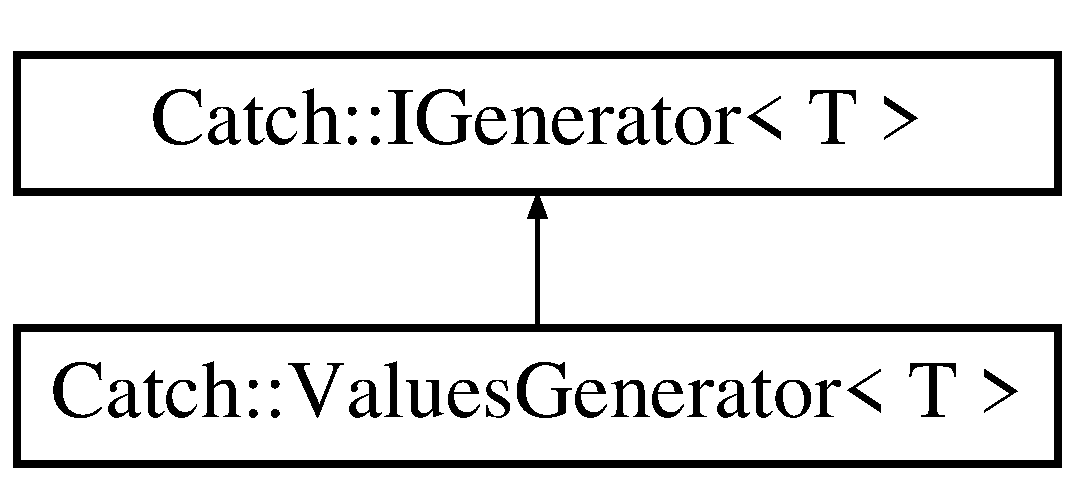
\includegraphics[height=2.000000cm]{class_catch_1_1_values_generator}
\end{center}
\end{figure}
\subsection*{Public Member Functions}
\begin{DoxyCompactItemize}
\item 
\hypertarget{class_catch_1_1_values_generator_a8412c8ce5d9d4fc6ff06d5246d56d538}{void {\bfseries add} (T value)}\label{class_catch_1_1_values_generator_a8412c8ce5d9d4fc6ff06d5246d56d538}

\item 
\hypertarget{class_catch_1_1_values_generator_a60599dd67096ff108471f64ee42acd9d}{virtual T {\bfseries get\-Value} (std\-::size\-\_\-t index) const }\label{class_catch_1_1_values_generator_a60599dd67096ff108471f64ee42acd9d}

\item 
\hypertarget{class_catch_1_1_values_generator_a98a80bb0dd682c44e82e4a75e98c4682}{virtual std\-::size\-\_\-t {\bfseries size} () const }\label{class_catch_1_1_values_generator_a98a80bb0dd682c44e82e4a75e98c4682}

\end{DoxyCompactItemize}


The documentation for this class was generated from the following file\-:\begin{DoxyCompactItemize}
\item 
Catch.\-h\end{DoxyCompactItemize}

\hypertarget{struct_catch_1_1_verbosity}{\section{Catch\-:\-:Verbosity Struct Reference}
\label{struct_catch_1_1_verbosity}\index{Catch\-::\-Verbosity@{Catch\-::\-Verbosity}}
}
\subsection*{Public Types}
\begin{DoxyCompactItemize}
\item 
enum {\bfseries Level} \{ {\bfseries No\-Output} = 0, 
{\bfseries Quiet}, 
{\bfseries Normal}
 \}
\end{DoxyCompactItemize}


The documentation for this struct was generated from the following file\-:\begin{DoxyCompactItemize}
\item 
Catch.\-h\end{DoxyCompactItemize}

\hypertarget{struct_catch_1_1_warn_about}{\section{Catch\-:\-:Warn\-About Struct Reference}
\label{struct_catch_1_1_warn_about}\index{Catch\-::\-Warn\-About@{Catch\-::\-Warn\-About}}
}
\subsection*{Public Types}
\begin{DoxyCompactItemize}
\item 
enum {\bfseries What} \{ {\bfseries Nothing} = 0x00, 
{\bfseries No\-Assertions} = 0x01
 \}
\end{DoxyCompactItemize}


The documentation for this struct was generated from the following file\-:\begin{DoxyCompactItemize}
\item 
Catch.\-h\end{DoxyCompactItemize}

%--- End generated contents ---

% Index
\newpage
\phantomsection
\addcontentsline{toc}{part}{Index}
\printindex

\end{document}
